\documentclass[12pt,leqno,twoside]{article}
\usepackage[textwidth=5.8in,hcentering,top=1in,bottom=1in]{geometry}
\linespread{1.2}
\raggedbottom
\usepackage{amsmath,amssymb,amsthm,mathtools,booktabs,array,graphicx,longtable}
\allowdisplaybreaks
\clubpenalty=10000
\widowpenalty=10000
\usepackage[T1]{fontenc}
\usepackage{lmodern,microtype}
\usepackage{placeins,needspace,afterpage}
\renewcommand{\topfraction}{0.9}
\renewcommand{\textfraction}{0.08}
\usepackage{xcolor}
\usepackage{pgfplots}
\pgfplotsset{compat=1.18}
\usetikzlibrary{calc}
\usepackage{newunicodechar}
\newunicodechar{∀}{\ensuremath{\forall}}
\newunicodechar{ᵐ}{\textsuperscript{m}}
\newunicodechar{ω}{\ensuremath{\omega}}
\newunicodechar{∂}{\ensuremath{\partial}}
\newunicodechar{ℝ}{\ensuremath{\mathbb R}}
\usepackage[nottoc,notlot,notlof]{tocbibind}
\usepackage{hyperref}
\hypersetup{colorlinks=true, allcolors=[rgb]{0.0,0.2,0.6}, linktoc=all}
\makeatletter\g@addto@macro\UrlBreaks{\do\_}\makeatother
\usepackage{fancyhdr}
\fancyhf{}
\fancyhead[CE]{\footnotesize\scshape s.\ kawada}
\fancyhead[CO]{\footnotesize\scshape radial laws for nested random polynomials}
\fancyhead[LE,RO]{\footnotesize\thepage}
\renewcommand{\headrulewidth}{0pt}
\renewcommand{\footrulewidth}{0pt}
\pagestyle{fancy}
\newcommand{\Prob}{\mathbb P}
\newcommand{\E}{\mathbb E}
\newcommand{\dd}{\,\mathrm d}
\newcommand{\C}{\mathbb C}
\makeatletter
\newcommand{\itemlabel}[2]{\item[(#1)]\protected@edef\@currentlabel{\thetheorem(#1)}\label{#2}}
\makeatother
\newtheorem{theorem}{Theorem}[section]
\newtheorem{lemma}[theorem]{Lemma}
\newtheorem{proposition}[theorem]{Proposition}
\newtheorem{corollary}[theorem]{Corollary}
\newtheorem{problem}[theorem]{Problem}
\newtheoremstyle{named}{\topsep}{\topsep}{\normalfont}{}{\bfseries}{.}{ }{\thmnote{#3}}
\theoremstyle{named}
\newtheorem*{namedhypothesis}{}
\theoremstyle{remark}
\newtheorem{remark}[theorem]{Remark}
\title{\Large Almost-Sure Radial Laws for Nested Random Polynomials\\
 and Erd\H{o}s Problem \#522}
\author{Sebastien Kawada\\[2pt]
 {\normalsize MIT CSAIL}\\[2pt]
 {\normalsize\texttt{kawada@csail.mit.edu}}}
\date{September 22, 2026}
\pdfsuppressptexinfo=-1
\hypersetup{
 pdftitle={Almost-Sure Radial Laws for Nested Random Polynomials and Erd\H{o}s Problem \#522},
 pdfauthor={Sebastien Kawada},
 pdfsubject={2020 Mathematics Subject Classification: Primary 60F15, 30C15; Secondary 30B20, 26C10, 60G50, 68V20},
 pdfkeywords={Random polynomials, Littlewood polynomials, random power series, zeros, almost sure convergence, Erd\H{o}s problems, Jensen's formula, Rouch\'e's theorem, formal verification, Lean}
}
\begin{document}
\maketitle
\begin{abstract}
Let $(a_k)_{k\ge0}$ be independent Rademacher random variables and let
$f_n(z)=\sum_{k=0}^n a_k z^k$. Erd\H{o}s asked in 1961 whether, almost surely, these
random Littlewood polynomials have $n/2+o(n)$ zeros in the closed unit disk, counted
with multiplicity, as $n\to\infty$. Here, we answer this question, Erd\H{o}s Problem
\#522, in the affirmative. In fact, we prove that, almost surely,
$\frac1n\#\{z:f_n(z)=0,\ |z|\le 1+x/n\}$ converges, at the natural scale $1/n$ around
the unit circle, uniformly on compact subsets of $\mathbb{R}$ to
$\frac12(1+\coth x-1/x)$, interpreted as $1/2$ when $x=0$. The same unit-disk and
radial laws hold when the coefficients are independent and identically distributed
with the Steinhaus distribution, the standard real Gaussian, the standard complex
Gaussian, or any nondegenerate distribution which is bounded and centrally symmetric.
For Rademacher coefficients we also prove the stronger almost sure bound
$\#\{z:f_n(z)=0,\ |z|\le 1\}=n/2+O(n/\log n)$. Since different degrees share their
coefficients, we first prove the result along a subsequence of degrees, and then fill
in the other degrees with Rouch\'e's theorem, once we show that few zeros near the
unit circle have a small derivative. All main results have been formally verified in
Lean.
\end{abstract}
\begin{quotation}\footnotesize\noindent
\emph{2020 Mathematics Subject Classification.} Primary 60F15, 30C15;
Secondary 30B20, 26C10, 60G50, 68V20.\par\nobreak\smallskip
\noindent\emph{Key words and phrases.} Random polynomials, Littlewood
polynomials, random power series, zeros, almost sure convergence,
Erd\H{o}s problems, Jensen's formula, Rouch\'e's theorem, formal
verification, Lean.
\end{quotation}

\Needspace{10\baselineskip}
\tableofcontents

\section{Introduction}\label{sec:introduction}
We consider random polynomials whose coefficients are taken from the
same sequence for every degree. Throughout, zeros are counted with
multiplicity. Our main result is the following radial law.

\begin{theorem}[Radial law]\label{thm:radial-profile}
Let $(\xi_k)_{k\ge0}$ be independent and identically distributed, with
the Rademacher, Steinhaus, standard real Gaussian or standard complex
Gaussian distribution, or with a nondegenerate bounded centrally
symmetric distribution on $\mathbb R$ or $\mathbb C$. Put
$f_n(z)=\sum_{k=0}^n\xi_kz^k$, let $\nu_n(r)$ be the number of zeros of
$f_n$ in $\{|z|\le r\}$, counted with multiplicity, with $\nu_n=0$ when
$f_n\equiv0$, and put
\[
 \Phi(x)=\frac{\int_0^1t e^{2xt}\dd t}
                   {\int_0^1e^{2xt}\dd t}.
\]
On one event of probability one, for every $A>0$,
\[
 \lim_{n\to\infty}\sup_{|x|\le A}
 \left|\frac{\nu_n(1+x/n)}n-\Phi(x)\right|=0.
\]
Explicitly,
\[
 \Phi(0)=\tfrac12,\qquad
 \Phi(x)=\frac{e^{2x}}{e^{2x}-1}-\frac1{2x}\quad(x\ne0).
\]
\end{theorem}
\afterpage{\begin{figure}[t]
\centering
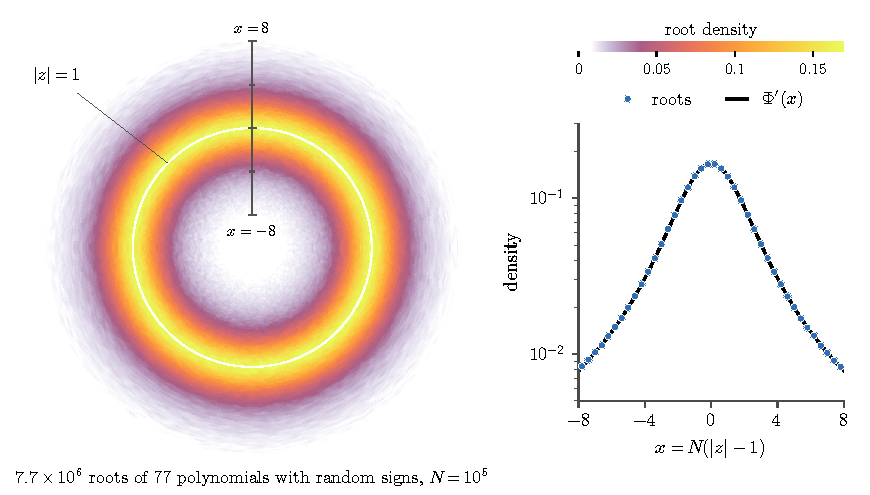
\includegraphics[width=\textwidth]{figures/explanatory/radial-density.pdf}
\caption{Density of the zeros of 77 random Littlewood polynomials of degree
$10^5$ near the unit circle (left), and its angular average with the
limiting density $\Phi'$ (right).}
\label{fig:radial-density}
\end{figure}
}

We prove Theorem~\ref{thm:radial-profile} for Rademacher coefficients in
Section~\ref{sec:layer3}, and for the other distributions in
Section~\ref{sec:layer2-models}.
Here the Rademacher distribution gives $\pm1$ with probability $\frac12$
each, the Steinhaus distribution is uniform on the unit circle, and the
standard complex Gaussian distribution has density $\pi^{-1}e^{-|z|^2}$
on $\C$.

In particular, almost surely we have $\nu_n(1+x/n)/n\to\Phi(x)$
simultaneously for every $x\in\mathbb R$, and the convergence is uniform
on each compact interval of $x$.
To obtain the explicit formula, note that the quotient defining $\Phi$
is the derivative of $\frac12\log\int_0^1e^{2xt}\dd t$, and that
$\int_0^1e^{2xt}\dd t=(e^{2x}-1)/(2x)$ for $x\ne0$, so that
\[
 \Phi(x)=\frac{\mathrm d}{\mathrm dx}\,\frac12\log\frac{e^{2x}-1}{2x}
 =\frac{e^{2x}}{e^{2x}-1}-\frac1{2x}
 =\frac12\Big(1+\coth x-\frac1x\Big).
\]
In particular $\Phi(x)\to0$ as $x\to-\infty$ and $\Phi(x)\to1$ as
$x\to\infty$.
In Figure~\ref{fig:radial-density} we compare the limiting density
$\Phi'$ with the roots of 77 polynomials with random signs.
Taking $x=0$ in Theorem~\ref{thm:radial-profile}, we obtain the following
strong law.

\begin{corollary}[The unweighted strong law]\label{thm:stronglaw}
In the setting of Theorem~\ref{thm:radial-profile}, almost surely
\[
 \frac{\nu_n(1)}n\longrightarrow\frac12.
\]
\end{corollary}

For Rademacher coefficients, in the notation of Erd\H{o}s problem
\#522~\cite{Erdos522Problem}, where $R_n=\nu_n(1)$ is the number of roots
in the closed unit disk, Corollary~\ref{thm:stronglaw} states that
$R_n/(n/2)\to1$ almost surely.
For these coefficients we first prove Corollary~\ref{thm:stronglaw} directly in
Section~\ref{sec:unit-circle}, and then we prove
Theorem~\ref{thm:radial-profile} in Section~\ref{sec:moving-radii} by the
same construction.

For Rademacher coefficients we also obtain a rate of convergence in the
unit disk.

\begin{theorem}[Logarithmic rate]\label{thm:log-rate}
In the setting of Theorem~\ref{thm:radial-profile}, for Rademacher
coefficients,
\[
 \limsup_{n\to\infty}(\log n)
       \left|\frac{\nu_n(1)}n-\frac12\right|
       \le 2000\log2\qquad\hbox{almost surely}.
\]
\end{theorem}

In Section~\ref{sec:extensions} we also determine sufficient exponents
for a sparse subsequence of degrees in the construction
(Proposition~\ref{prop:sparse-exponents}), bound the number of roots in
sublevel components that meet circles near the unit circle
(Corollary~\ref{cor:crossings}), and compute the logarithmic variance
profile of polynomially weighted polynomials with random signs
(Proposition~\ref{prop:weighted-log-variance-profile}).

The question of convergence in probability appears in Hayman's problem
collection~\cite[Problem 4.15]{Hayman1967,HaymanLingham2018}.
Yakir~\cite{Yakir2022} proved that the proportion of roots in the unit
disk converges to $1/2$ in probability, by combining concentration of an
angular logarithmic integral with Jensen's formula.
In his convention of $n$ coefficients, with probability tending to one,
the number of roots in the unit disk differs from $n/2$ by less than
$n^{9/10}$.
Do~\cite{Do2024} proved that, for nested Kac polynomials with iid real
coefficients of mean zero, variance one, and finite
$(2+\varepsilon)$th moment, the number of real roots in $[-1,1]$, divided by $\log n$, tends
to $1/\pi$ almost surely.
That proof uses maximal inequalities to pass from a sparse subsequence of
degrees to all degrees.
For the complex roots considered here, we compare
consecutive degrees by root matching under the appended coefficient tail.

\paragraph{Conventions.}
Sections~\ref{sec:radial}--\ref{sec:layer3} treat Rademacher
coefficients, which we write $\epsilon_k$, and
Section~\ref{sec:layer2-models} treats the other distributions, whose
coefficients we write $\xi_k$.
In $\nu_n(r)$ the disk is closed, and the denominator in every limit is
the nominal degree $n$.
For a coefficient distribution with an atom at zero,
$\nu_n=0$ whenever $f_n$ is identically zero.
The radii $1+x/n$ with $|x|\le A$ are positive once $n>A$, and only
sufficiently large $n$ are used when $x<0$.
We write $C(K)$ for a positive constant depending only on the parameter
$K$, which may increase from one estimate to the next, and $\log$ for the
natural logarithm.
Whenever $j$ indexes blocks of degrees, $N=j^8$ is the first degree of the
block $j^8\le n<(j+1)^8$, except in the proof of
Proposition~\ref{prop:sparse-exponents}, where $N=\lfloor j^q\rfloor$.
We call these first degrees the sparse subsequence of degrees.
We write $\mu$ for the normalized arc measure $\mathrm d\theta/(2\pi)$ on the
circle $\mathbb T$ of angles $\theta$.


\subsection*{The proof}
The main difficulty is to pass from the sparse subsequence of degrees to
every degree, which requires control of root movement under every partial
appended tail.
We first show that most roots lie in a narrow annulus, and then control
the roots at which the derivative is small.
Figure~\ref{fig:proof-map} shows how these steps depend on one another.

We first estimate the angular average of the logarithm of the normalized
polynomial (Theorem~\ref{thm:sign-logarithms}).
For this we use one-point and two-point Gaussian approximations to the
occupation of small disks by that polynomial.
Logarithmic integrability controls the contribution near zero.
Along the sparse subsequence of degrees, the resulting probability bounds
are summable.
By Jensen's formula at four radii (Lemmas~\ref{thm:T2}
and~\ref{lem:annular-mass}, and Corollary~\ref{cor:radial-probability}) we
get
\[
 \frac1N\#\{\alpha:f_N(\alpha)=0,\ ||\alpha|-1|>K/N\}
 \le\frac{2\log2}{K}+o(1),
\]
so that $K$ controls the fraction of roots outside the annulus.

For each root in this annulus with small derivative there is a nearby
mesh point at which the polynomial and its derivative are both small.
We bound the first two moments of the number of these mesh points
through the covariance matrices of the corresponding real random
vectors, which have four coordinates for one mesh point and eight for a
pair.
To bound the number of roots assigned to one mesh point, we use
Hanson--Wright concentration for arc energy and Jensen's formula.
By Lemma~\ref{lem:small-derivatives}, outside a summable exceptional
event there are at most $N^{31/32}$ annular roots with
$|f_N'(\alpha)|<N^{3/2-1/64}$.

We localize each remaining root by a Taylor expansion
(Lemma~\ref{lem:isolation-interface}).
A common regular sublevel of $|f_N|$ then yields disjoint domains, each
of which contains one root.
We compare every degree $n$ of a block $j^8\le n<(j+1)^8$ with its
first degree $N=j^8$.
By a maximal bound on every appended tail (Lemma~\ref{lem:tails}), the
hypothesis of Rouch\'e's theorem holds on the boundary of each selected
domain.
The tail amplitude controls the localization radius.
The exponent eight ensures that the probability bounds are summable and
that the localization radius is smaller than the half-width of the thin
band.

By root matching (Theorem~\ref{thm:T4}) we have
\[
 |\nu_n(1)-\nu_N(1)|\le c_N+U_N+(\deg f_n-\deg f_N),
\]
where $c_N$ is the number of selected domains whose closures meet the
unit circle and $U_N$ is the number of unselected roots.
Through the thin bands of Lemma~\ref{lem:thin-band}, the same
logarithmic concentration estimate shows that the normalized count of the
roots in the crossing domains tends to zero, since these roots lie in a
thinner annulus.
The unselected roots contribute at most $2\log2/K+o_K(1)$ to the
normalized count.
For each fixed $K$ the probabilities of the exceptional events are
summable over the blocks, so that by the Borel--Cantelli lemma these
bounds hold for all large blocks on an event $\Omega_K$ of probability
one.
Finally, we let $K$ tend to infinity on $\bigcap_{K\ge2}\Omega_K$, which
yields the limit along all degrees on the original probability space.

In the probabilistic estimates we use Rai\v{c}'s convex-set normal
approximation~\cite{Raic2019}, the logarithmic integrability of
Nazarov--Nishry--Sodin~\cite{NNS2013}, and the Hanson--Wright
inequality~\cite{RudelsonVershynin2013}.
We compute the constants and their dependence on the annular width in
Appendix~\ref{sec:constants}.

The Lean formalization~\cite{FormalCompanion2026} proves the unit-disk
and radial laws on the shared coefficient space.
Appendix~\ref{sec:formalization} describes the theorem correspondence.
\afterpage{\begin{figure}[t]
\centering
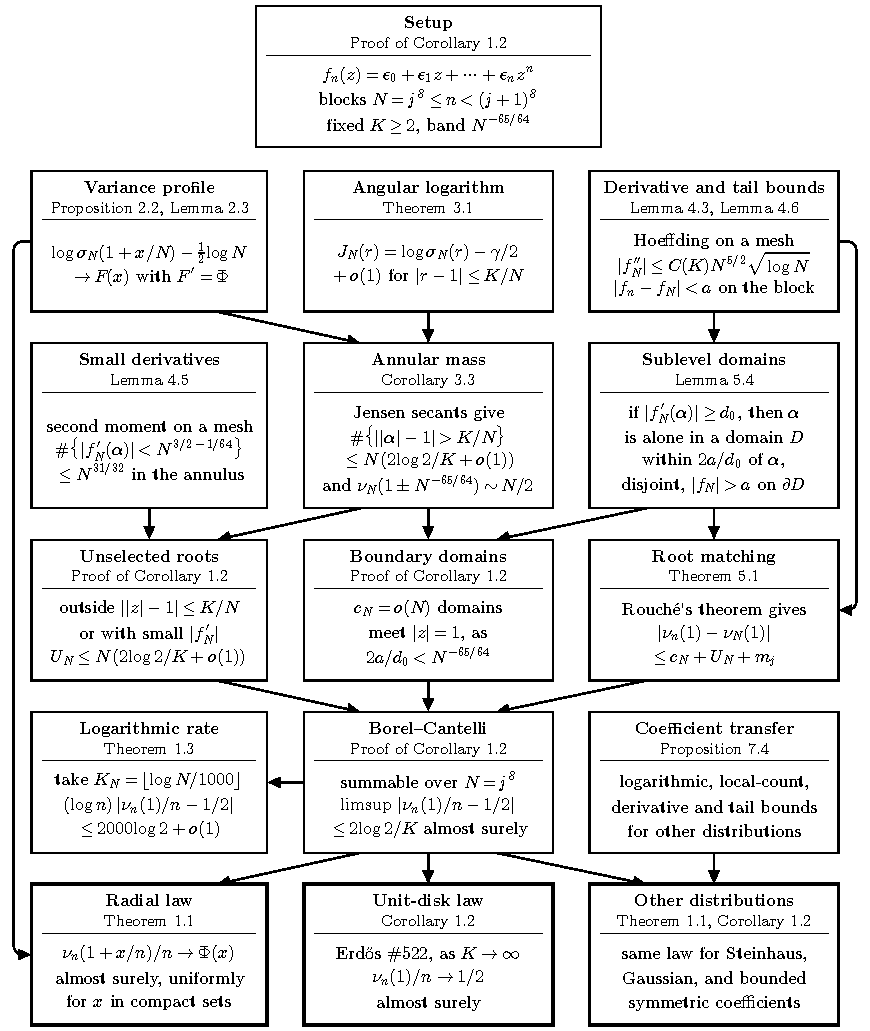
\includegraphics[width=0.97\textwidth]{figures/explanatory/proof-map.pdf}
\caption{Structure of the proof. Arrows point from inputs to the steps that
use them.}
\label{fig:proof-map}
\end{figure}
}

\subsection*{Organization}
In Section~\ref{sec:radial} we apply Jensen's formula to radial counts and
compute the variance profile, and in Section~\ref{sec:concentration} we
prove logarithmic concentration for signs.
Section~\ref{sec:local-roots} contains the local-count, derivative, and
maximal-tail estimates.
We prove root matching in Section~\ref{sec:matching}, and then
Corollary~\ref{thm:stronglaw} and Theorem~\ref{thm:radial-profile} in
Section~\ref{sec:layer3}.
In Section~\ref{sec:layer2-models} we treat the other coefficient
distributions and prove Theorem~\ref{thm:radial-profile} and
Corollary~\ref{thm:stronglaw} for them.
The rate, the choice of the sparse subsequence of degrees, nearby circles,
and weighted variance profiles follow in Section~\ref{sec:extensions}.
Section~\ref{sec:open-problems} collects open problems, and
Section~\ref{sec:numerics} reports numerical observations.
In Appendix~\ref{sec:general-estimates} we collect the general forms of
the concentration, mesh, and diagonalization estimates.


\section{Jensen's formula and the variance profile}\label{sec:radial}

By Jensen's formula, the number of roots in a disk is the slope of the
angular logarithm $J_N(e^t)$, a convex function of $t$, so bounds on
$J_N$ at four radii bound the roots outside an annulus. Replacing $J_N$
by its Gaussian value, which Proposition~\ref{prop:profiles} computes,
gives the limiting fraction. Let $f_N(z)=\sum_{k=0}^N\epsilon_kz^k$, and
set
\[
 \sigma_N(r)^2=\sum_{k=0}^Nr^{2k},\qquad
 J_N(r)=\int_{\mathbb T}\log|f_N(re^{i\theta})|\dd\mu(\theta).
\]
The results of this section hold for every nonzero polynomial $f_N$ of
degree at most $N$; randomness enters only through
Section~\ref{sec:concentration}. We write $\gamma$ for Euler's constant.

\begin{lemma}[Four-radius bound for radial mass]\label{thm:T2}
Let $f_N$ be a nonzero polynomial of degree at most $N$, and fix $K>0$,
$0<\eta<1$ and $N>K$. We set
\[
 (x_1,x_2,x_3,x_4)=(-K,-(1-\eta)K,(1-\eta)K,K),\qquad r_i=1+x_i/N.
\]
Let $\sigma_N(r)>0$ be a normalization, and suppose that at each of these
four radii
\begin{equation}
 \left|J_N(r_i)-\log\sigma_N(r_i)+\gamma/2\right|\leq\varepsilon_i,
 \qquad i=1,2,3,4. \label{eq:four-radius-log-errors}
\end{equation}
Then
\begin{align}
 \frac{\#\{\alpha:f_N(\alpha)=0,\ ||\alpha|-1|>K/N\}}N
 &\leq\frac{\deg f_N}N\nonumber\\
 &\quad+\frac{\log\sigma_N(r_2)-\log\sigma_N(r_1)+\varepsilon_1+\varepsilon_2}{N\log(r_2/r_1)}\nonumber\\
 &\quad-\frac{\log\sigma_N(r_4)-\log\sigma_N(r_3)-\varepsilon_3-\varepsilon_4}{N\log(r_4/r_3)}.\label{eq:T2-exact}
\end{align}
In particular, suppose that along a sequence of degrees $\deg f_N/N\to1$, that
the errors $\varepsilon_i$ tend to zero, and that $\log\sigma_N(1+x/N)$,
minus a deterministic centering that may depend on $N$ but not on $x$,
converges to $F(x)$ uniformly on $[-K,K]$.
Then the limiting upper bound for
$\#\{\alpha:f_N(\alpha)=0,\ ||\alpha|-1|>K/N\}/N$ is
\begin{equation}
 1+\frac1{\eta K}\{F(-(1-\eta)K)-F(-K)-F(K)+F((1-\eta)K)\}. \label{eq:T2-limit}
\end{equation}
\end{lemma}

We call $r_1,\dots,r_4$ the secant radii. Here the centering $-\gamma/2$ is $\E\log|G|$, where $G$ has density
$\pi^{-1}e^{-|z|^2}$ on $\C$, and it is the same at all four radii.
If the four bounds \eqref{eq:four-radius-log-errors} hold outside four
exceptional events, then \eqref{eq:T2-exact} holds outside their union,
whose probability is at most the sum of their probabilities.
The limiting bound \eqref{eq:T2-limit} holds for every sample sequence on
which the four bounds hold for all sufficiently large degrees.

\begin{proof}
We bound the roots in $\{|z|<r_1\}$ and in $\{|z|>r_4\}$ by the slopes
of two secants of the convex function $t\mapsto J_N(e^t)$, and then
replace $J_N$ by $\log\sigma_N$ using \eqref{eq:four-radius-log-errors}.
Write $f_N(z)=a\prod_{j=1}^{\deg f_N}(z-\alpha_j)$.
By Jensen's formula \cite[\S3.61]{Titchmarsh1939} for one factor,
$\int_{\mathbb T}\log|e^te^{i\theta}-\alpha|\dd\mu(\theta)=\max(t,\log|\alpha|)$
for $\alpha\ne0$, and the integral is $t$ for $\alpha=0$, so that
\[
 J_N(e^t)=\log|a|+\sum_{j=1}^{\deg f_N}\max(t,\log|\alpha_j|),
 \qquad t\in\mathbb R,
\]
where a term with $\alpha_j=0$ is read as $t$. The term of $\alpha_j$ has
right derivative $1$ if $|\alpha_j|\le e^t$ and $0$ otherwise, so
$t\mapsto J_N(e^t)$ is convex and piecewise linear with right derivative
$\nu_N(e^t)$. Integrating it and substituting $r=e^s$, we get
\begin{equation}
 J_N(e^{t'})-J_N(e^t)=\int_t^{t'}\nu_N(e^s)\dd s
 =\int_{e^t}^{e^{t'}}\frac{\nu_N(r)}r\dd r,\qquad t<t'.
 \label{eq:jensen-integral}
\end{equation}

Since $N>K$, we have $0<r_1<r_2<r_3<r_4$, and since $\nu_N$ is
nondecreasing, \eqref{eq:jensen-integral} gives
\begin{align*}
 \nu_N(r_1)
 &\leq\frac1{\log(r_2/r_1)}\int_{r_1}^{r_2}\frac{\nu_N(r)}r\dd r
 =\frac{J_N(r_2)-J_N(r_1)}{\log(r_2/r_1)},\\
 \frac{J_N(r_4)-J_N(r_3)}{\log(r_4/r_3)}
 &=\frac1{\log(r_4/r_3)}\int_{r_3}^{r_4}\frac{\nu_N(r)}r\dd r
 \leq\nu_N(r_4).
\end{align*}
By \eqref{eq:four-radius-log-errors}, in which $\gamma/2$ cancels in
differences, we have
\begin{align*}
 J_N(r_2)-J_N(r_1)
 &\leq\log\sigma_N(r_2)-\log\sigma_N(r_1)+\varepsilon_1+\varepsilon_2,\\
 J_N(r_4)-J_N(r_3)
 &\geq\log\sigma_N(r_4)-\log\sigma_N(r_3)-\varepsilon_3-\varepsilon_4.
\end{align*}

Let $m$ be the number of roots with $||\alpha|-1|>K/N$. At most
$\nu_N(r_1)$ of them lie in $\{|z|<r_1\}$ and exactly
$\deg f_N-\nu_N(r_4)$ in $\{|z|>r_4\}$, so by the last two displays
\begin{align*}
 \frac mN
 &\leq\frac{\nu_N(r_1)}N+\frac{\deg f_N-\nu_N(r_4)}N
 \leq\frac{\deg f_N}N
   +\frac{J_N(r_2)-J_N(r_1)}{N\log(r_2/r_1)}
   -\frac{J_N(r_4)-J_N(r_3)}{N\log(r_4/r_3)}\\
 &\leq\frac{\deg f_N}N
   +\frac{\log\sigma_N(r_2)-\log\sigma_N(r_1)+\varepsilon_1+\varepsilon_2}{N\log(r_2/r_1)}\\
 &\quad-\frac{\log\sigma_N(r_4)-\log\sigma_N(r_3)-\varepsilon_3-\varepsilon_4}{N\log(r_4/r_3)}.
\end{align*}
This proves \eqref{eq:T2-exact}.

For the limit, let $c$ be the centering of the hypothesis and
$F_N(x)=\log\sigma_N(1+x/N)-c$, so that $\log\sigma_N(r_i)=F_N(x_i)+c$.
Then
\begin{align*}
 N\log(r_2/r_1)&=\int_{-K}^{-(1-\eta)K}\frac{\mathrm dx}{1+x/N}\longrightarrow\eta K,\\
 N\log(r_4/r_3)&=\int_{(1-\eta)K}^{K}\frac{\mathrm dx}{1+x/N}\longrightarrow\eta K.
\end{align*}
Since $c$ cancels in differences, the right-hand side of
\eqref{eq:T2-exact} is the first line below, and since $\deg f_N/N\to1$,
$\varepsilon_i\to0$ and $F_N(x_i)\to F(x_i)$,
\begin{align*}
 &\frac{\deg f_N}N
   +\frac{F_N(x_2)-F_N(x_1)+\varepsilon_1+\varepsilon_2}{N\log(r_2/r_1)}
 -\frac{F_N(x_4)-F_N(x_3)-\varepsilon_3-\varepsilon_4}{N\log(r_4/r_3)}\\
 &\qquad\longrightarrow1+\frac{F(x_2)-F(x_1)}{\eta K}-\frac{F(x_4)-F(x_3)}{\eta K},
\end{align*}
so that the limit superior of $m/N$ is at most \eqref{eq:T2-limit}.
\end{proof}

Figure~\ref{fig:jensen-secants} shows these secants for one sequence at $N=10^5$.
Section~\ref{sec:log-rate} lets $\eta$ tend to zero with $N$, and all
other uses take $\eta=1/2$.

\begin{figure}[t]
\centering
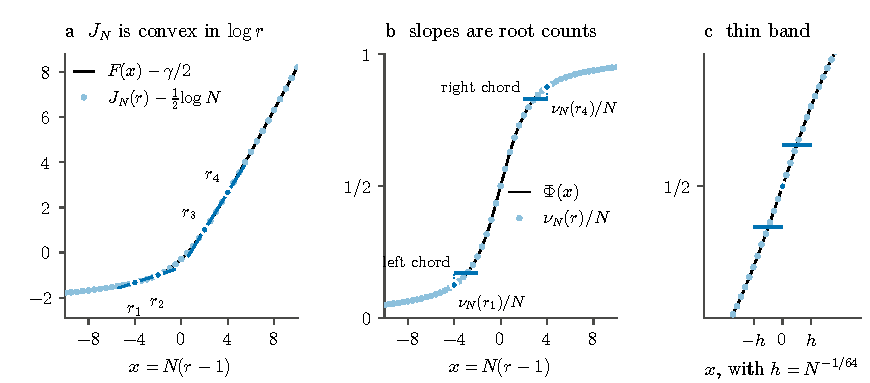
\includegraphics[width=\textwidth]{figures/explanatory/jensen-secants.pdf}
\caption{Jensen secants for one sequence at $N=10^5$. The chord slopes bound
the normalized zero counts, which approach $\Phi$.}
\label{fig:jensen-secants}
\end{figure}


\begin{proposition}[The unweighted logarithmic variance profile]\label{prop:profiles}
For the normalization $\sigma_N(r)^2=\sum_{k=0}^Nr^{2k}$ of this section,
\[
 \log\sigma_N(1+x/N)-\tfrac12\log N\longrightarrow
 F(x):=\frac12\log\int_0^1e^{2xt}\dd t
\]
uniformly on compact intervals of $x$. The profile satisfies
\[
 F'(x)=\Phi(x),\qquad F(x)=x+F(-x),\qquad F'(0)=\tfrac12.
\]
For $0<\eta<1$, the bound in \eqref{eq:T2-limit} is
\begin{equation}
 \frac2{\eta K}\{F(-(1-\eta)K)-F(-K)\}
 =\frac1{\eta K}\log\frac{1-e^{-2(1-\eta)K}}{(1-\eta)(1-e^{-2K})}
 \le\frac1{\eta K}\log\frac1{1-\eta},
 \label{eq:profile-eta-bound}
\end{equation}
which at $\eta=1/2$ is
\[
 \frac2K\log\frac{2}{1+e^{-K}}\leq\frac{2\log2}{K}.
\]
\end{proposition}

\begin{proof}
We first compare each term $(1+x/N)^{2k}$ of $\sigma_N(1+x/N)^2$ with
$e^{2xk/N}$, which turns $\sigma_N(1+x/N)^2/N$ into a Riemann sum for
$\int_0^1e^{2xt}\dd t$, and then derive the identities for $F$ and the
value of \eqref{eq:T2-limit} from this integral.

For $|x|\leq K$, $N\geq2K$ and $0\leq k\leq N$, expanding the logarithm
in its power series and using $|x/N|\le K/N\le1/2$, we obtain
\begin{align*}
 &\left|2k\log(1+x/N)-2xk/N\right|
 =2k\left|-\frac12\Big(\frac xN\Big)^2+\frac13\Big(\frac xN\Big)^3-\cdots\right|\\
 &\qquad\le k\Big(\frac xN\Big)^2\Big(1+\Big|\frac xN\Big|+\Big(\frac xN\Big)^2+\cdots\Big)
 =\frac{k(x/N)^2}{1-|x/N|}\le2k\Big(\frac xN\Big)^2\le2K^2/N.
\end{align*}
Exponentiating, we get
\begin{equation}
 e^{-2K^2/N}\leq
 \frac{(1+x/N)^{2k}}{e^{2xk/N}}\leq e^{2K^2/N}.
 \label{eq:profile-comparison}
\end{equation}

Since $(x,t)\mapsto e^{2xt}$ is uniformly continuous on
$[-K,K]\times[0,1]$ and the term $k=0$ is $1/N$, the Riemann sums
$\frac1N\sum_{k=0}^Ne^{2xk/N}$ converge to $\int_0^1e^{2xt}\dd t$
uniformly for $|x|\leq K$. Multiplying \eqref{eq:profile-comparison} by
$e^{2xk/N}/N$ and summing over $0\le k\le N$, we see that
$\sigma_N(1+x/N)^2/N=\frac1N\sum_{k=0}^N(1+x/N)^{2k}$ lies between
$e^{-2K^2/N}$ and $e^{2K^2/N}$ times the Riemann sum, so that it has the
same limit. Since this limit is at least $e^{-2K}$ and the logarithm is
uniformly continuous on $[e^{-2K}/2,\infty)$, we obtain, uniformly for
$|x|\le K$,
\[
 \log\sigma_N(1+x/N)-\tfrac12\log N
 =\frac12\log\frac{\sigma_N(1+x/N)^2}N
 \longrightarrow\frac12\log\int_0^1e^{2xt}\dd t
 =F(x).
\]

Differentiating the positive integral under the integral sign, we have
\[
 F'(x)=\frac12\,\frac{\int_0^12te^{2xt}\dd t}{\int_0^1e^{2xt}\dd t}
 =\frac{\int_0^1t e^{2xt}\dd t}{\int_0^1e^{2xt}\dd t}
 =\Phi(x),
\]
and in particular $F'(0)=\int_0^1t\dd t=\frac12$.
Thus $\Phi(x)$ is the mean of $t$ under the probability density
proportional to $e^{2xt}$ on $[0,1]$, so that $0\le\Phi\le1$, and
differentiating this mean under the integral sign we get
\begin{align}
 \Phi'(x)
 &=\frac{\mathrm d}{\mathrm dx}\,\frac{\int_0^1te^{2xt}\dd t}{\int_0^1e^{2xt}\dd t}
 =\frac{\int_0^12t^2e^{2xt}\dd t}{\int_0^1e^{2xt}\dd t}
  -\frac{\int_0^1te^{2xt}\dd t\int_0^12te^{2xt}\dd t}{\bigl(\int_0^1e^{2xt}\dd t\bigr)^2}\nonumber\\
 &=2\bigg(\frac{\int_0^1t^2e^{2xt}\dd t}{\int_0^1e^{2xt}\dd t}
  -\Big(\frac{\int_0^1te^{2xt}\dd t}{\int_0^1e^{2xt}\dd t}\Big)^2\bigg)
 =2\operatorname{Var}_x(t)\ge0,\label{eq:Phi-variance}
\end{align}
where $\operatorname{Var}_x(t)$ is the variance of $t$ under the same
density.
The change of variables $t\mapsto1-t$ gives the symmetry
\[
 F(x)=\frac12\log\int_0^1e^{2x(1-t)}\dd t
 =\frac12\log\Big(e^{2x}\int_0^1e^{-2xt}\dd t\Big)
 =x+F(-x).
\]
By integration we also obtain, for $y>0$, $\int_0^1e^{-2yt}\dd t=(1-e^{-2y})/(2y)$, and hence
\begin{align*}
 F(-(1-\eta)K)-F(-K)
 &=\frac12\log\frac{(1-e^{-2(1-\eta)K})/(2(1-\eta)K)}{(1-e^{-2K})/(2K)}\\
 &=\frac12\log\frac{1-e^{-2(1-\eta)K}}{(1-\eta)(1-e^{-2K})}
 \le\frac12\log\frac1{1-\eta},
\end{align*}
since $1-e^{-2(1-\eta)K}\le1-e^{-2K}$. At $\eta=1/2$ the expression
before the inequality is
\[
 F(-K/2)-F(-K)=\frac12\log\frac{2(1-e^{-K})}{1-e^{-2K}}
 =\frac12\log\frac2{1+e^{-K}}.
\]
By $F(x)=x+F(-x)$ at $x=K$ and at $x=(1-\eta)K$,
\begin{align*}
 F(K)-F((1-\eta)K)&=K+F(-K)-(1-\eta)K-F(-(1-\eta)K)\\
 &=\eta K+F(-K)-F(-(1-\eta)K),
\end{align*}
and substituting this into \eqref{eq:T2-limit} we get
\begin{align*}
 &1+\frac1{\eta K}\{F(-(1-\eta)K)-F(-K)-F(K)+F((1-\eta)K)\}\\
 &\qquad=1+\frac1{\eta K}\{2F(-(1-\eta)K)-2F(-K)-\eta K\}\\
 &\qquad=\frac2{\eta K}\{F(-(1-\eta)K)-F(-K)\},
\end{align*}
which is \eqref{eq:profile-eta-bound} by the evaluation of
$F(-(1-\eta)K)-F(-K)$ above, and at $\eta=1/2$ is
\[
 \frac2K\log\frac2{1+e^{-K}}\le\frac{2\log2}K.
\]
\end{proof}

This proof also yields a rate of convergence in the profile limit.

\begin{lemma}[Rate in the variance profile]\label{lem:profile-rate}
For $K>0$, $N\ge2K$ and $|x|\le K$,
\[
 \left|\log\sigma_N(1+x/N)-\tfrac12\log N-F(x)\right|
 \le\frac{K^2+e^{4K}/2}{N}.
\]
\end{lemma}

\begin{proof}
We use \eqref{eq:profile-comparison} to compare
$\sigma_N(1+x/N)^2/N$ with a Riemann sum of $e^{2xt}$, and the
monotonicity of $t\mapsto e^{2xt}$ to compare the Riemann sum with the
integral.
Let
\[
 S_N(x)=\frac1N\sum_{k=0}^Ne^{2xk/N},\qquad
 I(x)=\int_0^1e^{2xt}\dd t,
\]
so that $F=\frac12\log I$.
Multiplying \eqref{eq:profile-comparison} by $e^{2xk/N}/N$ and summing
over $0\le k\le N$, we get
$e^{-2K^2/N}S_N(x)\le\sigma_N(1+x/N)^2/N\le e^{2K^2/N}S_N(x)$, and hence
\[
 \left|\log\frac{\sigma_N(1+x/N)^2}N-\log S_N(x)\right|\le\frac{2K^2}N.
\]
The function $g(t)=e^{2xt}$ is nondecreasing on $[0,1]$ for $x\ge0$ and
nonincreasing for $x\le0$, so that $I(x)$ lies between the Riemann sums
$\frac1N\sum_{k=0}^{N-1}g(k/N)$ and $\frac1N\sum_{k=1}^Ng(k/N)$, in the
order that gives
\begin{align*}
 I(x)&\le\frac1N\sum_{k=1}^Ng(k/N)\le S_N(x)
 =\frac1N\sum_{k=0}^{N-1}g(k/N)+\frac{g(1)}N\le I(x)+\frac{g(1)}N,
 \qquad x\ge0,\\
 I(x)&\le\frac1N\sum_{k=0}^{N-1}g(k/N)\le S_N(x)
 =\frac1N\sum_{k=1}^Ng(k/N)+\frac{g(0)}N\le I(x)+\frac{g(0)}N,
 \qquad x\le0.
\end{align*}
In either case, since $g(0)=1$ and $g(1)=e^{2x}\le e^{2K}$,
\[
 I(x)\le S_N(x)\le I(x)+\frac{\max(g(0),g(1))}N\le I(x)+\frac{e^{2K}}N.
\]
For $|x|\le K$ we also have $I(x)\ge e^{-2K}$, since $e^{2xt}\ge e^{-2K}$
for $0\le t\le1$.
By the mean value theorem, $|\log a-\log b|\le|a-b|/\min(a,b)$ for
$a,b>0$, and hence
\[
 0\le\log S_N(x)-\log I(x)\le\frac{e^{2K}/N}{e^{-2K}}=\frac{e^{4K}}N.
\]
Combining the two estimates, we obtain
\begin{align*}
 &\left|\log\sigma_N(1+x/N)-\tfrac12\log N-F(x)\right|
 =\tfrac12\left|\log\frac{\sigma_N(1+x/N)^2}N-\log I(x)\right|\\
 &\qquad\le\tfrac12\left|\log\frac{\sigma_N(1+x/N)^2}N-\log S_N(x)\right|
   +\tfrac12\bigl|\log S_N(x)-\log I(x)\bigr|\\
 &\qquad\le\tfrac12\left(\frac{2K^2}N+\frac{e^{4K}}N\right)
 =\frac{K^2+e^{4K}/2}{N}.
\end{align*}
\end{proof}

Figure~\ref{fig:tilted-mean} shows $\Phi(x)$ as the mean of $t$ under
the limit, in $t=k/N$, of the tilted coefficient mass
$Nr^{2k}/\sigma_N(r)^2$ at $r=1+x/N$.

\afterpage{\begin{figure}[t]
\centering
\definecolor{oiblue}{HTML}{0072B2}
\colorlet{tiltTwo}{oiblue}%
\colorlet{tiltOne}{oiblue!45}%
\pgfmathdeclarefunction{tiltdens}{2}{%
  \pgfmathparse{2*(#1)*exp(2*(#1)*(#2))/(exp(2*(#1))-1)}}%
\pgfmathdeclarefunction{PhiFn}{1}{%
  \pgfmathparse{1/(1-exp(-2*(#1))) - 1/(2*(#1))}}%
\def\PhiTwo{0.768657}\def\PhiOne{0.656518}%
\def\PhiMOne{0.343482}\def\PhiMTwo{0.231343}%
\begin{tikzpicture}[
    font=\footnotesize,
    tilt/.style={line width=1pt},
    guide/.style={densely dotted, line width=0.6pt},
    meanpt/.style={circle, fill, inner sep=1.3pt},
  ]
\begin{axis}[
    name=a, scale only axis, width=4.7cm, height=5cm,
    xmin=0, xmax=4.4, ymin=0, ymax=1,
    axis lines=left, clip=false,
    xtick={0,1,2,3,4}, ytick={0,0.5,1}, yticklabels={$0$,$\tfrac12$,$1$},
    xlabel={$p_x(t)$}, ylabel={$t = k/N$},
    ylabel style={yshift=-4pt},
    title={\textbf{a}},
    title style={at={(0,1)}, anchor=south west, xshift=-18pt, yshift=6pt},
    every tick label/.append style={font=\fontsize{9}{11}\selectfont},
  ]
  \addplot[tiltTwo, tilt, domain=0:1, samples=120, variable=\t]
    ({tiltdens(2,\t)}, {\t});
  \addplot[tiltTwo, tilt, dashed, domain=0:1, samples=120, variable=\t]
    ({tiltdens(-2,\t)}, {\t});
  \addplot[tiltOne, tilt, domain=0:1, samples=80, variable=\t]
    ({tiltdens(1,\t)}, {\t});
  \addplot[tiltOne, tilt, dashed, domain=0:1, samples=80, variable=\t]
    ({tiltdens(-1,\t)}, {\t});
  \addplot[black, tilt] coordinates {(1,0) (1,1)};
  \coordinate (a2)  at (axis cs:{tiltdens(2,\PhiTwo)},\PhiTwo);
  \coordinate (a1)  at (axis cs:{tiltdens(1,\PhiOne)},\PhiOne);
  \coordinate (a0)  at (axis cs:1,0.5);
  \coordinate (am1) at (axis cs:{tiltdens(-1,\PhiMOne)},\PhiMOne);
  \coordinate (am2) at (axis cs:{tiltdens(-2,\PhiMTwo)},\PhiMTwo);
\end{axis}
\begin{axis}[
    name=b, at={($(a.south east)+(0.95cm,0)$)}, anchor=south west,
    scale only axis, width=7.5cm, height=5cm,
    xmin=-4.2, xmax=4.2, ymin=0, ymax=1,
    axis lines=left, clip=false,
    xtick={-4,-2,0,2,4}, ytick={0,0.5,1}, yticklabels={},
    xlabel={$x$},
    title={\textbf{b}},
    title style={at={(0,1)}, anchor=south west, yshift=6pt},
    every tick label/.append style={font=\fontsize{9}{11}\selectfont},
    legend style={draw=none, fill=none, font=\fontsize{9}{11}\selectfont, row sep=-1pt,
                  at={(1,0.02)}, anchor=south east},
    legend cell align=left,
  ]
  \addplot[forget plot, black, line width=1.3pt, domain=-4.2:-0.2, samples=90] {PhiFn(x)};
  \addplot[forget plot, black, line width=1.3pt, domain=-0.2:0.2, samples=9]
    {0.5 + x/6 - x^3/90};
  \addplot[forget plot, black, line width=1.3pt, domain=0.2:4.2, samples=90] {PhiFn(x)};
  \node[anchor=south east, font=\fontsize{9}{11}\selectfont] at (axis cs:4.2,{PhiFn(4.2)+0.02})
    {$\Phi(x)$};
  \coordinate (b2)  at (axis cs:2,\PhiTwo);
  \coordinate (b1)  at (axis cs:1,\PhiOne);
  \coordinate (b0)  at (axis cs:0,0.5);
  \coordinate (bm1) at (axis cs:-1,\PhiMOne);
  \coordinate (bm2) at (axis cs:-2,\PhiMTwo);
  \addlegendimage{tiltTwo, tilt}          \addlegendentry{$x=2$}
  \addlegendimage{tiltOne, tilt}          \addlegendentry{$x=1$}
  \addlegendimage{black, tilt}            \addlegendentry{$x=0$}
  \addlegendimage{tiltOne, tilt, dashed}  \addlegendentry{$x=-1$}
  \addlegendimage{tiltTwo, tilt, dashed}  \addlegendentry{$x=-2$}
\end{axis}
\foreach \s/\c in {2/tiltTwo, 1/tiltOne, 0/black, m1/tiltOne, m2/tiltTwo} {
  \draw[guide, \c] (a\s) -- (b\s);
  \node[meanpt, \c] at (a\s) {};
  \node[meanpt, \c] at (b\s) {};
}
\end{tikzpicture}
%
\caption{The densities $p_x(t)=2xe^{2xt}/(e^{2x}-1)$ (a) and their means
$\Phi(x)$ (b).}
\label{fig:tilted-mean}
\end{figure}
}

\subsection{Radial mass and thin bands}\label{sec:radial-mass}
In the next two lemmas we turn bounds on $J_N$ at a few radii into bounds
on root counts, and in Section~\ref{sec:concentration} these bounds are
supplied by Theorem~\ref{thm:sign-logarithms} outside exceptional events
with summable probabilities.

\begin{lemma}[Annular mass]\label{lem:annular-mass}
Let $K>0$, $0<\eta<1$ and $N\ge2K$, let $f_N$ be a nonzero polynomial of
degree at most $N$, and let $r_i=1+x_i/N$ with
$(x_1,x_2,x_3,x_4)=(-K,-(1-\eta)K,(1-\eta)K,K)$.
Let $\varepsilon,D\ge0$ be such that
\begin{align*}
 \left|J_N(r_i)-\log\sigma_N(r_i)+\gamma/2\right|&\le\varepsilon,\\
 \left|\log\sigma_N(r_i)-\tfrac12\log N-F(x_i)\right|&\le D/N,
 \qquad i=1,2,3,4.
\end{align*}
Then
\begin{align*}
 &\frac{\#\{\alpha:f_N(\alpha)=0,\ ||\alpha|-1|>K/N\}}N\\
 &\qquad\le\frac2{\eta K}\{F(-(1-\eta)K)-F(-K)\}
   +\frac4{\eta K}\Big(\varepsilon+\frac DN\Big)\\
 &\qquad\le\frac1{\eta K}\log\frac1{1-\eta}
   +\frac4{\eta K}\Big(\varepsilon+\frac DN\Big).
\end{align*}
In particular, for $\eta=1/2$,
\begin{align*}
 \frac{\#\{\alpha:f_N(\alpha)=0,\ ||\alpha|-1|>K/N\}}N
 &\le\frac2K\log\frac2{1+e^{-K}}+\frac8K\Big(\varepsilon+\frac DN\Big)\\
 &\le\frac{2\log2}K+\frac8K\Big(\varepsilon+\frac DN\Big).
\end{align*}
\end{lemma}

By Lemma~\ref{lem:profile-rate}, the second condition holds with
$D=K^2+e^{4K}/2$.

\begin{proof}
We divide the two secants of Lemma~\ref{thm:T2} by the linear spacing
$\eta K$ in place of the logarithmic one, replace $J_N$ by
$\frac12\log N+F$, and evaluate the leading term by
Proposition~\ref{prop:profiles}.
Let $m$ be the number of roots with $||\alpha|-1|>K/N$.
Since $0<1+x/N\le1$ for $-K\le x\le0$, because $N>K$, and
$1+x/N\ge1$ for $x\ge0$, the denominators satisfy
\begin{align*}
 N\log(r_2/r_1)&=\int_{-K}^{-(1-\eta)K}\frac{\mathrm dx}{1+x/N}\ge\eta K,\\
 N\log(r_4/r_3)&=\int_{(1-\eta)K}^{K}\frac{\mathrm dx}{1+x/N}\le\eta K.
\end{align*}
By \eqref{eq:jensen-integral}, $J_N(r)$ is nondecreasing in $r$, so that
the numerators $J_N(r_2)-J_N(r_1)$ and $J_N(r_4)-J_N(r_3)$ are
nonnegative. By the two hypotheses, in which $\gamma/2$ and
$\frac12\log N$ cancel in differences,
\begin{align*}
 J_N(r_2)-J_N(r_1)&\le F(x_2)-F(x_1)+2\Big(\varepsilon+\frac DN\Big),\\
 J_N(r_4)-J_N(r_3)&\ge F(x_4)-F(x_3)-2\Big(\varepsilon+\frac DN\Big).
\end{align*}
By the second inequality of the bound on $m/N$ in the proof of
Lemma~\ref{thm:T2}, $\deg f_N\le N$, the bounds on the denominators and
the two bounds above, we have
\begin{align*}
 \frac mN
 &\le1+\frac{J_N(r_2)-J_N(r_1)}{\eta K}-\frac{J_N(r_4)-J_N(r_3)}{\eta K}\\
 &\le1+\frac1{\eta K}\{F(x_2)-F(x_1)-F(x_4)+F(x_3)\}
 +\frac4{\eta K}\Big(\varepsilon+\frac DN\Big)\\
 &=\frac2{\eta K}\{F(-(1-\eta)K)-F(-K)\}
 +\frac4{\eta K}\Big(\varepsilon+\frac DN\Big),
\end{align*}
where the last line is the evaluation of \eqref{eq:T2-limit} in the proof
of Proposition~\ref{prop:profiles}, and \eqref{eq:profile-eta-bound}
bounds its first term.
\end{proof}

The two secants contribute equally to the leading term
$\frac2{\eta K}\{F(-(1-\eta)K)-F(-K)\}$ of
Lemma~\ref{lem:annular-mass}: the inner secant of Lemma~\ref{thm:T2}
controls the roots in $|z|<1-K/N$, and the outer secant controls those in
$|z|>1+K/N$.
By Lemma~\ref{lem:profile-rate} and $N\log(r_2/r_1)\to\eta K$, the inner
secant $(\log\sigma_N(r_2)-\log\sigma_N(r_1))/(N\log(r_2/r_1))$ tends to
\[
 \frac{F(-(1-\eta)K)-F(-K)}{\eta K}.
\]
There are at most $N-\nu_N(r_4)$ roots in $|z|>1+K/N$, and
$\nu_N(r_4)/N$ is at least the outer secant, as in the proof of
Lemma~\ref{thm:T2}. By the same limits and the symmetry $F(x)=x+F(-x)$,
$1$ minus the outer secant tends to
\begin{align*}
 1-\frac{F(K)-F((1-\eta)K)}{\eta K}
 &=1-\frac{\eta K+F(-K)-F(-(1-\eta)K)}{\eta K}\\
 &=\frac{F(-(1-\eta)K)-F(-K)}{\eta K}.
\end{align*}
As $\eta\to0$ the leading term tends to the fraction of roots outside the
annulus given by Theorem~\ref{thm:radial-profile}, since $F'=\Phi$ and
$\Phi(x)+\Phi(-x)=1$:
\[
 \lim_{\eta\to0}\frac2{\eta K}\{F(-(1-\eta)K)-F(-K)\}
 =2\Phi(-K)=1-\{\Phi(K)-\Phi(-K)\}.
\]
Its upper bound $\log(1/(1-\eta))/(\eta K)$ tends to $1/K$, and the value
$\eta=1/2$ gives $2\log2/K$, which suffices when only $K\to\infty$
matters.

\begin{lemma}[Thin bands]\label{lem:thin-band}
Fix $0<\kappa\le1/64$, let $N\ge4$, and let $f_N$
be a nonzero polynomial of degree at most $N$.
Suppose that for some $\varepsilon\ge0$,
\[
 \left|J_N(1+qN^{-1-\kappa})-\log\sigma_N(1+qN^{-1-\kappa})+\gamma/2\right|\le\varepsilon,
 \qquad q=-2,-1,0,1,2.
\]
Then, for $q=-1,0,1$,
\[
 \left|\frac{\nu_N(1+qN^{-1-\kappa})}N-\frac12\right|
 \le2N^{-\kappa}+4\varepsilon N^{\kappa}.
\]
\end{lemma}

\begin{proof}
We follow the proof of Lemma~\ref{thm:T2}, now at five radii spaced by
$N^{-1-\kappa}$. At each of the three middle radii, the count $\nu_N$ lies
between the slopes of two secants of $t\mapsto J_N(e^t)$, and a bound on
the second derivative of $\log\sigma_N(e^t)$ shows that the slopes of the
corresponding secants of $\log\sigma_N(e^t)$, divided by $N$, are within
$2N^{-\kappa}$ of $1/2$.
Let $g(t)=\log\sigma_N(e^t)$.
Differentiating the finite sum, we see that
\begin{align*}
 g'(t)&=\frac{\sum_{k=0}^Nke^{2kt}}{\sum_{k=0}^Ne^{2kt}},\\
 g''(t)&=2\left\{
 \frac{\sum_{k=0}^Nk^2e^{2kt}}{\sum_{k=0}^Ne^{2kt}}
 -\left(\frac{\sum_{k=0}^Nke^{2kt}}{\sum_{k=0}^Ne^{2kt}}\right)^2
 \right\}.
\end{align*}
That is, under the probability weights proportional to $e^{2kt}$ on
$\{0,1,\dots,N\}$, $g'(t)$ is the mean of $k$ and $g''(t)$ is twice its
variance $\operatorname{Var}_t(k)$. At $t=0$ the weights are uniform, so
that $g'(0)=\frac1{N+1}\sum_{k=0}^Nk=\frac N2$.
For a random variable $Y$ with values in $[m,M]$, since
$\mathbb E(Y-m)(M-Y)\ge0$, we have
\begin{align*}
 \operatorname{Var}(Y)
 &=(\mathbb EY-m)(M-\mathbb EY)-\mathbb E(Y-m)(M-Y)\\
 &\le(\mathbb EY-m)(M-\mathbb EY)
 \le\frac{(M-m)^2}{4}.
\end{align*}
Applying this bound with $Y=k$, $m=0$ and $M=N$, we obtain
\begin{equation}
 g''(t)=2\operatorname{Var}_t(k)\le2\cdot\frac{N^2}4=\frac{N^2}2.
                                                        \label{eq:layer2-gpp}
\end{equation}
Let $t_q=\log(1+qN^{-1-\kappa})$ for $q=-2,-1,0,1,2$.
Since $N\ge4$, we have $N^{-1-\kappa}\le1/4$, and since
$|\log(1+y)|\le|y|/(1-|y|)\le2|y|$ for $|y|\le1/2$, the logarithmic radii
and their gaps satisfy
\begin{align*}
 |t_q|&\le2|q|N^{-1-\kappa}\le4N^{-1-\kappa},\\
 t_{q+1}-t_q
 &=\int_{1+qN^{-1-\kappa}}^{1+(q+1)N^{-1-\kappa}}\frac{\mathrm du}{u}
 \ge\frac{N^{-1-\kappa}}{1+(q+1)N^{-1-\kappa}}
 \ge\frac{N^{-1-\kappa}}2,\qquad q=-2,-1,0,1.
\end{align*}
By the hypothesis at $t_{-2},\dots,t_2$, in which $\gamma/2$ cancels in
differences, by \eqref{eq:jensen-integral} and since $\nu_N(e^t)$ is
nondecreasing in $t$, for $q=-1,0,1$ we have
\begin{align*}
 \frac{g(t_q)-g(t_{q-1})-2\varepsilon}{N(t_q-t_{q-1})}
 &\le\frac{J_N(e^{t_q})-J_N(e^{t_{q-1}})}{N(t_q-t_{q-1})}
 =\frac1{N(t_q-t_{q-1})}\int_{t_{q-1}}^{t_q}\nu_N(e^t)\dd t\\
 &\le\frac{\nu_N(1+qN^{-1-\kappa})}N
 \le\frac1{N(t_{q+1}-t_q)}\int_{t_q}^{t_{q+1}}\nu_N(e^t)\dd t\\
 &=\frac{J_N(e^{t_{q+1}})-J_N(e^{t_q})}{N(t_{q+1}-t_q)}
 \le\frac{g(t_{q+1})-g(t_q)+2\varepsilon}{N(t_{q+1}-t_q)}.
\end{align*}
Let $[a,b]$ be $[t_{q-1},t_q]$ or $[t_q,t_{q+1}]$. Since $g'(0)=N/2$, and
$|g'(t)-g'(0)|\le\frac{N^2}2|t|$ by \eqref{eq:layer2-gpp} and the mean
value theorem, with $|t|\le4N^{-1-\kappa}$ on $[a,b]$, we have
\begin{align*}
 \left|\frac{g(b)-g(a)}{N(b-a)}-\frac12\right|
 &=\frac1{N(b-a)}\left|\int_a^b(g'(t)-g'(0))\dd t\right|\\
 &\le\frac1{N(b-a)}\int_a^b|g'(t)-g'(0)|\dd t
 \le\frac1{N(b-a)}\int_a^b\frac{N^2}2|t|\dd t\\
 &\le\frac N2\cdot4N^{-1-\kappa}
 =2N^{-\kappa}.
\end{align*}
Moreover, since $b-a\ge N^{-1-\kappa}/2$, we have
$2\varepsilon/(N(b-a))\le4\varepsilon N^\kappa$. By the secant bounds and
the last two estimates, we have
\begin{align*}
 \frac{\nu_N(1+qN^{-1-\kappa})}N-\frac12
 &\le\left(\frac{g(t_{q+1})-g(t_q)}{N(t_{q+1}-t_q)}-\frac12\right)
   +\frac{2\varepsilon}{N(t_{q+1}-t_q)}
 \le2N^{-\kappa}+4\varepsilon N^{\kappa},\\
 \frac12-\frac{\nu_N(1+qN^{-1-\kappa})}N
 &\le\left(\frac12-\frac{g(t_q)-g(t_{q-1})}{N(t_q-t_{q-1})}\right)
   +\frac{2\varepsilon}{N(t_q-t_{q-1})}
 \le2N^{-\kappa}+4\varepsilon N^{\kappa}.
\end{align*}
\end{proof}

\section[Logarithmic concentration for polynomials with random signs]{Logarithmic concentration for polynomials\\with random signs}
\label{sec:concentration}\label{sec:layer2}

Section~\ref{sec:radial} reduces root counts to the angular logarithm
$J_N(r)$, so we now show that $J_N(r)$ is close to its Gaussian value
$\log\sigma_N(r)-\gamma/2$. At one angle, and at two separated angles, the
normalized polynomial is close in law to one and to two independent copies
of $G$, which controls how often it is small; logarithmic integrability
controls the rest.
Let $X_r(\theta)=f_N(re^{i\theta})/\sigma_N(r)$, so that
$J_N(r)-\log\sigma_N(r)=\int\log|X_r|\dd\mu$, where $G$ has density
$\pi^{-1}e^{-|z|^2}$ on $\mathbb C$. We fix $K\ge2$ before letting $N$
tend to infinity; exact bounds and degree thresholds are in
Appendix~\ref{sec:constants}.

\begin{theorem}[Concentration of the angular logarithm]
\label{thm:sign-logarithms}
Fix $K\ge2$. For all sufficiently large $N$, uniformly for
$r\in[1-K/N,1+K/N]$,
\begin{align}
 &\Prob\!\left\{
 |J_N(r)-\log\sigma_N(r)+\gamma/2|
       >C(K)N^{-1/16}(\log N)^7\right\}\nonumber\\
 &\qquad\le C(K)N^{-3/8}+N^{-12}
                 +C(K)N^{-3/8}(\log N)^{-12}.
 \label{eq:sign-log-concentration}
\end{align}
\end{theorem}

Here the constants and the degree threshold depend only on $K$.
In particular, these probabilities are summable along $N=j^8$, since there
$N^{-3/8}=j^{-3}$.

Theorem~\ref{thm:sign-logarithms} gives, at every radius of the annulus
$[1-K/N,1+K/N]$, the logarithmic bounds that Lemmas~\ref{lem:annular-mass}
and~\ref{lem:thin-band} require (Corollary~\ref{cor:radial-probability}).
Section~\ref{sec:h1-rademacher} controls the occupation of small disks,
and Section~\ref{sec:log-integrability} adds the logarithmic integrability
of Nazarov--Nishry--Sodin and proves the theorem.

Figure~\ref{fig:angular-logarithm} illustrates the theorem for one nested sequence.

\begin{figure}[t]
\centering
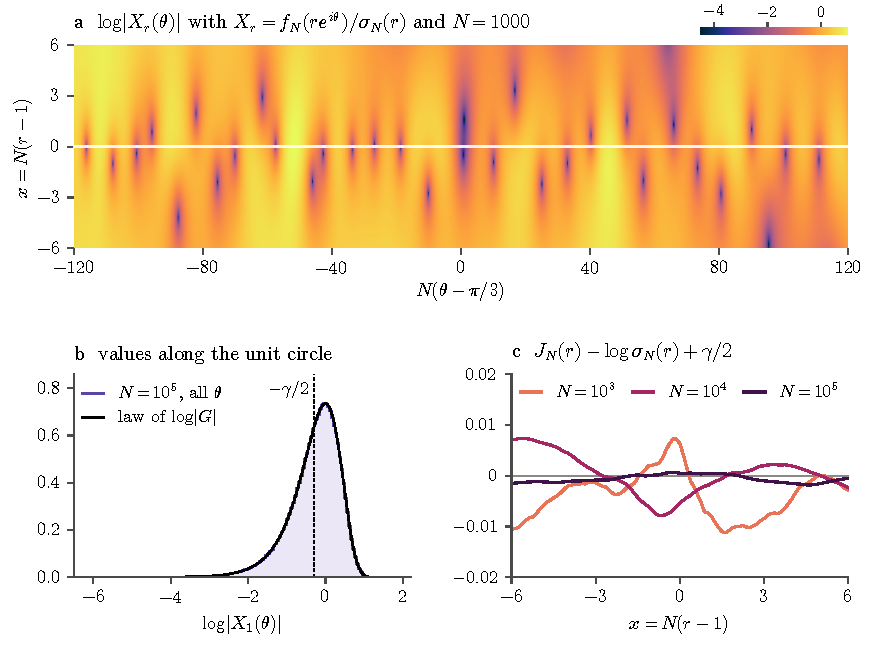
\includegraphics[width=\textwidth]{figures/explanatory/angular-logarithm.pdf}
\caption{The angular logarithm for one sequence near $e^{i\pi/3}$, with the
zeros as dark spots (a), its distribution (b), and its centered mean at
three degrees (c).}
\label{fig:angular-logarithm}
\end{figure}


\subsection{One- and two-point bounds}
\label{sec:h1-rademacher}
We show that, for radii $r,s\in[1-K/N,1+K/N]$ and for angles $\theta,\phi$
outside small exceptional sets, the probabilities that $X_r(\theta)$ lies
in a disk centered at $0$ and that $(X_r(\theta),X_s(\phi))$ lies in a
product of two such disks differ by $O_K(N^{-1/2})$ from those for one and
for two independent copies of $G$. Summation by parts shows that the
covariance matrices are close to $\tfrac12I$, Rai\v{c}'s theorem and an
interpolation of densities compare the laws with that of $G$, and we then
deduce bounds for the mean and the variance of the angular occupation of
a disk.

By the definition of $X_r$,
\[
 \begin{pmatrix}\Re X_r(\theta)\\ \Im X_r(\theta)\end{pmatrix}
 =\sum_{k=0}^N\epsilon_k\frac{r^k}{\sigma_N(r)}
 \begin{pmatrix}\cos(k\theta)\\ \sin(k\theta)\end{pmatrix}.
\]
Since the signs are independent with mean zero and variance one, the
covariance matrix of $(\Re X_r(\theta),\Im X_r(\theta))$ is given by
\[
 V(r,\theta)=\frac1{\sigma_N(r)^2}\sum_{k=0}^Nr^{2k}
 \begin{pmatrix}
 \cos^2(k\theta)&\cos(k\theta)\sin(k\theta)\\
 \cos(k\theta)\sin(k\theta)&\sin^2(k\theta)
 \end{pmatrix}.
\]
For two points, the covariance matrix of
$(\Re X_r(\theta),\Im X_r(\theta),\Re X_s(\phi),\Im X_s(\phi))$ is the
$4\times4$ matrix
\[
 \begin{pmatrix}
 V(r,\theta)&V(r,s,\theta,\phi)\\
 V(r,s,\theta,\phi)^T&V(s,\phi)
 \end{pmatrix},
\]
where
\[
 V(r,s,\theta,\phi)=\frac1{\sigma_N(r)\sigma_N(s)}\sum_{k=0}^N(rs)^k
 \begin{pmatrix}
 \cos(k\theta)\cos(k\phi)&\cos(k\theta)\sin(k\phi)\\
 \sin(k\theta)\cos(k\phi)&\sin(k\theta)\sin(k\phi)
 \end{pmatrix},
\]
so that $V(r,\theta)=V(r,r,\theta,\theta)$.
By the product-to-sum identities with $x,y\in\{k\theta,k\phi\}$, and
since $\sigma_N(r)^2=\sum_{k=0}^Nr^{2k}$, we get
\begin{align*}
 V(r,\theta)&=\frac12I_2+\frac1{2\sigma_N(r)^2}\sum_{k=0}^Nr^{2k}
 \begin{pmatrix}
 \cos(2k\theta)&\sin(2k\theta)\\
 \sin(2k\theta)&-\cos(2k\theta)
 \end{pmatrix},\\
 V(r,s,\theta,\phi)&=\frac1{2\sigma_N(r)\sigma_N(s)}\sum_{k=0}^N(rs)^k\\
 &\quad\times
 \begin{pmatrix}
 \cos(k(\theta-\phi))+\cos(k(\theta+\phi))&
 \sin(k(\theta+\phi))-\sin(k(\theta-\phi))\\
 \sin(k(\theta+\phi))+\sin(k(\theta-\phi))&
 \cos(k(\theta-\phi))-\cos(k(\theta+\phi))
 \end{pmatrix}.
\end{align*}
In terms of the rotation and the reflection
\begin{equation}
 R(\psi)=\begin{pmatrix}\cos\psi&-\sin\psi\\ \sin\psi&\cos\psi\end{pmatrix},
 \qquad
 F(\psi)=\begin{pmatrix}\cos\psi&\sin\psi\\ \sin\psi&-\cos\psi\end{pmatrix},
 \label{eq:rotation-reflection}
\end{equation}
the matrix summands are $F(2k\theta)$ and
$\Theta_k=R(k(\theta-\phi))+F(k(\theta+\phi))$, so that
\begin{align*}
 V(r,\theta)&=\frac12I_2+\frac1{2\sigma_N(r)^2}\sum_{k=0}^Nr^{2k}F(2k\theta),\\
 V(r,s,\theta,\phi)&=\frac1{2\sigma_N(r)\sigma_N(s)}\sum_{k=0}^N(rs)^k\Theta_k.
\end{align*}
The oscillatory sums are small unless $2\theta$, $2\phi$, $\theta-\phi$ or
$\theta+\phi$ is close to $2\pi\mathbb Z$, and we remove these angles.

For one point, we remove the set
$\operatorname{dist}(\theta,\pi\mathbb Z)<N^{-1/2}$: two arcs of length
$2N^{-1/2}$, of normalized measure
$4N^{-1/2}/(2\pi)=2N^{-1/2}/\pi\le2N^{-1/2}$. Every retained angle
satisfies
$\operatorname{dist}(2\theta,2\pi\mathbb Z)=2\operatorname{dist}(\theta,\pi\mathbb Z)\ge2N^{-1/2}$.
For two points, we remove this set in each coordinate, and the sets
$\operatorname{dist}(\theta\mp\phi,2\pi\mathbb Z)<N^{-1/2}$, each an arc of
$\theta$ of normalized length $N^{-1/2}/\pi$ for fixed $\phi$. The removed
part of the angular square has measure at most
$2N^{-1/2}+2N^{-1/2}+2N^{-1/2}/\pi\le10N^{-1/2}$.

The entries of these matrices are real and imaginary parts of weighted
exponential sums, which we bound by summation by parts.
Let $r,s\in[1-K/N,1+K/N]$, $N\ge2K$ and $\beta\in\{0,1,2\}$, and for
$\operatorname{dist}(\psi,2\pi\mathbb Z)>0$ set
\[
 b_k=(rs)^k(k/N)^\beta,\qquad S_\ell(\psi)=\sum_{k=0}^\ell e^{ik\psi},
\]
where $(k/N)^0=1$, including $k=0$, and $S_{-1}(\psi)=0$.
Summing the geometric series, and since
$|1-e^{i\psi}|=2|\sin(\psi/2)|\ge2\operatorname{dist}(\psi,2\pi\mathbb Z)/\pi$,
we get
\[
 S_\ell(\psi)=\frac{1-e^{i(\ell+1)\psi}}{1-e^{i\psi}},\qquad
 |S_\ell(\psi)|\le\frac2{|1-e^{i\psi}|}
 \le\frac\pi{\operatorname{dist}(\psi,2\pi\mathbb Z)}.
\]
Summation by parts yields
\[
 \sum_{k=0}^Nb_ke^{ik\psi}
 =\sum_{k=0}^Nb_k\bigl(S_k(\psi)-S_{k-1}(\psi)\bigr)
 =b_NS_N(\psi)+\sum_{k=0}^{N-1}(b_k-b_{k+1})S_k(\psi).
\]
For $\beta=0$ the weights are geometric. For $\beta>0$ we have $b_0=0$
and the ratios $b_{k+1}/b_k=(rs)(1+1/k)^\beta$, $k\ge1$, are
nonincreasing, so the weights first increase and then decrease (either
part may be empty). Let $b_*=\max_{k\le N}b_k$. The variation of such
weights is the rise from $b_0$ to $b_*$ plus the fall from $b_*$ to
$b_N$, and $b_k\le(rs)^k\le\max(1,rs)^N$ with $rs\le(1+K/N)^2$, so that
\begin{align*}
 b_*&\le(1+K/N)^{2N}\le e^{2K},\\
 \sum_{k=0}^{N-1}|b_{k+1}-b_k|&=2b_*-b_0-b_N,\\
 b_N+\sum_{k=0}^{N-1}|b_{k+1}-b_k|
 &\le b_0+b_N+2b_*\le4e^{2K}.
\end{align*}
Consequently, since $4\pi\le10e^{2K}$ for $K\ge2$,
\begin{equation}
 \begin{aligned}
 \left|N^{-1}\sum_{k=0}^N(rs)^k(k/N)^\beta e^{ik\psi}\right|
 &\le\frac\pi{N\operatorname{dist}(\psi,2\pi\mathbb Z)}
       \left(b_N+\sum_{k=0}^{N-1}|b_{k+1}-b_k|\right)\\
 &\le\frac{4\pi e^{2K}}{N\operatorname{dist}(\psi,2\pi\mathbb Z)}
 \le\frac{10e^{4K}}{N\operatorname{dist}(\psi,2\pi\mathbb Z)}.
 \end{aligned}                                      \label{eq:layer2-abel}
\end{equation}
We keep the larger constant $10e^{4K}$, from which the later bounds are
computed.

If $N\ge2K$ and $r\in[1-K/N,1+K/N]$, then each term of $\sigma_N(r)^2$
satisfies $e^{-4K}\le(1-K/N)^{2N}\le r^{2k}\le(1+K/N)^{2N}\le e^{2K}$,
since $\log(1-x)\ge-2x$ for $0\le x\le K/N\le1/2$. Summing the $N+1$
terms, we get the radial bounds
\begin{equation}
 Ne^{-4K}\le(N+1)e^{-4K}\le\sigma_N(r)^2\le(N+1)e^{2K}\le2Ne^{2K}.
 \label{eq:radial-bounds}
\end{equation}

The entries of $R(\psi)$ and $F(\psi)$ are $\pm\cos\psi$ and
$\pm\sin\psi$. Hence every entry of $V(r,\theta)-\tfrac12I_2$ is
$N/(2\sigma_N(r)^2)$ times $\pm$ the real or imaginary part of the sum in
\eqref{eq:layer2-abel} with $s=r$, $\beta=0$ and $\psi=2\theta$, and every
entry of $V(r,s,\theta,\phi)$ is $N/(2\sigma_N(r)\sigma_N(s))$ times the
sum of two such terms, with $\beta=0$ and $\psi=\theta\mp\phi$.
At the retained angles, by \eqref{eq:layer2-abel} and the lower bound in
\eqref{eq:radial-bounds}, these entries are at most, in absolute value,
\begin{equation}
 \begin{aligned}
 \frac N{2\sigma_N(r)^2}
 \left|\frac1N\sum_{k=0}^Nr^{2k}e^{2ik\theta}\right|
 &\le\frac{e^{4K}}2\cdot\frac{10e^{4K}}{N\cdot2N^{-1/2}}
 \le10e^{8K}N^{-1/2},\\
 \frac N{2\sigma_N(r)\sigma_N(s)}\sum_{\pm}
 \left|\frac1N\sum_{k=0}^N(rs)^ke^{ik(\theta\pm\phi)}\right|
 &\le\frac{e^{4K}}2\cdot2\cdot\frac{10e^{4K}}{N\cdot N^{-1/2}}
 =10e^{8K}N^{-1/2}.
 \end{aligned}\label{eq:covariance-entries}
\end{equation}
The first bound also holds for $V(s,\phi)-\tfrac12I_2$. The operator
norm of a $d\times d$ matrix is at most $d$ times its largest entry, so
at the retained angles $V(r,\theta)-\tfrac12I_2$ and the $4\times4$
covariance matrix minus $\tfrac12I_4$ have norm at most
$40e^{8K}N^{-1/2}$. From now on $N\ge(160e^{8K})^2$, so that this norm is
at most $1/4$ and every eigenvalue lies in $[1/4,3/4]$.

Rai\v{c}'s theorem \cite[Theorem 1.1]{Raic2019} states that, for
independent centered real vectors $Y_k$ with total covariance $I_d$ and a
measurable convex set $D$,
\[
 \left|\Prob\!\left(\sum_kY_k\in D\right)-\Prob(G_d\in D)\right|
 \le(42d^{1/4}+16)\sum_k\mathbb E\|Y_k\|^3,
\]
where $G_d$ is standard Gaussian in $\mathbb R^d$. For a covariance
matrix $\Sigma$ we write $G_\Sigma$ for a centered Gaussian vector with
covariance $\Sigma$, so that $G_d=G_{I_d}$; distances and entropies
between such vectors are those of their laws.
For two points, the summands and their covariance are
\[
 u_k=\begin{pmatrix}
 r^k\cos(k\theta)/\sigma_N(r)\\r^k\sin(k\theta)/\sigma_N(r)\\
 s^k\cos(k\phi)/\sigma_N(s)\\s^k\sin(k\phi)/\sigma_N(s)
 \end{pmatrix},\qquad
 \Sigma=\sum_{k=0}^Nu_ku_k^T,
\]
so that $\sum_{k=0}^N\epsilon_ku_k$ is the vector
$(\Re X_r(\theta),\Im X_r(\theta),\Re X_s(\phi),\Im X_s(\phi))^T$, whose
covariance $\Sigma$ is the $4\times4$ matrix above.
Let $Y_k=\epsilon_k\Sigma^{-1/2}u_k$. These are independent and centered,
since $\mathbb E\epsilon_k=0$ and $\mathbb E\epsilon_k^2=1$, and
$\|Y_k\|\le\|\Sigma^{-1/2}\|\|u_k\|\le2\|u_k\|$, since every eigenvalue of
$\Sigma$ is at least $1/4$. By $r^{2k},s^{2k}\le e^{2K}$ and the lower
bound in \eqref{eq:radial-bounds},
\begin{align*}
 \sum_{k=0}^N\mathbb E[Y_kY_k^T]
 &=\Sigma^{-1/2}\left(\sum_{k=0}^Nu_ku_k^T\right)\Sigma^{-1/2}
 =I_4,\\
 \|u_k\|^2
 &=\frac{r^{2k}}{\sigma_N(r)^2}+\frac{s^{2k}}{\sigma_N(s)^2}
 \le\frac{2e^{6K}}N,\\
 \sum_{k=0}^N\mathbb E\|Y_k\|^3
 &\le(N+1)\left(\frac{2\sqrt2e^{3K}}{\sqrt N}\right)^3
 \le32\sqrt2\,e^{9K}N^{-1/2}
 <46e^{9K}N^{-1/2}.
\end{align*}
For one point we use the first two coordinates, with
$\Sigma=V(r,\theta)$, and get the smaller bound
\[
 \|u_k\|^2=\frac{r^{2k}}{\sigma_N(r)^2}\le\frac{e^{6K}}N,\qquad
 \sum_{k=0}^N\mathbb E\|Y_k\|^3
 \le(N+1)\left(\frac{2e^{3K}}{\sqrt N}\right)^3
 \le16e^{9K}N^{-1/2}.
\]
Disks, products of disks and their images under whitening are
measurable and convex.

To compare $G_\Sigma$ with $G_{I_d/2}$, where $d=2$ or $4$, let
$\Delta=\Sigma-\tfrac12I_d$, so that $\|\Delta\|\le40e^{8K}N^{-1/2}\le1/4$,
and let $p_\lambda$ be the centered Gaussian
density with covariance $\Sigma_\lambda=\tfrac12I_d+\lambda\Delta$,
$0\le\lambda\le1$, whose eigenvalues lie in $[1/4,3/4]$. Then
\begin{align}
 \partial_\lambda p_\lambda(x)
 &=\frac{p_\lambda(x)}2\left\{
   x^T\Sigma_\lambda^{-1}\Delta\Sigma_\lambda^{-1}x-\operatorname{tr}(\Sigma_\lambda^{-1}\Delta)
   \right\},\nonumber\\
 \int_{\mathbb R^d}|\partial_\lambda p_\lambda(x)|\dd x
 &=\frac12\,\mathbb E\bigl|G_d^T\Sigma_\lambda^{-1/2}\Delta\Sigma_\lambda^{-1/2}G_d
   -\operatorname{tr}(\Sigma_\lambda^{-1/2}\Delta\Sigma_\lambda^{-1/2})\bigr|\nonumber\\
 &\le\frac{\sqrt{2d}}2\|\Sigma_\lambda^{-1/2}\Delta\Sigma_\lambda^{-1/2}\|
 \le2\sqrt{2d}\,\|\Delta\|,\nonumber\\
 \operatorname{TV}\bigl(G_\Sigma,G_{I_d/2}\bigr)
 &\le\frac12\int_0^1\int_{\mathbb R^d}|\partial_\lambda p_\lambda(x)|\dd x\dd\lambda
 \le\sqrt{2d}\,\|\Delta\|
 \le320e^{8K}N^{-1/2}.\label{eq:tv-circular}
\end{align}
The four lines of \eqref{eq:tv-circular} hold for these reasons.
\begin{enumerate}
\item The derivative uses
$\partial_\lambda\log\det\Sigma_\lambda=\operatorname{tr}(\Sigma_\lambda^{-1}\Delta)$
and
$\partial_\lambda\Sigma_\lambda^{-1}=-\Sigma_\lambda^{-1}\Delta\Sigma_\lambda^{-1}$.
\item The change of variables $x\mapsto\Sigma_\lambda^{-1/2}x$ carries
$p_\lambda$ to the law of $G_d$.
\item In an eigenbasis of $\Sigma_\lambda^{-1/2}\Delta\Sigma_\lambda^{-1/2}$,
with eigenvalues $a_1,\ldots,a_d$, the quadratic form minus the trace is
$\sum_ia_i(g_i^2-1)$ with independent standard real Gaussian $g_i$. It has
mean zero and variance
$2\sum_ia_i^2\le2d\|\Sigma_\lambda^{-1/2}\Delta\Sigma_\lambda^{-1/2}\|^2$,
so by Cauchy--Schwarz its mean absolute value is at most $\sqrt{2d}$ times
this norm, which is at most $4\|\Delta\|$ since
$\|\Sigma_\lambda^{-1}\|\le4$.
\item Total variation is half the $L^1$ distance,
$p_1-p_0=\int_0^1\partial_\lambda p_\lambda\dd\lambda$, and
$\sqrt{2d}\le2\sqrt2\le8$ for $d\le4$.
\end{enumerate}
The same computation gives, for positive-definite $\Sigma_0,\Sigma_1$ in
dimension $d$ such that every $\Sigma_0+\lambda(\Sigma_1-\Sigma_0)$,
$0\le\lambda\le1$, has least eigenvalue at least $\mu>0$,
$\operatorname{TV}(G_{\Sigma_1},G_{\Sigma_0})\le\sqrt{2d}\,\|\Sigma_1-\Sigma_0\|/(4\mu)$,
since the norm of $\Sigma_\lambda^{-1/2}(\Sigma_1-\Sigma_0)\Sigma_\lambda^{-1/2}$
is at most $\|\Sigma_1-\Sigma_0\|/\mu$.

Let $F_G(t)=\Prob(|G|\le t)=1-e^{-t^2}$, and for $t,t'\ge0$ let $D$ be
the disk $\{x\in\mathbb R^2:x_1^2+x_2^2\le t^2\}$ when $d=2$ and the
product of disks
$\{x\in\mathbb R^4:x_1^2+x_2^2\le t^2,\ x_3^2+x_4^2\le t'^2\}$ when $d=4$.
Since $\sum_k\epsilon_ku_k=\Sigma^{1/2}\sum_kY_k$ and $\Sigma^{1/2}G_d$
has the law of $G_\Sigma$, we have
$\Prob(\sum_k\epsilon_ku_k\in D)=\Prob(\sum_kY_k\in\Sigma^{-1/2}D)$ and
$\Prob(G_\Sigma\in D)=\Prob(G_d\in\Sigma^{-1/2}D)$. Hence, by Rai\v{c}'s
theorem with the third-moment bounds above and by \eqref{eq:tv-circular},
at retained angles and pairs,
\begin{align}
 &\bigl|\Prob\bigl(\textstyle\sum_k\epsilon_ku_k\in D\bigr)-\Prob(G_{I_d/2}\in D)\bigr|
 \nonumber\\
 &\qquad\le\bigl|\Prob\bigl(\textstyle\sum_kY_k\in\Sigma^{-1/2}D\bigr)
     -\Prob(G_d\in\Sigma^{-1/2}D)\bigr|
 +\bigl|\Prob(G_\Sigma\in D)-\Prob(G_{I_d/2}\in D)\bigr|
 \nonumber\\
 &\qquad\le(42d^{1/4}+16)\cdot46e^{9K}N^{-1/2}+320e^{8K}N^{-1/2}
 \le C(K)N^{-1/2}.\label{eq:point-bounds}
\end{align}
For $d=4$ the left-hand side is
$|\Prob(|X_r(\theta)|\le t,|X_s(\phi)|\le t')-F_G(t)F_G(t')|$, since the
two coordinate pairs of $G_{I_4/2}$ are independent copies of $G$, and
for $d=2$ it is $|\Prob(|X_r(\theta)|\le t)-F_G(t)|$.

Let $A_t=\mu\{\theta:|X_r(\theta)|\le t\}$ be the angular occupation.
By Tonelli's theorem,
\begin{align*}
 \mathbb EA_t&=\int\Prob(|X_r(\theta)|\le t)\dd\mu(\theta),\\
 \mathbb EA_t^2&=\int\!\!\int
   \Prob(|X_r(\theta)|\le t,|X_r(\phi)|\le t)\dd\mu(\theta)\dd\mu(\phi).
\end{align*}
On the removed sets, of measures at most $2N^{-1/2}$ and $10N^{-1/2}$, the
integrands differ from $F_G(t)$ and $F_G(t)^2$ by at most one; elsewhere
we use \eqref{eq:point-bounds}, with $s=r$ and $t'=t$ for the pairs.
Hence, uniformly for $t\ge0$, since $0\le\mathbb EA_t+F_G(t)\le2$,
\begin{align}
 |\mathbb EA_t-F_G(t)|&\le2N^{-1/2}+C(K)N^{-1/2}\le C(K)N^{-1/2},\nonumber\\
 |\mathbb EA_t^2-F_G(t)^2|&\le10N^{-1/2}+C(K)N^{-1/2}\le C(K)N^{-1/2},\nonumber\\
 \operatorname{Var}(A_t)
 &=\mathbb EA_t^2-F_G(t)^2-(\mathbb EA_t-F_G(t))(\mathbb EA_t+F_G(t))
 \nonumber\\
 &\le|\mathbb EA_t^2-F_G(t)^2|
       +|\mathbb EA_t-F_G(t)|\,|\mathbb EA_t+F_G(t)|
 \le C(K)N^{-1/2}.\label{eq:occupation-bounds}
\end{align}
The two-point argument also permits different radii and different disk
thresholds.

\subsection{Logarithmic integrability and angular energy}\label{sec:log-integrability}
The normalized Fourier coefficients satisfy
$\sum_{k=0}^N|r^k/\sigma_N(r)|^2=1$, which is the normalization in
$L^2(\Omega\times\mathbb T)$ of Corollary~1.2 of Nazarov--Nishry--Sodin
\cite{NNS2013}. By that corollary,
\begin{equation}
 \mathbb E\int |\log|X_r||^p\dd\mu\le(C_*p)^{6p},\qquad p\ge1,
                                                        \label{eq:layer2-nns}
\end{equation}
where $C_*\ge1$ is an absolute constant; zeros on the circle give only
integrable logarithmic singularities. By Parseval's identity, for every
choice of signs, the angular energy is
\begin{equation}
 \int|X_r|^2\dd\mu=\frac1{\sigma_N(r)^2}\sum_{k=0}^N\epsilon_k^2r^{2k}=1.
                                                        \label{eq:layer2-energy}
\end{equation}

We clip the logarithm at $\pm T$, control the clipped integral by the
occupation bounds, and control the two tails by the logarithmic moments
and the angular energy. Table~\ref{tab:clipping-level} lists what depends
on $T$.
\begin{table}[ht]
\centering
\small
\setlength{\tabcolsep}{4pt}
\begin{tabular}{@{}llll@{}}
\toprule
Quantity & Bound & At $T=c\log N$ & Requirement\\
\midrule
Gaussian mass of $\{|z|\le e^{-T}\}$ & $F_G(e^{-T})\le e^{-2T}$ & $N^{-2c}$ & tends to zero\\
Chebyshev bound for $A_{e^{-T}}$ & $C(K)N^{-1/2}e^{4T}$ & $C(K)N^{4c-1/2}$ & summable in $j$\\
Lower tail ($e^{-2T}\ge N^{-1/2}$) & order $(\log N)^7e^{-2T}$ & $(\log N)^7N^{-2c}$ & tends to zero\\
\bottomrule
\end{tabular}
\caption{The quantities in Lemma~\ref{lem:clipping} that depend on the
clipping level $T=c\log N$, for signs; the last row needs $c\le1/4$.
At $N=j^8$ the second is $C(K)j^{32c-4}$, summable when $c<3/32$.}
\label{tab:clipping-level}
\end{table}
Any $c$ in $(0,3/32)$ would do. By H\"older's inequality in
Theorem~\ref{thm:T1} the lower tail is of order $e^{-2T}$, up to the
logarithmic factor, so a larger $c$ gives a smaller error and a larger
failure probability. We take $c=1/32$: then $T=(1/32)\log N$,
$e^{-2T}=N^{-1/16}\ge N^{-1/2}$, the lower tail is
$(\log N)^7N^{-1/16}$, the error term of
Theorem~\ref{thm:sign-logarithms}, and
$N^{-1/2}e^{4T}=N^{-3/8}$, which is $j^{-3}$ at $N=j^8$. This failure
probability stays summable when $C(K)$ grows like a small power of $N$,
as in Section~\ref{sec:log-rate}.
We state the argument for coefficients that need not be signs, for use in
Section~\ref{sec:layer2-models}.

Theorem~\ref{thm:T1}, which we apply below, uses two facts about the
standard complex Gaussian variable $G$. For every $T\ge0$, since
$F_G(e^{-\tau})\le e^{-2\tau}$ and
$\Prob(|G|>e^\tau)\le e^{-2\tau}\mathbb E|G|^2=e^{-2\tau}$,
\begin{equation}
 \int_T^\infty\Prob(|G|<e^{-\tau})\dd\tau\le\tfrac12e^{-2T},\qquad
 \int_T^\infty\Prob(|G|>e^\tau)\dd\tau\le\tfrac12e^{-2T}.
 \label{eq:gaussian-log-tails}
\end{equation}
Since $|G|^2$ has the exponential distribution with mean one, the
classical integral for Euler's constant gives
\begin{equation}
 \mathbb E\log|G|=\frac12\,\mathbb E\log(|G|^2)
 =\frac12\int_0^\infty e^{-y}\log y\dd y
 =-\frac\gamma2.
 \label{eq:euler-centering}
\end{equation}

\begin{lemma}[Clipping]\label{lem:clipping}
Let $N\ge e$ and $r>0$, and let $X_r$ and $A_t$ be defined as above for a
random polynomial $f_N$ whose coefficients need not be signs.
Let $H\ge0$, $C>0$ and $B_E>0$ be constants and $E$ an event such that,
for all $t\ge0$ and $p\ge1$,
\begin{gather*}
 |\mathbb EA_t-F_G(t)|\le HN^{-1/2},\qquad
 \operatorname{Var}(A_t)\le HN^{-1/2},\\
 \int_E\int|\log|X_r||^p\dd\mu\dd\Prob\le(Cp)^{6p},
\end{gather*}
and $\int|X_r|^2\dd\mu\le B_E$ on $E$. Let $T=(1/32)\log N$ and
\begin{align*}
 \varepsilon&=N^{-1/16}(\log N)^7+2HTN^{-1/2}\\
 &\quad+e^{1/2}(4eC)^6(2N^{-1/16}+HN^{-1/2})(\log N)^7+(B_E/2+1)N^{-1/16}\\
 &\le\bigl(2+2e^{1/2}(4eC)^6+B_E/2\bigr)N^{-1/16}(\log N)^7\\
 &\quad+\bigl(\tfrac1{16}+e^{1/2}(4eC)^6\bigr)HN^{-1/2}(\log N)^7.
\end{align*}
Then
\begin{align*}
 &\Prob\{|J_N(r)-\log\sigma_N(r)+\gamma/2|>\varepsilon\}\\
 &\qquad\le HN^{-3/8}+N^{-12}+\frac{H}{256}N^{-3/8}(\log N)^{-12}
 +\Prob(E^c).
\end{align*}
\end{lemma}

\begin{proof}
This is Theorem~\ref{thm:T1} in the variant form given at the end of its
statement, with $X=X_r$,
$d_1=v=HN^{-1/2}$, $\beta=6$, $E_H=E$, $T=(1/32)\log N$,
$u=N^{-1/16}(\log N)^7$, $b=N^{-1/16}$, $q=\lceil\log N\rceil$ and
$\lambda=(2e\log N/q)^6\log N$. Its hypotheses hold, since the
occupation bounds of the lemma are the bounds on $\mathbb EA_t$ and
$\operatorname{Var}(A_t)$ of that form, the moment bound of the lemma
is \eqref{eq:event-log-moment-bound} with $E_H=E$ and $\beta=6$, and
$\int|X_r|^2\dd\mu\le B_E$ on $E$.
For $N\ge e$ we have $\log N\le q\le\log N+1\le2\log N$, so that
$\lambda\ge e^6\log N>1$,
\[
 \lambda(2Cq)^6
 =\Bigl(\frac{2e\log N}q\Bigr)^6(\log N)(2Cq)^6
 =(4eC)^6(\log N)^7
\]
and
\[
 \lambda^{-2q}
 =\left[\left(\frac q{2e\log N}\right)^{12}(\log N)^{-2}\right]^q
 \le\bigl[e^{-12}(\log N)^{-2}\bigr]^q
 \le N^{-12},
\]
where the last two steps use $q\le2\log N$, $\log N\ge1$ and
$q\ge\log N$. By the first identity, the Markov event for $W$ in the
proof of Theorem~\ref{thm:T1} is
$E\cap\{W>((4eC)^6(\log N)^7)^{2q}\}$, where
$W=\int|\log|X_r||^{2q}\dd\mu$.
Since $e^{-2T}=b=N^{-1/16}$, the base
$x=e^{-2T}+d_1+b=2N^{-1/16}+HN^{-1/2}$ satisfies $x\ge N^{-1}$, and
hence $x^{-1/(2q)}\le N^{1/(2q)}\le e^{1/2}$, since $q\ge\log N$, so that
\[
 x^{1-1/(2q)}\le e^{1/2}x=e^{1/2}(2N^{-1/16}+HN^{-1/2}),
\]
and the error $\eta_{\log}$ of \eqref{eq:T1-error} is at most
$\varepsilon$. The first three terms of \eqref{eq:T1-failure} are
$v/b^2=HN^{-1/2}N^{1/8}=HN^{-3/8}$, $\lambda^{-2q}\le N^{-12}$ and
$4T^2v/u^2=4HT^2N^{-3/8}(\log N)^{-14}=(H/256)N^{-3/8}(\log N)^{-12}$,
since $4T^2=(\log N)^2/256$, and $p_E+p_H$ is replaced by
$\Prob(E^c)$.
Since $J_N(r)-\log\sigma_N(r)=\int\log|X_r|\dd\mu$ and
$\mathbb E\log|G|=-\gamma/2$ by \eqref{eq:euler-centering}, this is the
bound of the lemma. The bound on $\varepsilon$ in the statement uses
$2TN^{-1/2}=\frac1{16}N^{-1/2}\log N\le\frac1{16}N^{-1/2}(\log N)^7$ and
$N^{-1/16}\le N^{-1/16}(\log N)^7$ for $N\ge e$, and keeps the terms with
$H$, which carry the factor $N^{-1/2}$, apart from the others.
\end{proof}

\begin{proof}[Proof of Theorem~\ref{thm:sign-logarithms}]
By \eqref{eq:occupation-bounds}, \eqref{eq:layer2-nns} and
\eqref{eq:layer2-energy}, Lemma~\ref{lem:clipping} applies with $H$ the
constant $C(K)$ of \eqref{eq:occupation-bounds}, $C=C_*$, $E=\Omega$ and
$B_E=1$.
Since $C_*$ is an absolute constant and $N^{-1/2}\le N^{-1/16}$, its
error $\varepsilon$ is at most $C(K)N^{-1/16}(\log N)^7$, and, since
$\Prob(E^c)=0$, its probability
bound is at most the right-hand side of
\eqref{eq:sign-log-concentration}.
All constants above depend only on $K$, and all bounds hold uniformly
for $r\in[1-K/N,1+K/N]$.
\end{proof}

\subsection{Radial mass and thin bands with high probability}

\begin{corollary}[Annular mass and thin bands]\label{cor:radial-probability}
Fix $K\ge2$ and $0<\kappa\le1/64$, and take $N$ sufficiently large.
Outside four events, each of probability at most the right-hand side of
\eqref{eq:sign-log-concentration},
\begin{equation}
 \frac{\#\{\alpha:||\alpha|-1|>K/N\}}N
 \le\frac{2\log2}{K}+C(K)N^{-1/16}(\log N)^7.
                                                        \label{eq:sign-annular-mass}
\end{equation}
Outside five further events of the same kind, for
$q=-1,0,1$,
\begin{equation}
 \left|\frac{\nu_N(1+qN^{-1-\kappa})}N-\frac12\right|
 \le2N^{-\kappa}+C(K)N^{\kappa-1/16}(\log N)^7.
                                                        \label{eq:sign-thin-band}
\end{equation}
\end{corollary}

By Theorem~\ref{thm:sign-logarithms}, the sum of the probabilities of
these nine exceptional events is summable at $N=j^8$.

\begin{proof}
We apply the deterministic Lemmas~\ref{lem:annular-mass}
and~\ref{lem:thin-band} outside the exceptional events of
Theorem~\ref{thm:sign-logarithms} at their radii; $f_N\ne0$ since
$f_N(0)=\epsilon_0\ne0$.

The four secant radii $r_i=1+x_i/N$ of Lemma~\ref{lem:annular-mass} with
$\eta=1/2$ lie in $[1-K/N,1+K/N]$. Outside the four logarithmic
exceptional events at these radii, the first hypothesis of that lemma
holds with $\varepsilon=C(K)N^{-1/16}(\log N)^7$, by
Theorem~\ref{thm:sign-logarithms}, and the second with
$D=K^2+e^{4K}/2$, by Lemma~\ref{lem:profile-rate}, since $|x_i|\le K$
and $N\ge2K$.
Therefore Lemma~\ref{lem:annular-mass} at $\eta=1/2$ and
$1/N\le N^{-1/16}(\log N)^7$, for $N\ge3$, yield
\begin{align*}
 \frac{\#\{\alpha:||\alpha|-1|>K/N\}}N
 &\le\frac{2\log2}K+\frac8K\Big(C(K)N^{-1/16}(\log N)^7
       +\frac{K^2+e^{4K}/2}N\Big)\\
 &\le\frac{2\log2}K+\frac8K\Big(C(K)+K^2+\frac{e^{4K}}2\Big)
       N^{-1/16}(\log N)^7\\
 &\le\frac{2\log2}{K}+C(K)N^{-1/16}(\log N)^7,
\end{align*}
which is \eqref{eq:sign-annular-mass}.

The five radii $1+qN^{-1-\kappa}$, $q=-2,\dots,2$, lie in the same
annulus, since $|qN^{-1-\kappa}|\le2N^{-1-\kappa}\le K/N$.
Outside the five logarithmic exceptional events at these radii,
Lemma~\ref{lem:thin-band} applies with
$\varepsilon=C(K)N^{-1/16}(\log N)^7$ (and $N\ge4$), and bounds the
left-hand side of \eqref{eq:sign-thin-band} by
$2N^{-\kappa}+4C(K)N^{-1/16}(\log N)^7N^{\kappa}
=2N^{-\kappa}+4C(K)N^{\kappa-1/16}(\log N)^7$.
Both terms tend to zero, since $\kappa\le1/64<1/16$.
\end{proof}

Figure~\ref{fig:annulus} compares the fraction of roots outside the
annulus with $2\log2/K$, the part of \eqref{eq:sign-annular-mass} that
does not tend to zero.
Panel (a) also shows the limit $1-\{\Phi(K)-\Phi(-K)\}$ of the fraction,
and panel (b) shows $K$ times its difference from this limit, with
pointwise 95\% bootstrap bands, both over 77 sequences.

\begin{figure}[t]
\centering
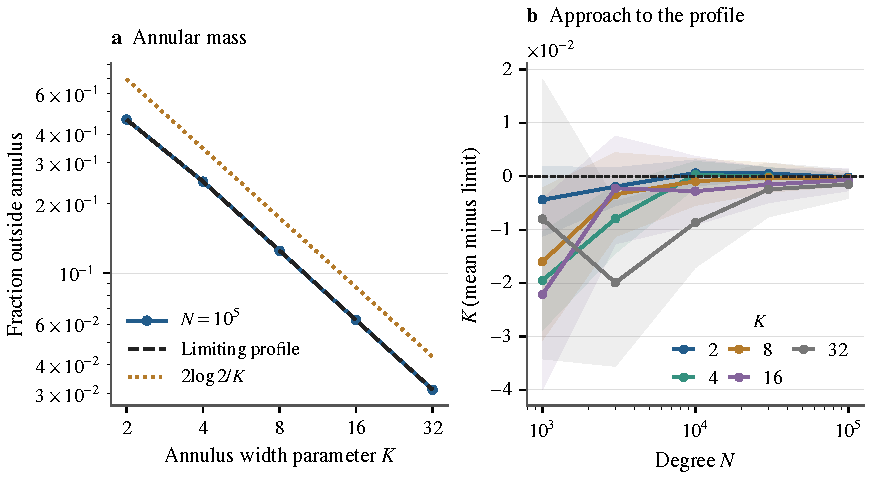
\includegraphics[width=\textwidth]{../numerics/publication/figures/annulus.pdf}
\caption{The fraction of zeros outside the annulus of width $K/N$.}
\label{fig:annulus}
\end{figure}


\section{Local zeros and small derivatives}
\label{sec:local-roots}
\subsection{Local zero counts}\label{sec:local-root-count}
We will use the Hanson--Wright inequality of Rudelson--Vershynin
\cite[Theorem 1.1]{RudelsonVershynin2013}: if $\xi$ is a random vector
with independent centered real coordinates whose
$\psi_2$ norm is at most $\Lambda$, $M$ is a real matrix and $t>0$, then
\[
 \Prob\{|\xi^TM\xi-\mathbb E\xi^TM\xi|>t\}
 \le2\exp\left[-c_{\rm HW}\min\left\{
 \frac{t^2}{\Lambda^4\|M\|_{\rm HS}^2},\frac{t}{\Lambda^2\|M\|}\right\}\right],
\]
where $c_{\rm HW}>0$ is an absolute constant.
Rudelson and Vershynin use the moment convention for $\psi_2$, and signs
satisfy both it and the equivalent exponential-moment convention with
$\Lambda=2$, since $p^{-1/2}(\mathbb E|\epsilon_k|^p)^{1/p}=p^{-1/2}\le2$
for $p\ge1$ and $\mathbb E\exp(\epsilon_k^2/2^2)=e^{1/4}\le2$.
Hence, for independent uniform signs $\epsilon=(\epsilon_0,\dots,\epsilon_N)$,
a real $(N+1)\times(N+1)$ matrix $M$ and $t>0$,
\begin{equation}
 \Prob\{|\epsilon^TM\epsilon-\mathbb E\epsilon^TM\epsilon|>t\}
 \le2\exp\left[-c_{\rm HW}\min\left\{
 \frac{t^2}{16\|M\|_{\rm HS}^2},\frac{t}{4\|M\|}\right\}\right].
 \label{eq:HW-signs}
\end{equation}

We first bound the local zero counts when the coefficients are independent
signs times bounded amplitudes, and then we specialize this bound to signs.

\begin{lemma}[Local zero counts for bounded amplitudes]
\label{lem:local-counts-general}
Fix $K\ge2$, $B\ge1$ and $\tfrac12\le\eta\le1$, and put
\[
 A(B,\eta)=\max\left(1,\frac{1024\pi B^2}{c_{\rm HW}\eta}\right),\qquad
 t_N(B,\eta)=\frac{A(B,\eta)\log N}{N},
\]
\[
 C_1(K,B,\eta)=\frac{4A(B,\eta)+4K+4+\log B}{\log2}.
\]
Let $N\ge e$ with $t_N(B,\eta)\le1$.
Let $\epsilon_0,\dots,\epsilon_N$ be independent uniform signs, and let
$a_0,\dots,a_N$ be real or complex random variables, independent of the
signs, with $|a_k|\le B$ for every $k$.
Let $\mathcal E$ be an event determined by $a_0,\dots,a_N$ on which
\[
 \sum_{k=0}^N|a_k|^2\ge\eta(N+1),
\]
and put $P_N(z)=\sum_{k=0}^N\epsilon_ka_kz^k$.
Then the probability that $\mathcal E$ occurs and some disk
\[
 \{z:|z-z_0|\le2K/N\},\qquad ||z_0|-1|\le1/N,
\]
contains more than $C_1(K,B,\eta)\log N$ zeros of $P_N$ is at most $N^{-3}$.
\end{lemma}

\begin{proof}
The idea is to show that the mean of $|P_N|^2$ over each arc of a fine
angular grid is at least half its conditional expectation, and then to
apply Jensen's formula at a point of the arc at which $|P_N|$ is large.

We condition on $a_0,\dots,a_N$ and assume that $\mathcal E$ occurs, so
that the signs remain independent and uniform. We take
$J=\lceil2\pi/t_N(B,\eta)\rceil$ equally spaced angular centers, with the
closed arc of radian length $2t_N(B,\eta)$ around each center.
Since $t_N(B,\eta)\le1<\pi$, every such arc $I$ has
$\mu(I)=t_N(B,\eta)/\pi$, and since $A(B,\eta)\ge1$ and $\log N\ge1$,
\[
 J\le\frac{2\pi}{t_N(B,\eta)}+1=\frac{2\pi N}{A(B,\eta)\log N}+1
 \le2\pi N+1\le8N.
\]
For each such arc $I$, the conditional real Gram matrix is defined by
\[
 (A_I)_{jk}=\int_I\Re\bigl(a_j\overline{a_k}e^{i(j-k)\theta}\bigr)\dd\mu(\theta),
 \qquad 0\le j,k\le N.
\]
For every real vector $x$, since the $x_k$ are real and by Parseval's
identity on the whole circle, we have
\begin{align*}
 0\le x^TA_Ix
 &=\int_I\left|\sum_{k=0}^Nx_ka_ke^{ik\theta}\right|^2\dd\mu(\theta)
 \le\int\left|\sum_{k=0}^Nx_ka_ke^{ik\theta}\right|^2\dd\mu(\theta)\\
 &=\sum_{k=0}^Nx_k^2|a_k|^2\le B^2\|x\|^2.
\end{align*}
It follows that the eigenvalues of the real symmetric matrix $A_I$ lie in
$[0,B^2]$, and since they are nonnegative, we have
\begin{gather*}
 \|A_I\|\le B^2,\qquad
 \|A_I\|_{\rm HS}^2\le\|A_I\|\operatorname{tr}A_I\le B^2\operatorname{tr}A_I,\\
 \operatorname{tr}A_I=\mu(I)\sum_{k=0}^N|a_k|^2\ge\eta(N+1)\mu(I)
 =\frac{\eta(N+1)t_N(B,\eta)}{\pi},
\end{gather*}
where the trace identity follows from $(A_I)_{kk}=|a_k|^2\mu(I)$, and the
inequality after it from $\mathcal E$.
Taking $x=\epsilon$ in the identity above and using
$\mathbb E\epsilon_j\epsilon_k=\mathbf 1\{j=k\}$, we obtain
\[
 Q_I:=\int_I|P_N(e^{i\theta})|^2\dd\mu(\theta)=\epsilon^TA_I\epsilon,\qquad
 \mathbb E_\epsilon Q_I=\operatorname{tr}A_I.
\]
If $Q_I<\tfrac12\operatorname{tr}A_I$, then
$|Q_I-\mathbb E_\epsilon Q_I|>\tfrac12\operatorname{tr}A_I$.
By \eqref{eq:HW-signs} with $M=A_I$ and $t=\tfrac12\operatorname{tr}A_I$,
and the bounds above, we have
\begin{align*}
 \Prob_\epsilon\{Q_I<\tfrac12\operatorname{tr}A_I\}
 &\le2\exp\left[-c_{\rm HW}\min\left\{
   \frac{(\operatorname{tr}A_I)^2}{64\|A_I\|_{\rm HS}^2},
   \frac{\operatorname{tr}A_I}{8\|A_I\|}\right\}\right]\\
 &\le2\exp\left[-c_{\rm HW}\min\left\{
   \frac{\operatorname{tr}A_I}{64B^2},
   \frac{\operatorname{tr}A_I}{8B^2}\right\}\right]
 =2\exp\left[-\frac{c_{\rm HW}\operatorname{tr}A_I}{64B^2}\right]\\
 &\le2\exp\left[-\frac{c_{\rm HW}\eta(N+1)A(B,\eta)\log N}{64\pi B^2N}\right]
 \le2e^{-16\log N}=2N^{-16},
\end{align*}
where the last inequality holds since
$A(B,\eta)\ge1024\pi B^2/(c_{\rm HW}\eta)$.
By the union bound over the at most $8N$ arcs, we get
\[
 \Prob_\epsilon\{Q_I<\tfrac12\operatorname{tr}A_I
 \text{ for some arc }I\}
 \le(8N)(2N^{-16})=16N^{-15}\le N^{-3}.
\]
Taking the expectation over $a_0,\dots,a_N$ on $\mathcal E$, we see that
the probability that $\mathcal E$ occurs and some arc has
$Q_I<\tfrac12\operatorname{tr}A_I$ is at most $N^{-3}$.

It remains to bound the number of zeros when $\mathcal E$ occurs and
every arc has $Q_I\ge\tfrac12\operatorname{tr}A_I$.
In this case, averaging over each closed arc and using the lower bound on
$\operatorname{tr}A_I$, we get
\[
 \max_{\theta\in I}|P_N(e^{i\theta})|^2\ge\frac{Q_I}{\mu(I)}
 \ge\frac{\operatorname{tr}A_I}{2\mu(I)}\ge\frac{\eta(N+1)}2.
\]
By continuity, there exists $z_1=e^{i\theta_1}$ on the arc such that
$|P_N(z_1)|^2\ge\eta(N+1)/2$.
Now let $||z_0|-1|\le1/N$.
Then the angular center nearest to $z_0/|z_0|$ is at angular distance at
most $\pi/J\le t_N(B,\eta)/2$ from it, and such a point $z_1$ on its arc
is at angular distance at most $t_N(B,\eta)$ from the center, so that
$|z_0/|z_0|-z_1|\le3t_N(B,\eta)/2$, since a chord is at most its arc.
Let $R=(2K+1)/N+2t_N(B,\eta)$. For $|z-z_0|\le2K/N$, since
$\bigl|z_0-z_0/|z_0|\bigr|=||z_0|-1|\le1/N$, we have
\[
 |z-z_1|\le|z-z_0|+\bigl|z_0-z_0/|z_0|\bigr|+\bigl|z_0/|z_0|-z_1\bigr|
 \le\frac{2K}N+\frac1N+\frac{3t_N(B,\eta)}2<R,
\]
so that the target disk lies strictly within $\{|z-z_1|<R\}$.
For $|z-z_1|\le2R$ we have $|z|\le1+2R$, and hence
\[
 |P_N(z)|\le\sum_{k=0}^N|a_k||z|^k\le B(N+1)(1+2R)^N\le B(N+1)e^{2NR}.
\]
Let $n(s)$ denote the number of zeros of $P_N$ in $|z-z_1|\le s$.
Since $P_N(z_1)\ne0$, Jensen's formula applies on the disk $|z-z_1|\le2R$,
and using $2NR=4K+2+4A(B,\eta)\log N$ we get
\begin{align*}
 &\#\{\alpha:|\alpha-z_1|<R\}
 \le n(R)\le\frac1{\log2}\int_R^{2R}\frac{n(s)}s\dd s\\
 &\qquad\le\frac{\max_{|z-z_1|=2R}\log|P_N(z)|-\log|P_N(z_1)|}{\log2}\\
 &\qquad\le\frac{\log\bigl(B(N+1)e^{2NR}\bigr)
   -\tfrac12\log\bigl(\eta(N+1)/2\bigr)}{\log2}\\
 &\qquad=\frac{\tfrac12\log(N+1)+\log B+\tfrac12\log(2/\eta)+2NR}{\log2}\\
 &\qquad=\frac{\tfrac12\log(N+1)+\log B+\tfrac12\log(2/\eta)
   +4K+2+4A(B,\eta)\log N}{\log2}\\
 &\qquad\le\frac{\log N+(4K+3+\log B)\log N+4A(B,\eta)\log N}{\log2}
 =C_1(K,B,\eta)\log N.
\end{align*}
The second inequality is the zero-count step of
\cite[\S8.21]{Titchmarsh1939}, the third is Jensen's formula
\cite[\S3.61]{Titchmarsh1939} for $P_N(z_1+z)$, and the last uses
$\tfrac12\log(N+1)\le\log N$ for $N\ge2$,
$\tfrac12\log(2/\eta)\le\tfrac12\log4=\log2$ for $\eta\ge\tfrac12$, and
$\log B+\log2+4K+2\le(4K+3+\log B)\log N$, which holds for
$\log N\ge1$ since $\log B\ge0$ and $\log2<1$.
Since the containment is strict, this count includes the zeros on the
boundary of the target disk, and since the angular cover is finite and
does not depend on $z_0$, the bound holds for every admissible center
$z_0$ at once.
\end{proof}

\begin{lemma}[Local zero counts]\label{lem:local-counts}
Fix $K\ge2$ and take $N$ sufficiently large.
Except on an event of probability at most $N^{-3}$, every disk
\[
 \{z:|z-z_0|\le2K/N\},\qquad ||z_0|-1|\le1/N,
\]
contains at most $C(K)\log N$ zeros of $f_N$.
\end{lemma}

The local-count constant is computed in Section~\ref{app:const-local}.

\begin{proof}
We apply Lemma~\ref{lem:local-counts-general} with $a_k=1$ for every $k$,
$B=1$, $\eta=1$ and $\mathcal E=\Omega$, which we may do since
$\sum_{k=0}^N|a_k|^2=N+1$.
Then $P_N=f_N$, and since $\log1=0$, the constants of that lemma are
\begin{align*}
 A(1,1)&=\max(1,1024\pi/c_{\rm HW})=A,\qquad
 t_N(1,1)=\frac{A\log N}N=t_N,\\
 C_1(K,1,1)&=\frac{4A+4K+4}{\log2}=C_1(K),
\end{align*}
which are the constants of Section~\ref{app:const-local}.
The conditions $N\ge e$ and $t_N\le1$ hold for all sufficiently large
$N$, since $t_N\to0$.
This proves the lemma with $C(K)=C_1(K)$.
\end{proof}

\subsection{Derivative detection and small-ball estimates}\label{sec:derivative-detection}
In this subsection we fix $K\ge2$, let $L=N^{1/64}$, and consider the
annulus $||z|-1|\le K/N$.

\begin{lemma}[Second derivative]\label{lem:second-derivative}
For every $N\ge\max\{2,(K+1)/3\}$, outside an event of probability at most
$N^{-10}$,
\begin{equation}
 \sup_{|z|\le1+(K+1)/N}|f_N''(z)|
 \le C(K)N^{5/2}\sqrt{\log N},
                                                        \label{eq:sign-second-derivative}
\end{equation}
and one can take $C(K)=100e^{K+4}$.
\end{lemma}

\begin{proof}
We first bound $f_N''$ at finitely many points of the circle
$|z|=1+(K+1)/N$ by Hoeffding's inequality, then pass to the whole circle
using a deterministic bound on $f_N'''$, and finally to the disk by the
maximum principle.
Bounds of this order for the supremum of a random trigonometric
polynomial go back to Salem and Zygmund \cite[Chapter~6]{Kahane1985}.

We choose $\lceil N^3\rceil\le2N^3$ equally spaced points on the boundary
circle, and at each sample $z$ we take
$b=100e^{K+4}N^{5/2}\sqrt{\log N}$.
Since $|z|=1+(K+1)/N$ and $0\le2k-4\le2N$ for $2\le k\le N$, we have
$|z|^{2k-4}\le(1+(K+1)/N)^{2N}\le e^{2K+2}$, and hence
\[
 \sum_{k=2}^Nk^2(k-1)^2|z|^{2k-4}
 \le e^{2K+2}\sum_{k=2}^Nk^4\le2e^{2K+2}N^5.
\]
By Hoeffding's inequality \cite[Theorem~2]{Hoeffding1963}, applied to
both tails,
$\Prob\{|\sum_k\epsilon_kc_k|\ge t\}\le2\exp[-t^2/(2\sum_kc_k^2)]$ for real
numbers $c_k$ and $t>0$.
Applying this real bound to the real and imaginary parts
$\Re f_N''(z)=\sum_{k=2}^N\epsilon_kk(k-1)\Re(z^{k-2})$ and
$\Im f_N''(z)=\sum_{k=2}^N\epsilon_kk(k-1)\Im(z^{k-2})$, whose squared
coefficients are at most $k^2(k-1)^2|z|^{2k-4}$, we get
\begin{align*}
 \Prob\{|f_N''(z)|\ge b/2\}
 &\le\Prob\Bigl\{|\Re f_N''(z)|\ge\frac b{2\sqrt2}\Bigr\}
   +\Prob\Bigl\{|\Im f_N''(z)|\ge\frac b{2\sqrt2}\Bigr\}\\
 &\le4\exp\left[-\frac{(b/2)^2}
 {4\sum_{k=2}^Nk^2(k-1)^2|z|^{2k-4}}\right]
 \le4\exp\left[-\frac{b^2}{32e^{2K+2}N^5}\right]\\
 &=4\exp\left[-\frac{10000e^6}{32}\log N\right]
 \le4\exp[-100\log N]=4N^{-100},
\end{align*}
where the first step holds since $|f_N''(z)|\ge b/2$ implies that one of
the two parts is at least $b/(2\sqrt2)$ in absolute value.

Since $N\ge(K+1)/3$, the boundary circle has radius $1+(K+1)/N\le4$ and
length at most $8\pi$, so that
each point of it lies within arc length $4\pi/N^3$ of a sample.
Moreover, we have the deterministic bound
\begin{align*}
 \sup_{|z|\le1+(K+1)/N}|f_N'''(z)|
 &\le\sup_{|z|\le1+(K+1)/N}\sum_{k=3}^Nk(k-1)(k-2)|z|^{k-3}\\
 &\le N^3\cdot N\cdot\Bigl(1+\frac{K+1}N\Bigr)^N
 \le e^{K+1}N^4.
\end{align*}
Integrating $f_N'''$ along the arc from a point of the circle to its
nearest sample, we see from this bound that the interpolation error is at
most $4\pi e^{K+1}N$, which is less than $b/2$ for every $N\ge2$, that is,
\begin{align*}
 \frac{4\pi}{N^3}\sup_{|z|\le1+(K+1)/N}|f_N'''(z)|
 &\le\frac{4\pi}{N^3}e^{K+1}N^4
 =4\pi e^{K+1}N\\
 &<50e^{K+4}N^{5/2}\sqrt{\log N}
 =\frac b2,
\end{align*}
since $4\pi<50e^3\sqrt{\log2}$ and $N^{3/2}\sqrt{\log N}\ge\sqrt{\log2}$.
By the union bound over the samples, the probability that
$|f_N''(z)|\ge b/2$ for some sample $z$ is at most
$(2N^3)(4N^{-100})=8N^{-97}\le N^{-10}$.
Outside this event, every point $\zeta$ of the circle of radius
$1+(K+1)/N$ and its nearest sample $z$ satisfy
$|f_N''(\zeta)|\le|f_N''(z)|+4\pi e^{K+1}N$, so that
$|f_N''|<b/2+b/2=b$ on the circle
$|z|=1+(K+1)/N$, and hence, by the maximum principle, on the disk
$|z|\le1+(K+1)/N$. This proves \eqref{eq:sign-second-derivative} with the
constant $100e^{K+4}$.
\end{proof}

We will use the following inequalities for the block diagonal comparison
of the paired jet covariance in the proof of
Lemma~\ref{lem:small-derivatives}.
Devroye, Mehrabian and Reddad \cite{DevroyeMehrabianReddad2018} give
upper and lower bounds that match up to constant factors for the total
variation distance between Gaussians with equal means, and we need only
an upper bound.

\begin{lemma}[An entropy comparison]\label{lem:entropy}
Let $p,q$ be probability densities, with $p$ absolutely continuous with
respect to $q$, and set
\[
 D(p\Vert q)=\int p\log(p/q),
 \qquad \operatorname{TV}(p,q)=\frac12\int|p-q|.
\]
Then
\[
 \operatorname{TV}(p,q)\le\sqrt{D(p\Vert q)/2}.
\]
For positive-definite covariance matrices $\Sigma,\Sigma_0$ in dimension $d$, let
$G_\Sigma$ and $G_{\Sigma_0}$ be centered Gaussian vectors with these covariances, and set
\[
 R=\Sigma_0^{-1/2}\Sigma\Sigma_0^{-1/2}.
\]
Then
\[
 D\bigl(G_\Sigma\Vert G_{\Sigma_0}\bigr)
 =\frac12\{\operatorname{tr}R-d-\log\det R\}.
\]
If the eigenvalues of $R$ are $1+\eta_1,\ldots,1+\eta_d$ and
$|\eta_j|\le\delta\le1/2$, then
\[
 D\bigl(G_\Sigma\Vert G_{\Sigma_0}\bigr)
 \le\frac12\sum_{j=1}^d\eta_j^2\le\frac d2\delta^2,
\]
\[
 \operatorname{TV}\bigl(G_\Sigma,G_{\Sigma_0}\bigr)
 \le\frac{\sqrt d}{2}\delta.
\]
\end{lemma}

\begin{proof}
The first inequality is Pinsker's inequality
\cite[Lemma~2.5(i)]{Tsybakov2009}. The formula for
$D(G_\Sigma\Vert G_{\Sigma_0})$ is \cite[eq.~(A.23)]{RasmussenWilliams2006}
with zero means and with $\Sigma,\Sigma_0$ in place of the covariances
$\Sigma_0,\Sigma_1$ there, as $\operatorname{tr}(\Sigma_0^{-1}\Sigma)=\operatorname{tr}R$ and
$\log\det(\Sigma_0\Sigma^{-1})=-\log\det R$.
Since the eigenvalues of $R$ are $1+\eta_1,\ldots,1+\eta_d$, we have
$\operatorname{tr}R=\sum_j(1+\eta_j)$ and
$\log\det R=\sum_j\log(1+\eta_j)$, so that
\[
 \operatorname{tr}R-d-\log\det R=\sum_{j=1}^d\{\eta_j-\log(1+\eta_j)\}.
\]
If $|\eta_j|\le\delta\le1/2$, then
$0\le\eta_j-\log(1+\eta_j)\le\eta_j^2$,
since $y-\log(1+y)=\int_0^y t/(1+t)\dd t$, $t/(1+t)$ has the sign of $t$
for $t>-1$, and $|t/(1+t)|\le2|t|$ for $|t|\le1/2$.
It follows that
\[
 D\bigl(G_\Sigma\Vert G_{\Sigma_0}\bigr)
 =\frac12\sum_{j=1}^d\{\eta_j-\log(1+\eta_j)\}
 \le\frac12\sum_{j=1}^d\eta_j^2
 \le\frac d2\delta^2,
\]
and hence, by the first inequality,
\[
 \operatorname{TV}\bigl(G_\Sigma,G_{\Sigma_0}\bigr)
 \le\sqrt{D\bigl(G_\Sigma\Vert G_{\Sigma_0}\bigr)/2}
 \le\sqrt{\frac d4\delta^2}
 =\frac{\sqrt d}{2}\delta.
\]
\end{proof}

\begin{lemma}[Few small derivatives]\label{lem:small-derivatives}
Let $B_{K,N}$ count the roots $\alpha$ of $f_N$ with $||\alpha|-1|\le K/N$
and $|f_N'(\alpha)|<N^{3/2}/L$. For all sufficiently large $N$,
\[
 \Prob\{B_{K,N}>N^{31/32}\}\le N^{-3}+N^{-10}+C(K)N^{-3/8}(\log N)^4.
\]
\end{lemma}

\begin{proof}
The idea is to detect each annular root with a small derivative, outside
two thin sectors around the real axis, at a nearby point of a fixed mesh
at which both $f_N$ and $zf_N'$ are small. We bound the mean and the
variance of the number of such mesh points by one- and two-point Gaussian
approximations, and then the number of roots by Chebyshev's inequality and
the local zero counts, which also bound the roots in the two sectors
directly.

By the Taylor bounds below, at a mesh point $z$ within $h$ of a root,
$|f_N(z)|/\sqrt N$ is at most a constant times
$Nh/L+N^2h^2\sqrt{\log N}$, and for the mean count below both terms must be
at most a constant times $L^{-2}(\log N)^{-1/2}$, which holds when $h$ is
at most a constant times $1/(NL\sqrt{\log N})$. Since a smaller $h$ would
only increase the number of mesh points, we choose a deterministic mesh
with spacing
\[
 h=\frac{c}{NL\sqrt{\log N}},
\]
where $c>0$ is sufficiently small and depends only on $K$. The Taylor
bounds below require $100e^{K+4}c\le1/2$, which also implies that $c\le1$.
The construction in
Section~\ref{app:const-small-derivatives} takes $\lceil2K/(Nh)\rceil+1$
rows, at equally spaced radii from $1-K/N$ to $1+K/N$, and on each row the
same $\lceil8\pi/h\rceil$ equally spaced angles, so that adjacent rows are
at most $h$ apart, and adjacent angles at most $h/4$ apart. Since
$L\sqrt{\log N}/c\ge1$ for $c\le1$ and $N\ge e$, the number of mesh points
satisfies
\begin{align*}
 &\Bigl(\Bigl\lceil\frac{2K}{Nh}\Bigr\rceil+1\Bigr)
 \Bigl\lceil\frac{8\pi}h\Bigr\rceil
 \le\Bigl(\frac{2K}{Nh}+2\Bigr)\Bigl(\frac{8\pi}h+1\Bigr)\\
 &\quad=\Bigl(\frac{2KL\sqrt{\log N}}c+2\Bigr)
   \Bigl(\frac{8\pi NL\sqrt{\log N}}c+1\Bigr)\\
 &\quad\le\frac{(2K+2)L\sqrt{\log N}}c\cdot\frac{(8\pi+1)NL\sqrt{\log N}}c
 \le\frac{53(K+1)}{c^2}NL^2\log N,
\end{align*}
and since $c$ depends only on $K$, the mesh has at most
$C(K)NL^2\log N$ points.

We retain the mesh points $re^{i\theta}$ such that
$\operatorname{dist}(\theta,\pi\mathbb Z)\ge N^{-1/2}$, or equivalently
$\operatorname{dist}(2\theta,2\pi\mathbb Z)\ge2N^{-1/2}$. These are the
angles retained in Section~\ref{sec:h1-rademacher}, and we use them in the
covariance bounds below. Let $\alpha$ be a root with $||\alpha|-1|\le K/N$
and $\operatorname{dist}(\arg\alpha,\pi\mathbb Z)\ge2N^{-1/2}$. We assign
to it the mesh point $z$ on the row nearest to $|\alpha|$ whose angle is
nearest to $\arg\alpha$. Then $\bigl||\alpha|-|z|\bigr|\le h/2$, the angles
of $\alpha$ and $z$ differ by at most $h/8$ modulo $2\pi$, and
$|z|\le1+K/N\le2$ for $N\ge K$, so that, since a chord is at most its arc,
\[
 |\alpha-z|\le\bigl||\alpha|-|z|\bigr|
   +|z|\,\bigl|e^{i\arg\alpha}-e^{i\arg z}\bigr|
 \le\frac h2+2\cdot\frac h8<h.
\]
Moreover, since $h\le1/N\le N^{-1/2}$ for $c\le1$ and $N\ge e$, we have
\[
 \operatorname{dist}(\arg z,\pi\mathbb Z)
 \ge\operatorname{dist}(\arg\alpha,\pi\mathbb Z)-\frac h8
 \ge2N^{-1/2}-N^{-1/2}=N^{-1/2}.
\]
Thus every annular root $\alpha$ with
$\operatorname{dist}(\arg\alpha,\pi\mathbb Z)\ge2N^{-1/2}$ has a retained
mesh point within $h$.

Now let $\alpha$ be such a root with $|f_N'(\alpha)|<N^{3/2}/L$, and let
$z$ be its assigned mesh point.
Since $f_N(\alpha)=0$, by Taylor's theorem with integral remainder at
$\alpha$ we have
\begin{align*}
 \frac{|f_N(z)|}{\sqrt N}
 &=\frac1{\sqrt N}\left|f_N'(\alpha)(z-\alpha)
   +(z-\alpha)^2\int_0^1(1-t)f_N''(\alpha+t(z-\alpha))\dd t\right|\\
 &\le\frac{|f_N'(\alpha)|h}{\sqrt N}
       +\frac{\sup|f_N''|\,h^2}{2\sqrt N}
 \le\frac{Nh}{L}+\frac{C(K)}2N^2h^2\sqrt{\log N}\\
 &=\frac c{L^2\sqrt{\log N}}+\frac{C(K)c^2}{2L^2\sqrt{\log N}}
 \le\frac{C(K)}{L^2\sqrt{\log N}},
\end{align*}
where we used $|z-\alpha|\le h$, $|f_N'(\alpha)|<N^{3/2}/L$ and, on the
event of Lemma~\ref{lem:second-derivative},
\eqref{eq:sign-second-derivative} with $C(K)=100e^{K+4}$, and the last
step holds with the same $C(K)$, since
$c+C(K)c^2/2=c(1+C(K)c/2)\le5c/4\le C(K)$ by $C(K)c\le1/2$ and $c\le1$.
Since $f_N'(z)=f_N'(\alpha)+(z-\alpha)\int_0^1f_N''(\alpha+t(z-\alpha))\dd t$
and $|z|\le2$, we also have
\[
 \frac{|zf_N'(z)|}{N^{3/2}}
 \le2\left(\frac{|f_N'(\alpha)|}{N^{3/2}}
            +\frac{\sup|f_N''|\,h}{N^{3/2}}\right)
 \le\frac{2(1+C(K)c)}L
 \le\frac3L,
\]
since $C(K)c\le1/2$ and, by \eqref{eq:sign-second-derivative},
$\sup|f_N''|\,h/N^{3/2}\le C(K)N^{5/2}\sqrt{\log N}\,h/N^{3/2}=C(K)c/L$.
In both chains the supremum of the second derivative is taken over the
disk $|\zeta|\le1+(K+1)/N$, which contains the segment from $\alpha$ to
$z$, since $\alpha$ and $z$ lie in the convex disk $|\zeta|\le1+K/N$.
Thus the root produces the test
\begin{equation}
 |f_N(z)|/\sqrt N\le u=\frac{C(K)}{L^2\sqrt{\log N}},\qquad
 |zf_N'(z)|/N^{3/2}\le v=3/L.
 \label{eq:annular-mesh-test}
\end{equation}
If a root $\alpha$ is assigned to a mesh point $z$, then, since
$\bigl|z-z/|z|\bigr|=||z|-1|\le K/N$ and $h\le1/N$,
\[
 \bigl|\alpha-z/|z|\bigr|\le|\alpha-z|+\bigl|z-z/|z|\bigr|
 \le h+K/N<2(K+2)/N.
\]
Hence, by Lemma~\ref{lem:local-counts} with $K+2$ in place of $K$, applied
to the disk $\{\zeta:|\zeta-z/|z||\le2(K+2)/N\}$, whose center lies on the
unit circle, at most $C_1(K+2)\log N$ roots are assigned to each cell.

We consider
\[
 W(z)=(W_0(z),W_1(z))=\left(\frac{f_N(z)}{\sqrt N},\frac{zf_N'(z)}{N^{3/2}}\right),
\]
as a real vector with coordinates $\Re W_0(z),\Im W_0(z),\Re W_1(z),\Im W_1(z)$.
For $z=re^{i\theta}$, we have
$W_0(z)=\sum_{k=0}^N\epsilon_kr^ke^{ik\theta}/\sqrt N$ and
$W_1(z)=\sum_{k=0}^N\epsilon_k(k/N)r^ke^{ik\theta}/\sqrt N$, and since the
signs are independent with mean zero and variance one, the real covariance
is
\begingroup
\setlength{\arraycolsep}{1.5pt}
\setlength{\multlinegap}{0pt}
\begin{multline*}
 A_z=\frac1N\sum_{k=0}^Nr^{2k}\\
 \times\begin{pmatrix}
 \cos^2(k\theta)&\cos(k\theta)\sin(k\theta)&
 \frac kN\cos^2(k\theta)&\frac kN\cos(k\theta)\sin(k\theta)\\
 \cos(k\theta)\sin(k\theta)&\sin^2(k\theta)&
 \frac kN\cos(k\theta)\sin(k\theta)&\frac kN\sin^2(k\theta)\\
 \frac kN\cos^2(k\theta)&\frac kN\cos(k\theta)\sin(k\theta)&
 \frac{k^2}{N^2}\cos^2(k\theta)&\frac{k^2}{N^2}\cos(k\theta)\sin(k\theta)\\
 \frac kN\cos(k\theta)\sin(k\theta)&\frac kN\sin^2(k\theta)&
 \frac{k^2}{N^2}\cos(k\theta)\sin(k\theta)&\frac{k^2}{N^2}\sin^2(k\theta)
 \end{pmatrix}.
\end{multline*}
\endgroup
Using
\[
 \cos^2(k\theta)=\frac{1+\cos(2k\theta)}2,\quad
 \sin^2(k\theta)=\frac{1-\cos(2k\theta)}2,\quad
 \cos(k\theta)\sin(k\theta)=\frac{\sin(2k\theta)}2,
\]
we write $A_z=A_z^{(0)}+E_z$, where
\[
 A_z^{(0)}=\frac1{2N}\sum_{k=0}^Nr^{2k}
 \begin{pmatrix}
 1&0&k/N&0\\0&1&0&k/N\\
 k/N&0&(k/N)^2&0\\0&k/N&0&(k/N)^2
 \end{pmatrix}
\]
and
\begingroup
\setlength{\arraycolsep}{1.5pt}
\[
 E_z=\frac1{2N}\sum_{k=0}^Nr^{2k}
 \begin{pmatrix}
 \cos(2k\theta)&\sin(2k\theta)&
 \frac kN\cos(2k\theta)&\frac kN\sin(2k\theta)\\
 \sin(2k\theta)&-\cos(2k\theta)&
 \frac kN\sin(2k\theta)&-\frac kN\cos(2k\theta)\\
 \frac kN\cos(2k\theta)&\frac kN\sin(2k\theta)&
 \frac{k^2}{N^2}\cos(2k\theta)&\frac{k^2}{N^2}\sin(2k\theta)\\
 \frac kN\sin(2k\theta)&-\frac kN\cos(2k\theta)&
 \frac{k^2}{N^2}\sin(2k\theta)&-\frac{k^2}{N^2}\cos(2k\theta)
 \end{pmatrix}.
\]
\endgroup
Every entry of $E_z$ is half the real or imaginary part of an
oscillatory sum in \eqref{eq:layer2-abel}, with $r=s$ and $\psi=2\theta$,
namely, up to sign, of
$N^{-1}\sum_{k=0}^N(r\cdot r)^k(k/N)^\beta e^{ik\cdot2\theta}$ with
$\beta\in\{0,1,2\}$.
For retained angles we have
$\operatorname{dist}(2\theta,2\pi\mathbb Z)\ge2N^{-1/2}$, and the norm of a
$4\times4$ matrix is at most four times its largest entry in absolute
value. Thus, by \eqref{eq:layer2-abel}, which applies since
$r\in[1-K/N,1+K/N]$ and $N\ge2K$, we have
\begin{align*}
 \|E_z\|&\le4\cdot\frac12\cdot
   \frac{10e^{4K}}{N\operatorname{dist}(2\theta,2\pi\mathbb Z)}
 \le\frac{20e^{4K}}{N\cdot2N^{-1/2}}\\
 &=10e^{4K}N^{-1/2}
 \le20e^{4K}N^{-1/2}
 \le e^{-4K}/320,
\end{align*}
where we keep the cruder constant $20e^{4K}$, from which the threshold is
computed, and the last step holds if and only if
$N^{1/2}\ge20\cdot320e^{8K}=6400e^{8K}$, that is, at the appendix threshold
$N\ge(6400e^{8K})^2$.

To bound $A_z^{(0)}$ from below, we list the coordinates in the order
$\Re W_0(z)$, $\Re W_1(z)$, $\Im W_0(z)$, $\Im W_1(z)$. In this order
$A_z^{(0)}$ is block diagonal with two equal blocks
\[
 \frac1{2N}\sum_{k=0}^Nr^{2k}\begin{pmatrix}1&k/N\\k/N&(k/N)^2\end{pmatrix},
\]
and reordering the coordinates does not change the eigenvalues. Each matrix
in this sum is positive semidefinite, since it is the product of the column
$(1,k/N)^T$ with its transpose.
The radial weights are at least $e^{-4K}$, since
$r^{2k}\ge\min(1,r)^{2N}\ge(1-K/N)^{2N}\ge e^{-4K}$ for $0\le k\le N$, by
$r\ge1-K/N$, $K/N\le1/2$ and $\log(1-x)\ge-2x$ for $0\le x\le1/2$.
It follows that each block is at least $e^{-4K}/2$ times the unweighted
matrix
\begin{align*}
 M_N&=\frac1N\sum_{k=0}^N
 \begin{pmatrix}1&k/N\\k/N&(k/N)^2\end{pmatrix}
 =\begin{pmatrix}
 \dfrac1N\sum_{k=0}^N1&\dfrac1{N^2}\sum_{k=0}^Nk\\[8pt]
 \dfrac1{N^2}\sum_{k=0}^Nk&\dfrac1{N^3}\sum_{k=0}^Nk^2
 \end{pmatrix}\\
 &=\begin{pmatrix}
 \dfrac{N+1}{N}&\dfrac{N+1}{2N}\\[4pt]
 \dfrac{N+1}{2N}&\dfrac{(N+1)(2N+1)}{6N^2}
 \end{pmatrix}
\end{align*}
in the positive semidefinite order, and hence
$\lambda_{\min}(A_z^{(0)})\ge(e^{-4K}/2)\lambda_{\min}(M_N)$.
By a direct calculation, we have
\begin{align*}
 \det M_N&=\frac{N+1}N\cdot\frac{(N+1)(2N+1)}{6N^2}
   -\Bigl(\frac{N+1}{2N}\Bigr)^2
 =\frac{(N+1)^2\{2(2N+1)-3N\}}{12N^3}\\
 &=\frac{(N+1)^2(N+2)}{12N^3},\\
 \operatorname{tr}M_N&=\frac{N+1}N+\frac{(N+1)(2N+1)}{6N^2}
 =\frac{(N+1)(8N+1)}{6N^2}.
\end{align*}
Since the smaller eigenvalue of the positive semidefinite matrix $M_N$ is
$\det M_N$ divided by the larger one, and the larger one is at most
$\operatorname{tr}M_N$, we get
\[
 \lambda_{\min}(M_N)\ge\frac{\det M_N}{\operatorname{tr}M_N}
 =\frac{(N+1)(N+2)}{2N(8N+1)}
 \ge\frac1{16}.
\]
By Weyl's inequality, at the appendix threshold $N\ge(6400e^{8K})^2$ we
have
\begin{align}
 \lambda_{\min}(A_z)
 &\ge\lambda_{\min}(A_z^{(0)})-\|E_z\|
 \ge\frac{e^{-4K}}2\lambda_{\min}(M_N)-\|E_z\|\nonumber\\
 &\ge\frac{e^{-4K}}{32}-\frac{e^{-4K}}{320}
 \ge\frac{e^{-4K}}{80}
 =\lambda,\label{eq:jet-eigenvalue}
\end{align}
where the last line defines $\lambda$.

For two points $z=re^{i\theta}$ and $w=se^{i\phi}$, we consider the
real vector $(W(z),W(w))$ in $\mathbb R^8$, with the four coordinates of
$W(z)$ followed by those of $W(w)$, and denote its covariance matrix by
\[
 \Sigma=\begin{pmatrix}A_z&C_{z,w}\\ C_{z,w}^T&A_w\end{pmatrix},
\]
where $A_z,A_w$ are the four-dimensional covariance matrices above.
By the independence of the signs, the cross block is
\begingroup
\setlength{\arraycolsep}{1.5pt}
\setlength{\multlinegap}{0pt}
\begin{multline*}
 C_{z,w}=\frac1N\sum_{k=0}^N(rs)^k\\
 \times\begin{pmatrix}
 \cos(k\theta)\cos(k\phi)&\cos(k\theta)\sin(k\phi)&
 \frac kN\cos(k\theta)\cos(k\phi)&\frac kN\cos(k\theta)\sin(k\phi)\\
 \sin(k\theta)\cos(k\phi)&\sin(k\theta)\sin(k\phi)&
 \frac kN\sin(k\theta)\cos(k\phi)&\frac kN\sin(k\theta)\sin(k\phi)\\
 \frac kN\cos(k\theta)\cos(k\phi)&\frac kN\cos(k\theta)\sin(k\phi)&
 \frac{k^2}{N^2}\cos(k\theta)\cos(k\phi)&\frac{k^2}{N^2}\cos(k\theta)\sin(k\phi)\\
 \frac kN\sin(k\theta)\cos(k\phi)&\frac kN\sin(k\theta)\sin(k\phi)&
 \frac{k^2}{N^2}\sin(k\theta)\cos(k\phi)&\frac{k^2}{N^2}\sin(k\theta)\sin(k\phi)
 \end{pmatrix}.
\end{multline*}
\endgroup
Each of its four $2\times2$ blocks is $(k/N)^\beta$, $\beta\in\{0,1,2\}$,
times the matrix of the products $\cos(k\theta)\cos(k\phi)$,
$\cos(k\theta)\sin(k\phi)$, $\sin(k\theta)\cos(k\phi)$ and
$\sin(k\theta)\sin(k\phi)$.
Using the trigonometric identities
\begin{align*}
 2\cos(k\theta)\cos(k\phi)&=\cos(k(\theta-\phi))+\cos(k(\theta+\phi)),\\
 2\cos(k\theta)\sin(k\phi)&=\sin(k(\theta+\phi))-\sin(k(\theta-\phi)),\\
 2\sin(k\theta)\cos(k\phi)&=\sin(k(\theta+\phi))+\sin(k(\theta-\phi)),\\
 2\sin(k\theta)\sin(k\phi)&=\cos(k(\theta-\phi))-\cos(k(\theta+\phi)),
\end{align*}
we see that this matrix of products is $\tfrac12\Theta_k$, where
\[
 \Theta_k=\begin{pmatrix}
 \cos(k(\theta-\phi))+\cos(k(\theta+\phi))&
 \sin(k(\theta+\phi))-\sin(k(\theta-\phi))\\
 \sin(k(\theta+\phi))+\sin(k(\theta-\phi))&
 \cos(k(\theta-\phi))-\cos(k(\theta+\phi))
 \end{pmatrix},
\]
and hence
\[
 C_{z,w}=\frac1{2N}\sum_{k=0}^N(rs)^k
 \begin{pmatrix}\Theta_k&\frac kN\Theta_k\\\frac kN\Theta_k&\frac{k^2}{N^2}\Theta_k\end{pmatrix}.
\]
For retained pairs, both $\operatorname{dist}(\theta-\phi,2\pi\mathbb Z)$ and
$\operatorname{dist}(\theta+\phi,2\pi\mathbb Z)$ are at least
$N^{-1/2}$.
Every entry of $C_{z,w}$ is half a sum or a difference of the real or
imaginary parts of
$N^{-1}\sum_{k=0}^N(rs)^k(k/N)^\beta e^{ik(\theta-\phi)}$ and
$N^{-1}\sum_{k=0}^N(rs)^k(k/N)^\beta e^{ik(\theta+\phi)}$, with
$\beta\in\{0,1,2\}$. By \eqref{eq:layer2-abel} with $\psi=\theta\mp\phi$,
each of these two sums is at most $10e^{4K}/(N\cdot N^{-1/2})=10e^{4K}N^{-1/2}$
in absolute value, and hence so is the largest entry of $C_{z,w}$.
In particular, for
\[
 \Sigma_0=\begin{pmatrix}A_z&0\\0&A_w\end{pmatrix},\qquad
 \Sigma-\Sigma_0=\begin{pmatrix}0&C_{z,w}\\C_{z,w}^T&0\end{pmatrix},
\]
we have
\[
 \|\Sigma-\Sigma_0\|=\|C_{z,w}\|\le4\cdot10e^{4K}N^{-1/2}=40e^{4K}N^{-1/2},
\]
where the first step holds since the eigenvalues of the symmetric matrix
$\Sigma-\Sigma_0$, which maps $(x,y)$ to $(C_{z,w}y,C_{z,w}^Tx)$ for
$x,y\in\mathbb R^4$, are plus and minus the singular values of $C_{z,w}$.
Since $\Sigma_0$ is block diagonal and $z$ and $w$ are retained,
$\lambda_{\min}(\Sigma_0)=\min\{\lambda_{\min}(A_z),\lambda_{\min}(A_w)\}\ge\lambda$.
By Weyl's inequality, we have
\[
 \lambda_{\min}(\Sigma)\ge\lambda_{\min}(\Sigma_0)-\|\Sigma-\Sigma_0\|
 \ge\lambda-40e^{4K}N^{-1/2}
 \ge\lambda/2
\]
for $N\ge(6400e^{8K})^2$, since the last step holds if and only if
$40e^{4K}N^{-1/2}\le\lambda/2=e^{-4K}/160$, that is,
$N^{1/2}\ge40\cdot160e^{8K}=6400e^{8K}$.

To apply Rai\v{c}'s theorem, we write the paired jet as a sum of
independent vectors and whiten it by its covariance. We set
\[
 b_k(z)=\frac{r^k}{\sqrt N}
 \begin{pmatrix}\cos(k\theta)\\\sin(k\theta)\\
 \frac kN\cos(k\theta)\\\frac kN\sin(k\theta)\end{pmatrix},\qquad
 b_k=\begin{pmatrix}b_k(z)\\b_k(w)\end{pmatrix},\qquad
 Y_k=\epsilon_k\Sigma^{-1/2}b_k.
\]
Then $(W(z),W(w))=\sum_{k=0}^N\epsilon_kb_k$ and $\mathbb EY_k=0$,
and the covariances $\operatorname{Cov}(Y_k)$, $0\le k\le N$, sum to the
identity, since
$\operatorname{Cov}(Y_k)=\Sigma^{-1/2}b_kb_k^T\Sigma^{-1/2}$ and
$\sum_{k=0}^Nb_kb_k^T=\Sigma$.
Since $r^{2k},s^{2k}\le(1+K/N)^{2N}\le e^{2K}$ for $0\le k\le N$ and
$\|\Sigma^{-1/2}\|=\lambda_{\min}(\Sigma)^{-1/2}\le(2/\lambda)^{1/2}$, we
have
\begin{align*}
 \|b_k\|^2&=\frac{(r^{2k}+s^{2k})(1+(k/N)^2)}N
 \le\frac{4e^{2K}}N,\\
 \sum_{k=0}^N\mathbb E\|Y_k\|^3
 &\le\sum_{k=0}^N\|\Sigma^{-1/2}\|^3\|b_k\|^3
 \le(N+1)(2/\lambda)^{3/2}
       \left(\frac{2e^K}{\sqrt N}\right)^3\\
 &\le16e^{3K}(2/\lambda)^{3/2}N^{-1/2}.
\end{align*}
Let $U\subset\mathbb R^4$ be the product of the disks
$x_1^2+x_2^2\le u^2$ and $x_3^2+x_4^2\le v^2$, so that the test
\eqref{eq:annular-mesh-test} at $z$ is the event $W(z)\in U$, and the tests
at $z$ and $w$ together are the event $(W(z),W(w))\in U\times U$.
The products of disks that define the tests are convex, and so are their
images under whitening. Since $\Sigma^{-1/2}(W(z),W(w))=\sum_kY_k$ and
$\Sigma^{-1/2}G_\Sigma$ has the law of $G_8$, it follows from Rai\v{c}'s
theorem, as stated in Section~\ref{sec:h1-rademacher}, with $d=8$ and the
convex set $\Sigma^{-1/2}(U\times U)$, that
\begin{align*}
 &\left|\Prob\{(W(z),W(w))\in U\times U\}-\Prob\{G_\Sigma\in U\times U\}\right|\\
 &\quad=\left|\Prob\Bigl\{\sum_{k=0}^NY_k\in\Sigma^{-1/2}(U\times U)\Bigr\}
   -\Prob\{G_8\in\Sigma^{-1/2}(U\times U)\}\right|\\
 &\quad\le(42\cdot8^{1/4}+16)\sum_{k=0}^N\mathbb E\|Y_k\|^3\\
 &\quad\le(87\cdot16)e^{3K}(2/\lambda)^{3/2}N^{-1/2}
 \le2000e^{3K}(2/\lambda)^{3/2}N^{-1/2}.
\end{align*}
Similarly, the four-dimensional marginal, whose summands have smaller
norms and whose covariance has least eigenvalue at least $\lambda$,
satisfies the same bound. Indeed, $W(z)=\sum_k\epsilon_kb_k(z)$ has covariance $A_z$,
$\|b_k(z)\|^2=r^{2k}(1+(k/N)^2)/N\le2e^{2K}/N$ and
$\|A_z^{-1/2}\|\le\lambda^{-1/2}$. Therefore, by Rai\v{c}'s theorem
with $d=4$, applied to the vectors $\epsilon_kA_z^{-1/2}b_k(z)$ and the
convex set $A_z^{-1/2}U$, we have
\begin{align*}
 &\left|\Prob\{W(z)\in U\}-\Prob\{G_{A_z}\in U\}\right|
 \le(42\cdot4^{1/4}+16)\sum_{k=0}^N\|A_z^{-1/2}\|^3\|b_k(z)\|^3\\
 &\quad\le76(N+1)\lambda^{-3/2}\Bigl(\frac{2e^{2K}}N\Bigr)^{3/2}
 =76(N+1)e^{3K}(2/\lambda)^{3/2}N^{-3/2}\\
 &\quad\le152e^{3K}(2/\lambda)^{3/2}N^{-1/2}
 \le2000e^{3K}(2/\lambda)^{3/2}N^{-1/2}.
\end{align*}
The density of $G_{A_z}$ is at most $(2\pi)^{-2}(\det A_z)^{-1/2}$, and
$(\det A_z)^{-1/2}\le\lambda^{-2}$ since every eigenvalue of $A_z$ is at
least $\lambda$. Moreover, the volume of $U$ is $\pi u^2\cdot\pi v^2$.
Hence we obtain the one-point bound
\begin{align}
 \Prob\{W(z)\in U\}
 &\le\Prob\{G_{A_z}\in U\}+2000e^{3K}(2/\lambda)^{3/2}N^{-1/2}
 \nonumber\\
 &\le(2\pi)^{-2}(\det A_z)^{-1/2}\cdot\pi u^2\cdot\pi v^2
   +2000e^{3K}(2/\lambda)^{3/2}N^{-1/2}\nonumber\\
 &\le(2\pi)^{-2}\lambda^{-2}\cdot\pi^2u^2v^2
   +2000e^{3K}(2/\lambda)^{3/2}N^{-1/2}\nonumber\\
 &=\frac{u^2v^2}{4\lambda^2}+2000e^{3K}(2/\lambda)^{3/2}N^{-1/2}
 \nonumber\\
 &=\frac{9C(K)^2}{4\lambda^2}\cdot\frac{L^{-6}}{\log N}
   +2000e^{3K}(2/\lambda)^{3/2}N^{-1/2}\nonumber\\
 &\le C(K)L^{-6}/\log N+C(K)N^{-1/2}.
 \label{eq:annular-jet-small-ball}
\end{align}
Here the first step is the four-dimensional Rai\v{c} bound, and in the
fifth we used $u^2v^2=9C(K)^2L^{-6}/\log N$, by
\eqref{eq:annular-mesh-test}. The last step holds since
$\lambda=e^{-4K}/80$ depends only on $K$.

For a separated pair, we compare its Gaussian law with the product of the
actual marginal Gaussian laws by relative entropy, which, by
Lemma~\ref{lem:entropy}, depends on $\Sigma$ and $\Sigma_0$ only through
the eigenvalues of the matrix $R$ below, and one norm bound on
$\Sigma_0^{-1/2}(\Sigma-\Sigma_0)\Sigma_0^{-1/2}$ places these near one.
We set
\[
 R=\Sigma_0^{-1/2}\Sigma\Sigma_0^{-1/2},\qquad
 \delta=\frac{40e^{4K}}{\lambda\sqrt N}.
\]
The inverse square root acts separately on the two marginal
blocks. The matrix $R$ minus the identity is
$\Sigma_0^{-1/2}(\Sigma-\Sigma_0)\Sigma_0^{-1/2}$, and, since
$\lambda_{\min}(\Sigma_0)\ge\lambda$ and
$40e^{4K}N^{-1/2}\le\lambda/2$ for $N\ge(6400e^{8K})^2$,
\begin{align*}
 \|\Sigma_0^{-1/2}(\Sigma-\Sigma_0)\Sigma_0^{-1/2}\|
 &\le\|\Sigma_0^{-1/2}\|^2\,\|\Sigma-\Sigma_0\|
 =\|\Sigma_0^{-1}\|\,\|\Sigma-\Sigma_0\|\\
 &\le\lambda^{-1}\cdot40e^{4K}N^{-1/2}
 =\delta
 \le\tfrac12.
\end{align*}
Since $R$ minus the identity is symmetric with norm at most
$\delta\le\frac12$, every eigenvalue of $R$ lies in
$[1-\delta,1+\delta]$. Hence Lemma~\ref{lem:entropy} applies in
dimension $d=8$, where $(\sqrt d/2)\delta=\sqrt2\,\delta$, and gives
\begin{equation}
 \operatorname{TV}\bigl(G_\Sigma,G_{\Sigma_0}\bigr)
 \le\sqrt2\,\delta
 \le\frac{80e^{4K}}{\lambda\sqrt N}
 \le C(K)N^{-1/2}.\label{eq:jet-tv}
\end{equation}
The Gaussian vector $G_{\Sigma_0}$ is a pair of independent vectors
$G_{A_z}$ and $G_{A_w}$, and the two marginal covariances can differ.

Let $I_z$ be the indicator of the two inequalities in
\eqref{eq:annular-mesh-test}, that is, of the event $W(z)\in U$, let
$p_z=\mathbb EI_z$, $g_z=\Prob\{G_{A_z}\in U\}$ and
$g_{z,w}=\Prob\{G_\Sigma\in U\times U\}$.
Combining the pair approximation with the two marginal approximations, we get
\begin{align*}
 |\operatorname{Cov}(I_z,I_w)|
 &=|\mathbb E(I_zI_w)-p_zp_w|\\
 &\le|\mathbb E(I_zI_w)-g_{z,w}|+|g_{z,w}-g_zg_w|
       +|g_zg_w-p_zp_w|\\
 &\le C(K)N^{-1/2}+80e^{4K}/(\lambda\sqrt N)
       +|g_z-p_z|+|g_w-p_w|\\
 &\le C(K)N^{-1/2}.
\end{align*}
In the third line, the first term is bounded by the eight-dimensional
Rai\v{c} bound, since $\mathbb E(I_zI_w)=\Prob\{(W(z),W(w))\in U\times U\}$,
and the second by \eqref{eq:jet-tv}, since
$g_zg_w=\Prob\{G_{\Sigma_0}\in U\times U\}$ by the independence of
$G_{A_z}$ and $G_{A_w}$. For the third we used
$|g_zg_w-p_zp_w|\le|g_z-p_z|g_w+p_z|g_w-p_w|\le|g_z-p_z|+|g_w-p_w|$,
and then the four-dimensional Rai\v{c} bound.

Let $z_1,\ldots,z_m$ be the retained mesh points, and let
$Z=\sum_{\ell=1}^m I_{z_\ell}$ be the number of successful tests.
For each retained mesh point $re^{i\theta}$, at most $10mN^{-1/2}$
partners lie in the removed pair bands. Indeed, a mesh point
$se^{i\phi}$ lies in a removed pair band of $re^{i\theta}$ when
$\operatorname{dist}(\theta-\phi,2\pi\mathbb Z)<N^{-1/2}$ or
$\operatorname{dist}(\theta+\phi,2\pi\mathbb Z)<N^{-1/2}$, which on each
row confines $\phi$ to two arcs of length $2N^{-1/2}$,
centered at $\theta$ and at $-\theta$, of total length at most $4N^{-1/2}$.
The $\lceil8\pi/h\rceil$ angles of a row are $2\pi/\lceil8\pi/h\rceil$
apart, so that these arcs contain at most
$2(N^{-1/2}\lceil8\pi/h\rceil/\pi+1)
\le N^{-1/2}\lceil8\pi/h\rceil$
of them, since $\lceil8\pi/h\rceil\ge8\pi/h\ge8\pi N$ and
$(1-2/\pi)8\pi N^{1/2}>2$. The removed real sectors
$\operatorname{dist}(\phi,\pi\mathbb Z)<N^{-1/2}$ are also two arcs of
length $2N^{-1/2}$, so that every row keeps at least
$(1-N^{-1/2})\lceil8\pi/h\rceil\ge\tfrac12\lceil8\pi/h\rceil$ retained
angles for $N\ge4$, and the whole mesh has at most $2m$ points. Summing over
the rows, at most $N^{-1/2}\cdot2m\le10mN^{-1/2}$ partners of
$re^{i\theta}$ lie in the removed pair bands.
We bound their covariances by one, and the others by $C(K)N^{-1/2}$, and
sum over all ordered pairs, including the diagonal, which lies in the band
$\operatorname{dist}(\theta-\phi,2\pi\mathbb Z)<N^{-1/2}$. By
\eqref{eq:annular-jet-small-ball} and $m\le C(K)NL^2\log N$, we get
\begin{align*}
 \mathbb EZ
 &=\sum_{\ell=1}^m\Prob(I_{z_\ell}=1)
 \le m\left\{\frac{C(K)L^{-6}}{\log N}+C(K)N^{-1/2}\right\}\\
 &\le C(K)NL^2\log N\left\{\frac{L^{-6}}{\log N}+N^{-1/2}\right\}
 =C(K)\{NL^{-4}+N^{1/2}L^2\log N\},\\
 \operatorname{Var}Z
 &=\sum_{\ell,j=1}^m\operatorname{Cov}(I_{z_\ell},I_{z_j})
 \le10m^2N^{-1/2}+C(K)m^2N^{-1/2}\\
 &\le C(K)(NL^2\log N)^2N^{-1/2}
 =C(K)N^{3/2}L^4(\log N)^2.
\end{align*}

It remains to count the roots in the sectors
$\operatorname{dist}(\arg z,\pi\mathbb Z)<2N^{-1/2}$, $||z|-1|\le K/N$.
We place centers on the unit circle, with angular gaps at most $1/N$, on
the two intervals of total length $8N^{-1/2}$.
Then every point of the sectors is within $(K+1)/N$ of a center, since its
modulus differs from one by at most $K/N$ and its angle differs from that
of the nearest center by at most $1/(2N)$.
Including endpoints and roundings, this requires at most $40\sqrt N$
centers, since each interval, of length $4N^{-1/2}$, needs at most
$\lceil4N^{1/2}\rceil+1\le4\sqrt N+2$ of them.
Hence the disks of radius $2(K+2)/N>(K+1)/N$ around these centers cover
the sectors, and on the common local-count event of
Lemma~\ref{lem:local-counts}, with $K+2$ in place of $K$, each of them
contains at most $C_1(K+2)\log N$ roots, so that there are at most
$40C_1(K+2)\sqrt N\log N$ roots in their union.
This cover can also be used for random endpoint coefficients, that is, when
the constant and the leading coefficients of the polynomial are random and
may be small, as for the coefficient distributions of
Section~\ref{sec:layer2-models}, since it uses only the local zero count and
no lower bound on these coefficients.

Recall that $B_{K,N}$ counts the annular roots with derivative smaller
than $N^{3/2}/L$. By the assignment and the sector cover, we have
\[
 B_{K,N}\le C_1(K+2)(\log N)Z+40C_1(K+2)\sqrt N\log N.
\]
Indeed, on the local-count event of Lemma~\ref{lem:local-counts}, with $K+2$
in place of $K$, and the derivative event of
Lemma~\ref{lem:second-derivative}, a counted root in the sectors is one of
the roots of the sector cover, and every other counted root is
assigned to a retained mesh point $z_\ell$, which has $I_{z_\ell}=1$ by
\eqref{eq:annular-mesh-test} and receives at most $C_1(K+2)\log N$
roots.
Let $Q=N^{31/32}/(2C_1(K+2)\log N)$.
Substituting $L=N^{1/64}$ into the bounds on the mean and the variance, we
obtain
\begin{align*}
 \mathbb EZ
 &\le C(K)\{N^{1-4/64}+N^{1/2+2/64}\log N\}
 =C(K)\{N^{15/16}+N^{17/32}\log N\},\\
 \frac{\mathbb EZ}{Q}
 &\le C(K)\{N^{-1/32}\log N+N^{-7/16}(\log N)^2\},\\
 \operatorname{Var}Z
 &\le C(K)N^{3/2+4/64}(\log N)^2
 =C(K)N^{25/16}(\log N)^2,
\end{align*}
where the second line uses $1/Q=2C_1(K+2)(\log N)N^{-31/32}$.
Since the right-hand side of the second line and
$C(K)\sqrt N\log N/N^{31/32}=C(K)N^{-15/32}\log N$ tend to $0$ as
$N\to\infty$, it follows that $\mathbb EZ\le Q/2$ and that the sector
contribution is at most $N^{31/32}/2$ for all sufficiently large $N$.
Therefore, on the local-count event of Lemma~\ref{lem:local-counts} and
the derivative event of Lemma~\ref{lem:second-derivative},
$B_{K,N}>N^{31/32}$ implies that $Z>Q$, since then
$C_1(K+2)(\log N)Z>N^{31/32}/2$.
By Chebyshev's inequality at deviation $Q/2$, and since
$\mathbb EZ\le Q/2$, we have
\begin{align*}
 \Prob\{Z>Q\}
 &\le\Prob\{|Z-\mathbb EZ|\ge Q/2\}
 \le\frac{4\operatorname{Var}Z}{Q^2}\\
 &\le C(K)\frac{N^{25/16}(\log N)^2}
                  {N^{31/16}(\log N)^{-2}}
 =C(K)N^{-3/8}(\log N)^4.
\end{align*}
Adding the probabilities of the exceptional events of
Lemmas~\ref{lem:local-counts} and~\ref{lem:second-derivative}, we get
\begin{equation}
 \Prob\{B_{K,N}>N^{31/32}\}
 \le N^{-3}+N^{-10}+C(K)N^{-3/8}(\log N)^4,
 \label{eq:annular-small-derivatives}
\end{equation}
whose three terms are the local-count exception of
Lemma~\ref{lem:local-counts}, the derivative exception of
Lemma~\ref{lem:second-derivative}, and the mesh-deviation exception.
The inequalities that ensure the above two thresholds are given explicitly
in Section~\ref{app:const-small-derivatives}.
\end{proof}

Figure~\ref{fig:small-derivative} shows the fraction of annular roots with
a small derivative for fixed $L$, whereas the lemma takes $L=N^{1/64}$.
Panel (a) compares the number of such zeros at $N=10^5$, in the annulus
and among all zeros, divided by $N$, with the reference $L^{-4}$, which is
the power of $L$ in the leading term of the bound
$\mathbb EZ\le C(K)\{NL^{-4}+N^{1/2}L^2\log N\}$ above.

\begin{figure}[t]
\centering
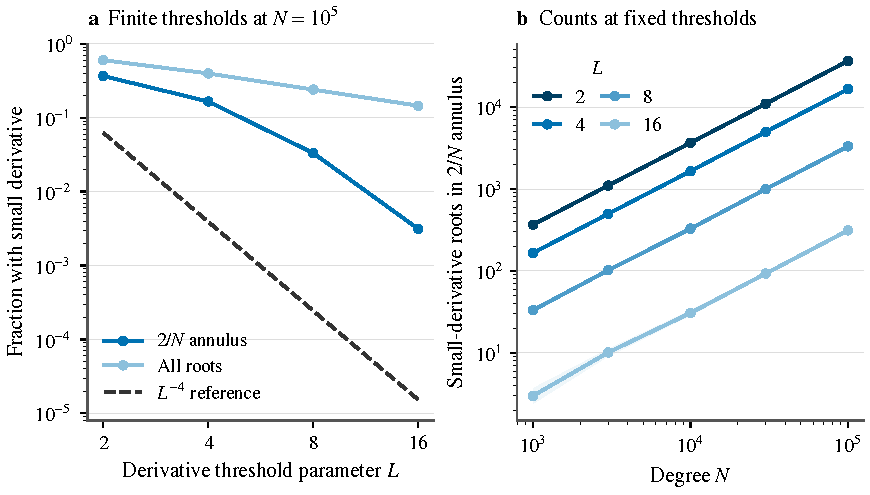
\includegraphics[width=\textwidth]{../numerics/publication/figures/small-derivative.pdf}
\caption{Zeros with small derivative, their fraction (a) and number (b)
over 77 sequences.}
\label{fig:small-derivative}
\end{figure}


\subsection{Bounds for appended tails}
\begin{lemma}[Appended tails]\label{lem:tails}
Let $K\ge2$, $N\ge\max\{4,K\}$ and $1\le m_{\max}\le N$. Set
\[
 \rho=1+K/N,\qquad g_m(z)=\sum_{k=N+1}^{N+m}\epsilon_kz^k,
 \qquad 0\le m\le m_{\max},
\]
and put
\[
 a=15e^{2K}\sqrt{m_{\max}\log N}.
\]
Outside an event of probability at most $N^{-10}$,
\[
 \max_{m\le m_{\max}}\sup_{|z|\le\rho}|g_m(z)|<a.
\]
\end{lemma}

\begin{proof}
As in the proof of Lemma~\ref{lem:second-derivative} for the second
derivative, we combine Hoeffding's inequality at the samples of the circle
$|z|=\rho$, a
deterministic bound on $g_m'$ between the samples, and the maximum
principle, now with the constants of the tails.

Note that the empty tail is identically zero.
We choose $\lceil N^3\rceil\le2N^3$ equally spaced samples on the boundary
circle. For every prefix, since $\rho\ge1$ and $k\le N+m\le2N$, we have
$\sum_{k=N+1}^{N+m}\rho^{2k}\le m\rho^{4N}\le m_{\max}e^{4K}$.
For a sample $z$ and $1\le m\le m_{\max}$, we apply Hoeffding's
inequality to
$\Re g_m(z)=\sum_{k=N+1}^{N+m}\epsilon_k\Re(z^k)$ and
$\Im g_m(z)=\sum_{k=N+1}^{N+m}\epsilon_k\Im(z^k)$, whose squared
coefficients are at most $|z|^{2k}=\rho^{2k}$. As in the proof of
Lemma~\ref{lem:second-derivative}, and since
$(2a/3)^2=100e^{4K}m_{\max}\log N$, we get
\begin{align*}
 \Prob\{|g_m(z)|\ge2a/3\}
 &\le\Prob\Bigl\{|\Re g_m(z)|\ge\frac{2a}{3\sqrt2}\Bigr\}
   +\Prob\Bigl\{|\Im g_m(z)|\ge\frac{2a}{3\sqrt2}\Bigr\}\\
 &\le4\exp\left[-\frac{(2a/3)^2}{4\sum_{k=N+1}^{N+m}\rho^{2k}}\right]
 \le4\exp\left[-\frac{(2a/3)^2}{4m_{\max}e^{4K}}\right]\\
 &=4\exp[-25\log N]=4N^{-25}.
\end{align*}
Since there are at most $2N^3$ samples and at most $m_{\max}\le N$
nonempty prefixes, there are at most $2N^4$ such pairs, and by the union
bound the probability that $|g_m(z)|\ge2a/3$ for one of them is at most
$(2N^4)(4N^{-25})=8N^{-21}\le N^{-10}$.
For the derivative we have the deterministic bound
\[
 \sup_{|z|\le\rho}|g_m'(z)|
 \le\sum_{k=N+1}^{N+m}k\rho^{k-1}
 \le m\cdot2N\cdot\rho^{2N}
 \le2Nm_{\max}e^{2K}.
\]
Since $N\ge K$, the circle $|z|=\rho$ has radius at most $2$ and length
at most $4\pi$, so that every
point of it lies within arc length $2\pi/N^3$ of a sample.
Therefore, since $m_{\max}\le\sqrt{m_{\max}}\sqrt N$ and
$4\pi<40\le5N^{3/2}\sqrt{\log N}$ for $N\ge4$, the error of
nearest-sample interpolation is at most
\[
 \frac{2\pi}{N^3}\cdot2Nm_{\max}e^{2K}
 =\frac{4\pi m_{\max}e^{2K}}{N^2}
 \le4\pi e^{2K}\sqrt{m_{\max}}\,N^{-3/2}
 <5e^{2K}\sqrt{m_{\max}\log N}
 =a/3.
\]
Outside this event, every point $\zeta$ of the circle of radius $\rho$ and
its nearest sample $z$ therefore satisfy, for $1\le m\le m_{\max}$,
\[
 |g_m(\zeta)|\le|g_m(z)|+\frac{4\pi m_{\max}e^{2K}}{N^2}
 <\frac{2a}3+\frac a3=a.
\]
By the maximum principle, the boundary bound extends to the disk.
Hence
$\max_{m\le m_{\max}}\sup_{|z|\le\rho}|g_m(z)|<a$
outside an event of probability at most $N^{-10}$, and this one event
controls every appended tail $g_m$ at once.
\end{proof}


\section{Root matching under perturbations}\label{sec:matching}

For a nonzero polynomial $P$, denote by $\nu_P(r)$ the number of roots of
$P$ in the closed disk $\{|z|\le r\}$, counted with multiplicity.

\begin{theorem}[Root matching]\label{thm:T4}
Let $P,Q=P+G$ be nonzero complex polynomials.
Let $D_1,\ldots,D_s$ be pairwise disjoint open disks, each containing
exactly one root of $P$ counted with multiplicity.  Suppose for a fixed
$a>0$ that
\[
 |P(z)|\geq a>|G(z)|\quad(z\in\partial D_j,\ 1\leq j\leq s).
\]
Denote by $c(r)$ the number of these disks whose closures meet $\{|z|=r\}$.
Then
\begin{equation}
 |\nu_Q(r)-\nu_P(r)|\leq c(r)+(\deg P-s)+\max(0,\deg Q-\deg P). \label{eq:T4}
\end{equation}
The same assertion holds for pairwise disjoint bounded open domains
whose boundaries are finite unions of smooth Jordan curves, with
exactly one root in each domain and the same boundary domination.
\end{theorem}

\begin{proof}
The idea is to find exactly one root of $Q$ in each selected domain by
Rouch\'e's theorem, and to count the other roots crudely, using the fact
that for each polynomial the number of them in $\{|z|\le r\}$ lies between
zero and their total number.

We use Rouch\'e's theorem in the form of
\cite[Chapter~4, Section~5.2, p.~153]{Ahlfors1979}. Let $\gamma$ be a
cycle that is homologous to zero in a region $\Omega$ and has winding
number $n(\gamma,z)\in\{0,1\}$ at every point $z$ off $\gamma$, and let
$f,g$ be analytic in $\Omega$ with $|f-g|<|f|$ on $\gamma$. Then $f$ and
$g$ have equally many zeros, counted with multiplicity, in
$\{z:n(\gamma,z)=1\}$.
We take $\Omega=\mathbb C$, in which every cycle is homologous to zero,
$f=P$, $g=Q$, and $\gamma=\partial D_j$, with its outer curve oriented
counterclockwise and its inner curves, if any, clockwise.
Since $D_j$ is the set of points inside its outer curve and outside its
inner curves, and a smooth Jordan curve winds once about each point
inside it and zero times about each point outside it, with the sign of its
orientation, we have $n(\partial D_j,z)=1$ for $z\in D_j$ and
$n(\partial D_j,z)=0$ for $z\notin\overline{D_j}$.
On $\partial D_j$ we have $|f-g|=|G|<a\le|P|=|f|$ by hypothesis.
Hence $D_j$ contains as many roots of $Q$ as of $P$, that is, exactly one,
counted with multiplicity.

Since the selected domains are pairwise disjoint and each of them contains
exactly one root of $P$ and exactly one root of $Q$, exactly $s$ roots of
each polynomial lie in these domains. We call the other roots unmatched.
Their numbers are $\deg P-s$ and $\deg Q-s=\deg P-s+\deg Q-\deg P$.
If the closure of a selected domain misses $\{|z|=r\}$, then, since the
domain is connected and the complement of the circle is the union of the
disjoint open sets $\{|z|<r\}$ and $\{|z|>r\}$, it lies entirely inside or
entirely outside that circle. Its root of $P$ is therefore counted by
$\nu_P(r)$ if and only if its root of $Q$ is counted by $\nu_Q(r)$, so
that this domain does not change the count.
On the other hand, each crossing domain, that is, one whose closure meets
the circle, changes the count by at most one, since each of its two roots
adds $0$ or $1$ to its count.
Hence the total change from selected roots is at most $c(r)$.

The numbers of unmatched roots inside the circle belong to
$[0,\deg P-s]$ and $[0,\deg Q-s]$, and their difference therefore has
absolute value at most
\[
 \max(\deg P-s,\deg Q-s)=\deg P-s+\max(0,\deg Q-\deg P),
\]
by the above expression for $\deg Q-s$.
Since $\nu_Q(r)-\nu_P(r)$ is the change from selected roots plus the
difference of the unmatched counts, we obtain \eqref{eq:T4} by the triangle
inequality.
Roots on the target circle are included in the inside count,
since the disk in $\nu_P(r)$ and $\nu_Q(r)$ is closed. Each selected root is
simple, since its total multiplicity is one.
\end{proof}

\begin{remark}\label{rem:T4-degree}
If $\deg Q\geq\deg P$, the last term in \eqref{eq:T4} is the degree difference.
For arbitrary degrees the positive part is necessary. Indeed, take
$P(z)=z^2$, $Q(z)=1$, no disks, and $0<r<1$. With the signed degree
difference we would have
\[
 2\nleq2+(0-2).
\]
\end{remark}
In this example we have $s=c(r)=0$, $\nu_P(r)=2$, since the double root $0$
lies in $\{|z|\le r\}$, and $\nu_Q(r)=0$, so that $|\nu_Q(r)-\nu_P(r)|=2$,
$\deg P-s=2$ and $\deg Q-\deg P=0-2$.

In the same way we can compare the root counts of $P$ and $Q$ in two
different disks.

\begin{corollary}[Matching across two radii]\label{cor:T4-two-radii}
Let $P$, $Q=P+G$ and the domains $D_1,\ldots,D_s$ satisfy the hypotheses of
Theorem~\ref{thm:T4}, in either of its forms. Let
$r,r'>0$, and denote by $c(r,r')$ the number of these domains whose
closures meet the closed annulus
$\{\min(r,r')\le|z|\le\max(r,r')\}$. Then
\[
 |\nu_Q(r')-\nu_P(r)|\leq c(r,r')+(\deg P-s)+\max(0,\deg Q-\deg P).
\]
\end{corollary}

\begin{proof}
Each domain $D_j$ contains exactly one root of $P$, by hypothesis, and
exactly one root of $Q$, by Rouch\'e's theorem on $\partial D_j$, applied
as in the proof of Theorem~\ref{thm:T4}, where $|G|<a\le|P|$. That step
does not involve the circle, so that only the counting changes. As
before, we call the remaining $\deg P-s$ roots of $P$ and $\deg Q-s$ roots
of $Q$ unmatched.
Let $A$ be the closed annulus between the two circles.
A domain $D_j$ whose closure misses $A$ lies in $\{|z|<\min(r,r')\}$ or in
$\{|z|>\max(r,r')\}$, since it is connected and the complement of $A$ is
the union of these two disjoint open sets. In the first case its root of
$P$ is counted by $\nu_P(r)$ and its root of $Q$ by $\nu_Q(r')$, and in
the second case neither is counted, so that the domain contributes the
same amount to $\nu_Q(r')$ and to $\nu_P(r)$. On the other hand, each of
the $c(r,r')$ remaining domains changes the difference by at most one,
since each of its two roots adds $0$ or $1$ to its count.
The numbers of unmatched roots counted by $\nu_P(r)$ and by $\nu_Q(r')$
belong to $[0,\deg P-s]$ and $[0,\deg Q-s]$, so that, as in the proof of
Theorem~\ref{thm:T4}, their difference has absolute value at most
$\deg P-s+\max(0,\deg Q-\deg P)$.
Since $\nu_Q(r')-\nu_P(r)$ is the sum of the two contributions, the
corollary follows from the triangle inequality by adding their bounds.
For $r=r'$ the annulus is the circle $\{|z|=r\}$, so that $c(r,r)=c(r)$,
and the bound reduces to \eqref{eq:T4}.
\end{proof}

\begin{lemma}[Disjoint sublevel domains near regular roots]
\label{lem:isolation-interface}
Let $a>0$ and let $\alpha$ be a root of a nonconstant polynomial $P$, with
$|P'(\alpha)|\geq d_0>0$.  Suppose
$|P''|\leq M_2$ throughout the closed disk of radius $2a/d_0$
around $\alpha$, and $4M_2a\leq d_0^2$.  Then
\[
 |P|\geq3a/2\quad\hbox{on }|z-\alpha|=2a/d_0,
\]
that disk contains exactly one root, and the component of
$\{|P|<a\}$ containing $\alpha$ lies inside it.
For any finite family of such roots with a common $a$, one can
choose a common level $b\in(a,3a/2)$ for which the corresponding
components of $\{|P|<b\}$ are pairwise disjoint bounded smooth
domains, each with exactly one root.  They satisfy the hypotheses of Theorem~\ref{thm:T4} whenever
$|G|<a$ on their closures.
\end{lemma}

\begin{proof}
The idea is to compare $P$ on the circle $|z-\alpha|=2a/d_0$ with its
linear part $P'(\alpha)(z-\alpha)$ at $\alpha$, using Taylor's theorem for
the lower bound on the circle and Rouch\'e's theorem for the single root
in the disk. For a family of roots we then choose a regular level $b$
between $a$ and $3a/2$, and the lower bound keeps each selected component
of $\{|P|<b\}$ inside the disk of its root.

Let $|z-\alpha|\le2a/d_0$. Then
\begin{align*}
 &|P(z)-P'(\alpha)(z-\alpha)|
 =|P(z)-P(\alpha)-P'(\alpha)(z-\alpha)|\\
 &\qquad=|z-\alpha|^2\Bigl|\int_0^1(1-u)P''(\alpha+u(z-\alpha))\dd u\Bigr|\\
 &\qquad\le M_2|z-\alpha|^2\int_0^1(1-u)\dd u
 =\frac{M_2}2|z-\alpha|^2,
\end{align*}
where the second equality is Taylor's theorem with integral remainder for
the function $u\mapsto P(\alpha+u(z-\alpha))$ on $[0,1]$, and the
inequality holds since $|P''|\le M_2$ on the segment from $\alpha$ to $z$,
which lies in the closed disk of radius $2a/d_0$ around $\alpha$.
For $|z-\alpha|=2a/d_0$, we therefore have
\begin{align*}
 |P(z)|&\geq|P'(\alpha)(z-\alpha)|-|P(z)-P'(\alpha)(z-\alpha)|
 \geq|P'(\alpha)||z-\alpha|-\frac{M_2}2|z-\alpha|^2\\
 &\geq d_0\cdot\frac{2a}{d_0}-\frac{M_2(2a/d_0)^2}2
 =2a-\frac{2M_2a^2}{d_0^2}
 \geq2a-\frac a2
 =\frac{3a}2,
\end{align*}
where the third inequality uses $|P'(\alpha)|\ge d_0$, and the last is the
hypothesis $4M_2a\le d_0^2$ multiplied by $a/(2d_0^2)$.

On the same circle, as in the chain above, we also have
\begin{align*}
 &|P(z)-P'(\alpha)(z-\alpha)|
 \le\frac{M_2}2|z-\alpha|^2
 =\frac{M_2(2a/d_0)^2}2
 =\frac{2M_2a^2}{d_0^2}
 \le\frac a2\\
 &\qquad<2a
 =d_0\cdot\frac{2a}{d_0}
 \le|P'(\alpha)||z-\alpha|
 =|P'(\alpha)(z-\alpha)|.
\end{align*}
Thus $f=P'(\alpha)(z-\alpha)$ and $g=P$ satisfy $|f-g|<|f|$ on the
circle. Rouch\'e's theorem, in the form used in the proof of
Theorem~\ref{thm:T4}, with $\Omega=\mathbb C$ and $\gamma$ the
counterclockwise circle, which winds once about each point of the open
disk and zero times about each point outside the closed disk, therefore
shows that $P$ has as many roots in the disk $|z-\alpha|<2a/d_0$ as the
linear polynomial $P'(\alpha)(z-\alpha)$, counted with multiplicity.
This linear polynomial is nonzero, since $|P'(\alpha)|\ge d_0>0$, and its
only root $\alpha$ lies in the disk.
Hence the open disk contains exactly one root,
and so does the closed disk, since $|P|\ge3a/2>0$ on the circle.
Since $|P|\ge3a/2>a$ on the boundary circle, the component of $\{|P|<a\}$
containing $\alpha$ does not meet this circle, and it therefore lies inside
the disk, since any connected set meeting both the interior and the
exterior of the disk meets its boundary.

For a finite family of roots, it suffices that the common level $b$
satisfies $b<3a/2$, so that the lower bound $|P|\ge3a/2$ on the circles
keeps the components inside the disks, and $b>a$, so that $|P|=b>a>|G|$ on
their boundaries. It must also avoid the values of $|P|$ at the zeros of
$P'$, so that the level $\{|P|=b\}$ is regular. We therefore choose
\[
 b\in(a,3a/2)\setminus\{|P(w)|:P'(w)=0\}.
\]
The excluded set is finite, since $P$ is nonconstant and $P'$ is a nonzero
polynomial with finitely many roots, and hence there exists such a $b$.
This level is regular, since by the Cauchy--Riemann equations the gradient
of $|P|^2$, written as a complex number, is $2P\overline{P'}$, and on
$\{|P|=b\}$ we have $P\ne0$ since $b>0$, and $P'\ne0$ by the choice of $b$.
The set $\{|P|=b\}$ is also compact, since it is closed, as $|P|$ is
continuous, and bounded, as $|P(z)|\to\infty$ as $|z|\to\infty$ for the
nonconstant polynomial $P$.
By the implicit function theorem, it is a compact smooth one-dimensional
manifold, and hence a finite union of smooth circles.

Let $\alpha$ be a designated root, that is, a
root of the family. Then the component of $\{|P|<b\}$ containing $\alpha$ is
connected and does not meet the circle $|z-\alpha|=2a/d_0$, where
$|P|\ge3a/2>b$, so that it lies inside this circle.
Since the disk contains exactly one root of $P$, the component contains
exactly its designated root. In particular, two designated roots lie in
distinct components, and distinct components of $\{|P|<b\}$ are disjoint.
Each component is open, as a component of an open set, and
bounded, since it lies in a disk. Its boundary lies in $\{|P|=b\}$, since
a boundary point $z$ satisfies $|P(z)|\le b$ by continuity, and if
$|P(z)|<b$, then a small disk about $z$ lies in $\{|P|<b\}$ and meets the
component, hence lies in it, which is impossible. Near each point of the
regular level $\{|P|=b\}$, the implicit function theorem shows that
$\{|P|<b\}$ is one side of the level curve. If the point lies on the
boundary of the component, then this side meets the component and, being
connected, lies in it, so that the nearby points of the curve lie on the
boundary as well. Consequently, the boundary of the component meets each of
the smooth circles above in an open and closed subset, and it is a union of
some of these circles.
These components are therefore disjoint bounded smooth domains, with
$|P|=b>a>|G|$ on their boundaries, by the choice of $b$ and the hypothesis
on $G$, and each of them contains exactly one root of $P$, counted with
multiplicity, so that they satisfy the hypotheses of Theorem~\ref{thm:T4}.
This holds even
when their localization disks overlap, since their disjointness comes from
the roots they contain, not from the disks.
\end{proof}

Figure~\ref{fig:phase-portrait} shows, for one polynomial with random
signs, the level curves of $|f_N|/\sigma_N(|z|)$ at the powers of $2$
around its zeros.

\begin{figure}[t]
\centering
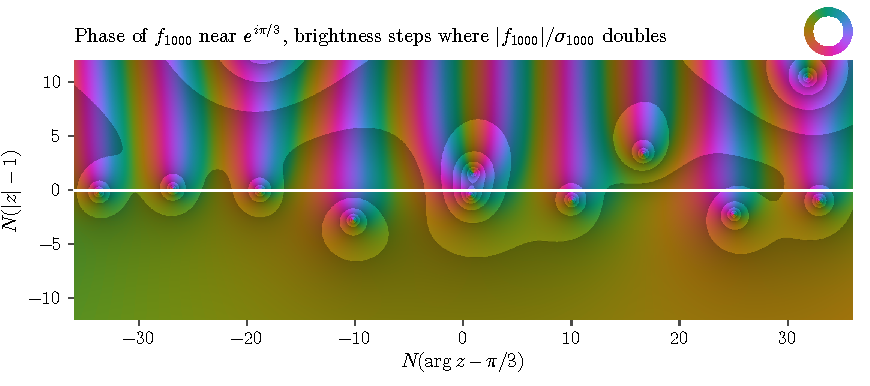
\includegraphics[width=0.85\textwidth]{figures/explanatory/phase-portrait.pdf}
\caption{Phase portrait of $f_{1000}$ near $e^{i\pi/3}$ for the sequence of
Figure~\ref{fig:root-matching}: the hue is $\arg f_{1000}$, all hues meet
at each zero, the brightness steps where $|f_{1000}|/\sigma_{1000}(|z|)$
doubles, and the white line is the unit circle. Near a zero with a large
derivative, $f_{1000}$ is nearly linear, so the small level curves are
nearly circles about it, like the boundaries of the disjoint disks about
the selected roots in Lemma~\ref{lem:isolation-interface}.}
\label{fig:phase-portrait}
\end{figure}


\section{Proof of the radial law}\label{sec:layer3}
In Section~\ref{sec:unit-circle} we first prove the unit-disk law,
Corollary~\ref{thm:stronglaw}. We then prove
Theorem~\ref{thm:radial-profile} in Section~\ref{sec:moving-radii}, by
the same construction at the moving radii $1+x/n$.

\subsection{The unit circle}\label{sec:unit-circle}
\begin{proof}[Proof of Corollary~\ref{thm:stronglaw}]
The idea is to compare every degree $n$ in a block
$j^8\le n\le(j+1)^8$ with the first degree $N=j^8$ of the block, by root
matching (Theorem~\ref{thm:T4}). A root of $f_N$ is matched unless it
lies outside the annulus $||z|-1|\le K/N$ or has a small derivative
there, and a matched root can cross the unit circle only if its domain
meets that circle.

\emph{Step 1: parameters.}
Fix an integer $K\ge2$. We compare the degrees
$N=j^8\le n\le(j+1)^8=N+m_j$.
In this proof the annulus is $||z|-1|\le K/N$, and, as in
Section~\ref{sec:derivative-detection}, $L=N^{1/64}$.
For the appended tails, let $\rho$ and $a$ be as in
Lemma~\ref{lem:tails}, with $K+2$ in place of $K$ and $m_{\max}=m_j$:
\[
 \rho=1+\frac{K+2}{N},\qquad
 a=15e^{2(K+2)}\sqrt{m_j\log N}.
\]
This lemma bounds every partial tail by $a$ on $|z|\le\rho$.
We write $M_2$ for the bound \eqref{eq:sign-second-derivative} of
Lemma~\ref{lem:second-derivative} on $|f_N''|$ over $|z|\le1+(K+1)/N$, and
$d_0$ for the derivative level of Lemma~\ref{lem:small-derivatives},
below which that lemma counts the annular roots in $B_{K,N}$:
\[
 M_2=100e^{K+4}N^{5/2}\sqrt{\log N},\qquad d_0=N^{3/2}/L.
\]
These parameters must satisfy the conditions of
Table~\ref{tab:unit-conditions}. All of them hold for $N$ beyond a
threshold that depends only on $K$, since the block exponent $8$ makes
$m_j$ of order $N^{7/8}$, and hence $a$ of order $N^{7/16}\sqrt{\log N}$,
while $d_0=N^{3/2-1/64}$.

\begin{table}[ht]
\centering
\small
\begin{tabular}{@{}l>{\raggedright\arraybackslash}p{0.46\textwidth}l@{}}
\toprule
Condition & Needed for & Holds by\\
\midrule
$m_j\le N$ & Lemma~\ref{lem:tails}
 & \eqref{eq:unit-block-length} and $N^{1/8}=j\ge9$\\
$N\ge K+2$ & Lemma~\ref{lem:tails} & large $j$\\
$2a/d_0\le1/N$ & Step~2: the disk of radius $2a/d_0$ about an annular
 root lies in $|z|\le1+(K+1)/N$, where $|f_N''|\le M_2$
 & \eqref{eq:unit-radius-scaled}\\
$4M_2a\le d_0^2$ & Step~2: the hypothesis of
 Lemma~\ref{lem:isolation-interface} & \eqref{eq:unit-parameters}\\
$2a/d_0<N^{-65/64}$ & Step~3: the half-width $N^{-65/64}$ of the thin
 band & \eqref{eq:unit-radius-ratio}\\
\bottomrule
\end{tabular}
\caption{The conditions on the parameters of Step~1 in
Section~\ref{sec:unit-circle}, which hold for all large $j$.}
\label{tab:unit-conditions}
\end{table}

With blocks $j^\beta$ in place of $j^8$, $m_j$ would be of order
$N^{1-1/\beta}$, and $2a/d_0$ and $4M_2a/d_0^2$ of orders
$N^{(1-1/\beta)/2-95/64}$ and $N^{(1-1/\beta)/2-15/32}$, up to
logarithmic factors, so that Steps~2 and~3 would need
$(1-1/\beta)/2<15/32$, that is, $\beta<16$. On the other hand, the bounds
of order $N^{-3/8}$ on the probabilities of the exceptional events in
Step~5 are summable along $N=j^\beta$ only if $3\beta/8>1$, that is,
$\beta>8/3$. The exponent $8$ lies in this range. More precisely, for
$j\ge60$, we have
\begin{align}
 m_j&=(j+1)^8-j^8\le8(j+1)^7=8\Bigl(1+\frac1j\Bigr)^7N^{7/8}\nonumber\\
 &\le8\Bigl(\frac{61}{60}\Bigr)^7N^{7/8}\le9N^{7/8},
 \label{eq:unit-block-length}\\
 a&\le45e^{2(K+2)}N^{7/16}\sqrt{\log N},\label{eq:unit-amplitude}\\
 \frac{2a}{d_0}
 &=\frac{2a}{N^{3/2-1/64}}
 \le90e^{2(K+2)}N^{7/16+1/64-3/2}\sqrt{\log N}\nonumber\\
 &=90e^{2(K+2)}N^{-67/64}\sqrt{\log N},\label{eq:unit-radius}\\
 \frac{2Na}{d_0}&\le90e^{2(K+2)}N^{-3/64}\sqrt{\log N}\longrightarrow0,
 \label{eq:unit-radius-scaled}\\
 \frac{4M_2a}{d_0^2}
 &=\frac{400e^{K+4}N^{5/2}\sqrt{\log N}\,a}{N^{3-1/32}}
 \le180\cdot100e^{K+4}\,e^{2(K+2)}N^{7/16+1/32-1/2}\log N\nonumber\\
 &=180\cdot100e^{K+4}\,e^{2(K+2)}N^{-1/32}\log N\longrightarrow0.
 \label{eq:unit-parameters}
\end{align}
In \eqref{eq:unit-block-length} we use the mean value theorem for the
eighth power on $[j,j+1]$, $j^7=N^{7/8}$, $j\ge60$ and $8(61/60)^7<9$,
and \eqref{eq:unit-amplitude} follows from it. In the last three bounds
we substitute \eqref{eq:unit-amplitude} and $d_0=N^{3/2-1/64}$.

\emph{Step 2: selected domains.}
We call an annular root $\alpha$, that is, a root of $f_N$ with
$||\alpha|-1|\le K/N$, good if $|f_N'(\alpha)|\ge N^{3/2}/L$.
If $|z-\alpha|\le2a/d_0$, then
$|z|\le|\alpha|+2a/d_0\le1+K/N+1/N=1+(K+1)/N<\rho$, since $2a/d_0\le1/N$
by Step~1.
Hence, outside the exceptional event of
Lemma~\ref{lem:second-derivative}, we have $|f_N''|\le M_2$ throughout
this disk, and Lemma~\ref{lem:isolation-interface}, applied with
$P=f_N$, $|f_N'(\alpha)|\ge d_0$ and $4M_2a\le d_0^2$, shows that the
disk contains exactly one zero and that $|f_N|\ge3a/2$ on its boundary.

Let $b\in(a,3a/2)$ be a common regular level.
By Lemma~\ref{lem:isolation-interface}, applied to the family of good
annular roots with the common amplitude $a$,
the selected components of $\{|f_N|<b\}$ are disjoint smooth bounded
domains. Each contains one zero and lies in its localization
disk, since it is connected, contains its root $\alpha$ and does not meet
the circle $|z-\alpha|=2a/d_0$, where $|f_N|\ge3a/2>b$.
The level may depend on $f_N$, but the estimates hold uniformly for every
regular level in this interval.
For a measurable choice, we take the first rational in $(a,3a/2)$,
in a fixed enumeration, outside the finite set of critical-value moduli.

\emph{Step 3: unselected roots and crossings.}
Let $U_N$ denote the number of unselected roots.
Since every good annular root selects a domain that contains no other
root, the unselected roots are the roots with $||\alpha|-1|>K/N$ and the
annular roots that are not good, which $B_{K,N}$ counts. Consequently,
\begin{align}
 U_N
 &\le\#\{\alpha:f_N(\alpha)=0,\ ||\alpha|-1|>K/N\}+B_{K,N},\nonumber\\
 \frac{U_N}{N}
 &\le\frac{2\log2}{K}+C(K)N^{-1/32}(\log N)^7+N^{-1/32}\nonumber\\
 &=\frac{2\log2}{K}+O_K\bigl(N^{-1/32}(\log N)^7\bigr),
 \label{eq:unit-unselected}
\end{align}
where the first count is bounded by \eqref{eq:sign-annular-mass} of
Corollary~\ref{cor:radial-probability}, and $B_{K,N}\le N^{31/32}$ by
Lemma~\ref{lem:small-derivatives}, outside the exceptional events of these
two results.
Let $c_N$ be the number of selected domains whose closures meet the unit
circle. The root of such a domain lies within $2a/d_0$ of the unit
circle, since the closure lies within $2a/d_0$ of the root and
$||\alpha|-1|\le|\alpha-z|$ for a point $z$ of the closure on the unit
circle. We count these roots with the thin-band bound
\eqref{eq:sign-thin-band} of Corollary~\ref{cor:radial-probability},
which controls $\nu_N$ at the radii $1+qN^{-1-\kappa}$ for
$0<\kappa\le1/64$. We take the largest value $\kappa=1/64$, so that the
two error terms $2N^{-\kappa}$ and $C(K)N^{\kappa-1/32}(\log N)^7$ of
\eqref{eq:sign-thin-band} are both $N^{-1/64}$, up to constants and the
factor $(\log N)^7$, and the band half-width $N^{-1-\kappa}=N^{-65/64}$ is
larger than $2a/d_0$ for large $N$, since $65/64<67/64$.
More precisely, by \eqref{eq:unit-radius} we have
\begin{equation}
 \begin{aligned}
 N^{65/64}\,\frac{2a}{d_0}
 &\le90e^{2(K+2)}N^{-67/64+1+1/64}\sqrt{\log N}\\
 &=90e^{2(K+2)}N^{-1/32}\sqrt{\log N}\longrightarrow0,
 \end{aligned}
 \label{eq:unit-radius-ratio}
\end{equation}
and, once $2a/d_0<N^{-65/64}$,
\begin{equation}
 \begin{aligned}
 c_N
 &\le\#\{\alpha:f_N(\alpha)=0,\ 1-N^{-65/64}<|\alpha|<1+N^{-65/64}\}\\
 &=\#\{\alpha:f_N(\alpha)=0,\ |\alpha|<1+N^{-65/64}\}-\nu_N(1-N^{-65/64})\\
 &\le\nu_N(1+N^{-65/64})-\nu_N(1-N^{-65/64}),
 \end{aligned}
 \label{eq:unit-crossings}
\end{equation}
where the first inequality holds since each such root satisfies
$||\alpha|-1|\le2a/d_0<N^{-65/64}$ and distinct domains have distinct
roots, and the equality since the inner inequality is strict.
We apply \eqref{eq:sign-thin-band} with $\kappa=1/64$ and with $2$ in
place of $K$, which suffices since the five radii $1+qN^{-65/64}$,
$q=-2,\dots,2$, lie within $2N^{-65/64}\le2/N$ of the unit circle. For all
sufficiently large $N$, outside five events, one at each of these radii,
we obtain
\begin{equation}
 \left|\frac{\nu_N(1+qN^{-65/64})}N-\frac12\right|
 \le2N^{-1/64}+C(2)N^{-1/64}(\log N)^7,
 \qquad q=-1,0,1.
 \label{eq:unit-thin-band}
\end{equation}
Dividing \eqref{eq:unit-crossings} by $N$ and centering at $\frac12$, we
obtain, whenever $2a/d_0<N^{-65/64}$,
\begin{equation}
 \begin{aligned}
 \frac{c_N}{N}
 &\le\frac{\nu_N(1+N^{-65/64})-\nu_N(1-N^{-65/64})}N\\
 &=\left(\frac{\nu_N(1+N^{-65/64})}N-\frac12\right)
      -\left(\frac{\nu_N(1-N^{-65/64})}N-\frac12\right)\\
 &\le\left|\frac{\nu_N(1+N^{-65/64})}N-\frac12\right|
      +\left|\frac{\nu_N(1-N^{-65/64})}N-\frac12\right|.
 \end{aligned}
 \label{eq:unit-crossings-centered}
\end{equation}
By the cases $q=\pm1$ of \eqref{eq:unit-thin-band}, it follows that
\[
 \frac{c_N}{N}\le4N^{-1/64}+2C(2)N^{-1/64}(\log N)^7
 =O\bigl(N^{-1/64}(\log N)^7\bigr)=o(1).
\]
By Theorem~\ref{thm:sign-logarithms}, each of the five events has
probability at most the right-hand side of
\eqref{eq:sign-log-concentration} at $K=2$, which is summable along
$N=j^8$, as noted after that theorem.
By the Borel--Cantelli lemma, almost surely only finitely many of these
events occur along $N=j^8$, and hence the case $q=0$ of
\eqref{eq:unit-thin-band} holds for all large $j$. Since its right-hand
side tends to zero, $\nu_N(1)/N\to1/2$ almost surely along $N=j^8$.

\emph{Step 4: comparison within a block.}
For $N<n\le N+m_j$, we write $f_n=f_N+g_{n-N}$, where $g_m$ is as in
Lemma~\ref{lem:tails}, with $K+2$ in place of $K$.
Since that lemma bounds all the partial tails at once, outside its tail
event we have $|g_{n-N}|<a$ on $|z|\le\rho$ simultaneously for all these
$n$, and $|z|\le\rho$ contains the closures of the selected domains by
Step~2.
By Lemma~\ref{lem:isolation-interface}, the selected domains then satisfy
the hypotheses of Theorem~\ref{thm:T4} with $P=f_N$, $G=g_{n-N}$ and
$Q=f_n$. Moreover, $\deg f_n=n$ and $\deg f_N=N$, since
$\epsilon_n,\epsilon_N\ne0$. Each of the $s$ selected domains contains
exactly one root of $f_N$, and the other roots of $f_N$ are the unselected
ones, so that $\deg f_N-s=N-s=U_N$.
By Theorem~\ref{thm:T4}, with degrees $N$ and $n$ and with $r=1$, where
$c(1)=c_N$, we have
\begin{align*}
 \max_{N<n\le N+m_j}|\nu_n(1)-\nu_N(1)|
 &\le\max_{N<n\le N+m_j}
      \bigl\{c_N+(\deg f_N-s)\\
 &\qquad+\max(0,\deg f_n-\deg f_N)\bigr\}\\
 &=\max_{N<n\le N+m_j}\bigl\{c_N+U_N+(n-N)\bigr\}=c_N+U_N+m_j.
\end{align*}
Since $m_j/N\to0$, the bound on $c_N/N$ in Step~3,
\eqref{eq:unit-unselected} and \eqref{eq:unit-block-length} give,
outside the exceptional events of Steps~1--4,
\begin{align*}
 \frac1N\max_{N<n\le N+m_j}|\nu_n(1)-\nu_N(1)|
 &\le\frac{c_N}N+\frac{U_N}N+\frac{m_j}N
 \le O\bigl(N^{-1/64}(\log N)^7\bigr)\\
 &\quad+\frac{2\log2}{K}+O_K\bigl(N^{-1/32}(\log N)^7\bigr)+9N^{-1/8}\\
 &=\frac{2\log2}{K}+o_K(1).
\end{align*}
For every degree $n$ in this block, the matching bound above, which holds
trivially for $n=N$, together with $N\le n$ and $n-N\le m_j$, yields
\begin{align}
 \left|\frac{\nu_n(1)}n-\frac12\right|
 &=\left|\frac Nn\left(\frac{\nu_N(1)}N-\frac12\right)
   +\frac{\nu_n(1)-\nu_N(1)}n-\frac{n-N}{2n}\right|\nonumber\\
 &\le \frac Nn\left|\frac{\nu_N(1)}N-\frac12\right|
       +\frac{c_N+U_N+m_j}{n}+\frac{n-N}{2n}\nonumber\\
 &\le \left|\frac{\nu_N(1)}N-\frac12\right|
       +\frac{c_N+U_N}{N}+\frac{3m_j}{2N}.
 \label{eq:unit-block}
\end{align}

\emph{Step 5: exceptional events, and $K\to\infty$.}
Let $E_{K,j}$ denote the common exceptional event in block $j$, the union
of the events of Table~\ref{tab:unit-events}, where $\Pi_K(N)$ is the
right-hand side of \eqref{eq:sign-log-concentration}. For all large $j$,
\begin{equation}
 \Prob(E_{K,j})
 \le4\Pi_K(N)+5\Pi_2(N)+N^{-3}+2N^{-10}+C(K)N^{-3/8}(\log N)^4.
                                                        \label{eq:unit-failure}
\end{equation}
In this bound the shared local-count and derivative events are counted
once each. We count the maximal-tail event once for the whole block,
since outside it the tail bound of Step~4 holds for all the degrees of
the block simultaneously.
With $N=j^8$ we have
$\Pi_K(j^8)=C(K)j^{-3}+j^{-96}+C(K)j^{-7/2}(8\log j)^{-12}$, since
$N^{-3/8}=j^{-3}$, $N^{-12}=j^{-96}$, $N^{-7/16}=j^{-7/2}$ and
$\log N=8\log j$, and \eqref{eq:unit-failure} reads
\[
 \Prob(E_{K,j})
 \le4\Pi_K(j^8)+5\Pi_2(j^8)+j^{-24}+2j^{-80}+C(K)j^{-3}(8\log j)^4.
\]
Hence, for each fixed $K$, every term of \eqref{eq:unit-failure} is
summable over $j$, since the exponents of $j$ are $-3$, $-96$, $-7/2$,
$-24$ and $-80$, and a power of $\log j$ does not affect the convergence.
In finite form, \eqref{eq:unit-failure} is \eqref{eq:block-failure}
with $R=2$, the width of the five thin-band events, and the root-count
bounds of Step~3 are \eqref{eq:block-unselected} and
\eqref{eq:block-center-crossings}.

\begin{table}[ht]
\centering
\small
\setlength{\tabcolsep}{4pt}
\begin{tabular}{@{}llll@{}}
\toprule
Event & Source & Used in & Probability\\
\midrule
Four radial events & \eqref{eq:sign-annular-mass}
 & Step~3, $U_N$ & $\Pi_K(N)$ each\\
Five thin-band events & \eqref{eq:sign-thin-band}, width $2$
 & Step~3, $c_N$, $\nu_N(1)$ & $\Pi_2(N)$ each\\
Local-count event & Lemma~\ref{lem:local-counts}
 & Step~3, $B_{K,N}$ & $N^{-3}$\\
Derivative event & Lemma~\ref{lem:second-derivative}
 & Steps~1--3 & $N^{-10}$\\
Mesh-deviation event & Lemma~\ref{lem:small-derivatives}
 & Step~3, $B_{K,N}$ & $C(K)N^{-3/8}(\log N)^4$\\
Maximal-tail event & Lemma~\ref{lem:tails} & Step~4 & $N^{-10}$\\
\bottomrule
\end{tabular}
\caption{The exceptional events whose union is $E_{K,j}$ in Step~5 of
Section~\ref{sec:unit-circle}. The derivative event is the event that
\eqref{eq:sign-second-derivative} fails, and the local-count, derivative
and mesh-deviation events are those of
Lemma~\ref{lem:small-derivatives}.}
\label{tab:unit-events}
\end{table}

Let $\Omega_K=(\limsup_j E_{K,j})^c$.
Since $\limsup_jE_{K,j}\subset\bigcup_{j\ge J}E_{K,j}$ for every $J$,
the summability above gives
$\Prob(\Omega_K^c)\le\lim_{J\to\infty}\sum_{j\ge J}\Prob(E_{K,j})=0$, and
since there are countably many integers $K\ge2$,
$\Prob(\bigcap_{K=2}^\infty\Omega_K)\ge1-\sum_{K=2}^\infty\Prob(\Omega_K^c)=1$.
On this intersection, for each $K\ge2$, all large $j$ and every $n$ with
$N\le n\le N+m_j$, the bounds \eqref{eq:unit-block}, the case $q=0$ of
\eqref{eq:unit-thin-band}, the bound on $c_N/N$ in Step~3,
\eqref{eq:unit-unselected} and \eqref{eq:unit-block-length} imply that
\begin{align*}
 \left|\frac{\nu_n(1)}n-\frac12\right|
 &\le\left|\frac{\nu_N(1)}N-\frac12\right|
      +\frac{c_N}N+\frac{U_N}N+\frac{3m_j}{2N}\\
 &\le2N^{-1/64}+C(2)N^{-1/64}(\log N)^7
      +4N^{-1/64}+2C(2)N^{-1/64}(\log N)^7\\
 &\quad+\frac{2\log2}{K}+C(K)N^{-1/32}(\log N)^7+N^{-1/32}
      +\frac{27}{2}N^{-1/8}.
\end{align*}
Since every large $n$ lies in such a block, and each term on the right
other than $2\log2/K$ tends to zero as $j\to\infty$, we conclude that
\[
 0\le\limsup_{n\to\infty}\left|\frac{\nu_n(1)}n-\frac12\right|
 \le\inf_{K\ge2}\frac{2\log2}{K}=0.
\]
\end{proof}

\begin{remark}[A deterministic block envelope]\label{rem:block-envelope}
There are deterministic numbers $\varepsilon_j\to0$ and events $E_j$,
defined on the original probability space, such that
$\sum_j\Prob(E_j)<\infty$ and, off $E_j$,
\[
 \max_{j^8\le n<(j+1)^8}\frac{|\nu_n(1)-\nu_{j^8}(1)|}{j^8}\le\varepsilon_j.
\]
\end{remark}

\begin{proof}
We apply Lemma~\ref{lem:deterministic-diagonalization} with the exponent
$8$, $n_j=j^8$ and $X_n=\nu_n(1)$, for which its conclusion is the
assertion of the remark. It requires, for each positive integer $k$,
numbers $a_k$, $b_k(j)$ and $p_k(j)$ such that, for every $j$,
\[
 \Prob\left\{\max_{n_j\le n<n_{j+1}}\frac{|X_n-X_{n_j}|}{n_j}
 >a_k+b_k(j)\right\}\le p_k(j),
\]
where $a_k\to0$ as $k\to\infty$, and where $b_k(j)\to0$ as $j\to\infty$
and $\sum_jp_k(j)<\infty$ for each fixed $k$.

Let $k$ be a positive integer, and put $K=k+1$, so that $K\ge2$, as the
proof of Corollary~\ref{thm:stronglaw} requires. Since every threshold in
that proof depends only on $K$, there is a deterministic $j_0(K)\ge60$
such that for every $j\ge j_0(K)$ the bound \eqref{eq:unit-failure} holds
and, outside the event $E_{K,j}$ of that proof, with $N=j^8$, the
matching bound of Step~4, \eqref{eq:unit-unselected}, the bound on
$c_N/N$ in Step~3 with $C(K)\ge4+2C(2)$, and
\eqref{eq:unit-block-length} give
\begin{align*}
 \max_{N<n\le N+m_j}|\nu_n(1)-\nu_N(1)|&\le c_N+U_N+m_j,\\
 \frac{U_N}N&\le\frac{2\log2}K+C(K)N^{-1/32}(\log N)^7+N^{-1/32},\\
 \frac{c_N}N&\le C(K)N^{-1/64}(\log N)^7,\\
 \frac{m_j}N&\le9N^{-1/8}.
\end{align*}
We set $a_k=2\log2/K$,
\[
 b_k(j)=C(K)N^{-1/32}(\log N)^7+N^{-1/32}
   +C(K)N^{-1/64}(\log N)^7+9N^{-1/8},
\]
and let $p_k(j)$ be the bound \eqref{eq:unit-failure} for
$\Prob(E_{K,j})$ when $j\ge j_0(K)$, and $p_k(j)=1$ when
$j<j_0(K)$.
Since the block $n_j\le n<n_{j+1}$ is contained in $N\le n\le N+m_j$,
and the increment vanishes at $n=N$, the four bounds above give, for
$j\ge j_0(K)$ and outside $E_{K,j}$,
\begin{align*}
 \max_{n_j\le n<n_{j+1}}\frac{|X_n-X_{n_j}|}{n_j}
 &\le\frac1N\max_{N<n\le N+m_j}|\nu_n(1)-\nu_N(1)|\\
 &\le\frac{c_N}N+\frac{U_N}N+\frac{m_j}N
 \le a_k+b_k(j).
\end{align*}
Hence the probability in the above requirement is at most
$\Prob(E_{K,j})\le p_k(j)$ when $j\ge j_0(K)$, and at most $1=p_k(j)$
when $j<j_0(K)$. Moreover, $a_k\to0$ as $k\to\infty$, and, for fixed
$k$, $b_k(j)\to0$ as $j\to\infty$ and $\sum_jp_k(j)<\infty$, since only
finitely many of its terms equal one and the others are summable by
Step~5 of that proof.
By Lemma~\ref{lem:deterministic-diagonalization}, there are therefore
deterministic $\varepsilon_j\to0$ and events $E_j$ with
$\sum_j\Prob(E_j)<\infty$, off which the normalized block increment is at
most $\varepsilon_j$. We may take $E_j$ to be the event on which the
normalized block increment exceeds $\varepsilon_j$, since it is contained
in the event given by the lemma. (In the proof of
Lemma~\ref{lem:deterministic-diagonalization} the given events are this
event for $j\ge J_1$ and $\Omega$ for $j<J_1$, where $J_1$ is the first of
the integers $J_k$ chosen there, and $\sum_{j\ge J_1}\Prob(E_j)\le1$.)
All the events here are defined through the random signs on
the original probability space.
\end{proof}

With $n_j=j^8$ and $X_n=\nu_n(1)$, the numbers $\varepsilon_j$ and the
events $E_j$ of Remark~\ref{rem:block-envelope} are those required by
Theorem~\ref{thm:T5}.

Figure~\ref{fig:root-matching} shows one block, from degree 1000 to
degree 1421, of the sequence with seed 522000.

\begin{figure}[t]
\centering
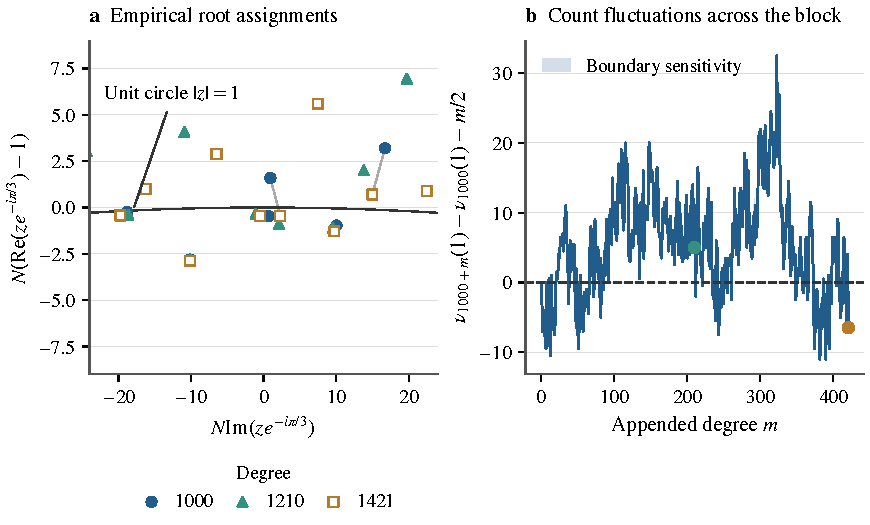
\includegraphics[width=\textwidth]{../numerics/publication/figures/root-matching.pdf}
\caption{Zeros of one sequence at degrees 1000, 1210 and 1421 near
$e^{i\pi/3}$, joined by an uncertified empirical assignment (a), and the
change in the count across the block (b).}
\label{fig:root-matching}
\end{figure}



\subsection{Moving radii}\label{sec:moving-radii}
\begin{proof}[Proof of Theorem~\ref{thm:radial-profile}]
The idea is to repeat the construction of Section~\ref{sec:unit-circle}
with the unit circle replaced by the circle of radius $1+x/N$, for one
$x$ at a time, comparing the degrees in a block by
Corollary~\ref{cor:T4-two-radii}, and then to pass to all $x$ by
monotonicity.

The profile in Proposition~\ref{prop:profiles} satisfies
\[
 F'=\Phi,\qquad 0\le\Phi\le1,\qquad
 0\le\Phi'=2\operatorname{Var}_x(t)\le\frac12.
\]
Here $F'=\Phi$ is part of Proposition~\ref{prop:profiles}, and
$0\le\Phi\le1$ since, by its definition in
Theorem~\ref{thm:radial-profile}, $\Phi(x)$ is the mean of $t$ under the
probability density proportional to $e^{2xt}$ on $[0,1]$. By
\eqref{eq:Phi-variance} in the proof of Lemma~\ref{lem:annular-mass},
$\Phi'(x)=2\operatorname{Var}_x(t)$, where $\operatorname{Var}_x(t)$ is
the variance of $t$ under the same density, and since the variance is at
most the mean square deviation from $\frac12$,
\[
 \operatorname{Var}_x(t)
 \le\frac{\int_0^1(t-\frac12)^2e^{2xt}\dd t}{\int_0^1e^{2xt}\dd t}
 \le\frac14.
\]

Fix $x$ and an integer $R\ge|x|+3$. We use the logarithmic bounds at the
radii $1+(x+qh)/N$, $|q|\le2$, for an offset $h\in(0,1]$ that must meet
the three requirements of Table~\ref{tab:moving-offset}, for the annular
width $K$ fixed below. The value $h=N^{-1/64}$ meets them, since the
quantities in the last column of that table tend to zero. For the first
degree $N=j^8$ of a block, we therefore set
\[
 h=N^{-1/64},\qquad r_N=1+x/N.
\]

\begin{table}[ht]
\centering
\small
\begin{tabular}{@{}>{\raggedright\arraybackslash}p{0.31\textwidth}
>{\raggedright\arraybackslash}p{0.43\textwidth}
>{\raggedright\arraybackslash}p{0.2\textwidth}@{}}
\toprule
Requirement & Reason & At $h=N^{-1/64}$\\
\midrule
$h\to0$ & the secants of $F$ over steps of length $h$ approximate
 $\Phi(x)$ with an error of order $h$ & $N^{-1/64}$\\[2pt]
$N^{-1/32}(\log N)^7/h\to0$ & the secants divide the logarithmic error
 $N^{-1/32}(\log N)^7$ of Theorem~\ref{thm:sign-logarithms} by $h$
 & $N^{-1/64}(\log N)^7$\\[2pt]
$h/N$ exceeds a bound of order $N^{-67/64}\sqrt{\log N}+N^{-9/8}$
 & the band of half-width $h/N$ about $|z|=1+x/N$ contains the root of
 every selected domain that meets the annulus between $|z|=1+x/N$ and
 $|z|=1+x/n$, for every degree $n$ of the block
 & $N^{-1/32}\sqrt{\log N}$ and $N^{-7/64}$\\
\bottomrule
\end{tabular}
\caption{The requirements on the offset $h$ in the proof of
Theorem~\ref{thm:radial-profile}, for fixed $K$ and $x$. The last column
gives $h$, the quotient in the first column, and the two terms of the
bound divided by $h/N$.}
\label{tab:moving-offset}
\end{table}

We apply Theorem~\ref{thm:sign-logarithms}, with $R$ in place of $K$, at
the five radii $r_q=1+y_q/N$, where $y_q=x+qh$ and $q=-2,-1,0,1,2$.
Since $h\le1$, we have $|y_q|\le|x|+2h<R$, so that every $r_q$ lies in
$[1-R/N,1+R/N]$. For all sufficiently large $N$, outside five exceptional
events, one at each radius $r_q$, this theorem gives
$|J_N(r_q)-\log\sigma_N(r_q)+\gamma/2|\le C(R)N^{-1/32}(\log N)^7$, and,
for $N\ge2R$, Lemma~\ref{lem:profile-rate} with $R$ in place of $K$ gives
$|\log\sigma_N(r_q)-\frac12\log N-F(y_q)|\le(R^2+e^{4R}/2)/N$. Adding the
two bounds, and using $1/N\le N^{-1/32}(\log N)^7$ for $N\ge3$, we get,
outside the five exceptional events,
\begin{align}
 \left|J_N(r_q)-\frac12\log N+\frac\gamma2-F(y_q)\right|
 &\le C(R)N^{-1/32}(\log N)^7+\frac{R^2+e^{4R}/2}N\nonumber\\
 &\le\eta_N:=(C(R)+R^2+e^{4R}/2)N^{-1/32}(\log N)^7.
 \label{eq:moving-probes}
\end{align}
For $q=-1,0,1$ we apply Lemma~\ref{lem:local-radial-secant} at $y_q$,
with $R$ in place of $K$, the centering $\frac12\log N$, the profile $F$
of Proposition~\ref{prop:profiles}, $M_F=1/2$ and $B_F=1$, which hold by
the bounds on $\Phi=F'$ above. Its logarithmic error is
$\eta_{\log}=C(R)N^{-1/32}(\log N)^7$, by
Theorem~\ref{thm:sign-logarithms} with $\E\log|G|=-\gamma/2$, and its
profile error is $\varepsilon=(R^2+e^{4R}/2)/N$, by
Lemma~\ref{lem:profile-rate} on $[-R,R]$ for $N\ge2R$, so that
$\eta_{\log}+\varepsilon\le\eta_N$ as in \eqref{eq:moving-probes}. The
lemma applies: outside the five exceptional events $J_N(r_q)$ is finite,
so that $f_N$ is nonzero; $|y_q|+h\le|x|+2h<R<N$, the last since
$N\ge2R$; and its three radii $1+(y_q-h)/N$, $r_q$ and $1+(y_q+h)/N$ are
among the five radii $r_{q'}$. Outside the five exceptional events it
gives
\[
 \left|\frac{\nu_N(r_q)}N-\Phi(y_q)\right|
 \le\frac h4+\frac RN+\frac{2\eta_N(1+R/N)}h.
\]
Since $|\Phi(y_q)-\Phi(x)|\le|q|h/2$ by $0\le\Phi'\le1/2$, since
$|q|h/2+h/4\le2h$ for $|q|\le1$ and $1+R/N\le2$, and since
$r_N+qh/N=r_q$, it follows that, for $q=-1,0,1$,
\begin{align}
 \left|\frac{\nu_N(r_N+qh/N)}N-\Phi(x)\right|
 &\le\frac{|q|h}{2}+\frac h4+\frac RN
       +\frac{2\eta_N(1+R/N)}h\nonumber\\
 &\le\varepsilon_N:=2h+\frac RN+\frac{4\eta_N}h\nonumber\\
 &=2N^{-1/64}+\frac RN+4(C(R)+R^2+e^{4R}/2)N^{-1/64}(\log N)^7\nonumber\\
 &=O_R\bigl(N^{-1/64}(\log N)^7\bigr).
 \label{eq:moving-secant}
\end{align}
Explicit constants for this estimate are given in \eqref{eq:E1-local}.
Moreover, the probabilities of the five logarithmic exceptional events
are summable along $N=j^8$, and $\varepsilon_N\to0$.
Subtracting the two endpoint counts and using \eqref{eq:moving-secant}
with $q=\pm1$, we get
\begin{align}
 &\#\{\alpha:f_N(\alpha)=0,\ ||\alpha|-r_N|<h/N\}\nonumber\\
 &\qquad=\#\{\alpha:f_N(\alpha)=0,\ |\alpha|<r_N+h/N\}-\nu_N(r_N-h/N)\nonumber\\
 &\qquad\le\nu_N(r_N+h/N)-\nu_N(r_N-h/N)\nonumber\\
 &\qquad=N\left(\frac{\nu_N(r_N+h/N)}N-\Phi(x)\right)
   +N\left(\Phi(x)-\frac{\nu_N(r_N-h/N)}N\right)\nonumber\\
 &\qquad\le2\varepsilon_NN,
 \label{eq:moving-band}
\end{align}
where the first equality holds since the inner inequality is strict.

Fix an integer annular width $K\ge R$, and let $a$, $\rho$, $d_0$, the
common regular level $b\in(a,3a/2)$ and the selected domains be those of
Steps~1 and~2 of Section~\ref{sec:unit-circle} at this width.
By Step~2, each selected domain contains exactly one root $\alpha$ of
$f_N$, and its closure lies in the closed disk of radius $2a/d_0$ about
$\alpha$, where $2a/d_0$ is bounded by \eqref{eq:unit-radius}.
For $N\le n\le N+m_j$, with $m_j=(j+1)^8-j^8$ as in Step~1 of
Section~\ref{sec:unit-circle}, the target radius moves by
$|(1+x/n)-(1+x/N)|=|x|(n-N)/(nN)\le|x|m_j/N^2$, and $m_j\le9N^{7/8}$ for
$j\ge60$ by \eqref{eq:unit-block-length}. Since $N/h=N^{65/64}$, these
bounds and \eqref{eq:unit-radius} yield
\begin{align*}
 \frac Nh\left(\frac{2a}{d_0}+\frac{|x|m_j}{N^2}\right)
 &\le90e^{2(K+2)}N^{-67/64+65/64}\sqrt{\log N}+9|x|N^{7/8-2+65/64}\\
 &=90e^{2(K+2)}N^{-1/32}\sqrt{\log N}+9|x|N^{-7/64}
 \longrightarrow0.
\end{align*}
Hence $2a/d_0+|x|m_j/N^2<h/N$ for all $N$ large enough, depending on $K$
and $x$.
Let $D$ be a selected domain whose closure meets the closed annulus
between the circles of radii $r_N$ and $1+x/n$, let $\alpha$ be its root
of $f_N$, and let $z$ be a point of this annulus in the closure of $D$.
Then $|z-\alpha|\le2a/d_0$, and $|z|$ lies between $r_N$ and $1+x/n$, so
that
\begin{align*}
 \bigl||\alpha|-r_N\bigr|
 &\le\bigl||\alpha|-|z|\bigr|+\bigl||z|-r_N\bigr|
 \le|\alpha-z|+\bigl||z|-r_N\bigr|\\
 &\le\frac{2a}{d_0}+\left|\left(1+\frac xn\right)-r_N\right|
 \le\frac{2a}{d_0}+\frac{|x|m_j}{N^2}<\frac hN.
\end{align*}
Hence the root of $f_N$ in such a domain lies in the strict band of
\eqref{eq:moving-band}. This is the case whenever two matched roots lie
on different sides of their respective target circles, since a connected
domain whose closure misses the closed annulus lies inside both circles
or outside both (proof of Corollary~\ref{cor:T4-two-radii}), the
complement of the closed annulus being the union of the disjoint open
sets inside the smaller circle and outside the larger one.
Since distinct domains have distinct roots, by \eqref{eq:moving-band}
the number $c(r_N,1+x/n)$ of these domains is at most $2\varepsilon_NN$.

As in Step~4 of Section~\ref{sec:unit-circle}, outside the tail event of
Lemma~\ref{lem:tails}, with $K+2$ in place of $K$ and $m_{\max}=m_j$, the
appended tail $f_n-f_N$ has modulus less than $a$ on $|z|\le\rho$, which
contains the selected domains, while $|f_N|>a$ on their boundaries. Since
this lemma bounds all the partial tails simultaneously, a single
maximal-tail event controls the entire block and all target radii.
The polynomials $f_N$ and $f_n$ have degrees exactly $N$ and $n$, since
their leading coefficients are $\pm1$, and, with $s$ the number of
selected domains and $U_N$ the number of unselected roots,
$\deg f_N-s=N-s=U_N$, as in Step~4. By
Corollary~\ref{cor:T4-two-radii}, with $P=f_N$, $Q=f_n$, $r=r_N$ and
$r'=1+x/n$, we have
\begin{align*}
 &\max_{N\le n\le N+m_j}|\nu_n(1+x/n)-\nu_N(r_N)|\\
 &\qquad\le\max_{N\le n\le N+m_j}\bigl\{c(r_N,1+x/n)+(\deg f_N-s)
   +\max(0,\deg f_n-\deg f_N)\bigr\}\\
 &\qquad=\max_{N\le n\le N+m_j}\bigl\{c(r_N,1+x/n)+U_N+(n-N)\bigr\}
 \le2\varepsilon_NN+U_N+m_j,
\end{align*}
and $U_N/N$ is bounded by \eqref{eq:unit-unselected} at this width $K$.

Let $E_{K,R,x,j}$ be the union of the events of
Table~\ref{tab:unit-events} at the width $K$, with the five thin-band
events replaced by the five logarithmic events of
Theorem~\ref{thm:sign-logarithms} at the width $R$ and the radii $r_q$.
With $\Pi_K(N)$ as in Step~5 of Section~\ref{sec:unit-circle}, and
$\Pi_R(N)$ the same with $R$ in place of $K$, for all large $j$,
\begin{equation}
 \Prob(E_{K,R,x,j})
 \le4\Pi_K(N)+5\Pi_R(N)+N^{-3}+2N^{-10}+C(K)N^{-3/8}(\log N)^4.
 \label{eq:moving-failure}
\end{equation}
This is \eqref{eq:unit-failure} with $5\Pi_2(N)$ replaced by
$5\Pi_R(N)$, and its finite form is \eqref{eq:block-failure}. At $N=j^8$
its terms are those of Step~5 of Section~\ref{sec:unit-circle} with
$\Pi_R$ in place of $\Pi_2$, so that, for each fixed $K,R,x$, it is
summable over $j$.

For $N\le n\le N+m_j$ we split $\nu_n(1+x/n)/n-\Phi(x)$ into three
terms, and by \eqref{eq:moving-secant} with $q=0$, the matching bound
above, $N\le n\le N+m_j$ and $0\le\Phi\le1$, we have
\begin{align*}
 \left|\frac{\nu_n(1+x/n)}n-\Phi(x)\right|
 &=\biggl|\frac Nn\left(\frac{\nu_N(r_N)}N-\Phi(x)\right)\\
 &\qquad+\frac{\nu_n(1+x/n)-\nu_N(r_N)}n-\frac{n-N}n\Phi(x)\biggr|\\
 &\le \frac Nn\left|\frac{\nu_N(r_N)}N-\Phi(x)\right|
 +\frac{|\nu_n(1+x/n)-\nu_N(r_N)|}{n}\\
 &\quad+\frac{n-N}{n}\Phi(x)
 \le\varepsilon_N+\frac{2\varepsilon_NN+U_N+m_j}N+\frac{m_j}N\\
 &= 3\varepsilon_N+\frac{U_N}N+\frac{2m_j}N.
\end{align*}

Let $\Omega_{K,R,x}=(\limsup_jE_{K,R,x,j})^c$. As in Step~5 of
Section~\ref{sec:unit-circle}, the summability of
\eqref{eq:moving-failure} gives
$\Prob(\Omega_{K,R,x}^c)\le\lim_{J\to\infty}\sum_{j\ge J}\Prob(E_{K,R,x,j})=0$.
On $\Omega_{K,R,x}$ the preceding bounds hold for all large $j$, and
hence, by \eqref{eq:unit-unselected} and $m_j\le9N^{7/8}$, for all large
$j$ and $N\le n\le N+m_j$ we get
\[
 \left|\frac{\nu_n(1+x/n)}n-\Phi(x)\right|
 \le3\varepsilon_N+\frac{2\log2}K+C(K)N^{-1/32}(\log N)^7
 +N^{-1/32}+18N^{-1/8}.
\]
Every large $n$ lies in such a block, and each term on the right other
than $2\log2/K$ tends to zero as $j\to\infty$.
Hence, on the intersection $\Omega_x$ of the events $\Omega_{K,R,x}$ over
integers $K\ge R$, which has probability one as a countable intersection
of events of probability one,
\[
 0\le\limsup_{n\to\infty}
       \left|\frac{\nu_n(1+x/n)}n-\Phi(x)\right|
 \le\frac{2\log2}{K}\longrightarrow0
 \qquad(K\to\infty).
\]
As a countable intersection, the rational event
$\bigcap_{x\in\mathbb Q}\Omega_x$ also has probability one.

For any real $x$, choose rationals $x_-<x<x_+$. By monotonicity we have
$\nu_n(1+x_-/n)/n\le\nu_n(1+x/n)/n\le\nu_n(1+x_+/n)/n$, and taking
limits on the rational event we get
\[
 \Phi(x_-)\le\liminf_{n\to\infty}\frac{\nu_n(1+x/n)}n
 \le\limsup_{n\to\infty}\frac{\nu_n(1+x/n)}n
 \le\Phi(x_+).
\]
Letting $x_-$ increase to $x$ and $x_+$ decrease to $x$ through
rationals, the continuity of $\Phi$ shows that the limit inferior and the
limit superior are both $\Phi(x)$.
To prove the uniform convergence, fix a compact interval $I$ and
$\delta>0$, write $\widehat\Phi_n(x)=\nu_n(1+x/n)/n$, and choose rational
numbers $x_0<x_1<\cdots<x_M$ with $I\subset(x_0,x_M)$ and
$x_{i+1}-x_i<\delta$. For $x\in[x_i,x_{i+1}]\cap I$ we have
\[
 \widehat\Phi_n(x_i)-\Phi(x_{i+1})
 \le\widehat\Phi_n(x)-\Phi(x)
 \le\widehat\Phi_n(x_{i+1})-\Phi(x_i),
\]
since $\widehat\Phi_n$ is nondecreasing, as $\nu_n$ is, and $\Phi$ is
nondecreasing, as $\Phi'\ge0$.
Taking the supremum over $x\in I$, we get
\begin{align*}
 \sup_{x\in I}|\widehat\Phi_n(x)-\Phi(x)|
 &\le \max_{0\le i\le M}|\widehat\Phi_n(x_i)-\Phi(x_i)|
       +\max_{0\le i<M}\{\Phi(x_{i+1})-\Phi(x_i)\}\\
 &\le \max_{0\le i\le M}|\widehat\Phi_n(x_i)-\Phi(x_i)|
       +\frac{\delta}{2},
\end{align*}
where the second inequality follows from $|\Phi'|\le1/2$ and
$x_{i+1}-x_i<\delta$ by the mean value theorem.
On the rational event the maximum tends to zero, and we then let
$\delta$ tend to zero.
Finally, we intersect over intervals with integer endpoints.
All these intersections take place on the given probability space.
Since the rational event does not depend on $I$, the uniform convergence
holds on it for every compact interval $I$ at once, and in particular for
$I=[-A,A]$ for every $A>0$, which is the assertion of
Theorem~\ref{thm:radial-profile}.
\end{proof}

\section{Other coefficient distributions}
\label{sec:layer2-models}\label{par:central-symmetry}
We now take one sequence of iid coefficients with one of the
distributions below, use the same sequence at every degree, and write
\[
 f_N(z)=\sum_{k=0}^N\xi_kz^k,\qquad
 \sigma_N(r)^2=\mathbb E|\xi_0|^2\sum_{k=0}^Nr^{2k},
\]
and, as in Section~\ref{sec:concentration},
$X_r(\theta)=f_N(re^{i\theta})/\sigma_N(r)$.
In the three classes for which we prove a root law, the coefficients have
mean zero and positive second moment.
We define the logarithmic integral $J_N$ and the closed-disk zero count
as before.

We first bound the local zero counts.
Steinhaus and bounded centrally symmetric coefficients have the law
of independent signs times bounded amplitudes, so that
Lemma~\ref{lem:local-counts-general} applies to them, while
Gaussian amplitudes are unbounded, and we treat them separately in
Lemma~\ref{lem:local-counts-gauss}.

\begin{lemma}[Local zero counts for Steinhaus coefficients]
\label{lem:local-counts-steinhaus}
Let the $\xi_k$ be independent and uniform on the unit circle.
Fix $K\ge2$, and put
\[
 A=\max(1,1024\pi/c_{\rm HW}),\qquad t_N=\frac{A\log N}{N},\qquad
 C_1(K)=\frac{4A+4K+4}{\log2}.
\]
Let $N\ge e$ with $t_N\le1$.
Except on an event of probability at most $N^{-3}$, every disk
\[
 \{z:|z-z_0|\le2K/N\},\qquad ||z_0|-1|\le1/N,
\]
contains at most $C_1(K)\log N$ zeros of $f_N$.
\end{lemma}

\begin{proof}
The idea is to write each coefficient as a sign times a point of a fixed
semicircle and to apply Lemma~\ref{lem:local-counts-general}.
The event in the lemma depends only on the law of
$(\xi_0,\dots,\xi_N)$.
Let the $Z_k$ be uniform on a fixed semicircle, independent of each other
and of the signs.
Since $-e^{i\varphi}=e^{i(\varphi+\pi)}$, the products $\epsilon_kZ_k$
are independent and uniform on the unit circle, so we may take
$\xi_k=\epsilon_kZ_k$.
Since $|Z_k|=1$ and $\sum_{k=0}^N|Z_k|^2=N+1$, we may apply
Lemma~\ref{lem:local-counts-general} with $a_k=Z_k$, $B=1$,
$\eta=1$ and $\mathcal E=\Omega$.
Then $P_N=f_N$, and, since $\log1=0$, the constants of that lemma are
\begin{align*}
 A(1,1)&=\max(1,1024\pi/c_{\rm HW})=A,\qquad t_N(1,1)=t_N,\\
 C_1(K,1,1)&=\frac{4A+4K+4}{\log2}=C_1(K).
\end{align*}
This proves the lemma.
\end{proof}

\begin{lemma}[Local zero counts for bounded coefficients]
\label{lem:local-counts-bounded}
Let the $\xi_k$ be independent with a fixed nondegenerate distribution on
$\mathbb R$ or $\mathbb C$ that is centrally symmetric, that is,
$\operatorname{Law}(\xi_0)=\operatorname{Law}(-\xi_0)$, and normalize
\[
 \mathbb E|\xi_0|^2=1,\qquad |\xi_0|\le B,\qquad B\ge1.
\]
Fix $K\ge2$, and put
\[
 A_B=\max(1,2048\pi B^2/c_{\rm HW}),\qquad
 t_{N,B}=\frac{A_B\log N}{N},
\]
\[
 C_{1,B}(K)=\frac{4A_B+4K+4+\log B}{\log2}.
\]
Let $N\ge e$ with $t_{N,B}\le1$.
Except on an event of probability at most
$\exp[-(N+1)/(2B^4)]+N^{-3}$, every disk
\[
 \{z:|z-z_0|\le2K/N\},\qquad ||z_0|-1|\le1/N,
\]
contains at most $C_{1,B}(K)\log N$ zeros of $f_N$.
\end{lemma}

\begin{proof}
The idea is to write each coefficient as a sign times an independent copy
of itself, to bound the probability that the amplitudes have small total
energy, and to apply Lemma~\ref{lem:local-counts-general} with
$\eta=\tfrac12$.
The event in the lemma depends only on the law of
$(\xi_0,\dots,\xi_N)$.
Let $a_0,\dots,a_N$ be independent with the coefficient distribution, and
independent of the signs.
By symmetry,
$\operatorname{Law}(\epsilon_ka_k)
 =\tfrac12\operatorname{Law}(a_k)+\tfrac12\operatorname{Law}(-a_k)
 =\operatorname{Law}(\xi_k)$,
and the products are independent, so that we may take
$\xi_k=\epsilon_ka_k$.
Let $\mathcal E=\{\sum_{k=0}^N|a_k|^2\ge(N+1)/2\}$.
Since $|a_k|^2\in[0,B^2]$ and $\mathbb E|a_k|^2=1$, it follows from
Hoeffding's inequality \cite[Theorem~2]{Hoeffding1963} for the $N+1$
variables $|a_k|^2$ at the deviation $(N+1)/2$ that
\begin{align*}
 \Prob(\mathcal E^c)
 &=\Prob\left\{\sum_{k=0}^N(|a_k|^2-1)<-\frac{N+1}2\right\}\\
 &\le\exp\left[-\frac{2((N+1)/2)^2}{(N+1)B^4}\right]
 =\exp\left[-\frac{N+1}{2B^4}\right].
\end{align*}
We apply Lemma~\ref{lem:local-counts-general} with these $a_k$, this
$B$, $\eta=\tfrac12$ and this event $\mathcal E$.
Then $P_N=f_N$, and the constants of that lemma are
\begin{align*}
 A(B,\tfrac12)&=\max\left(1,\frac{1024\pi B^2}{c_{\rm HW}/2}\right)
 =\max\left(1,\frac{2048\pi B^2}{c_{\rm HW}}\right)=A_B,\\
 t_N(B,\tfrac12)&=\frac{A_B\log N}N=t_{N,B},\\
 C_1(K,B,\tfrac12)&=\frac{4A_B+4K+4+\log B}{\log2}=C_{1,B}(K).
\end{align*}
It follows that the probability that $\mathcal E$ occurs and some disk
contains more than $C_{1,B}(K)\log N$ zeros is at most $N^{-3}$.
Adding $\Prob(\mathcal E^c)$ proves the lemma.
\end{proof}

\begin{lemma}[Local zero counts for Gaussian coefficients]
\label{lem:local-counts-gauss}
Let $\xi_k=g_k$, where the $g_k$ are independent standard real
Gaussians, or let $\xi_k=(g_k+ih_k)/\sqrt2$, where all $g_k,h_k$ are
independent standard real Gaussians.
Fix $K\ge2$, let $t_N$ and $C_1(K)$ be as in
Lemma~\ref{lem:local-counts-steinhaus}, and put
\[
 C_{1,G}(K)=C_1(K)+\frac2{\log2}.
\]
Let $N\ge e$ with $t_N\le1$.
Except on an event of probability at most $N^{-3}+e^{-3(N+1)/32}$,
every disk
\[
 \{z:|z-z_0|\le2K/N\},\qquad ||z_0|-1|\le1/N,
\]
contains at most $C_{1,G}(K)\log N$ zeros of $f_N$.
\end{lemma}

\begin{proof}
Since the Gaussian amplitudes are unbounded,
Lemma~\ref{lem:local-counts-general} does not apply, but its proof still
works once $|f_N|$ is bounded outside an event of exponentially small
probability.
Let $J$, the arcs $I$ and the real Gram matrix $A_I$ be those of the
proof of Lemma~\ref{lem:local-counts-general} with $a_k=1$, $B=1$ and
$\eta=1$, so that $J\le8N$,
$\mu(I)=t_N/\pi$, the eigenvalues of $A_I$ lie in $[0,1]$,
$\operatorname{tr}A_I=(N+1)t_N/\pi$, $\|A_I\|\le1$ and
$\|A_I\|_{\rm HS}^2\le\operatorname{tr}A_I$.
Let $Q_I=\int_I|f_N(e^{i\theta})|^2\dd\mu(\theta)$.

\emph{Real coefficients.}
With $g=(g_0,\dots,g_N)$, we have $Q_I=g^TA_Ig$ and
$\mathbb EQ_I=\operatorname{tr}A_I$, since
$\mathbb Eg_jg_k=\mathbf 1\{j=k\}$.
Standard real Gaussian coordinates have $\psi_2$ norm at most two in the
moment convention of Section~\ref{sec:local-root-count}.
Indeed, $y^{p/2}e^{-y/4}\le(2p/e)^{p/2}$ for $y\ge0$, and
$\mathbb Ee^{g_k^2/4}=(1-\tfrac12)^{-1/2}=\sqrt2$, so that, writing
$|g_k|^p=(g_k^2)^{p/2}e^{-g_k^2/4}\cdot e^{g_k^2/4}$, for $p\ge1$ we have
\[
 p^{-1/2}(\mathbb E|g_k|^p)^{1/p}
 \le p^{-1/2}\bigl(\sqrt2\,(2p/e)^{p/2}\bigr)^{1/p}
 =2^{1/(2p)}(2/e)^{1/2}
 \le2/\sqrt e<2.
\]
Therefore \eqref{eq:HW-signs} holds with $g$ in place of $\epsilon$, and
the Hanson--Wright chain in the proof of
Lemma~\ref{lem:local-counts-general} at $B=\eta=1$ gives
$\Prob\{Q_I<\tfrac12\operatorname{tr}A_I\}\le2N^{-16}$.

\emph{Complex coefficients.}
For an arc $I$, the complex Gram matrix is given by
\[
 M_{jk}=\int_Ie^{i(k-j)\theta}\dd\mu(\theta),\qquad 0\le j,k\le N,
\]
so that, expanding the square,
\[
 Q_I=\int_I\left|\sum_{k=0}^N\xi_ke^{ik\theta}\right|^2\dd\mu(\theta)
 =\sum_{j,k}\overline{\xi_j}M_{jk}\xi_k.
\]
For a complex vector $x$, the same expansion and Parseval's identity show
that
$\sum_{j,k}\overline{x_j}M_{jk}x_k=\int_I|\sum_kx_ke^{ik\theta}|^2\dd\mu$
lies between $0$ and $\int|\sum_kx_ke^{ik\theta}|^2\dd\mu=\|x\|^2$, so
that the eigenvalues of $M$ lie in $[0,1]$, and
$\operatorname{tr}M=(N+1)\mu(I)$.
We write the arc energy as a quadratic form in the real vector
$(g,h)=(g_0,\ldots,g_N,h_0,\ldots,h_N)$ with the matrix
\[
 \widetilde M=\frac12
 \begin{pmatrix}\Re M&-\Im M\\\Im M&\Re M\end{pmatrix}.
\]
Indeed, since
$\xi_k=(g_k+ih_k)/\sqrt2$, $Q_I$ is real and $M=\Re M+i\Im M$, taking real
parts in $Q_I=\tfrac12(g-ih)^TM(g+ih)$ we get
\[
 Q_I=\tfrac12\bigl\{g^T(\Re M)g+h^T(\Re M)h+h^T(\Im M)g-g^T(\Im M)h\bigr\}
 =(g,h)^T\widetilde M(g,h).
\]
Let $\lambda_\ell$ be the eigenvalues of $M$.
If $Mv=\lambda_\ell v$, then taking real and imaginary parts shows that
$(\Re v,\Im v)$ and $(-\Im v,\Re v)$ are eigenvectors of $\widetilde M$
with eigenvalue $\lambda_\ell/2$, and for an orthonormal eigenbasis of $M$
these $2N+2$ real vectors are orthonormal.
Hence each $\lambda_\ell/2$ occurs twice as an eigenvalue of
$\widetilde M$, so that, since $\lambda_\ell^2\le\lambda_\ell$ for
$\lambda_\ell\in[0,1]$, we have
$\widetilde M\ge0$, $\operatorname{tr}\widetilde M=\operatorname{tr}M$,
$\|\widetilde M\|\le\frac12$ and
$\|\widetilde M\|_{\rm HS}^2
 =\frac12\sum_\ell\lambda_\ell^2\le\operatorname{tr}M/2$.
In particular $\mathbb EQ_I=\operatorname{tr}\widetilde M=\operatorname{tr}M$,
since the $2N+2$ coordinates of $(g,h)$ are independent standard Gaussians.
As in the real case, the $g_k$ and $h_k$ have moment $\psi_2$ norm at
most two, so that the Hanson--Wright inequality at deviation
$\operatorname{tr}M/2$ and the bounds on $\|\widetilde M\|_{\rm HS}^2$
and $\|\widetilde M\|$ give, for each arc,
\begin{align*}
 \Prob\{Q_I<\operatorname{tr}M/2\}
 &\le2\exp\left[-c_{\rm HW}\min\left\{
   \frac{(\operatorname{tr}M/2)^2}{16\|\widetilde M\|_{\rm HS}^2},
   \frac{\operatorname{tr}M/2}{4\|\widetilde M\|}\right\}\right]\\
 &\le2\exp[-c_{\rm HW}\min\{\operatorname{tr}M/32,\operatorname{tr}M/4\}]
 =2e^{-c_{\rm HW}\operatorname{tr}M/32}\\
 &\le2e^{-c_{\rm HW}\operatorname{tr}M/64}
 =2\exp\left[-\frac{c_{\rm HW}(N+1)t_N}{64\pi}\right]
 \le2N^{-16},
\end{align*}
since $\operatorname{tr}M=(N+1)\mu(I)=(N+1)t_N/\pi$, as in the real case.

\emph{Both cases.}
In both cases $\mathbb EQ_I=(N+1)\mu(I)$, and, by the union bound over at
most $8N$ arcs,
$\Prob\{Q_I<\tfrac12\mathbb EQ_I\text{ for some arc }I\}
 \le(8N)(2N^{-16})=16N^{-15}\le N^{-3}$.
On the complement of this event, averaging over each closed arc gives
$\max_{\theta\in I}|f_N(e^{i\theta})|^2\ge Q_I/\mu(I)\ge(N+1)/2$,
and by continuity there exists $z_1=e^{i\theta_1}$ on the arc such that
$|f_N(z_1)|^2\ge(N+1)/2$.
Given $z_0$, we take such a $z_1$ on the arc of the angular center
nearest to $z_0/|z_0|$. As in the proof of
Lemma~\ref{lem:local-counts-general}, the target disk then lies strictly
within $\{|z-z_1|<R\}$, where $R=(2K+1)/N+2t_N$.

For the energy, let $S=\sum_{k=0}^N|\xi_k|^2$, which is
$\sum_{k=0}^Ng_k^2$ in the real case.
For $0\le y\le1/8$ and real coefficients $\xi_k=g_k$, we have
$\mathbb Ee^{yg_k^2}=(1-2y)^{-1/2}$, and hence
\[
 \log\mathbb Ee^{y(g_k^2-1)}
 =-y-\tfrac12\log(1-2y)
 =\sum_{j\ge2}\frac{2^{j-1}y^j}{j}
 \le\frac{y^2}{1-2y}\le2y^2,
\]
since $2^{j-1}/j\le2^{j-2}$ for $j\ge2$,
$\sum_{j\ge2}2^{j-2}y^j=y^2/(1-2y)$ and $1-2y\ge3/4$.
For complex coefficients, $|\xi_k|^2$ has the exponential distribution
with mean one, so that $\mathbb Ee^{y|\xi_k|^2}=(1-y)^{-1}$ and
\[
 \log\mathbb Ee^{y(|\xi_k|^2-1)}
 =-y-\log(1-y)
 =\sum_{j\ge2}\frac{y^j}{j}
 \le\frac{y^2}{2(1-y)}\le2y^2,
\]
since $1/j\le1/2$ for $j\ge2$ and $1-y\ge7/8$.
In both cases, by independence, the exponential Markov inequality at
$y=1/8$ and the bound $2y^2=2/64$ for each of the $N+1$ factors, we have
\begin{align*}
 \Prob\left\{\sum_{k=0}^N|\xi_k|^2>2(N+1)\right\}
 &\le e^{-2(N+1)/8}\,\mathbb Ee^{S/8}
 =e^{-(N+1)/8}\,\mathbb Ee^{(S-(N+1))/8}\\
 &=e^{-(N+1)/8}\prod_{k=0}^N\mathbb Ee^{(|\xi_k|^2-1)/8}\\
 &\le\exp\left[-\frac{N+1}8+\frac{2(N+1)}{64}\right]
 =e^{-3(N+1)/32}.
\end{align*}
On the complement of this event, the Cauchy--Schwarz inequality bounds the
polynomial in the local Jensen disk by
\begin{align*}
 |f_N(z)|&\le\left(\sum_{k=0}^N|\xi_k|^2\right)^{1/2}
 \left(\sum_{k=0}^N|z|^{2k}\right)^{1/2}\\
 &\le\sqrt{2(N+1)}\sqrt{N+1}\,e^{2NR}
 =\sqrt2(N+1)e^{2NR},
\end{align*}
for $|z-z_1|\le2R$, where $|z|\le1+2R\le e^{2R}$, so that
$\sum_{k=0}^N|z|^{2k}\le(N+1)e^{4NR}$.
By the zero-count step \cite[\S8.21]{Titchmarsh1939} and Jensen's formula
\cite[\S3.61]{Titchmarsh1939} at the nonzero center value, as in the
proof of Lemma~\ref{lem:local-counts-general}, and by the two bounds on
$|f_N|$ above, we have
\begin{align*}
 \#\{\alpha:|\alpha-z_1|<R\}
 &\le\frac{\log\bigl(\sqrt2(N+1)e^{2NR}\bigr)
   -\tfrac12\log\bigl((N+1)/2\bigr)}{\log2}\\
 &\le C_1(K)\log N+\frac12
 \le C_{1,G}(K)\log N.
\end{align*}
The middle step is the last display of that proof at $B=\eta=1$, whose
maximum bound $(N+1)e^{2NR}$ lacks the factor $\sqrt2$, which adds
$\log\sqrt2/\log2=\tfrac12$, and the last step holds since
$\tfrac12\le(2/\log2)\log N$ for $N\ge2$.
\end{proof}

In the radial estimates below, $K\ge2$ is fixed, $N$ is sufficiently
large, and $r\in[1-K/N,1+K/N]$.

\begin{proposition}[Transfer to other coefficient distributions]
\label{prop:coefficient-transfer}
Let the coefficient distribution be Steinhaus, standard real Gaussian,
standard complex Gaussian, or a fixed nondegenerate bounded centrally
symmetric distribution on $\mathbb R$ or $\mathbb C$.
For the bounded distribution, normalize
\[
 \mathbb E|\xi_0|^2=1,\qquad |\xi_0|\le B,\qquad B\ge1.
\]
The occupation and jet estimates of
Sections~\ref{sec:concentration} and~\ref{sec:local-roots},
and the local-count, derivative and maximal-tail estimates, hold with
the model constants and exceptional probabilities in
Section~\ref{sec:model-constants}.
These probabilities are summable along $N=j^8$.

Put $V=\int|X_r|^2\dd\mu$ and, for a bounded distribution, put
\[
 C_B=2\{C_*+\max(\tfrac12\log2,\log B)+1\}.
\]
For $p\ge1$, the table gives an upper bound for
\[
 \int_E\!\int|\log|X_r||^p\dd\mu\dd\Prob.
\]
The bounds in the first two rows also hold without restriction to $E$.
\begin{center}
\normalfont
\setlength{\tabcolsep}{4pt}
\begin{tabular}{lcl}
\toprule
Coefficient distribution
 & \begin{tabular}[b]{@{}c@{}}Logarithmic\\moment\end{tabular}
 & Energy on $E$\\
\midrule
Steinhaus & $\le(C_*p)^{6p}$ & $E=\Omega$, $V=1$\\
Standard real or complex Gaussian & $\le(16p)^p$ & $E=\{V\le2\}$\\
Bounded centrally symmetric & $\le(C_Bp)^{6p}$
                & $E=\{V\ge1/2\}$, $V\le B^2$\\
\bottomrule
\end{tabular}
\end{center}
The corresponding energy exceptions satisfy
\[
 \Prob(E^c)\le
 \begin{cases}
  0,&\text{Steinhaus},\\
  \exp[-3N/(32e^{6K})],&\text{Gaussian},\\
  \exp[-N/(2B^4e^{6K})],&\text{bounded centrally symmetric}.
 \end{cases}
\]
In particular, for all sufficiently large $N$,
\begin{align*}
 &\Prob\!\left\{|J_N(r)-\log\sigma_N(r)+\gamma/2|
       >C(K)N^{-1/32}(\log N)^7\right\}\\
 &\quad\le C(K)N^{-3/8}+N^{-12}
       +C(K)N^{-7/16}(\log N)^{-12}+\Prob(E^c).
\end{align*}
Here the constant $C(K)$ and the degree cutoff may depend on the
coefficient distribution.
\end{proposition}

\begin{proof}
The idea is to check, for each distribution, the inputs of
Sections~\ref{sec:concentration} and~\ref{sec:local-roots}, and to redo
every computation in which an input changes, applying
Lemma~\ref{lem:clipping} for the logarithmic concentration.
Table~\ref{tab:model-inputs} collects the inputs that change.
The one- and two-point bounds of
Section~\ref{sec:h1-rademacher}, and the jet bounds in the proof of
Lemma~\ref{lem:small-derivatives}, use the coefficients only through the
independence and centering of the summands, their covariance matrices and
their third moments, and the proof of
Theorem~\ref{thm:sign-logarithms} uses them only through
\eqref{eq:occupation-bounds}, \eqref{eq:layer2-nns} and
\eqref{eq:layer2-energy}.
In the proofs of Lemmas~\ref{lem:second-derivative} and~\ref{lem:tails},
the coefficients enter through a tail bound at each sample and a
deterministic bound on a derivative.
Since $\mathbb E|\xi_0|^2=1$, the normalization $\sigma_N(r)$ and the
radial bounds \eqref{eq:radial-bounds} are those of the sign case.

\begin{table}[ht]
\centering
\small
\setlength{\tabcolsep}{4pt}
\begin{tabular}{@{}lllll@{}}
\toprule
Quantity & Steinhaus & Gaussian & Bounded & Source\\
\midrule
Local count & $C_1(K+2)$ & $C_{1,G}(K+2)$ & $C_{1,B}(K+2)$
 & Lemmas~\ref{lem:local-counts-steinhaus}--\ref{lem:local-counts-gauss}\\
Exception beyond $N^{-3}$ & none & $e^{-3(N+1)/32}$
 & $e^{-(N+1)/(2B^4)}$
 & Lemmas~\ref{lem:local-counts-steinhaus}--\ref{lem:local-counts-gauss}\\
$f_N''$ and tail bounds & signs & signs & $B$ times signs
 & Lemmas~\ref{lem:second-derivative}, \ref{lem:tails}\\
Envelope exception & none & $2(2N+1)e^{-N^2/2}$ & none
 & Lemmas~\ref{lem:second-derivative}, \ref{lem:tails}\\
Occupation, mean & signs & $2+320e^{8K}$ & $2+c_B$
 & \eqref{eq:occupation-bounds}\\
Occupation, variance & signs & $14+960e^{8K}$ & $14+3c_B$
 & \eqref{eq:occupation-bounds}\\
$\Prob\{B_{K,N}>N^{31/32}\}$ & \eqref{eq:annular-small-derivatives}
 & \eqref{eq:gauss-small-derivatives} & \eqref{eq:bounded-small-derivatives}
 & Lemma~\ref{lem:small-derivatives}\\
\bottomrule
\end{tabular}
\caption{The inputs of the proof of
Proposition~\ref{prop:coefficient-transfer} that depend on the
coefficient distribution, with the sign-case result that each row
transfers. The Gaussian column covers the real and the complex case,
``signs'' means the value of the sign case, the occupation constants
multiply $N^{-1/2}$, and the bounds on $f_N''$ and on the tails fail with
probability at most $N^{-10}$ each, for Gaussian coefficients on the
envelope event $\max_{k\le2N}|\xi_k|\le N$.}
\label{tab:model-inputs}
\end{table}

\medskip
\noindent\emph{Steinhaus coefficients.}
Let $\xi_k$ be independent uniform points on the unit circle, and write
$\xi_k=e^{i\omega_k}$, with independent $\omega_k$ uniform on
$[0,2\pi)$.
Then $\mathbb E\xi_k=0$, $|\xi_k|^2=1$ and $\mathbb E|\xi_k|^3=1$.
To show that the one-point covariance is exactly circular, and that
\eqref{eq:layer2-abel} controls the two-point covariance kernel,
fix angles $\theta,\phi$ and an index $k$.
Since $2\omega_k$ is uniform modulo $2\pi$, the variables
$\cos(2\omega_k+k(\theta+\phi))$ and $\sin(2\omega_k+k(\theta+\phi))$
have mean zero.
Therefore, by the product-to-sum identities, we have
\begin{align*}
 \mathbb E[\cos(\omega_k+k\theta)\cos(\omega_k+k\phi)]
 &=\tfrac12\mathbb E[\cos(k(\theta-\phi))+\cos(2\omega_k+k(\theta+\phi))]\\
 &=\tfrac12\cos(k(\theta-\phi)),\\
 \mathbb E[\sin(\omega_k+k\theta)\sin(\omega_k+k\phi)]
 &=\tfrac12\mathbb E[\cos(k(\theta-\phi))-\cos(2\omega_k+k(\theta+\phi))]\\
 &=\tfrac12\cos(k(\theta-\phi)),\\
 \mathbb E[\sin(\omega_k+k\theta)\cos(\omega_k+k\phi)]
 &=\tfrac12\mathbb E[\sin(k(\theta-\phi))+\sin(2\omega_k+k(\theta+\phi))]\\
 &=\tfrac12\sin(k(\theta-\phi)),\\
 \mathbb E[\cos(\omega_k+k\theta)\sin(\omega_k+k\phi)]
 &=\tfrac12\mathbb E[\sin(2\omega_k+k(\theta+\phi))-\sin(k(\theta-\phi))]\\
 &=-\tfrac12\sin(k(\theta-\phi)).
\end{align*}
Since $\Re(\xi_ke^{ik\theta})=\cos(\omega_k+k\theta)$ and
$\Im(\xi_ke^{ik\theta})=\sin(\omega_k+k\theta)$, the four lines are
\begin{equation}
 \begin{aligned}
 \mathbb E[\Re(\xi_ke^{ik\theta})\Re(\xi_ke^{ik\phi})]
 &=\mathbb E[\Im(\xi_ke^{ik\theta})\Im(\xi_ke^{ik\phi})]
 =\tfrac12\cos(k(\theta-\phi)),\\
 \mathbb E[\Im(\xi_ke^{ik\theta})\Re(\xi_ke^{ik\phi})]
 &=-\mathbb E[\Re(\xi_ke^{ik\theta})\Im(\xi_ke^{ik\phi})]
 =\tfrac12\sin(k(\theta-\phi)).
 \end{aligned}\label{eq:circular-moments}
\end{equation}

Let $z=re^{i\theta}$ and $w=se^{i\phi}$, with $r,s\in[1-K/N,1+K/N]$.
Since the $\xi_k$ are independent and centered, multiplying
\eqref{eq:circular-moments} by $(rs)^k/(\sigma_N(r)\sigma_N(s))$ and
summing over $k$ shows, since $\sum_kr^{2k}=\sigma_N(r)^2$, that the
covariance matrix of $(\Re X_r(\theta),\Im X_r(\theta))$ is
$\tfrac12I_2$, and that the cross covariance of
$(\Re X_r(\theta),\Im X_r(\theta))$ and
$(\Re X_s(\phi),\Im X_s(\phi))$ is
\[
 \frac1{2\sigma_N(r)\sigma_N(s)}\sum_{k=0}^N(rs)^k
 \begin{pmatrix}\cos(k(\theta-\phi))&-\sin(k(\theta-\phi))\\
 \sin(k(\theta-\phi))&\cos(k(\theta-\phi))\end{pmatrix}.
\]
Each entry of this matrix is, up to sign,
$N/(2\sigma_N(r)\sigma_N(s))$ times the real or the imaginary part of the
sum in \eqref{eq:layer2-abel} with $\beta=0$ and $\psi=\theta-\phi$.
For retained pairs, by \eqref{eq:layer2-abel} and the lower bound in
\eqref{eq:radial-bounds} we have
\begin{align*}
 \frac N{2\sigma_N(r)\sigma_N(s)}
 \left|\frac1N\sum_{k=0}^N(rs)^ke^{ik(\theta-\phi)}\right|
 &\le\frac{e^{4K}}2\cdot\frac{10e^{4K}}{N\cdot N^{-1/2}}
 =5e^{8K}N^{-1/2}\le10e^{8K}N^{-1/2}.
\end{align*}
Hence the covariance matrices of Section~\ref{sec:h1-rademacher}
satisfy the entry bounds \eqref{eq:covariance-entries}, with the one-point
error equal to zero, and the eigenvalue bound and the total variation
bound \eqref{eq:tv-circular} of that section, which use the covariance
only through these entry bounds, hold with the same constants.

We apply Rai\v{c}'s theorem to independent centered real vectors obtained
from each complex coefficient.
The $k$th summand of the real vector with the coordinates
$\Re X_r(\theta)$, $\Im X_r(\theta)$, $\Re X_s(\phi)$ and $\Im X_s(\phi)$
is
\[
 \begin{pmatrix}
 r^k\cos(\omega_k+k\theta)/\sigma_N(r)\\
 r^k\sin(\omega_k+k\theta)/\sigma_N(r)\\
 s^k\cos(\omega_k+k\phi)/\sigma_N(s)\\
 s^k\sin(\omega_k+k\phi)/\sigma_N(s)
 \end{pmatrix}.
\]
These summands are independent and centered, their covariance matrices
sum to that of the vector, and the squared norm of the $k$th summand is
$r^{2k}/\sigma_N(r)^2+s^{2k}/\sigma_N(s)^2$, as for signs.
After the whitening of Section~\ref{sec:h1-rademacher}, the sums of their
third moments are therefore at most $46e^{9K}N^{-1/2}$ and, for one point,
at most $16e^{9K}N^{-1/2}$, as computed there, so that the
normal-approximation errors have the same bounds as for signs.
It follows that \eqref{eq:point-bounds} and the occupation bounds
\eqref{eq:occupation-bounds} hold for Steinhaus coefficients, with the
constants of the sign case.

For the jets in the proof of Lemma~\ref{lem:small-derivatives}, we have
$W_l(z)=N^{-1/2}\sum_{k=0}^N\xi_k(k/N)^lz^k$ for $l\in\{0,1\}$.
Multiplying \eqref{eq:circular-moments} by $(k/N)^{l+m}(rs)^k/N$ and
summing over $k$ shows that the cross covariance of
$(\Re W_l(z),\Im W_l(z))$ and $(\Re W_m(w),\Im W_m(w))$ is
\[
 \frac1{2N}\sum_{k=0}^N(rs)^k\Bigl(\frac kN\Bigr)^{l+m}
 \begin{pmatrix}\cos(k(\theta-\phi))&-\sin(k(\theta-\phi))\\
 \sin(k(\theta-\phi))&\cos(k(\theta-\phi))\end{pmatrix},
 \qquad l,m\in\{0,1\}.
\]
For $w=z$ this shows that the covariance matrix of $W(z)$ is the
nonoscillatory matrix of that proof, with no oscillatory part.
Its least eigenvalue is therefore at least $e^{-4K}/32$, which is larger
than the bound $e^{-4K}/80$ of \eqref{eq:jet-eigenvalue} used there.
For a retained pair, every entry of the cross covariance of $W(z)$ and
$W(w)$ is, up to sign, half the real or the imaginary part of
$N^{-1}\sum_{k=0}^N(rs)^k(k/N)^\beta e^{ik(\theta-\phi)}$, with
$\beta=l+m\in\{0,1,2\}$, which by \eqref{eq:layer2-abel} is at most
$5e^{4K}N^{-1/2}\le10e^{4K}N^{-1/2}$ in absolute value, the
bound used there.
Moreover, the summands of $(W(z),W(w))$ are independent and centered,
and the squared norm of the $k$th summand is
$(r^{2k}+s^{2k})(1+(k/N)^2)/N$, as for signs.
Therefore the Rai\v{c}, small-ball and entropy steps of that proof hold
with the same constants.

For complex numbers $c_k$, the variables $\Re(\xi_kc_k)$ are
independent and centered, with $|\Re(\xi_kc_k)|\le|c_k|$, so that, by
Hoeffding's inequality \cite[Theorem~2]{Hoeffding1963} for both tails,
for every level $u>0$,
\[
 \Prob\Bigl\{\Bigl|\Re\sum_k\xi_kc_k\Bigr|\ge u\Bigr\}
 \le2\exp\Bigl[-\frac{u^2}{2\sum_k|c_k|^2}\Bigr],
\]
and the same bound holds for the imaginary part, since also
$|\Im(\xi_kc_k)|\le|c_k|$.
This is the bound used in the proofs of Lemmas~\ref{lem:second-derivative}
and~\ref{lem:tails}, whose deterministic bounds use only $|\xi_k|\le1$.
Hence these lemmas hold for Steinhaus coefficients, with the same
constants and exceptional probabilities.

Write $\xi_k=\epsilon_kZ_k$ as in the proof of
Lemma~\ref{lem:local-counts-steinhaus}, and
denote expectations over the signs and over the $Z_k$ by
$\mathbb E_\epsilon$ and $\mathbb E_Z$.
Conditional on all $Z_k$, let $b_k=Z_kr^k/\sigma_N(r)$, so that
$X_r(\theta)=\sum_k\epsilon_kb_ke^{ik\theta}$ and, since $|Z_k|=1$,
$\sum_{k=0}^N|b_k|^2=\sigma_N(r)^{-2}\sum_{k=0}^N|Z_k|^2r^{2k}=1$.
Hence \eqref{eq:layer2-nns} for the normalized coefficients $b_k$, whose
constant $C_*$ does not depend on them, gives
$\mathbb E_\epsilon\int|\log|\sum_{k=0}^N\epsilon_kb_ke^{ik\theta}||^p\dd\mu
 \le(C_*p)^{6p}$,
and, by Fubini's theorem,
$\mathbb E\int|\log|X_r||^p\dd\mu
 =\mathbb E_Z[\mathbb E_\epsilon\int|\log|X_r||^p\dd\mu]
 \le(C_*p)^{6p}$.

For the local count we use Lemma~\ref{lem:local-counts-steinhaus}
(Table~\ref{tab:model-inputs}).
In the proof of Lemma~\ref{lem:small-derivatives}, the coefficients enter
only through this local count, Lemma~\ref{lem:second-derivative}, the
covariances and the summand norms, which hold here with the same
constants, so that \eqref{eq:annular-small-derivatives} holds for
Steinhaus coefficients.
By Parseval's identity and $|\xi_k|=1$,
$\int|X_r|^2\dd\mu=\sigma_N(r)^{-2}\sum_k|\xi_k|^2r^{2k}=1$ for every
realization, which is \eqref{eq:layer2-energy}.
With \eqref{eq:occupation-bounds}, \eqref{eq:layer2-nns} and
\eqref{eq:layer2-energy}, the proof of Theorem~\ref{thm:sign-logarithms}
applies word for word, and we obtain \eqref{eq:sign-log-concentration}
with the same constants, which is the concentration bound of the
proposition, with $E=\Omega$ and $\Prob(E^c)=0$.

\medskip
\noindent\emph{Real Gaussian coefficients.}
Let the coefficients be independent standard real Gaussians $g_k$.
The real vector $(\Re X_r(\theta),\Im X_r(\theta))$ and the
real vector with the coordinates $\Re X_r(\theta)$, $\Im X_r(\theta)$,
$\Re X_s(\phi)$ and $\Im X_s(\phi)$ are the
sums over $k$ of $g_k$ times the deterministic summands of
Section~\ref{sec:h1-rademacher}, and $\mathbb Eg_k=0$ and
$\mathbb Eg_jg_k=\mathbf 1\{j=k\}$, as for signs, so that these vectors
have the laws of $G_\Sigma$ for the covariance matrices $\Sigma$ of that
section.
Hence the normal approximation is exact, and only the total variation
bound \eqref{eq:tv-circular} of that section remains.
For retained angles and pairs, $t,t'\ge0$ and the product of disks $D$
of Section~\ref{sec:h1-rademacher}, we get
\begin{equation}
 \begin{aligned}
 \bigl|\Prob\{|X_r(\theta)|\le t,|X_s(\phi)|\le t'\}-F_G(t)F_G(t')\bigr|
 &=\bigl|\Prob(G_\Sigma\in D)-\Prob(G_{I_4/2}\in D)\bigr|\\
 &\le\operatorname{TV}(G_\Sigma,G_{I_4/2})
 \le320e^{8K}N^{-1/2}.
 \end{aligned}\label{eq:gaussian-point-bounds}
\end{equation}
Here the equality holds since the two coordinate pairs of $G_{I_4/2}$
are independent copies of $G$, and the last step is
\eqref{eq:tv-circular}, which uses $\Sigma$ only through the
bound $40e^{8K}N^{-1/2}$ on the norm of $\Sigma$ minus half the identity.
With the disk of radius $t$ and the one-point covariance, the same three
steps show that
$|\Prob\{|X_r(\theta)|\le t\}-F_G(t)|\le320e^{8K}N^{-1/2}$.
As in Section~\ref{sec:h1-rademacher}, the removed angles and pairs have
measures at most $2N^{-1/2}$ and $10N^{-1/2}$, and there the integrands
differ from $F_G(t)$ and $F_G(t)^2$ by at most one.
Hence, by Tonelli's theorem, as in \eqref{eq:occupation-bounds},
uniformly for $t\ge0$,
\begin{align*}
 |\mathbb EA_t-F_G(t)|&\le(2+320e^{8K})N^{-1/2},\\
 |\mathbb EA_t^2-F_G(t)^2|&\le(10+320e^{8K})N^{-1/2},\\
 \operatorname{Var}(A_t)
 &=\mathbb EA_t^2-F_G(t)^2-(\mathbb EA_t-F_G(t))(\mathbb EA_t+F_G(t))\\
 &\le|\mathbb EA_t^2-F_G(t)^2|
       +|\mathbb EA_t-F_G(t)|\,|\mathbb EA_t+F_G(t)|\\
 &\le(10+320e^{8K})N^{-1/2}+2(2+320e^{8K})N^{-1/2}\\
 &=(14+960e^{8K})N^{-1/2},
\end{align*}
where the last line uses the first two and
$0\le\mathbb EA_t+F_G(t)\le2$.
These are the occupation bounds \eqref{eq:occupation-bounds} for real
Gaussian coefficients.

The vector $(W(z),W(w))$ is the sum over $k$ of $g_k$ times the
deterministic summands in the proof of Lemma~\ref{lem:small-derivatives},
so that it has the law of $G_{\Sigma_{z,w}}$, where
$\Sigma_{z,w}$ is its
covariance matrix (the matrix $\Sigma$ of that proof), and $W(z)$ has the
law of $G_{\Sigma_z}$, where $\Sigma_z$ is the covariance matrix of $W(z)$
(the matrix $A_z$ of that proof).
Hence the covariance bounds of that proof hold, and its Rai\v{c} steps
are exact.
Let $D'\subset\mathbb R^4$ be the product of the two disks of radii
$C(K)N^{-1/32}/\sqrt{\log N}$ and $3N^{-1/64}$ that defines the test
\eqref{eq:annular-mesh-test}, where $N^{1/64}$ is the parameter $L$ of
that proof. Bounding the density of $G_{\Sigma_z}$ and the volume of
$D'$ as in that proof, with
$(\det\Sigma_z)^{-1/2}\le(e^{-4K}/80)^{-2}=6400e^{8K}$ by
\eqref{eq:jet-eigenvalue}, we get
\begin{align*}
 \Prob\{W(z)\in D'\}
 &=\Prob\{G_{\Sigma_z}\in D'\}
 \le(2\pi)^{-2}(\det\Sigma_z)^{-1/2}\cdot\pi^2\,
   \frac{C(K)^2N^{-1/16}}{\log N}\cdot9N^{-1/32}\\
 &\le14400e^{8K}C(K)^2N^{-3/32}/\log N
 \le C(K)N^{-3/32}/\log N.
\end{align*}
Since $N^{-3/32}=(N^{1/64})^{-6}$, this is
\eqref{eq:annular-jet-small-ball} without its term $C(K)N^{-1/2}$.
For separated pairs, with the block diagonal matrix $\Sigma_0$ of that
proof, we have
\begin{align*}
 &\bigl|\operatorname{Cov}(\mathbf 1\{W(z)\in D'\},\mathbf 1\{W(w)\in D'\})
 \bigr|\\
 &\qquad=\bigl|\Prob\{G_{\Sigma_{z,w}}\in D'\times D'\}
       -\Prob\{G_{\Sigma_z}\in D'\}\Prob\{G_{\Sigma_w}\in D'\}\bigr|\\
 &\qquad\le\operatorname{TV}(G_{\Sigma_{z,w}},G_{\Sigma_0})
 \le6400e^{8K}N^{-1/2},
\end{align*}
where the first inequality holds since the product of the last two
probabilities is
$\Prob\{G_{\Sigma_0}\in D'\times D'\}$, by the independence of the two
blocks of $G_{\Sigma_0}$, and the last is \eqref{eq:jet-tv} with the
eigenvalue bound $e^{-4K}/80$ of \eqref{eq:jet-eigenvalue}.

At every angle
$\mathbb E|X_r(\theta)|^2=\sigma_N(r)^{-2}\sum_kr^{2k}=1$, so that the
two real covariance eigenvalues are nonnegative and sum to one, and the
larger one is at least $1/2$.
Since $|X_r|$ is at least the absolute value of its projection onto an
eigenvector with variance $v\ge1/2$, and the Gaussian density is at most
$1/\sqrt{2\pi v}$, we have
$\Prob\{|X_r|\le u\}\le2u/\sqrt{2\pi v}\le2u$ for $u\ge0$.
With $u=e^{-\tau}$, layer-cake integration yields the negative
logarithmic moments
\begin{align*}
 \mathbb E(\log^-|X_r|)^p
 &=p\int_0^\infty\tau^{p-1}\Prob\{|X_r|<e^{-\tau}\}\dd\tau\\
 &\le2p\int_0^\infty\tau^{p-1}e^{-\tau}\dd\tau
 =2\Gamma(p+1),\qquad p\ge1.
\end{align*}
For the positive part, write $R=\sqrt2|G|$.
Then $\sqrt2\Re G$ and $\sqrt2\Im G$ are independent standard Gaussians,
and $R$ is the norm of the vector they form.
In a covariance eigenbasis, the coordinates of $(\Re X_r,\Im X_r)$ are
independent centered Gaussians with variances at most one, so we can
couple $X_r$ so that $|X_r|\le R$.
Since $\log^+x\le x$, and $R^2/2$ has the exponential distribution with
mean one, we have
$\mathbb E(\log^+|X_r|)^p\le\mathbb ER^p=2^{p/2}\Gamma(1+p/2)$.
For $a>0$, since $\max_{y\ge0}y^ae^{-y/2}=(2a/e)^a$ and
$\int_0^\infty e^{-y/2}\dd y=2$, we have
$\Gamma(a+1)=\int_0^\infty y^ae^{-y/2}e^{-y/2}\dd y\le2(2a/e)^a$.
Taking $a=p$ and $a=p/2$, and using $4\le(4e)^p$ and
$2\le(32ep)^{p/2}$ for $p\ge1$, we obtain
$2\Gamma(p+1)\le4(2p/e)^p\le(8p)^p$ and
$2^{p/2}\Gamma(1+p/2)\le2(2p/e)^{p/2}\le(8p)^p$.
Adding the two logarithmic parts and integrating over angle yields
\begin{equation}
 \mathbb E\int|\log|X_r||^p\dd\mu
 \le2(8p)^p\le(16p)^p,
 \qquad p\ge1.                                        \label{eq:layer2-gaussianlog}
\end{equation}

For the angular energy we set $V=\sum_{k=0}^Nw_kg_k^2$, with
$w_k=r^{2k}/\sigma_N(r)^2$, which is $\int|X_r|^2\dd\mu$ by Parseval's
identity.
For the weights, $\sum_kw_k=1$ and $w_{\max}=\max_kw_k\le e^{6K}/N$, by
$r^{2k}\le e^{2K}$ and the lower bound in \eqref{eq:radial-bounds}.
By the bound on $\log\mathbb Ee^{y(g_k^2-1)}$ for $0\le y\le1/8$ in the
proof of Lemma~\ref{lem:local-counts-gauss}, with $y=\lambda w_k$, and by
independence and $\mathbb Ee^{\lambda w_kg_k^2}=(1-2\lambda w_k)^{-1/2}$,
we have, for $0\le\lambda\le(8w_{\max})^{-1}$,
\[
 \log\mathbb Ee^{\lambda(V-1)}
 =\sum_k\{-\lambda w_k-\tfrac12\log(1-2\lambda w_k)\}
 \le2\lambda^2\sum_kw_k^2.
\]
In the exponential Markov inequality we choose $\lambda=(8w_{\max})^{-1}$,
the largest admissible value, which is the best one, since the exponent
$-\lambda+2\lambda^2w_{\max}$ below has derivative $-1+4\lambda w_{\max}<0$
for $0\le\lambda<(4w_{\max})^{-1}$, and so decreases on the admissible range.
Then, since $\sum_kw_k^2\le w_{\max}\sum_kw_k=w_{\max}$,
\begin{equation}
 \begin{aligned}
 \Prob(V>2)
 &\le e^{-\lambda}\mathbb Ee^{\lambda(V-1)}
 \le\exp\!\left(-\lambda+2\lambda^2\sum_kw_k^2\right)
 \le\exp(-\lambda+2\lambda^2w_{\max})\\
 &=\exp[-3/(32w_{\max})]
 \le\exp[-3N/(32e^{6K})].
 \end{aligned}                                      \label{eq:layer2-gaussianenergy}
\end{equation}
Laurent and Massart \cite{LaurentMassart2000} give sharper tail bounds
for such weighted sums of squared Gaussians, but this bound suffices here.

By \eqref{eq:layer2-gaussianlog},
$\mathbb E\int|\log|X_r||^p\dd\mu\le(16p)^p\le(16p)^{6p}$ for $p\ge1$,
and hence this bound also holds for the integral over any event.
With this moment bound and the occupation bounds above, whose constants
satisfy
$2+320e^{8K}<14+960e^{8K}$, Lemma~\ref{lem:clipping} applies on the
energy event $E=\{V\le2\}$, with
\[
 H=14+960e^{8K},\qquad C=16,\qquad B_E=2,
\]
so that $4eC=64e$ and $B_E/2+1=2$.
Its error is at most $C(K)N^{-1/32}(\log N)^7$, and its probability
bound, with $\Prob(E^c)=\Prob(V>2)$ bounded in
\eqref{eq:layer2-gaussianenergy}, is the concentration bound of the
proposition.

For the local count we use the real case of
Lemma~\ref{lem:local-counts-gauss} (Table~\ref{tab:model-inputs}).
For real numbers $c_k$, the sum $Y=\sum_kc_kg_k$ is a centered real
Gaussian of variance $v=\sum_kc_k^2$.
For $v>0$ and a level $u>0$, by the exponential Markov inequality at
$\lambda=u/v$ we have
\[
 \Prob\{Y\ge u\}
 \le e^{-\lambda u}\,\mathbb Ee^{\lambda Y}
 =\exp(-\lambda u+\lambda^2v/2)
 =e^{-u^2/(2v)},
\]
and hence $\Prob\{|Y|\ge u\}\le2e^{-u^2/(2v)}$, since $-Y$ has the law
of $Y$.
This is the form of Hoeffding's inequality used in the proofs of
Lemmas~\ref{lem:second-derivative} and~\ref{lem:tails}.
The real and imaginary parts of $f_N''(z)$ and of a tail
$\sum_{k=N+1}^ng_kz^k$ of Lemma~\ref{lem:tails}, with
$N<n\le N+m_{\max}$, are such sums, with variances at most
$\sum_{k=2}^Nk^2(k-1)^2|z|^{2k-4}$ and $\sum_{k=N+1}^n|z|^{2k}$.
Applying the above bound to the real and the imaginary part at the level
divided by $\sqrt2$, at each sample $z$ we have
\begin{align*}
 &\Prob\{|f_N''(z)|\ge50e^{K+4}N^{5/2}\sqrt{\log N}\}\\
 &\qquad\le4\exp\left[-\frac{(50e^{K+4}N^{5/2}\sqrt{\log N})^2}
   {4\sum_{k=2}^Nk^2(k-1)^2|z|^{2k-4}}\right]
 \le4N^{-100},
\end{align*}
and, for $N<n\le N+m_{\max}$ and $\rho=1+K/N$,
\begin{align*}
 &\Prob\Bigl\{\Bigl|\sum_{k=N+1}^ng_kz^k\Bigr|
   \ge10e^{2K}\sqrt{m_{\max}\log N}\Bigr\}\\
 &\qquad\le4\exp\left[-\frac{(10e^{2K}\sqrt{m_{\max}\log N})^2}
   {4\sum_{k=N+1}^n\rho^{2k}}\right]
 \le4N^{-25},
\end{align*}
where the levels are half the threshold
$100e^{K+4}N^{5/2}\sqrt{\log N}$ of Lemma~\ref{lem:second-derivative} and
two thirds of the amplitude $15e^{2K}\sqrt{m_{\max}\log N}$ of
Lemma~\ref{lem:tails}, and the last steps are those of the sign case.
For interpolation, we consider the event $\max_{k\le2N}|g_k|\le N$,
whose complement has probability at most $2(2N+1)e^{-N^2/2}$, by the
above bound with $v=1$ and $u=N$ and a union bound over the $2N+1$
coefficients.
On this event, the deterministic bounds in the proofs of
Lemmas~\ref{lem:second-derivative} and~\ref{lem:tails}, which used
$|\epsilon_k|=1$, gain the factor $N$:
\begin{align*}
 \sup_{|z|\le1+(K+1)/N}|f_N'''(z)|&\le N\cdot e^{K+1}N^4
 =e^{K+1}N^5,\\
 \sup_{|z|\le\rho}\Bigl|\sum_{k=N+1}^nkg_kz^{k-1}\Bigr|
 &\le N\cdot2Nm_{\max}e^{2K}
 =2N^2m_{\max}e^{2K}.
\end{align*}
Each interpolation error is the arc-length spacing of the samples times
such a supremum, so the spacing must shrink by the factor $N$ to keep
the interpolation errors of the sign case.
We therefore use $\lceil N^4\rceil\le2N^4$ equally spaced boundary samples
in both proofs, in place of $\lceil N^3\rceil$.
Then every point of the circle $|z|=1+(K+1)/N$, of length at most
$8\pi$, lies within arc length $4\pi/N^4$ of a sample, and every point of
the circle $|z|=\rho$, of length at most $4\pi$, within $2\pi/N^4$.
Therefore the interpolation errors are
\[
 \frac{4\pi}{N^4}\cdot e^{K+1}N^5=4\pi e^{K+1}N,\qquad
 \frac{2\pi}{N^4}\cdot2N^2m_{\max}e^{2K}=\frac{4\pi m_{\max}e^{2K}}{N^2},
\]
which are those of the sign case.
There are at most $2N^4$ samples, and at most $2N^4\cdot N$ pairs of a
sample and one of the at most $N$ nonempty tails, so that, by the union
bound, the two unions have probabilities at most
$(2N^4)(4N^{-100})=8N^{-96}\le N^{-10}$ and
$(2N^4\cdot N)(4N^{-25})=8N^{-20}\le N^{-10}$.
We conclude that, on the event $\max_{k\le2N}|g_k|\le N$, the bounds of
Lemmas~\ref{lem:second-derivative} and~\ref{lem:tails} hold for real
Gaussian coefficients with the same constants, each outside an event of
probability at most $N^{-10}$.

In the proof of Lemma~\ref{lem:small-derivatives}, the cell assignment
and the sector cover now use the local count of
Lemma~\ref{lem:local-counts-gauss}, with $K+2$ in place of $K$.
From them we obtain
\[
 B_{K,N}\le C_{1,G}(K+2)(\log N)\cdot\#\{\text{successful tests}\}
 +40C_{1,G}(K+2)\sqrt N\log N,
\]
where the successful tests are the retained mesh points at which
\eqref{eq:annular-mesh-test} holds, and we take $Q=N^{31/32}/(2C_{1,G}(K+2)\log N)$ there.
With the jet bounds above, the mean and variance bounds and the Chebyshev
chain of that proof hold with its constants $C(K)$, which now also depend
on $C_{1,G}(K+2)$.
Adding the exceptional probabilities of the local count, of the
derivative bound and of the event $\max_{k\le2N}|g_k|\le N$, we get
\begin{multline}
 \Prob\{B_{K,N}>N^{31/32}\}\\
 \le N^{-3}+e^{-3(N+1)/32}+N^{-10}+2(2N+1)e^{-N^2/2}
 +C(K)N^{-3/8}(\log N)^4.
 \label{eq:gauss-small-derivatives}
\end{multline}
Since Gaussian coefficients are nonzero almost surely, every prefix has
degree exactly $N$, and $f_N(0)=g_0\ne0$.

\medskip
\noindent\emph{Standard complex Gaussian coefficients.}
The conservative bounds of the real case also hold for
$\xi_k=(g_k+ih_k)/\sqrt2$, where all $g_k,h_k$ are independent standard
real Gaussians.
We have $\mathbb E|\xi_k|^2=1$, and $|\xi_k|^2$ has the exponential
distribution with mean one.
Since
$\Re(\xi_ke^{ik\theta})=(g_k\cos(k\theta)-h_k\sin(k\theta))/\sqrt2$ and
$\Im(\xi_ke^{ik\theta})=(g_k\sin(k\theta)+h_k\cos(k\theta))/\sqrt2$, and
since $\mathbb Eg_k^2=\mathbb Eh_k^2=1$ and $\mathbb Eg_kh_k=0$, we get
\begin{align*}
 \mathbb E[\Re(\xi_ke^{ik\theta})\Re(\xi_ke^{ik\phi})]
 &=\tfrac12\{\cos(k\theta)\cos(k\phi)+\sin(k\theta)\sin(k\phi)\}
 =\tfrac12\cos(k(\theta-\phi)),\\
 \mathbb E[\Im(\xi_ke^{ik\theta})\Im(\xi_ke^{ik\phi})]
 &=\tfrac12\{\sin(k\theta)\sin(k\phi)+\cos(k\theta)\cos(k\phi)\}
 =\tfrac12\cos(k(\theta-\phi)),\\
 \mathbb E[\Im(\xi_ke^{ik\theta})\Re(\xi_ke^{ik\phi})]
 &=\tfrac12\{\sin(k\theta)\cos(k\phi)-\cos(k\theta)\sin(k\phi)\}
 =\tfrac12\sin(k(\theta-\phi)),\\
 \mathbb E[\Re(\xi_ke^{ik\theta})\Im(\xi_ke^{ik\phi})]
 &=\tfrac12\{\cos(k\theta)\sin(k\phi)-\sin(k\theta)\cos(k\phi)\}
 =-\tfrac12\sin(k(\theta-\phi)),
\end{align*}
which is \eqref{eq:circular-moments}.
Since the covariance matrices of the real vectors of
Section~\ref{sec:h1-rademacher} and of the proof of
Lemma~\ref{lem:small-derivatives} are computed from
\eqref{eq:circular-moments} and the independence of the coefficients
alone, they are those of the Steinhaus case, and they satisfy the entry
and eigenvalue bounds shown there.
These vectors are linear images of
$(g_0,\dots,g_N,h_0,\dots,h_N)$, and hence centered Gaussian vectors, so
that the normal approximation is again exact.
Since the chain \eqref{eq:gaussian-point-bounds} and the occupation
bounds after it use $\Sigma$ only through the norm bound
$40e^{8K}N^{-1/2}$, they hold word for word.
In the real Gaussian case, the jet bounds use only the least eigenvalue
$e^{-4K}/80$ of \eqref{eq:jet-eigenvalue} and the total variation bound
\eqref{eq:jet-tv} in the proof of Lemma~\ref{lem:small-derivatives}, and
so they also hold word for word.

For nonnegative weights with $\sum_kw_k=1$, let $w_{\max}=\max_kw_k$ as
before.
For $0\le\lambda w_k\le1/8$, by independence,
$\mathbb Ee^{\lambda w_k|\xi_k|^2}=(1-\lambda w_k)^{-1}$,
$\sum_kw_k=1$ and the bound on
$\log\mathbb Ee^{y(|\xi_k|^2-1)}$ in the proof of
Lemma~\ref{lem:local-counts-gauss} with $y=\lambda w_k$, we have
\begin{align*}
 \log\mathbb E\exp\!\left[\lambda\left(\sum_kw_k|\xi_k|^2-1\right)\right]
 &=\sum_k\{-\lambda w_k-\log(1-\lambda w_k)\}\\
 &\le2\lambda^2\sum_kw_k^2
 \le2\lambda^2w_{\max}.
\end{align*}
With $\lambda=(8w_{\max})^{-1}$, the largest admissible value, as in the
real case, Markov's inequality gives
\begin{align*}
 \Prob\!\left\{\sum_kw_k|\xi_k|^2>2\right\}
 &\le e^{-\lambda}\,\mathbb E\exp\!\left[\lambda\left(\sum_kw_k|\xi_k|^2-1
 \right)\right]\\
 &\le\exp(-\lambda+2\lambda^2w_{\max})
 =\exp[-3/(32w_{\max})].
\end{align*}
For radial weights, $w_{\max}\le e^{6K}/N$.
Since $\sum_kw_k|\xi_k|^2=V$ by Parseval's identity, this yields the bound
on the probability of the energy exception in
\eqref{eq:layer2-gaussianenergy}.
For uniform weights, we get the local-count exception $e^{-3(N+1)/32}$
of Lemma~\ref{lem:local-counts-gauss}.

For $d$ coefficients, since $\Prob\{|\xi_k|>N\}=e^{-N^2}$, the common
envelope satisfies
$\Prob\{\max_{k<d}|\xi_k|>N\}\le de^{-N^2}\le2de^{-N^2/2}$.
A linear combination $Y=\sum_kc_k\xi_k$ is circular Gaussian with
$v=\sum_k|c_k|^2$, so that $Y=0$ almost surely if $v=0$, and, if $v>0$,
$\Prob\{|Y|>u\}=e^{-u^2/v}\le4e^{-u^2/(4v)}$ for $u\ge0$, since
$|Y|^2/v$ has the exponential distribution with mean one.
With $d=2N+1$, the envelope event is $\max_{k\le2N}|\xi_k|\le N$, and
its complement has the probability bound $2(2N+1)e^{-N^2/2}$ of the real
case.
The sample events are $|Y|\ge u$ with $Y=f_N''(z)$, for which
$v=\sum_{k=2}^Nk^2(k-1)^2|z|^{2k-4}$, and with $Y$ a tail
$\sum_{k=N+1}^n\xi_kz^k$, for which $v=\sum_{k=N+1}^n|z|^{2k}$.
At the two levels of the real case, $4e^{-u^2/(4v)}$ is the bound in the
first line of the corresponding displays there, so that the sample bounds
are again $4N^{-100}$ and $4N^{-25}$.
The numbers of samples and of tails are also those of the real case, and
hence the same sample thresholds and union estimates apply.
On the envelope event, $|\xi_k|\le N$ for $k\le2N$, which is all that
the deterministic bounds on $f_N'''$ and on the derivatives of the tails
use, so that the $N^4$ grid yields the same interpolation
bounds and the same derivative and tail amplitudes.

For the local count we use the complex case of
Lemma~\ref{lem:local-counts-gauss}, whose constant and exceptional
probability are those of the real case (Table~\ref{tab:model-inputs}),
and so are the derivative bound on the envelope event and the jet
bounds.
It follows that \eqref{eq:gauss-small-derivatives} also holds
for these coefficients.
For the logarithmic moments, $X_r$ is a standard complex Gaussian, that
is, circular with $\mathbb E|X_r|^2=1$, so that $|X_r|^2$ has the
exponential distribution with mean one.
Hence, for $u\ge0$ and $p\ge1$, we have
$\Prob\{|X_r|\le u\}=1-e^{-u^2}\le\min(u^2,1)\le2u$, and, with
$u=e^{-\tau}$ as in the real case, $\log^+x\le x$ and
$\mathbb E|X_r|^p=\mathbb E(|X_r|^2)^{p/2}$,
\begin{align*}
 \mathbb E(\log^-|X_r|)^p
 &=p\int_0^\infty\tau^{p-1}\Prob\{|X_r|<e^{-\tau}\}\dd\tau
 \le2\Gamma(p+1)
 \le(8p)^p,\\
 \mathbb E(\log^+|X_r|)^p
 &\le\mathbb E|X_r|^p
 =\Gamma(1+p/2)
 \le2^{p/2}\Gamma(1+p/2)
 \le(8p)^p,
\end{align*}
where the last inequalities are those of the real Gaussian case.
Adding the two parts and integrating over angle, we obtain
$\mathbb E\int|\log|X_r||^p\dd\mu\le2(8p)^p\le(16p)^p$.
Since the occupation bounds, the moment bound $(16p)^p$ and the bound
\eqref{eq:layer2-gaussianenergy} on $\Prob(V>2)$ hold here with the
constants of the real case, Lemma~\ref{lem:clipping} applies with the
parameters of the real case and gives the same exceptional
probabilities.

\medskip
\noindent\emph{Centrally symmetric bounded coefficients.}
Recall that a real or complex coefficient distribution is centrally
symmetric if $\operatorname{Law}(\xi)=\operatorname{Law}(-\xi)$, and
nondegenerate if it is not a point mass. A centrally symmetric point mass
sits at zero, so that a centrally symmetric distribution is nondegenerate
exactly when $\Prob(|\xi|>0)>0$, which for a bounded distribution is
equivalent to $\mathbb E|\xi|^2>0$.
We first bound the covariances and the third moments, then the
derivatives and tails, and then the logarithmic estimates, which use the
occupation bounds.
For complex coefficients, symmetry implies that $\mathbb E\xi=0$.
Let $\zeta=\mathbb E\xi^2$, so that
$|\zeta|=|\mathbb E\xi^2|\le\mathbb E|\xi|^2=1$.
For $z=re^{i\theta}$ and $w=se^{i\phi}$, the ordinary and unconjugated
covariance kernels are
\begin{align*}
 \mathcal K(z,w)&=\mathbb E\bigl[X_r(\theta)\overline{X_s(\phi)}\bigr]
 =\frac1{\sigma_N(r)\sigma_N(s)}
       \sum_{k=0}^N(rs)^ke^{ik(\theta-\phi)},\\
 \mathcal P(z,w)&=\mathbb E\bigl[X_r(\theta)X_s(\phi)\bigr]
 =\frac{\zeta}{\sigma_N(r)\sigma_N(s)}
       \sum_{k=0}^N(rs)^ke^{ik(\theta+\phi)}.
\end{align*}
In real coordinates their cross covariance is
\[
 \frac12\begin{pmatrix}
 \Re(\mathcal K(z,w)+\mathcal P(z,w))&\Im(\mathcal P(z,w)-\mathcal K(z,w))\\
 \Im(\mathcal P(z,w)+\mathcal K(z,w))&\Re(\mathcal K(z,w)-\mathcal P(z,w))
 \end{pmatrix}.
\]
Indeed, with $X_r(\theta)=x_1+ix_2$ and $X_s(\phi)=y_1+iy_2$, where
$x_1,x_2,y_1,y_2$ are real, expanding the products gives
\begin{align*}
 \mathcal K(z,w)&=\mathbb E[x_1y_1+x_2y_2]+i\,\mathbb E[x_2y_1-x_1y_2],\\
 \mathcal P(z,w)&=\mathbb E[x_1y_1-x_2y_2]+i\,\mathbb E[x_1y_2+x_2y_1],
\end{align*}
and adding and subtracting the real parts, and the imaginary parts, gives
the entries of the matrix above.
For $w=z$ we have $\mathcal K(z,z)=1$, since
$\sum_kr^{2k}=\sigma_N(r)^2$, so that the covariance matrix of
$(\Re X_r(\theta),\Im X_r(\theta))$ is
\[
 \frac12I_2+\frac12\begin{pmatrix}\Re\mathcal P(z,z)&\Im\mathcal P(z,z)\\
 \Im\mathcal P(z,z)&-\Re\mathcal P(z,z)\end{pmatrix},\qquad
 \mathcal P(z,z)=\frac{\zeta}{\sigma_N(r)^2}\sum_{k=0}^Nr^{2k}e^{2ik\theta}.
\]
Hence every entry of this matrix minus $\tfrac12I_2$ is at most
$\tfrac12|\mathcal P(z,z)|$ in absolute value, and every entry of the
cross covariance is at most
$\tfrac12(|\mathcal K(z,w)|+|\mathcal P(z,w)|)$.
For retained angles and pairs, by $|\zeta|\le1$, \eqref{eq:layer2-abel}
and the lower bound in \eqref{eq:radial-bounds} we have
\begin{align*}
 \tfrac12|\mathcal P(z,z)|
 &\le\frac N{2\sigma_N(r)^2}
 \left|\frac1N\sum_{k=0}^Nr^{2k}e^{2ik\theta}\right|\\
 &\le\frac{e^{4K}}2\cdot\frac{10e^{4K}}{N\cdot2N^{-1/2}}
 \le10e^{8K}N^{-1/2},\\
 \tfrac12(|\mathcal K(z,w)|+|\mathcal P(z,w)|)
 &\le\frac N{2\sigma_N(r)\sigma_N(s)}\sum_{\pm}
 \left|\frac1N\sum_{k=0}^N(rs)^ke^{ik(\theta\pm\phi)}\right|\\
 &\le\frac{e^{4K}}2\cdot2\cdot\frac{10e^{4K}}{N\cdot N^{-1/2}}
 =10e^{8K}N^{-1/2}.
\end{align*}
These are the entry bounds \eqref{eq:covariance-entries}.
Since $|\zeta|\le1$, the Abel bounds for the oscillatory terms are
unchanged, including the case $|\zeta|=1$, when the coefficient
distribution is supported on a line.
For the derivative coordinates, write, as in the proof of
Lemma~\ref{lem:small-derivatives}, $W_0(z)=f_N(z)/\sqrt N$ and
$W_1(z)=zf_N'(z)/N^{3/2}$.
For $l,m\in\{0,1\}$, by independence and centering we have
\begin{align*}
 \mathbb E\bigl[W_l(z)\overline{W_m(w)}\bigr]
 &=\frac1N\sum_{k=0}^N(rs)^k(k/N)^{l+m}e^{ik(\theta-\phi)},\\
 \mathbb E\bigl[W_l(z)W_m(w)\bigr]
 &=\frac{\zeta}{N}\sum_{k=0}^N(rs)^k(k/N)^{l+m}e^{ik(\theta+\phi)}.
\end{align*}
Each real covariance block has the same form as the above
$2\times2$ matrix, with these two sums in the places of
$\mathcal K(z,w)$ and $\mathcal P(z,w)$.
The nonoscillatory moment matrix still has the normalization
$\mathbb E|\xi|^2=1$.
It follows that, for $w=z$, the first sum is real, and that the covariance
matrix $\Sigma_z$ of $W(z)$ is the nonoscillatory matrix of the proof of
Lemma~\ref{lem:small-derivatives} plus a matrix each entry of which is,
up to sign, half the real or the imaginary part of
$\zeta N^{-1}\sum_{k=0}^Nr^{2k}(k/N)^\beta e^{2ik\theta}$, with
$\beta\in\{0,1,2\}$.
Since $|\zeta|\le1$, these entries satisfy the bounds of that proof, so
that this matrix has norm at most $20e^{4K}N^{-1/2}$ and the least
eigenvalue of $\Sigma_z$ is at least $e^{-4K}/80$, as in
\eqref{eq:jet-eigenvalue}.
For a retained pair, \eqref{eq:layer2-abel} and $|\zeta|\le1$ bound every
entry of the cross covariance of $W(z)$ and $W(w)$ in absolute value by
\begin{align*}
 &\frac12\left|\frac1N\sum_{k=0}^N(rs)^k(k/N)^\beta e^{ik(\theta-\phi)}
 \right|
 +\frac{|\zeta|}2\left|\frac1N\sum_{k=0}^N(rs)^k(k/N)^\beta
 e^{ik(\theta+\phi)}\right|\\
 &\qquad\le\frac12\cdot10e^{4K}N^{-1/2}+\frac12\cdot10e^{4K}N^{-1/2}
 =10e^{4K}N^{-1/2},
\end{align*}
which is the bound of that proof.
We conclude that the same angular exclusions and covariance lower bounds
apply.

Rai\v{c}'s theorem yields occupation and mesh estimates with
constants multiplied by the finite third moment.
Indeed, the $k$th summand of the real vector with the coordinates
$\Re X_r(\theta)$, $\Im X_r(\theta)$, $\Re X_s(\phi)$ and $\Im X_s(\phi)$
is the image of $\xi_k$ under a real linear map.
These summands are independent and centered, their covariance matrices sum
to that of the vector, and the norm of the $k$th summand is $|\xi_k|$
times the value for signs, since $|\xi_ke^{ik\theta}|=|\xi_k|$.
By the entry bounds, the eigenvalues of the covariance matrix $\Sigma$
are at least $1/4$, as in Section~\ref{sec:h1-rademacher}, so that
$\|\Sigma^{-1/2}\|\le2$.
Therefore the whitened $k$th summand has norm at most
$2\sqrt2|\xi_k|e^{3K}N^{-1/2}$, and the third-moment sum in Rai\v{c}'s
theorem is at most
\begin{align*}
 \sum_{k=0}^N\mathbb E\bigl(2\sqrt2|\xi_k|e^{3K}N^{-1/2}\bigr)^3
 &=(N+1)\,\mathbb E|\xi_0|^3\,16\sqrt2\,e^{9K}N^{-3/2}\\
 &\le32\sqrt2\,\mathbb E|\xi_0|^3e^{9K}N^{-1/2}
 \le46B^3e^{9K}N^{-1/2}.
\end{align*}
For one point, the whitened $k$th summand has norm at most
$2|\xi_k|e^{3K}N^{-1/2}$, since the squared norm of the summand before
whitening is then $|\xi_k|^2r^{2k}/\sigma_N(r)^2\le|\xi_k|^2e^{6K}/N$, and
\[
 \sum_{k=0}^N\mathbb E\bigl(2|\xi_k|e^{3K}N^{-1/2}\bigr)^3
 =(N+1)\,\mathbb E|\xi_0|^3\,8e^{9K}N^{-3/2}
 \le16B^3e^{9K}N^{-1/2}.
\]
Hence, for retained angles and pairs, by the triangle inequality,
Rai\v{c}'s theorem and the total variation bound we have, as in
\eqref{eq:point-bounds},
\begin{align*}
 &\bigl|\Prob\{|X_r(\theta)|\le t,|X_s(\phi)|\le t'\}
 -F_G(t)F_G(t')\bigr|\\
 &\qquad\le(42\cdot4^{1/4}+16)\cdot46B^3e^{9K}N^{-1/2}+320e^{8K}N^{-1/2}
 \le C(K,B)N^{-1/2},
\end{align*}
and the same bound holds for $|\Prob\{|X_r(\theta)|\le t\}-F_G(t)|$,
since the one-point bound is
$(42\cdot2^{1/4}+16)\cdot16B^3e^{9K}N^{-1/2}+320e^{8K}N^{-1/2}$, which is
smaller.
Here and below, $C(K,B)$ denotes a constant depending only on $K$
and $B$, which may increase from one estimate to the next.
Let $c_B=(42\cdot4^{1/4}+16)\cdot46B^3e^{9K}+320e^{8K}$,
so that the above two-point bound, and the smaller one-point bound, are
at most $c_BN^{-1/2}$.
The derivation of \eqref{eq:occupation-bounds} from
\eqref{eq:point-bounds}, written out above for real Gaussian
coefficients, with the removed angles and pairs contributing
$2N^{-1/2}$ and $10N^{-1/2}$, gives, uniformly for $t\ge0$,
\begin{align*}
 |\mathbb EA_t-F_G(t)|&\le(2+c_B)N^{-1/2},\\
 |\mathbb EA_t^2-F_G(t)^2|&\le(10+c_B)N^{-1/2},\\
 \operatorname{Var}(A_t)
 &\le|\mathbb EA_t^2-F_G(t)^2|+2|\mathbb EA_t-F_G(t)|\\
 &\le(10+c_B)N^{-1/2}+2(2+c_B)N^{-1/2}
 =(14+3c_B)N^{-1/2}.
\end{align*}
In the proof of Lemma~\ref{lem:small-derivatives}, the $k$th summand of
$(W(z),W(w))$ has $|\xi_k|$ times the norm of the $k$th summand for
signs, and $\|\Sigma_{z,w}^{-1/2}\|\le(160e^{4K})^{1/2}$, since the least
eigenvalue of the covariance matrix $\Sigma_{z,w}$ of $(W(z),W(w))$ is at
least $e^{-4K}/160$, as there.
It follows that its third-moment sum is at most
\[
 \mathbb E|\xi_0|^3\cdot16e^{3K}(160e^{4K})^{3/2}N^{-1/2}
 \le16B^3e^{3K}(160e^{4K})^{3/2}N^{-1/2},
\]
and that its Rai\v{c} bound $2000e^{3K}(160e^{4K})^{3/2}N^{-1/2}$ is
multiplied by at most $B^3$.

For the derivative and tail estimates, we apply Hoeffding's inequality,
as in the Steinhaus case, to $\Re(\xi_kc_k)$ and $\Im(\xi_kc_k)$, now with
$|\Re(\xi_kc_k)|,|\Im(\xi_kc_k)|\le B|c_k|$.
In the proof of Lemma~\ref{lem:second-derivative}, at each sample and at
$B$ times the level used there, we obtain
\begin{align*}
 &\Prob\{|f_N''(z)|\ge50Be^{K+4}N^{5/2}\sqrt{\log N}\}\\
 &\qquad\le4\exp\left[-\frac{(50Be^{K+4}N^{5/2}\sqrt{\log N})^2}
   {4B^2\sum_{k=2}^Nk^2(k-1)^2|z|^{2k-4}}\right]\\
 &\qquad=4\exp\left[-\frac{(50e^{K+4}N^{5/2}\sqrt{\log N})^2}
   {4\sum_{k=2}^Nk^2(k-1)^2|z|^{2k-4}}\right]
 \le4N^{-100},
\end{align*}
where the last step is that of the sign case.
As in the sign case, the union over the at most $2N^3$ samples has probability at
most $8N^{-97}\le N^{-10}$.
Since $|\xi_k|\le B$, the deterministic bound on $f_N'''$ gains the
factor $B$, so that the interpolation error is at most
$4\pi Be^{K+1}N<50Be^{K+4}N^{5/2}\sqrt{\log N}$.
Hence $\sup_{|z|\le1+(K+1)/N}|f_N''(z)|\le100Be^{K+4}N^{5/2}\sqrt{\log N}$
outside an event of probability at most $N^{-10}$.
In the proof of Lemma~\ref{lem:tails}, at each sample, for
$N<n\le N+m_{\max}$ and at $B$ times the level used there, we have
\begin{align*}
 &\Prob\Bigl\{\Bigl|\sum_{k=N+1}^n\xi_kz^k\Bigr|
   \ge10Be^{2K}\sqrt{m_{\max}\log N}\Bigr\}\\
 &\qquad\le4\exp\left[-\frac{(10Be^{2K}\sqrt{m_{\max}\log N})^2}
   {4B^2\sum_{k=N+1}^n\rho^{2k}}\right]\\
 &\qquad=4\exp\left[-\frac{(10e^{2K}\sqrt{m_{\max}\log N})^2}
   {4\sum_{k=N+1}^n\rho^{2k}}\right]
 \le4N^{-25}.
\end{align*}
As in the sign case, the union over the at most $2N^4$ pairs of a sample and a
nonempty tail has probability at most $8N^{-21}\le N^{-10}$.
Similarly, the deterministic bound on the derivatives of the tails gains
the factor $B$, so that the interpolation error is at most
$4\pi Bm_{\max}e^{2K}/N^2<5Be^{2K}\sqrt{m_{\max}\log N}$.
Hence
$\max_{N<n\le N+m_{\max}}\sup_{|z|\le\rho}|\sum_{k=N+1}^n\xi_kz^k|
 <15Be^{2K}\sqrt{m_{\max}\log N}$
outside an event of probability at most $N^{-10}$.
The derivative and tail constants depend on $B$ as in
Section~\ref{sec:model-constants}.

With these bounds, the proof of Lemma~\ref{lem:small-derivatives}
applies with constants depending on $K$ and $B$.
Its second-derivative bound is now $M_BN^{5/2}\sqrt{\log N}$, with
$M_B=100Be^{K+4}$, and its Taylor bounds require that the mesh constant
of that proof, here $\eta\le1$, satisfy $M_B\eta\le1/2$, so that the
spacing is $h=\eta/(NL\sqrt{\log N})$ as there.
For an annular root $\alpha$ with $|f_N'(\alpha)|<N^{3/2}/L$, outside the
two real sectors, and its assigned mesh point $z$, Taylor's theorem at
$\alpha$, as in that proof, with $|z-\alpha|\le h$, $|z|\le2$ and the
bound $M_BN^{5/2}\sqrt{\log N}$ on $|f_N''|$, gives
\begin{align*}
 \frac{|f_N(z)|}{\sqrt N}
 &\le\frac{Nh}L+\frac{M_B}2N^2h^2\sqrt{\log N}
 =\frac{\eta+M_B\eta^2/2}{L^2\sqrt{\log N}}
 \le\frac{M_B}{L^2\sqrt{\log N}},\\
 \frac{|zf_N'(z)|}{N^{3/2}}
 &\le\frac{2(1+M_B\eta)}L
 \le\frac3L,
\end{align*}
since $Nh=\eta/(L\sqrt{\log N})$, $\eta+M_B\eta^2/2\le5\eta/4\le M_B$ and
$M_B\eta\le1/2$.
It follows that a root produces the test \eqref{eq:annular-mesh-test} with
$u_B=M_B/(L^2\sqrt{\log N})$ in place of its value threshold and the same
derivative threshold $3/L$.
By the mesh count of that proof, there are at most
$53(K+1)\eta^{-2}NL^2\log N=C(K,B)N^{33/32}\log N$ points, since
$L^2=N^{1/32}$.
With the eigenvalue bounds of that proof and its two Rai\v{c} bounds
multiplied by at most $B^3$, as shown above, the chain
\eqref{eq:annular-jet-small-ball} becomes
\begin{align*}
 \Prob\{\text{the test holds at }z\}
 &\le\frac{u_B^2(3/L)^2}{4(e^{-4K}/80)^2}
   +2000B^3e^{3K}(160e^{4K})^{3/2}N^{-1/2}\\
 &=\frac{9\cdot80^2e^{8K}M_B^2}4\cdot\frac{L^{-6}}{\log N}
   +2000B^3e^{3K}(160e^{4K})^{3/2}N^{-1/2}\\
 &\le C(K,B)L^{-6}/\log N+C(K,B)N^{-1/2},
\end{align*}
where the first step collects the four-dimensional Rai\v{c} bound and the
density and volume bounds of that chain, with $2/(e^{-4K}/80)=160e^{4K}$.
For a separated pair, the three-term bound for the covariance of the two
test indicators in that proof holds with its two Rai\v{c} terms
multiplied by at most $B^3$ and with the total variation bound
\eqref{eq:jet-tv} unchanged, so that this covariance is at most
$C(K,B)N^{-1/2}$.
Let $m_B\le C(K,B)NL^2\log N$ be the number of retained mesh points and
$S$ the number of successful tests.
Then, by the mean and variance calculations of that proof, we have
\begin{align*}
 \mathbb ES
 &\le m_B\left\{\frac{C(K,B)L^{-6}}{\log N}+C(K,B)N^{-1/2}\right\}
 \le C(K,B)\{NL^{-4}+N^{1/2}L^2\log N\},\\
 \operatorname{Var}S
 &\le10m_B^2N^{-1/2}+C(K,B)m_B^2N^{-1/2}
 \le C(K,B)N^{3/2}L^4(\log N)^2,
\end{align*}
where the variance bound counts the covariances of the at most
$10m_B^2N^{-1/2}$ ordered pairs in the removed bands as one and
the others as $C(K,B)N^{-1/2}$.
For the local count we use Lemma~\ref{lem:local-counts-bounded}, with
$K+2$ in place of $K$, so that
\[
 B_{K,N}\le C_{1,B}(K+2)(\log N)\cdot\#\{\text{successful tests}\}
 +40C_{1,B}(K+2)\sqrt N\log N,
\]
and we take $Q=N^{31/32}/(2C_{1,B}(K+2)\log N)$.
With $L=N^{1/64}$, the substitution of that proof yields
\begin{align*}
 \frac{\mathbb ES}Q&\le C(K,B)\{N^{-1/32}\log N+N^{-7/16}(\log N)^2\},\\
 \frac{40C_{1,B}(K+2)\sqrt N\log N}{N^{31/32}}&=40C_{1,B}(K+2)N^{-15/32}\log N,
\end{align*}
and both tend to zero, so that $\mathbb ES\le Q/2$ and the sector
contribution is at most $N^{31/32}/2$ for all sufficiently large $N$,
depending on $K$ and $B$.
On the local-count and derivative events, $B_{K,N}>N^{31/32}$ then forces
$S>Q$, and by Chebyshev's inequality at deviation $Q/2$ we have
\[
 \Prob\{S>Q\}
 \le\frac{4\operatorname{Var}S}{Q^2}
 \le C(K,B)\frac{N^{25/16}(\log N)^2}{N^{31/16}(\log N)^{-2}}
 =C(K,B)N^{-3/8}(\log N)^4,
\]
since $\mathbb ES\le Q/2$.
Adding the exceptional probabilities of
Lemma~\ref{lem:local-counts-bounded} and of the above derivative bound,
we obtain
\begin{multline}
 \Prob\{B_{K,N}>N^{31/32}\}\\
 \le N^{-3}+\exp[-(N+1)/(2B^4)]+N^{-10}+C(K,B)N^{-3/8}(\log N)^4.
 \label{eq:bounded-small-derivatives}
\end{multline}

Write $\xi_k=\epsilon_ka_k$ as in the proof of
Lemma~\ref{lem:local-counts-bounded}, with independent signs and
independent, possibly complex, amplitudes $a_k$ with the coefficient
distribution, independent of the signs.
Conditional on the amplitudes, with the weights
$w_k=r^{2k}/\sigma_N(r)^2$ of the Gaussian case, by Parseval's identity
and $|\xi_k|=|a_k|$ we have $V=\sum_{k=0}^Nw_k|a_k|^2$ and
$\sum_{k=0}^Nw_k=1$.
Since $0\le|a_k|^2\le B^2$, we have $V\le B^2$ and
$\mathbb EV=\sum_kw_k\mathbb E|a_k|^2=1$.
By Hoeffding's inequality for the independent variables $w_k|a_k|^2$,
with values in intervals of lengths $w_kB^2$, and since
$\sum_kw_k^2\le w_{\max}\sum_kw_k=w_{\max}\le e^{6K}/N$, we have
\begin{equation}
 \begin{aligned}
 \Prob(V<1/2)&\le\Prob\{V-\mathbb EV\le-1/2\}
 \le\exp\left[-\frac{2(1/2)^2}{\sum_k(w_kB^2)^2}\right]\\
 &=\exp\left[-\frac1{2B^4\sum_kw_k^2}\right]
 \le\exp[-1/(2B^4w_{\max})]
 \le\exp[-N/(2B^4e^{6K})].
 \end{aligned}\label{eq:layer2-boundedenergy}
\end{equation}
On the event $E=\{V\ge1/2\}$ of the statement, let
$b_k=r^ka_k/(\sigma_N(r)\sqrt V)$.
Then $\sum_{k=0}^N|b_k|^2=1$,
$X_r(\theta)=\sqrt V\sum_{k=0}^N\epsilon_kb_ke^{ik\theta}$, and
$|\log\sqrt V|\le\max(\tfrac12\log2,\log B)$, since $1/2\le V\le B^2$ on
$E$.
Denote expectations over signs and amplitudes by $\mathbb E_\epsilon$ and
$\mathbb E_a$.
By NNS,
$\mathbb E_\epsilon\int|\log|X_r/\sqrt V||^p\dd\mu\le(C_*p)^{6p}$ for
$p\ge1$. Hence, by Fubini's theorem, since $E$ depends only on the
amplitudes, and by $|\log|X_r||\le|\log|X_r/\sqrt V||+|\log\sqrt V|$ and
$(x+y)^p\le2^{p-1}(x^p+y^p)$ for $x,y\ge0$, we have
\begin{align*}
 \int_{E}\int|\log|X_r||^p\dd\mu\dd\Prob
 &=\mathbb E_a\!\left[1_{E}\mathbb E_\epsilon
                 \int|\log|X_r||^p\dd\mu\right]\\
 &\le2^{p-1}\{(C_*p)^{6p}+\max(\tfrac12\log2,\log B)^p\}\\
 &\le2^p\bigl[(C_*+\max(\tfrac12\log2,\log B)+1)p\bigr]^{6p}\\
 &\le[2(C_*+\max(\tfrac12\log2,\log B)+1)p]^{6p},
\end{align*}
where the third step holds since
the base $(C_*+\max(\tfrac12\log2,\log B)+1)p$ is at least $1$,
at least $C_*p$ and at least $\max(\tfrac12\log2,\log B)$.

By the definition of $C_B$, the last bound is $(C_Bp)^{6p}$, and
$V\le B^2$ on $E$.
With the occupation bounds above, whose constants satisfy
$2+c_B<14+3c_B$, Lemma~\ref{lem:clipping} therefore applies on $E$, with
\[
 H=14+3c_B,\qquad C=C_B,\qquad B_E=B^2.
\]
Its error is at most $C(K,B)N^{-1/32}(\log N)^7$, and its probability
bound, with $\Prob(E^c)\le\exp[-N/(2B^4e^{6K})]$ by
\eqref{eq:layer2-boundedenergy}, is the concentration bound of the
proposition.
The explicit bound is computed in Section~\ref{sec:model-constants}.

\medskip
\noindent\emph{Summability.}
At $N=j^8$ the polynomial terms of the exceptional probabilities are
summable, by the last column of Table~\ref{tab:probability-budget}.
The remaining terms are
\[
 e^{-3(N+1)/32},\quad e^{-3N/(32e^{6K})},\quad 2(2N+1)e^{-N^2/2},\quad
 e^{-(N+1)/(2B^4)},\quad e^{-N/(2B^4e^{6K})}.
\]
All but the third are at most $e^{-\delta N}$ for a constant $\delta>0$
depending only on $K$ and $B$.
Since $e^{-y}\le2y^{-2}$ for $y>0$, we have, for every $\delta>0$,
\begin{equation}
 \begin{aligned}
 \sum_{j\ge1}e^{-\delta j^8}&\le\frac2{\delta^2}\sum_{j\ge1}j^{-16}<\infty,\\
 \sum_{j\ge1}2(2j^8+1)e^{-j^{16}/2}&\le\sum_{j\ge1}6j^8\cdot8j^{-32}
 =48\sum_{j\ge1}j^{-24}<\infty,
 \end{aligned}\label{eq:model-summable}
\end{equation}
where in the second chain we used $2(2j^8+1)\le6j^8$ and
$e^{-j^{16}/2}\le2(j^{16}/2)^{-2}=8j^{-32}$.
Hence the exceptional probabilities are summable along $N=j^8$, which
completes the proof.
\end{proof}

\begin{proof}[Proof of Corollary~\ref{thm:stronglaw} for the other distributions]
Multiplying every coefficient by a nonzero constant does not change the
zeros of $f_n$, and a nondegenerate centrally symmetric distribution has
positive second moment, since it is not concentrated at zero. We may
therefore assume $\mathbb E|\xi_0|^2=1$ for a bounded distribution, as in
Proposition~\ref{prop:coefficient-transfer}, and this holds for the other
three distributions.
We follow the proof for Rademacher coefficients in
Section~\ref{sec:unit-circle} step by step, with the estimates of
Proposition~\ref{prop:coefficient-transfer} instead of those of
Sections~\ref{sec:concentration} and~\ref{sec:local-roots}, and we write
out every step in which a constant, a degree or an exceptional
probability changes.
By Proposition~\ref{prop:coefficient-transfer}, the occupation,
logarithmic, energy, annular mesh, local-count and maximal-tail estimates
hold, the logarithmic estimate on the energy event of
that proposition when the coefficient distribution requires it, and the
additional exceptional probabilities are
exponential in $N$ or explicitly summable.
Since $\mathbb E|\xi_0|^2=1$, the normalization
$\sigma_N(r)^2=\sum_{k=0}^Nr^{2k}$ is that of the sign case, so that, as
in Proposition~\ref{prop:profiles}, the variance profile is
\[
 F(x)=\frac12\log\int_0^1e^{2xt}\dd t,\qquad F'(0)=\frac12,
\]
and Lemma~\ref{lem:profile-rate} applies unchanged.
Together with the matching argument of Section~\ref{sec:unit-circle},
these estimates yield the conclusion for nonzero coefficients.
In what follows, let $\Pi_K(N)$ be the right-hand side of the
concentration bound of Proposition~\ref{prop:coefficient-transfer}
without its term $\Prob(E^c)$, with the constants of the distribution, and
allow $C(K)$ to depend on the distribution.

\emph{Step 1.}
Proposition~\ref{prop:coefficient-transfer} implies that
Lemmas~\ref{lem:second-derivative} and~\ref{lem:tails} hold for Steinhaus
and Gaussian coefficients with the same constants, for Gaussian
coefficients on the envelope event $\max_{k\le2N}|\xi_k|\le N$.
Hence $\rho$, $a$, $M_2$ and $d_0$ and the bounds
\eqref{eq:unit-block-length}--\eqref{eq:unit-parameters} are unchanged.
For bounded coefficients, the proof of
Proposition~\ref{prop:coefficient-transfer} yields the tail amplitude
$Ba$, with $K+2$ in place of $K$ and $m_{\max}=m_j$, and the
second-derivative bound $BM_2$.
Since \eqref{eq:unit-block-length} does not involve the coefficients,
\eqref{eq:unit-amplitude}--\eqref{eq:unit-parameters} become
\begin{align*}
 Ba&\le45Be^{2(K+2)}N^{7/16}\sqrt{\log N},\\
 \frac{2Ba}{d_0}&\le90Be^{2(K+2)}N^{-67/64}\sqrt{\log N},\\
 \frac{2NBa}{d_0}&\le90Be^{2(K+2)}N^{-3/64}\sqrt{\log N},\\
 \frac{4(BM_2)(Ba)}{d_0^2}
 &\le180\cdot100B^2e^{K+4}e^{2(K+2)}N^{-1/32}\log N,
\end{align*}
which are those bounds multiplied by $B$, $B$, $B$ and $B^2$.
The right-hand sides of the last two lines tend to zero, so that
$2Ba/d_0\le1/N$ and $4(BM_2)(Ba)\le d_0^2$ for all $N$ large enough,
depending on $K$ and $B$.

\emph{Step 2.}
For Steinhaus and Gaussian coefficients this step is the same as before,
since $a$, $M_2$ and $d_0$ are unchanged.
For bounded coefficients, we apply Lemma~\ref{lem:isolation-interface} to
each good annular root $\alpha$, with $P=f_N$, the amplitude $Ba$,
$|f_N'(\alpha)|\ge d_0$ and $|f_N''|\le BM_2$ on the disk of radius
$2Ba/d_0$ about $\alpha$.
This disk lies in $|z|\le1+(K+1)/N$, since $2Ba/d_0\le1/N$, and we have
$4(BM_2)(Ba)\le d_0^2$ by Step~1.
The lemma then shows that the disk contains exactly one zero and that
$|f_N|\ge3Ba/2$ on its boundary, and we choose the common regular level in
$(Ba,3Ba/2)$.

\emph{Step 3.}
The proof of Corollary~\ref{cor:radial-probability} relies on
the deterministic Lemmas~\ref{lem:annular-mass} and~\ref{lem:thin-band},
which require a nonzero polynomial of degree at most $N$.
For Steinhaus coefficients $f_N(0)=\xi_0\ne0$, and for Gaussian
coefficients $f_N(0)=\xi_0\ne0$ almost surely.
For bounded coefficients, $f_N\equiv0$ implies $V=0$ at every radius, so
that the zero polynomial lies in the energy exception $E^c$.
It follows that, with the concentration bound of
Proposition~\ref{prop:coefficient-transfer} instead of
Theorem~\ref{thm:sign-logarithms}, the corollary holds for each distribution, with
its constants, outside four events at the width $K$ and five events at the
width $2$, of probabilities at most $\Pi_K(N)+\Prob(E^c)$ and
$\Pi_2(N)+\Prob(E^c)$, with $\Prob(E^c)$ at the widths $K$ and $2$.
Using the bound \eqref{eq:gauss-small-derivatives} or
\eqref{eq:bounded-small-derivatives} on $\Prob\{B_{K,N}>N^{31/32}\}$ from
the proof of Proposition~\ref{prop:coefficient-transfer} instead of
Lemma~\ref{lem:small-derivatives} (for Steinhaus coefficients
\eqref{eq:annular-small-derivatives} still holds), we obtain
\eqref{eq:unit-unselected} with the constant $C(K)$ of the distribution.
For bounded coefficients, the crossing bound \eqref{eq:unit-crossings}
needs $2Ba/d_0<N^{-65/64}$ instead of $2a/d_0<N^{-65/64}$, and by Step~1
we have
\[
 N^{65/64}\,\frac{2Ba}{d_0}
 \le90Be^{2(K+2)}N^{-67/64+1+1/64}\sqrt{\log N}
 =90Be^{2(K+2)}N^{-1/32}\sqrt{\log N}.
\]
This tends to zero, as \eqref{eq:unit-radius-ratio} does.
The bound on $c_N/N$ and the case $q=0$ of \eqref{eq:unit-thin-band}
then hold with the constant $C(2)$ of the distribution.

\emph{Step 4.}
As in Step~4 of Section~\ref{sec:unit-circle}, outside one maximal tail
event we have $|f_n-f_N|<a$, or $|f_n-f_N|<Ba$ for bounded coefficients,
on every selected boundary.
Theorem~\ref{thm:T4} needs nonzero polynomials, and outside the events of
Step~3 we have $f_N\not\equiv0$, which implies
$f_n\not\equiv0$, since its first $N+1$ coefficients are those of $f_N$.
If $\Prob(\xi_0=0)=0$, every coefficient is nonzero almost surely, so
that $\deg f_n=n$ and $\deg f_N=N$, and Step~4 holds as before, with
\eqref{eq:unit-block}.

Suppose now that $\Prob(\xi_0=0)>0$.
Then the zero-polynomial event is contained in the amplitude exception.
Since the probabilities of the trailing-run events below are summable
along $N=j^8$ once $8D|\log\Prob(\xi_0=0)|>1$, any
$D>1/(8|\log\Prob(\xi_0=0)|)$ would do.
We choose $D>4/|\log\Prob(\xi_0=0)|$, which keeps a margin.
Let the trailing-run event be the event that the trailing run of zero
coefficients at $N=j^8$ exceeds $\lceil D\log N\rceil$.
Since $0<\Prob(\xi_0=0)<1$, this event has probability at most
$\Prob(\xi_0=0)^{\lceil D\log N\rceil}\le\Prob(\xi_0=0)^{D\log N}
 =N^{-D|\log\Prob(\xi_0=0)|}$, and, since $8D|\log\Prob(\xi_0=0)|>32$,
we also have $\sum_{j=1}^\infty j^{-8D|\log\Prob(\xi_0=0)|}<\infty$.
Outside the trailing-run event we have
$\deg f_N\ge N-\lceil D\log N\rceil$ and $\deg f_n\le n$,
so that, for every $N\le n\le N+m_j$,
\begin{align*}
 \deg f_n-\deg f_N&\le n-N+\lceil D\log N\rceil,\\
 0\le\frac{\deg f_n-\deg f_N}{N}
 &\le\frac{m_j}{N}+\frac{\lceil D\log N\rceil}{N}
 \longrightarrow0,
\end{align*}
where $0\le$ holds since the prefix degrees are nondecreasing, and the
limit follows from $n-N\le m_j$ and \eqref{eq:unit-block-length}.
Thus the actual-degree term in Theorem~\ref{thm:T4}, divided by $N$,
tends to zero.
Since each selected domain contains exactly one root of $f_N$ and $U_N$
counts the other roots of $f_N$, we still have $\deg f_N-s=U_N$, although
$\deg f_N$ may now be smaller than $N$.
Hence, by Theorem~\ref{thm:T4} and the degree bound above, for
$N\le n\le N+m_j$ we have
\begin{align*}
 |\nu_n(1)-\nu_N(1)|
 &\le c_N+(\deg f_N-s)+\max(0,\deg f_n-\deg f_N)\\
 &\le c_N+U_N+m_j+\lceil D\log N\rceil,\\
 \left|\frac{\nu_n(1)}n-\frac12\right|
 &\le\left|\frac{\nu_N(1)}N-\frac12\right|
       +\frac{c_N+U_N}{N}+\frac{3m_j}{2N}
       +\frac{\lceil D\log N\rceil}N,
\end{align*}
where the third line follows from the second as in the chain of
\eqref{eq:unit-block}, with the second line in place of the matching bound
there and $\lceil D\log N\rceil/n\le\lceil D\log N\rceil/N$.
The initial zero multiplicity, the index of the first nonzero
coefficient, is finite almost surely, since the coefficients are
independent and $\Prob(\xi_0\ne0)>0$, and so, divided by $N$, it tends to
zero, and the bound on $U_N/N$ already counts these zeros at the origin,
since they are unselected roots.
There are only finitely many zero polynomials, and their counts do not
affect the limit.

\emph{Step 5.}
We now also include in the event $E_{K,j}$ the energy exceptions at the
four radii of the width $K$ and at the five radii of the width $2$, the
additional local-count exception and, for Gaussian coefficients, the
complement of the envelope event, which the derivative and tail bounds
share.
For bounded distributions with an atom at zero we also include the trailing-run
event.
For Steinhaus coefficients \eqref{eq:unit-failure} still holds.
For Gaussian coefficients we have, for all large $j$,
\begin{align*}
 \Prob(E_{K,j})
 &\le4\Pi_K(N)+5\Pi_2(N)+N^{-3}+2N^{-10}+C(K)N^{-3/8}(\log N)^4\\
 &\quad+4e^{-3N/(32e^{6K})}+5e^{-3N/(32e^{12})}+e^{-3(N+1)/32}
 +2(2N+1)e^{-N^2/2}.
\end{align*}
Similarly, for bounded coefficients we have, for all large $j$,
\begin{align*}
 \Prob(E_{K,j})
 &\le4\Pi_K(N)+5\Pi_2(N)+N^{-3}+2N^{-10}+C(K)N^{-3/8}(\log N)^4\\
 &\quad+4e^{-N/(2B^4e^{6K})}+5e^{-N/(2B^4e^{12})}+e^{-(N+1)/(2B^4)}
 +N^{-D|\log\Prob(\xi_0=0)|},
\end{align*}
where the last term is present only if $\Prob(\xi_0=0)>0$.
In both bounds, the first two exponential terms are the energy
exceptions of Proposition~\ref{prop:coefficient-transfer} at the widths
$K$ and $2$, and the third is the additional exception of
Lemma~\ref{lem:local-counts-gauss} or~\ref{lem:local-counts-bounded}.
At $N=j^8$ the terms of \eqref{eq:unit-failure} are summable as in
Step~5 of Section~\ref{sec:unit-circle}, the exponential terms by
\eqref{eq:model-summable}, and the trailing-run term by the sum above.
Hence the Borel--Cantelli argument of Step~5 applies, with the additional
term $\lceil D\log N\rceil/N\to0$ in the final bound when
$\Prob(\xi_0=0)>0$.
\end{proof}

\begin{proof}[Proof of Theorem~\ref{thm:radial-profile} for the other distributions]
We follow the proof in Section~\ref{sec:moving-radii} for Rademacher
coefficients step by step, with the normalization
$\mathbb E|\xi_0|^2=1$ and the changes written out in the proof of
Corollary~\ref{thm:stronglaw} above.
Let $\Pi_K(N)$ be as in that proof, and let $\Pi_R(N)$ be
$\Pi_K(N)$ with $R$ in place of $K$.
Fix $K,R,x$.
We use the logarithmic, mesh, local-count and tail estimates from
Section~\ref{sec:layer2-models}, and for Gaussian and bounded distributions the
probabilities of the additional exceptional events are exponential in $N$.
As in that proof, the variance profile is unchanged.
The concentration bound of Proposition~\ref{prop:coefficient-transfer}
at the five radii $r_q$ of width $R$ shows that \eqref{eq:moving-probes},
\eqref{eq:moving-secant} and \eqref{eq:moving-band} hold with the constant
$C(R)$ of the distribution, outside five events of probabilities at most
$\Pi_R(N)+\Prob(E^c)$, with $\Prob(E^c)$ at the width $R$.
The selected domains are the same as in Steps~1 and~2 of that proof.
For bounded coefficients, the band condition involves $2Ba/d_0$ instead of
$2a/d_0$, and, as in Section~\ref{sec:moving-radii}, we have
\begin{align*}
 \frac Nh\left(\frac{2Ba}{d_0}+\frac{|x|m_j}{N^2}\right)
 &\le90Be^{2(K+2)}N^{-67/64+65/64}\sqrt{\log N}+9|x|N^{7/8-2+65/64}\\
 &=90Be^{2(K+2)}N^{-1/32}\sqrt{\log N}+9|x|N^{-7/64},
\end{align*}
which tends to zero.

If $\Prob(\xi_0=0)\in(0,1)$, we take $D$ and the trailing-run event as in
that proof.
Outside that event, the degree correction $\max(0,\deg Q-\deg P)$ in
Corollary~\ref{cor:T4-two-radii} is bounded by
$m_j+\lceil D\log N\rceil$, and the extra term divided by $N$ tends to
zero.
Indeed, the three-term bound of Section~\ref{sec:moving-radii} becomes
\begin{align*}
 \left|\frac{\nu_n(1+x/n)}n-\Phi(x)\right|
 &\le\varepsilon_N
  +\frac{2\varepsilon_NN+U_N+m_j+\lceil D\log N\rceil}N+\frac{m_j}N\\
 &=3\varepsilon_N+\frac{U_N}N+\frac{2m_j}N+\frac{\lceil D\log N\rceil}N.
\end{align*}
For Gaussian coefficients we have, for all large $j$,
\begin{align*}
 \Prob(E_{K,R,x,j})
 &\le4\Pi_K(N)+5\Pi_R(N)+N^{-3}+2N^{-10}+C(K)N^{-3/8}(\log N)^4\\
 &\quad+4e^{-3N/(32e^{6K})}+5e^{-3N/(32e^{6R})}+e^{-3(N+1)/32}
 +2(2N+1)e^{-N^2/2},
\end{align*}
and for bounded coefficients,
\begin{align*}
 \Prob(E_{K,R,x,j})
 &\le4\Pi_K(N)+5\Pi_R(N)+N^{-3}+2N^{-10}+C(K)N^{-3/8}(\log N)^4\\
 &\quad+4e^{-N/(2B^4e^{6K})}+5e^{-N/(2B^4e^{6R})}+e^{-(N+1)/(2B^4)}
 +N^{-D|\log\Prob(\xi_0=0)|},
\end{align*}
where the last term is present only if $\Prob(\xi_0=0)>0$.
These bounds are obtained from those of Step~5 in that proof by
replacing the five thin-band terms at the width $2$ with the five logarithmic terms
at the width $R$, as \eqref{eq:moving-failure} replaces
\eqref{eq:unit-failure}.
For Steinhaus coefficients \eqref{eq:moving-failure} still holds.
As in that proof, these bounds are summable along $N=j^8$.
The conclusion now follows from the fixed-$K$ intersection and the
rational-$x$ argument of Section~\ref{sec:moving-radii}.
\end{proof}

\section{Quantitative refinements and weighted profiles}\label{sec:extensions}
Throughout this section the coefficients form one nested Rademacher
sequence, except where another coefficient distribution is specified.
The estimates of the preceding sections allow the annular width to vary
with the degree, and their constants and thresholds are given in
Appendix~\ref{sec:constants}.

\subsection{A logarithmic almost-sure rate}\label{sec:log-rate}
We obtain the constant in Theorem~\ref{thm:log-rate} from the explicit
bounds below.
The deterministic analytic thresholds depend on
$C_*,c_{\rm HW}$, while the last exceptional block is random.
\begin{proof}[Proof of Theorem~\ref{thm:log-rate}]
The idea is to run the block argument of Section~\ref{sec:unit-circle} at
a width $K=K_N$ that grows with $N$, while $C_*$ and $c_{\rm HW}$ stay
fixed. By \eqref{eq:unit-unselected} the unselected roots contribute
$2\log2/K$ to the error in a block, so an error of order $1/\log n$
requires $K_N$ to grow at least like a multiple of $\log N$, while the
other constants grow exponentially in $K$, which bounds $K_N/\log N$ from
above. We derive these upper bounds, choose $K_N$, and then follow
Steps~1--5 of Section~\ref{sec:unit-circle} at the width $K_N$.

Table~\ref{tab:rate-constants} lists the constants of the argument that
depend on $K$, and $T=(\log N)/32$ is the clipping level of
Section~\ref{app:const-log}.
\begin{table}[ht]
\centering
\small
\begin{tabular}{@{}lll@{}}
\toprule
Quantity & Dependence on $K$ & Source\\
\midrule
$H_K$ & $10^8e^{20(K+1)}=H_0e^{20K}$ & Section~\ref{app:const-log}\\
$\sqrt{2+H_K}$ & $\le\sqrt{2+H_0}\,e^{10K}$ & $H_K$ and $2\le2e^{20K}$\\
$D_K$ & $10(K+1)^2e^{4K}$ & Section~\ref{app:const-profile}\\
$C_K$ & $\le C_{\rm bad}(K+1)^4e^{13K}$ & Section~\ref{app:growing-annulus}\\
$S_K$ & $S_0e^K$ & Section~\ref{app:growing-annulus}\\
Mesh mean threshold, 1st term & number times $(K+1)e^{8K}$ & Section~\ref{app:growing-annulus}\\
Mesh mean threshold, 2nd term & number times $(K+1)e^{11K}$ & Section~\ref{app:growing-annulus}\\
$C_1(K+2)$ & $\le C_{10}(K+1)$ & Section~\ref{app:growing-annulus}\\
Tail amplitude $a$ & factor $e^{2(K+2)}=e^4e^{2K}$ & Step~1, Section~\ref{sec:unit-circle}\\
\bottomrule
\end{tabular}
\caption{The constants of the proof in Section~\ref{sec:log-rate} that
depend on the width $K$. Here $H_0=10^8e^{20}$, and $S_0$, $C_{10}$,
$C_{\rm bad}$ and the numbers in the mesh mean threshold do not depend
on $K$. The constant $C_{\rm bad}$ depends only on $c_{\rm HW}$.}
\label{tab:rate-constants}
\end{table}
It follows that each bound in Table~\ref{tab:rate-width} is at most of
the form $C(K+1)^p(\log N)^qe^{bK}N^{-\beta}$, with $C$ independent of
$K$, real $p,q$, and $b,\beta>0$. Since
$e^{bK}N^{-\beta}=N^{bK/\log N-\beta}$, and since powers of
$K+1\le\log N$ and of $\log N$ are dominated by any power of $N$, if
$K\le c\log N$ then
\[
 C(K+1)^p(\log N)^qe^{bK}N^{-\beta}\quad
 \begin{cases}
  \text{tends to zero} & \text{if } c<\beta/b,\\
  \text{is summable along } N=j^8 & \text{if } c<(\beta-1/8)/b,
 \end{cases}
\]
where in the second case the exponent of $j=N^{1/8}$ stays below $-1$.
\begin{table}[ht]
\centering
\begin{tabular}{@{}llll@{}}
\toprule
Bound & $e^{bK}$ & $N^{-\beta}$ & $K/\log N$ below\\
\midrule
\multicolumn{4}{@{}l}{\emph{Must tend to zero}}\\
Lower logarithmic tail in $\varepsilon_K^*(N)$ & $e^{10K}$ & $N^{-1/32}$ & $1/320$\\
Mesh mean threshold, first term & $e^{8K}$ & $N^{-1/32}$ & $1/256$\\
Taylor ratio $4M_2a/d_0^2$ & $e^{3K}$ & $N^{-1/32}$ & $1/96$\\
$H_K^4/N$ & $e^{80K}$ & $N^{-1}$ & $1/80$\\
$N^{65/64}\cdot2a/d_0$ & $e^{2K}$ & $N^{-1/32}$ & $1/64$\\
Truncation bias $2H_KTN^{-1/2}$ in $\varepsilon_K^*(N)$ & $e^{20K}$ & $N^{-1/2}$ & $1/40$\\
Mesh mean threshold, second term & $e^{11K}$ & $N^{-7/16}$ & $7/176$\\
$(6400e^{8K})^2/N$ & $e^{16K}$ & $N^{-1}$ & $1/16$\\
$D_K/N$ and $2(1+2K)e^{4K}/N$ & $e^{4K}$ & $N^{-1}$ & $1/4$\\
\midrule
\multicolumn{4}{@{}l}{\emph{Must be summable along $N=j^8$}}\\
Occupation failure $H_KN^{-3/8}$ & $e^{20K}$ & $N^{-3/8}$ & $1/80$\\
Clipped-integral failure $\frac{H_K}{256}N^{-7/16}(\log N)^{-12}$ & $e^{20K}$ & $N^{-7/16}$ & $1/64$\\
Small-derivative failure $C_KN^{-3/8}(\log N)^4$ & $e^{13K}$ & $N^{-3/8}$ & $1/52$\\
\bottomrule
\end{tabular}
\caption{The bounds of the proof in Section~\ref{sec:log-rate} that
grow exponentially with the width $K$, and the upper bound on
$K/\log N$ that each requires: $\beta/b$ in the first part and
$(\beta-1/8)/b$ in the second.}
\label{tab:rate-width}
\end{table}
In the first part of Table~\ref{tab:rate-width}, the two terms of
$\varepsilon_K^*(N)$ that grow with $K$, and $D_K/N$, enter the bound on
$U_N/N$ below through $(8/K)(\varepsilon_K^*(N)+D_K/N)$, a term that is
$o(1/\log N)$ when $K/\log N$ has a positive limit and
$\varepsilon_K^*(N)+D_K/N$ tends to zero. Its other rows are ratios of
Table~\ref{tab:growing-annulus}, which must be at most one for the degree
thresholds of Section~\ref{app:growing-annulus} to hold. The second part
contains the exceptional probabilities in \eqref{eq:block-failure} that
depend on $K$. The remaining ratios of Table~\ref{tab:growing-annulus},
$2K/N$ and the excluded-sector ratio $80C_{10}(K+1)(\log N)N^{-15/32}$,
have no exponential factor and tend to zero whenever $K\le\log N$, and
its condition $\varepsilon_K^*(N)+D_K/N\le K/16$ holds for large $N$ once
$\varepsilon_K^*(N)$ and $D_K/N$ tend to zero.
The strongest condition is $K/\log N<1/320$, which comes from the lower
logarithmic tail. We choose
\[
 K_N=\left\lfloor\frac{\log N}{1000}\right\rfloor,
\]
where $N=j^8$ as in Section~\ref{sec:unit-circle}. Then
$K_N/\log N\le1/1000<1/320$, so that every condition in
Table~\ref{tab:rate-width} holds.
At $K=K_N$ the error bounds and deterministic thresholds of
Section~\ref{app:growing-annulus} become \eqref{eq:E2-majorants}, and
every threshold ratio tends to zero, so that the degree thresholds of
that section hold for all large $j$.
The block argument of Section~\ref{sec:unit-circle} applies at this width,
and its exceptional probability is bounded by \eqref{eq:block-failure}
with $K=K_N$ and $R=2$, that is, by
\[
 4p_{K_N}^*(N)+5p_2^*(N)+N^{-3}+2N^{-10}+C_{K_N}N^{-3/8}(\log N)^4,
\]
in the notation of Appendix~\ref{sec:constants}.
Here the term $N^{-3}$ is the local-count exception, with $K_N+2$ in place
of $K$. Since this parameter grows with $N$, we take it from
Lemma~\ref{lem:local-counts-general} with $a_k=1$, $B=1$, $\eta=1$ and
$\mathcal E=\Omega$. Then $A$ and $t_N=A\log N/N$ are as in the proof of
Lemma~\ref{lem:local-counts}, the thresholds $N\ge e$ and $t_N\le1$
do not depend on $K$, and the constant is $C_1(K_N+2)=(4A+4K_N+12)/\log2$.
Since $K_N\le(\log N)/1000$, we have
$e^{bK_N}\le e^{(b/1000)\log N}=N^{b/1000}$ for $b\ge0$, so that the
factors $e^{20K}$ of $H_K$ and $e^{13K}$ of $C_K$ give, with $N=j^8$,
\begin{align*}
 N^{-3/8}e^{20K_N}&\le N^{-3/8+20/1000}=N^{-71/200}=j^{-71/25},\\
 N^{-3/8}e^{13K_N}&\le N^{-3/8+13/1000}=N^{-181/500}=j^{-362/125}.
\end{align*}
These are the two slowly decaying powers in \eqref{eq:E2-majorants} that
come from the variable width.
By the third and fourth lines of \eqref{eq:E2-majorants}, with
$K_N+1\le\log N=8\log j$, the terms of \eqref{eq:block-failure} that
depend on $K_N$ satisfy
\begin{align*}
 &4p_{K_N}^*(N)+C_{K_N}N^{-3/8}(\log N)^4\\
 &\qquad\le4H_0N^{-71/200}+4N^{-12}
  +\frac{H_0}{64}N^{-167/400}(\log N)^{-12}\\
 &\qquad\quad+C_{\rm bad}(K_N+1)^4N^{-181/500}(\log N)^4\\
 &\qquad\le4H_0j^{-71/25}+4j^{-96}
  +\frac{H_0}{64}j^{-167/50}(8\log j)^{-12}\\
 &\qquad\quad+C_{\rm bad}(8\log j)^8j^{-362/125}.
\end{align*}
Their exponents in $j$ are less than $-1$, and their remaining factors are
polynomial in $\log j$.
The other terms, $5p_2^*(N)+N^{-3}+2N^{-10}$, do not depend on $K_N$, and
by Table~\ref{tab:probability-budget} at the width $2$ they are summable
along $N=j^8$.
Thus every term in \eqref{eq:block-failure} is summable.

The bounds
\eqref{eq:unit-block-length}--\eqref{eq:unit-parameters} of Step~1 in
Section~\ref{sec:unit-circle} are deterministic for $j\ge60$. At the
width $K_N$ the constant of Lemma~\ref{lem:second-derivative} is
$100e^{K_N+4}$, and \eqref{eq:unit-radius}, \eqref{eq:unit-parameters}
and $e^{bK_N}\le N^{b/1000}$ give
\begin{align*}
 \frac{2a}{d_0}&\le90e^{2(K_N+2)}N^{-67/64}\sqrt{\log N}
 \le90e^4N^{-67/64+1/500}\sqrt{\log N},\\
 N^{65/64}\,\frac{2a}{d_0}&\le90e^4N^{-1/32+1/500}\sqrt{\log N}
 =90e^4\sqrt{\log N}\,N^{-117/4000},\\
 \frac{4M_2a}{d_0^2}
 &\le180\cdot100e^{K_N+4}\,e^{2(K_N+2)}N^{-1/32}\log N\\
 &=18000e^8e^{3K_N}N^{-1/32}\log N
 \le18000e^8(\log N)N^{-113/4000}.
\end{align*}
Since the last two right-hand sides tend to zero, for all large $j$ we
have $2a/d_0<N^{-65/64}$, so that $2a/d_0\le1/N$, and $4M_2a\le d_0^2$.
These are the last two rows of Table~\ref{tab:growing-annulus}, in which
$180S_0e^4=18000e^8$.

Let
\[
 \delta_N=\max_{q=-1,0,1}
 \left|\frac{\nu_N(1+qN^{-65/64})}{N}-\frac12\right|.
\]
By the sparse estimate \eqref{eq:unit-thin-band}, whose five events are
taken at the fixed width $2$, we have
\[
 \delta_N\le2N^{-1/64}+C(2)N^{-1/64}(\log N)^7
 =O\bigl(N^{-1/64}(\log N)^7\bigr).
\]
Since $2a/d_0<N^{-65/64}$, the bound \eqref{eq:unit-crossings-centered}
on $c_N/N$ holds at the width $K_N$. Hence $|\nu_N(1)/N-1/2|\le\delta_N$
by the case $q=0$, and $c_N/N\le2\delta_N$ by
\eqref{eq:unit-crossings-centered} and the cases $q=\pm1$.

By the first line of \eqref{eq:unit-unselected}, the number $U_N$ of
unselected roots is bounded by the number of roots with
$||\alpha|-1|>K_N/N$ plus $B_{K_N,N}$. Outside the four radial events at
the width $K_N$, Lemma~\ref{lem:annular-mass} applies with
$\varepsilon=\varepsilon_{K_N}^*(N)$, by \eqref{eq:layer2-log}, and with
$D=D_{K_N}$, by Lemma~\ref{lem:profile-rate} and
Section~\ref{app:const-profile}, since
$\varepsilon_{K_N}^*(N)+D_{K_N}/N\le K_N/16\le K_N/8$ for large $N$.
Outside the event of \eqref{eq:layer2-bad} we have $B_{K_N,N}\le N^{31/32}$.
This is \eqref{eq:block-unselected} at $K=K_N$. Dividing it by $N$ and
using \eqref{eq:E2-majorants}, we get
\begin{align*}
 \frac{U_N}{N}
 &\le N^{-1/32}+\frac{2\log2}{K_N}
  +\frac8{K_N}\left(\varepsilon_{K_N}^*(N)+\frac{D_{K_N}}N\right)\\
 &\le N^{-1/32}+\frac{2\log2}{K_N}
  +\frac8{K_N}\left(E_0N^{-17/800}(\log N)^7
  +10(K_N+1)^2N^{-249/250}\right)\\
 &\le\frac{2\log2}{K_N}+o(1/\log N),
\end{align*}
since $K_N/\log N\to1/1000$, so that $\log N$ times each term other than
$2\log2/K_N$ tends to zero.
By the normalized matching inequality \eqref{eq:unit-block} of Step~4 in
Section~\ref{sec:unit-circle}, we therefore have, uniformly for
$N\le n\le N+m_j$,
\begin{align*}
 \left|\frac{\nu_n(1)}n-\frac12\right|
 &\le\left|\frac{\nu_N(1)}N-\frac12\right|
       +\frac{c_N+U_N}{N}+\frac{3m_j}{2N}
 \le3\delta_N+\frac{U_N}{N}+\frac{3m_j}{2N}\\
 &\le3\delta_N+\frac{2\log2}{K_N}+o(1/\log N)+\frac{27}2N^{-1/8}
 =\frac{2\log2}{K_N}+o(1/\log N),
\end{align*}
where $3m_j/(2N)\le\frac{27}2N^{-1/8}$ by \eqref{eq:unit-block-length},
and $(\log N)\delta_N\to0$.
With every error term written out, this inequality is
\eqref{eq:E2-final}.
Since the exceptional probabilities are summable, it follows from the
Borel--Cantelli lemma that, almost surely, only finitely many exceptional
events occur.
Since $m_j\le N$, we have $\log N\le\log n\le\log(2N)$, so that
$\log n/\log N\to1$ uniformly within the block. Since
$(\log N)/1000-1<K_N\le(\log N)/1000$, we also have
$K_N/\log N\to1/1000$ and $(\log N)\,2\log2/K_N\to2000\log2$.
Almost surely, every large $n$ lies in a block $N\le n\le N+m_j$ whose
exceptional event does not occur, and therefore, by the bound above in
the block of $n$,
\begin{align*}
 \limsup_{n\to\infty}(\log n)\left|\frac{\nu_n(1)}n-\frac12\right|
 &\le\limsup_{j\to\infty}\,\log(2N)
   \left(\frac{2\log2}{K_N}+o(1/\log N)\right)\\
 &=\limsup_{j\to\infty}\frac{\log(2N)}{\log N}
   \left((\log N)\frac{2\log2}{K_N}+o(1)\right)
 =2000\log2.
\end{align*}
\end{proof}

\subsection{Choice of the sparse degree sequence}
\begin{proposition}[Sparse-degree exponents]\label{prop:sparse-exponents}
With logarithmic cutoff $(\log N)/32$, deviation $N^{-1/32}$,
derivative parameter $L=N^{1/64}$, exceptional root count $N^{31/32}$,
and thin-band width $N^{-1-1/64}$, one may replace $j^8$ by
$\lfloor j^q\rfloor$ for every
\[
                         \frac83<q<16.
\]
In particular $j^3$ works. After retuning these powers, every real
$q>2$ works for the fixed-$K$ strong law and radial-profile proof.
For this construction, the second-moment conditions require $q>2$.
\end{proposition}
\begin{proof}
The idea is to rerun the block argument of Section~\ref{sec:unit-circle},
and its form at moving radii in Section~\ref{sec:moving-radii}, along the
degrees $\lfloor j^q\rfloor$, with the powers of the statement left as
parameters, and to collect the inequalities that each step imposes on
these powers and on $q$. We solve them for every $q>2$, and then for the
fixed powers of the statement.

In this proof we use $N=\lfloor j^q\rfloor$ and
$m=\lfloor(j+1)^q\rfloor-\lfloor j^q\rfloor$ in place of $j^8$ and $m_j$.
We claim that if $q>1$, then eventually $m\le(2+q2^q)N^{1-1/q}$ and
$m\le N$. Indeed, for every $j\ge1$,
\begin{align*}
 m&\le(j+1)^q-j^q+1\le q(j+1)^{q-1}+1\le q2^{q-1}j^{q-1}+1\\
 &\le q2^{q-1}(2N)^{1-1/q}+1\le q2^qN^{1-1/q}+1\le(2+q2^q)N^{1-1/q},
\end{align*}
where we use $\lfloor(j+1)^q\rfloor\le(j+1)^q$ and
$\lfloor j^q\rfloor>j^q-1$, the mean value theorem for the $q$-th power on
$[j,j+1]$, where its derivative is at most $q(j+1)^{q-1}$ since $q>1$,
and $j^{q-1}=(j^q)^{1-1/q}$ with $j^q<N+1\le2N$. The second bound
follows once $N^{1/q}\ge2+q2^q$. Also $m\ge1$, since
$(j+1)^q-j^q\ge qj^{q-1}\ge1$.
Since $\lfloor j^q\rfloor\ge j^q/2$, a bound on an exceptional
probability that is a power of $N$ times a power of $\log N$ is summable
over $j$ when $q$ times the exponent of $N$ is less than $-1$.

We choose a tail disk of radius $1+(K+2)/N$.
The maximal-tail estimate applies with
$a=15e^{2(K+2)}\sqrt{m\log N}$, and its exceptional event still has
probability at most $N^{-10}$. This is Lemma~\ref{lem:tails} with $K+2$
in place of $K$ and $m_{\max}=m$, which applies since $1\le m\le N$ and
$N\ge\max\{4,K+2\}$ for large $j$. By the bound on $m$, we have
\[
 a\le15e^{2(K+2)}(2+q2^q)^{1/2}N^{1/2-1/(2q)}\sqrt{\log N}.
\]

We take the derivative parameter $N^\ell$ in place of $L=N^{1/64}$, so
that $d_0=N^{3/2-\ell}$.
For the deterministic localization bounds we have
\begin{align*}
 \frac{2Na}{d_0}&=2N^{\ell-1/2}a=O_K(N^{\ell-1/(2q)}\sqrt{\log N}),\\
 \frac{4aN^{2\ell}}{N^3}\sup|f_N''|
    &\le\frac{4aN^{2\ell}}{N^3}\cdot100e^{K+4}N^{5/2}\sqrt{\log N}
    =O_K(N^{2\ell-1/(2q)}\log N),
\end{align*}
where the supremum is over $|z|\le1+(K+1)/N$ and is bounded by
Lemma~\ref{lem:second-derivative} outside its exceptional event, the two
$O_K$ bounds use the bound on $a$, and the implied constants also depend
on the fixed $q$.
It follows that Taylor isolation holds when $\ell<1/(4q)$. Indeed, then
$\ell-1/(2q)<2\ell-1/(2q)<0$, so both bounds tend to zero,
and for large $N$ they imply that $2a/d_0\le1/N$ and $4M_2a\le d_0^2$, where
$M_2=100e^{K+4}N^{5/2}\sqrt{\log N}$ and $4aN^{2\ell}/N^3=4a/d_0^2$.
A band of width $N^{-1-\kappa}$ contains the localization disks when
$\kappa<1/(2q)-\ell$, since
$N^{1+\kappa}\cdot2a/d_0=N^\kappa\cdot2Na/d_0
=O_K(N^{\kappa+\ell-1/(2q)}\sqrt{\log N})$.
The moving target in Theorem~\ref{thm:radial-profile} has scaled drift
$O_x(N^{-1/q})$, which the same band absorbs.
Indeed, for $N\le n\le N+m$ the target radius moves by
$|x/n-x/N|\le|x|m/N^2$, as in Section~\ref{sec:moving-radii}, and by the
bound on $m$ we have
\[
 N\cdot\frac{|x|m}{N^2}\le(2+q2^q)|x|N^{-1/q},\qquad
 N^{1+\kappa}\cdot\frac{|x|m}{N^2}\le(2+q2^q)|x|N^{\kappa-1/q}.
\]
Since $\kappa<1/(2q)-\ell<1/q$, the second right-hand side tends to
zero.

For the logarithmic clipping we set $T=t\log N$ and $u=N^{-w}$, and we
apply Remark~\ref{rem:T1-powers} with $t=w>0$, moment parameter
$6\log N$, and threshold $N^{-2t}$.
By \eqref{eq:point-bounds}, the one- and
two-point errors of Theorem~\ref{thm:T1} are at most $C(K)N^{-1/2}$, and
the removed angles and pairs there have measures at most $2N^{-1/2}$ and
$10N^{-1/2}$. The quantities $d_1$ and $v$ of the remark are the
one-point error plus the removed measure of angles, and the two-point
error plus the removed measure of pairs plus twice $d_1$. Both are
therefore at most $C(K)N^{-1/2}$, with a larger $C(K)$, and the remark
applies with its exponent equal to $1/2$ and with $C(K)$ for both of its
constants. Here the moment bound is \eqref{eq:layer2-nns}, whose constant
is $C_*$ and whose exponent is $6$, and the energy identity is
\eqref{eq:layer2-energy}. Therefore the logarithmic error satisfies
\begin{align*}
 \eta_{\log}
 &\le N^{-t}+2tC(K)(\log N)N^{-1/2}\\
 &\quad+e(12C_*\log N)^6\sqrt{2N^{-2t}+C(K)N^{-1/2}}+\tfrac32N^{-2t}
 =O_K(N^{-t}(\log N)^6)
\end{align*}
for $0<t\le1/4$, since then $N^{-1/2}\le N^{-2t}\le N^{-t}$, and
$1\le\log N\le(\log N)^6$ for $N\ge e$. The first condition of (S) below
implies that $t<1/8$.
The probabilities of the three exceptional events are bounded by
constants times $N^{-1/2+4t}$, $N^{-12}$ and $N^{-1/2+2t}(\log N)^2$, the
three terms of the probability bound of Remark~\ref{rem:T1-powers} with
$w=t$ and moment parameter $6\log N$.

The mesh geometry and the normal approximation apply to a general
derivative parameter $N^\ell$.
Indeed, in Section~\ref{app:const-small-derivatives} the bound
$D'_KNL^2\log N$ on the number of mesh points, the one-point probability
\eqref{eq:layer2-smallball} and the covariance bound
$(3\mathcal B_K+\mathcal T_K)N^{-1/2}$ for a pair are written with $L$
as a parameter, and the normal-approximation errors in them,
$\mathcal B_KN^{-1/2}$ and $\mathcal T_KN^{-1/2}$, do not involve $L$.
For a root-count threshold $N^{1-d}$, the mean and variance bounds in
Corollary~\ref{cor:T3-powers}, with both of its exponents equal to $1/2$
and its sector count $b_0=O_K(\sqrt N\log N)$, lead to conditions
(iii)--(vi) of the table below.
We use $d<1/2$ for the excluded-sector bound
$O_K(\sqrt N\log N)$, which counts at most $C(K+2)\log N$ roots in each
of $O(\sqrt N)$ disks by Lemma~\ref{lem:local-counts}, with $K+2$ in place of $K$.
For logarithmic concentration and the thin band, we impose
\[
 q\left(\frac12-4t\right)>1,\qquad
 q\left(\frac12-2t\right)>1,\qquad
 0<\kappa<\min\left(t,\frac1{2q}-\ell\right).
                                                        \tag{S}
\]
At the moving radii of Theorem~\ref{thm:radial-profile}, the probes of
Section~\ref{sec:moving-radii} have spacing $h=N^{-\kappa}$.
Fix an integer $R\ge|x|+3$, as in Section~\ref{sec:moving-radii}, let
$N\ge2R$, and let $y$ be one of the probes $x-h$, $x$ and $x+h$. We apply
Lemma~\ref{lem:local-radial-secant} at $y$, with $R$ in place of $K$,
which applies since $|y|+h\le|x|+2h<R<N$. We take
the centering $\frac12\log N$, the profile $F$ of
Proposition~\ref{prop:profiles}, $M_F=1/2$ and $B_F=1$, since
$0\le\Phi'\le1/2$ and $0\le\Phi\le1$ (Section~\ref{sec:moving-radii}). In
place of $\varepsilon$ we take the variance-profile error
$(R^2+e^{4R}/2)/N$ of Lemma~\ref{lem:profile-rate}, and we use
$\eta_{\log}=O_x(N^{-t}(\log N)^6)$, which is the bound on $\eta_{\log}$
above with $R$ in place of $K$, since $|y|<R$, so that its constant
depends on $x$ through $R$. Combined with
$|\Phi(y)-\Phi(x)|\le|y-x|/2$, the lemma yields
\begin{align*}
 \left|\frac{\nu_N(1+y/N)}N-\Phi(x)\right|
 &\le\frac{|y-x|}2+\frac h4+\frac RN
 +\frac{2(\eta_{\log}+(R^2+e^{4R}/2)/N)(1+R/N)}h\\
 &\le\frac74N^{-\kappa}
   +4N^\kappa\bigl(\eta_{\log}+(R^2+e^{4R}/2)N^{-1}\bigr)\\
 &=O_x\bigl(N^{-\kappa}+N^{\kappa-t}(\log N)^6\bigr),
\end{align*}
where we use $|y-x|\le h=N^{-\kappa}$, $R/N\le N^{-\kappa}$ and
$1+R/N\le2$ for large $N$.
This tends to zero since $\kappa<t$.
The strict power inequalities dominate the above logarithmic factors and
all fixed-$K$ constants.
We therefore obtain the nine conditions below, of which rows (ii), (vii),
(viii) and (ix) together form (S).
\begin{center}
\begin{tabular}{@{}lll@{}}
\toprule
 & Condition & Where it arises\\
\midrule
(i) & $\ell<1/(4q)$ & Taylor isolation\\
(ii) & $\kappa<1/(2q)-\ell$ & band containing the localization disks\\
(iii) & $0<d<4\ell$ & mean threshold of Corollary~\ref{cor:T3-powers}\\
(iv) & $d<\frac12-2\ell$ & mean threshold of Corollary~\ref{cor:T3-powers}\\
(v) & $d<\frac12$ & excluded sectors\\
(vi) & $q(\frac12-4\ell-2d)>1$ & root-count failure, summable\\
(vii) & $q(\frac12-4t)>1$ & occupation failure, summable\\
(viii) & $q(\frac12-2t)>1$ & clipped-integral failure, summable\\
(ix) & $0<\kappa<t$ & thin band, probes at the moving radii\\
\bottomrule
\end{tabular}
\end{center}

For every $q>2$ we choose
\begin{gather*}
 \Delta=\frac12-\frac1q,\qquad t=w=\frac\Delta{16},\\
 \ell=\min\left(\frac\Delta{32},\frac1{16q}\right),\qquad
 d=\ell,\qquad
 \kappa=\min\left(\frac t2,\frac1{8q}\right).
\end{gather*}
Then $0<\Delta<1/2$, all four powers are positive, and the nine
conditions follow from
\begin{alignat*}{3}
 &\text{(iii) }d=\ell<4\ell, &\qquad
 &\text{(v) }d\le\frac\Delta{32}<\frac12, &\qquad
 &\text{(iv) }d+2\ell=3\ell\le\frac{3\Delta}{32}<\frac12,\\
 &\text{(vii) }4t=\frac\Delta4<\Delta, &&
 \text{(viii) }2t=\frac\Delta8<\Delta, &&
 \text{(vi) }4\ell+2d=6\ell\le\frac{3\Delta}{16}<\Delta,\\
 &\text{(i) }2\ell\le\frac1{8q}<\frac1{2q}, &&
 \text{(ix) }\kappa\le\frac t2<t, &&
 \text{(ii) }\ell+\kappa\le\frac1{16q}+\frac1{8q}=\frac3{16q}<\frac1{2q},
\end{alignat*}
where the middle row implies the summability conditions (vii), (viii) and
(vi), since $q(\frac12-\Delta)=1$, and subtracting from $\frac12$ a
number smaller than $\Delta$ leaves more than $\frac12-\Delta$.
The remaining exceptional probabilities $N^{-3},N^{-10},N^{-12}$ are
summable as well. The conclusion then follows from the fixed-$K$
argument and the countable intersection over $K$.

For the fixed powers of the statement, $t=w=1/32$, $\ell=1/64$,
$d=1/32$ and $\kappa=1/64$, the conditions read
\begin{alignat*}{3}
 &\text{(vii) }q\left(\frac12-4t\right)=\frac{3q}8, &\qquad
 &\text{(vi) }q\left(\frac12-4\ell-2d\right)=\frac{3q}8, &\qquad
 &\text{(viii) }q\left(\frac12-2t\right)=\frac{7q}{16},\\
 &\text{(i) }\frac1{4q}-\ell=\frac{16-q}{64q}, &&
 \text{(ii) }\frac1{2q}-\ell-\kappa=\frac{16-q}{32q},
\end{alignat*}
where the three quantities of the first row must exceed one and the two
of the second row must be positive, while rows (ix), (iii) and (iv),
$\kappa<t$, $d<4\ell$ and $d<\frac12-2\ell$, hold since
$1/64<1/32<1/16<15/32$, as does (v).
For the fixed powers above, the slow exponent of the exceptional
probabilities is $3/8$, so that summability requires $q>8/3$. The
Taylor condition requires $q<16$.
At $q=8/3$ the mesh bound is of order $j^{-1}(\log j)^4$, and at $q=16$
the Taylor ratio grows logarithmically.
For $q\le2$ and $t>0$, the inequality $q(\frac12-4t)>1$ cannot hold,
since $q(\frac12-4t)<q/2\le1$.
These endpoint restrictions belong to the present second-moment estimates.
\end{proof}

\subsection{Sublevel components meeting nearby circles}\label{sec:nearby-circles}
\begin{corollary}[Sublevel components meeting a nearby circle]
\label{cor:crossings}
For a fixed tail bound $a_0$, and
$r_\pm=1\pm N^{-1-\kappa}$ with fixed $0<\kappa\le1/12$, the number
of roots in components of $\{|f_N|<a_0\}$ meeting those circles is
$o(N)$ outside a single exceptional sequence summable at $N=j^8$.
\end{corollary}
\begin{proof}
The idea is to bound, for each fixed $K$, the roots in question by the
roots of $f_N$ in a thin band about the unit circle, which
\eqref{eq:sign-thin-band} controls, and by the unselected roots $U_N$ of
Section~\ref{sec:unit-circle}, and then to let $K$ tend to infinity by
Lemma~\ref{lem:deterministic-diagonalization}. With $N=j^8$, let $Y_j$
denote the number of roots of $f_N$ in components of $\{|f_N|<a_0\}$ that
meet at least one of the circles $|z|=r_+$ and $|z|=r_-$. We show that
there exist deterministic numbers $\varepsilon_j\to0$ and events $F_j$ with
$\sum_j\Prob(F_j)<\infty$ such that $Y_j\le\varepsilon_jN$ off $F_j$.

Fix an integer $K\ge2$, and let $a=15e^{2(K+2)}\sqrt{m_j\log N}$ be the
maximal-tail level of Step~1 of Section~\ref{sec:unit-circle}.
Since $a\ge15\sqrt{\log N}$, we have $a_0\le a$ for all sufficiently
large $N$. Every component of $\{|f_N|<a_0\}$ lies in a component of
$\{|f_N|<a\}$, and if the first meets a circle, then so does the second.
Thus, for each circle, the number of roots in components of
$\{|f_N|<a_0\}$ meeting it is at most the number of roots in components
of $\{|f_N|<a\}$ meeting it.
A component containing a good annular root lies in the selected domain of
that root, which is a component of the sublevel set of Step~2 of
Section~\ref{sec:unit-circle}, whose level exceeds $a$. By that step, it
therefore has exactly one root and lies in the open disk of radius
$2a/d_0$ about it. Every other root is included in $U_N$.
If this component meets either nearby circle at a point $z$, then
$||\alpha|-1|\le|\alpha-z|+||z|-1|<N^{-1-\kappa}+2a/d_0$.
We enlarge the band to half-width $N^{-1-\kappa_*}$, which must contain
this range for large $N$ and to which \eqref{eq:sign-thin-band} must
apply. This requires, first, $0<\kappa_*<\kappa$, so that $N^{-1-\kappa}$
is small compared with $N^{-1-\kappa_*}$, second, $\kappa_*<3/64$, so
that $2a/d_0$ is small compared with $N^{-1-\kappa_*}$ by
\eqref{eq:unit-radius}, since $1-67/64=-3/64$, and third,
$\kappa_*\le1/64$, the range of \eqref{eq:sign-thin-band}.
We choose $\kappa_*=\min(\kappa/2,1/128)$. Since $\kappa_*\le\kappa/2$
and $\kappa_*\le1/128$, \eqref{eq:unit-radius} gives
\begin{align*}
 N^{1+\kappa_*}\bigl(N^{-1-\kappa}+2a/d_0\bigr)
 &\le N^{\kappa_*-\kappa}+90e^{2(K+2)}N^{1+\kappa_*-67/64}\sqrt{\log N}\\
 &\le N^{-\kappa/2}+90e^{2(K+2)}N^{-5/128}\sqrt{\log N},
\end{align*}
and the right-hand side tends to zero, so that
$N^{-1-\kappa}+2a/d_0<N^{-1-\kappa_*}$ for all $N$ large enough.
Since $0<\kappa_*\le1/128\le1/64$,
\eqref{eq:sign-thin-band} applies with $2$ in place of $K$ and $\kappa_*$
in place of $\kappa$. Outside five events, one at each radius
$1+qN^{-1-\kappa_*}$ with $q=-2,\dots,2$, it yields
\[
 \left|\frac{\nu_N(1\pm N^{-1-\kappa_*})}N-\frac12\right|
 \le2N^{-\kappa_*}+C(2)N^{\kappa_*-1/32}(\log N)^7.
\]
This five-radius estimate bounds the number of roots in this band by
$o(N)$:
\begin{align*}
 &\#\{\alpha:f_N(\alpha)=0,\ ||\alpha|-1|<N^{-1-\kappa_*}\}
 \le\nu_N(1+N^{-1-\kappa_*})-\nu_N(1-N^{-1-\kappa_*})\\
 &\qquad=N\left(\frac{\nu_N(1+N^{-1-\kappa_*})}N-\frac12\right)
   -N\left(\frac{\nu_N(1-N^{-1-\kappa_*})}N-\frac12\right)\\
 &\qquad\le2N\bigl(2N^{-\kappa_*}+C(2)N^{\kappa_*-1/32}(\log N)^7\bigr)
 =o(N),
\end{align*}
where the first inequality holds as in \eqref{eq:unit-crossings}, and the
last step since $\kappa_*>0$ and $\kappa_*-1/32\le1/128-4/128=-3/128$.
Each of the five events has probability at most the right-hand side of
\eqref{eq:sign-log-concentration} at $K=2$, which does not depend on the
radius. For fixed $K$, the exceptional probabilities are therefore
bounded by the right-hand side of \eqref{eq:unit-failure}, whose five
thin-band terms now bound the events at the exponent $\kappa_*$, and they
are summable. The explicit form of this bound is \eqref{eq:block-failure},
with thin-band parameter $\kappa_*$.
Let $E_{K,j}(\kappa_*)$ denote the event $E_{K,j}$ of Step~5 of
Section~\ref{sec:unit-circle} with its five thin-band events taken at the
exponent $\kappa_*$. Let $j_0(K)\ge60$ be a deterministic index beyond
which the thresholds of Section~\ref{sec:unit-circle} at the width $K$,
the bound $a_0\le a$, the strict inequality
$N^{-1-\kappa}+2a/d_0<N^{-1-\kappa_*}$ and the five-radius estimate hold.
Each root counted by $Y_j$ lies in a component of $\{|f_N|<a\}$ meeting
one of the circles. Hence it is either a good annular root, which lies in
the band $||\alpha|-1|<N^{-1-\kappa_*}$ by the strict inequality, or it
is counted by $U_N$. Therefore, for $j\ge j_0(K)$ and outside
$E_{K,j}(\kappa_*)$, by the band count and \eqref{eq:unit-unselected} we
have
\begin{align*}
 \frac{Y_j}N
 &\le\frac1N\#\{\alpha:f_N(\alpha)=0,\ ||\alpha|-1|<N^{-1-\kappa_*}\}
      +\frac{U_N}N\\
 &\le4N^{-\kappa_*}+2C(2)N^{\kappa_*-1/32}(\log N)^7\\
 &\quad+\frac{2\log2}{K}+C(K)N^{-1/32}(\log N)^7+N^{-1/32}.
\end{align*}

To apply Lemma~\ref{lem:deterministic-diagonalization}, which concerns
normalized block increments, with the exponent $8$, so that $n_j=j^8$,
we take $X_n=0$ when $n$ is an eighth power and $X_n=Y_j$ when
$j^8<n<(j+1)^8$. Since $X_{n_j}=0$ and each block contains more than one
degree, we have
$\max_{n_j\le n<n_{j+1}}|X_n-X_{n_j}|/n_j=Y_j/N$.
For each integer $K\ge2$ we take the index of the lemma to be $K-1$,
which runs over the positive integers, and put
\[
 b_{K-1}(j)=4N^{-\kappa_*}+2C(2)N^{\kappa_*-1/32}(\log N)^7
   +C(K)N^{-1/32}(\log N)^7+N^{-1/32},
\]
and let $p_{K-1}(j)$ be the bound \eqref{eq:unit-failure} for
$\Prob(E_{K,j}(\kappa_*))$ when $j\ge j_0(K)$, and $p_{K-1}(j)=1$ when
$j<j_0(K)$. By the last display,
$\Prob\{Y_j/N>2\log2/K+b_{K-1}(j)\}\le p_{K-1}(j)$ for every $j$.
Moreover $2\log2/K\to0$ as $K\to\infty$, and, for fixed
$K$, $b_{K-1}(j)\to0$ as $j\to\infty$, since $\kappa_*>0$ and
$\kappa_*-1/32\le-3/128$. Also $\sum_jp_{K-1}(j)<\infty$, since only finitely
many terms equal one and the others are summable by Step~5 of
Section~\ref{sec:unit-circle}. These are the hypotheses of
Lemma~\ref{lem:deterministic-diagonalization} at the index $K-1$, with
$2\log2/K$ as the term that tends to zero as the index grows, and the
lemma gives deterministic numbers $\varepsilon_j\to0$ and events $F_j$, the
events $E_j$ of the lemma, with $\sum_j\Prob(F_j)<\infty$ such that
$Y_j\le\varepsilon_jN$ off $F_j$. This proves the conclusion for both
signs simultaneously.
\end{proof}

\subsection{Polynomially varying deterministic coefficients}
Let $(\xi_k)_{k\geq0}$ be random variables on one probability space,
let $(c_k)$ be deterministic complex weights, and consider the prefixes
\[
 f_N(z)=\sum_{k=0}^N\xi_kc_kz^k.
\]
Note that every degree uses the same coefficient sequence. For independent
centered coefficients with unit variance, the normalization is the
square root of $\sum_{k=0}^N|c_k|^2r^{2k}$.

\begin{proposition}[Polynomially weighted logarithmic variance]
\label{prop:weighted-log-variance-profile}
Fix $\tau>-1/2$, put $c_k=k^\tau$ for $k\geq1$,
and choose a fixed finite $c_0\ne0$. For the normalization
\[
 \sigma_{N,\tau}(r)^2=|c_0|^2+\sum_{k=1}^N k^{2\tau}r^{2k},
\]
we have
\[
 \log\sigma_{N,\tau}(1+x/N)-(\tau+1/2)\log N
 \longrightarrow F_\tau(x):=\frac12\log\int_0^1t^{2\tau}e^{2xt}\dd t
\]
uniformly on compact intervals of $x$. Moreover,
\[
 F_\tau'(x)=
 \frac{\int_0^1t^{2\tau+1}e^{2xt}\dd t}
      {\int_0^1t^{2\tau}e^{2xt}\dd t},
 \qquad F_\tau'(0)=\frac{2\tau+1}{2\tau+2}.
\]
\end{proposition}

The four-secant formula in Lemma~\ref{thm:T2} applies, where
$F_{N,\tau}(x)=\log\sigma_{N,\tau}(1+x/N)-(\tau+1/2)\log N$.
With the centering $\frac12\log N$, we add $\tau\log N$ to $F_{N,\tau}$,
a term that cancels in every secant. Both the convention at $k=0$ and the
restriction $\tau>-1/2$ are needed for the integral profile.

\begin{proof}
Since every compact interval of $x$ lies in some $[-K,K]$, we fix $K>0$
and work with $|x|\leq K$. The idea is to show that
$\sigma_{N,\tau}(1+x/N)^2/N^{2\tau+1}$ converges to
$\int_0^1t^{2\tau}e^{2xt}\dd t$ uniformly for $|x|\leq K$, and then to
take logarithms. For $|x|\leq K$ and $0<t\leq1$, let
\[
 g_x(t)=t^{2\tau}e^{2xt},\qquad
 I_\tau(x)=\int_0^1g_x(t)\dd t=\int_0^1t^{2\tau}e^{2xt}\dd t.
\]
For the weighted sum, we have
\[
 S_{N,\tau}(x):=\frac1{N^{2\tau+1}}\sum_{k=1}^N k^{2\tau}e^{2xk/N}
 =\frac1N\sum_{k=1}^N(k/N)^{2\tau}e^{2xk/N}
 =\frac1N\sum_{k=1}^Ng_x(k/N).
\]

\emph{Step 1: the radial factor.}
Let $|x|\leq K$ and $N\geq2K$. Multiplying the comparison
\eqref{eq:profile-comparison} by $k^{2\tau}e^{2xk/N}/N^{2\tau+1}>0$ and
summing over $1\leq k\leq N$, we get, by the definition of $S_{N,\tau}$,
\[
 e^{-2K^2/N}S_{N,\tau}(x)
 \leq\frac1{N^{2\tau+1}}\sum_{k=1}^N k^{2\tau}(1+x/N)^{2k}
 \leq e^{2K^2/N}S_{N,\tau}(x).
\]

\emph{Step 2: the Riemann sums for $\tau\geq0$.}
When $\tau\geq0$, the integrand is continuous, since the map
$(x,t)\mapsto g_x(t)$ extends continuously to the compact set
$[-K,K]\times[0,1]$, and hence it is uniformly continuous there.
Let $\eta(\delta)$ be the supremum of $|g_x(t)-g_x(t')|$ over
$|x|\leq K$ and $t,t'\in[0,1]$ with $|t-t'|\leq\delta$, so that
$\eta(\delta)\to0$ as $\delta\to0$. For $|x|\leq K$ we have
\begin{align*}
 |S_{N,\tau}(x)-I_\tau(x)|
 &=\left|\sum_{k=1}^N\frac1Ng_x(k/N)
    -\sum_{k=1}^N\int_{(k-1)/N}^{k/N}g_x(t)\dd t\right|\\
 &=\left|\sum_{k=1}^N\int_{(k-1)/N}^{k/N}
    \bigl(g_x(k/N)-g_x(t)\bigr)\dd t\right|\\
 &\leq\sum_{k=1}^N\int_{(k-1)/N}^{k/N}|g_x(k/N)-g_x(t)|\dd t
 \leq\eta(1/N),
\end{align*}
where the last step uses $|k/N-t|\leq1/N$ on the $k$-th interval, whose
lengths add up to one.

\emph{Step 3: the Riemann sums for $-1/2<\tau<0$.}
When $-1/2<\tau<0$, we fix $0<\varepsilon<1$ and split the sum at
$k_\varepsilon=\lfloor\varepsilon N\rfloor$, where $N\geq2/\varepsilon$,
so that $2\leq k_\varepsilon<N$. Then
\begin{align*}
 S_{N,\tau}(x)-I_\tau(x)
 ={}&\left[\frac1N\sum_{k=1}^{k_\varepsilon}g_x(k/N)
      -\int_0^{k_\varepsilon/N}g_x(t)\dd t\right]\\
 &+\left[\frac1N\sum_{k=k_\varepsilon+1}^Ng_x(k/N)
      -\int_{k_\varepsilon/N}^1g_x(t)\dd t\right].
\end{align*}
Since $t\mapsto t^{2\tau}$ is decreasing, we have
$\frac1N(k/N)^{2\tau}\leq\int_{(k-1)/N}^{k/N}t^{2\tau}\dd t$ for
$k\geq2$, and the term $k=1$ is $\frac1N(1/N)^{2\tau}=N^{-(2\tau+1)}$.
Also $e^{2xt}\leq e^{2K}$ for $|x|\leq K$ and $0\leq t\leq1$, and
$k_\varepsilon/N\leq\varepsilon$. Hence the normalized initial part
satisfies
\begin{align*}
 0\leq\frac1N\sum_{k=1}^{k_\varepsilon}g_x(k/N)
 &\leq\frac{e^{2K}}N\sum_{k=1}^{k_\varepsilon}(k/N)^{2\tau}
 =e^{2K}\left(N^{-(2\tau+1)}
    +\sum_{k=2}^{k_\varepsilon}\frac1N(k/N)^{2\tau}\right)\\
 &\leq e^{2K}\left(N^{-(2\tau+1)}
    +\int_{1/N}^{k_\varepsilon/N}t^{2\tau}\dd t\right)
 \leq e^{2K}\left(\frac{\varepsilon^{2\tau+1}}{2\tau+1}
                  +N^{-(2\tau+1)}\right),
\end{align*}
where the intervals $[(k-1)/N,k/N]$ with $2\leq k\leq k_\varepsilon$ make
up $[1/N,k_\varepsilon/N]$.
By the same two facts, the corresponding integral satisfies
\[
 0\leq\int_0^{k_\varepsilon/N}g_x(t)\dd t
 \leq e^{2K}\int_0^\varepsilon t^{2\tau}\dd t
 =e^{2K}\frac{\varepsilon^{2\tau+1}}{2\tau+1}.
\]
Since both initial parts are nonnegative, the first bracket is at most
$e^{2K}(\varepsilon^{2\tau+1}/(2\tau+1)+N^{-(2\tau+1)})$ in absolute value.
For the remaining Riemann sum, every interval $[(k-1)/N,k/N]$ with
$k\geq k_\varepsilon+1$ lies in $[\varepsilon/2,1]$, since
$k_\varepsilon/N\geq\varepsilon-1/N\geq\varepsilon/2$. On the compact set
$[-K,K]\times[\varepsilon/2,1]$ the map $(x,t)\mapsto g_x(t)$ is
uniformly continuous. Let $\eta_\varepsilon(\delta)$ be the
supremum of $|g_x(t)-g_x(t')|$ over $|x|\leq K$ and
$t,t'\in[\varepsilon/2,1]$ with $|t-t'|\leq\delta$, so that
$\eta_\varepsilon(\delta)\to0$ as $\delta\to0$. Then the second bracket
satisfies
\begin{align*}
 &\left|\frac1N\sum_{k=k_\varepsilon+1}^Ng_x(k/N)
      -\int_{k_\varepsilon/N}^1g_x(t)\dd t\right|
 =\left|\sum_{k=k_\varepsilon+1}^N\int_{(k-1)/N}^{k/N}
    \bigl(g_x(k/N)-g_x(t)\bigr)\dd t\right|\\
 &\qquad\leq\sum_{k=k_\varepsilon+1}^N\int_{(k-1)/N}^{k/N}
    |g_x(k/N)-g_x(t)|\dd t
 \leq\eta_\varepsilon(1/N),
\end{align*}
where the last step holds as in Step~2, since $k/N$ and $t$ lie in
$[\varepsilon/2,1]$. Therefore
\[
 \sup_{|x|\leq K}|S_{N,\tau}(x)-I_\tau(x)|
 \leq e^{2K}\left(\frac{\varepsilon^{2\tau+1}}{2\tau+1}
                  +N^{-(2\tau+1)}\right)
     +\eta_\varepsilon(1/N).
\]
Since $2\tau+1>0$, the right-hand side tends to
$e^{2K}\varepsilon^{2\tau+1}/(2\tau+1)$ as $N\to\infty$, so that the limit
superior of the left side as $N\to\infty$ is at most this value for every
$0<\varepsilon<1$, and it is therefore zero.

We conclude that in both cases $S_{N,\tau}(x)\to I_\tau(x)$ uniformly for
$|x|\leq K$.

\emph{Step 4: the variance.}
Let $|x|\leq K$ and $N\geq2K$. By the definition of $\sigma_{N,\tau}$
and Step~1, we have
\begin{align*}
 \left|\frac{\sigma_{N,\tau}(1+x/N)^2}{N^{2\tau+1}}-I_\tau(x)\right|
 \leq{}&\frac{|c_0|^2}{N^{2\tau+1}}
   +\left|\frac1{N^{2\tau+1}}\sum_{k=1}^N k^{2\tau}(1+x/N)^{2k}
   -S_{N,\tau}(x)\right|\\
 &+|S_{N,\tau}(x)-I_\tau(x)|\\
 \leq{}&\frac{|c_0|^2}{N^{2\tau+1}}+(e^{2K^2/N}-1)S_{N,\tau}(x)
   +|S_{N,\tau}(x)-I_\tau(x)|\\
 \leq{}&\frac{|c_0|^2}{N^{2\tau+1}}
   +(e^{2K^2/N}-1)\left(\frac{e^{2K}}{2\tau+1}
   +|S_{N,\tau}(x)-I_\tau(x)|\right)\\
 &+|S_{N,\tau}(x)-I_\tau(x)|,
\end{align*}
where the second inequality also uses $1-e^{-2K^2/N}\leq e^{2K^2/N}-1$,
which holds since $e^u+e^{-u}\geq2$, and the last uses
$I_\tau(x)\leq e^{2K}\int_0^1t^{2\tau}\dd t=e^{2K}/(2\tau+1)$.
Since $2\tau+1>0$, the term with the fixed $c_0$ also vanishes after
normalization, and by Steps~2 and~3 the other terms tend to zero
uniformly for $|x|\leq K$, since $e^{2K^2/N}-1\to0$. Thus
$\sigma_{N,\tau}(1+x/N)^2/N^{2\tau+1}\to\int_0^1t^{2\tau}e^{2xt}\dd t$
uniformly for $|x|\leq K$.

\emph{Step 5: the logarithm.}
For $|x|\leq K$, the integral is at least $e^{-2K}/(2\tau+1)>0$, since
$I_\tau(x)\geq e^{-2K}\int_0^1t^{2\tau}\dd t$. By Step~1 we have
\begin{align*}
 \frac{\sigma_{N,\tau}(1+x/N)^2}{N^{2\tau+1}}
 &\geq\frac1{N^{2\tau+1}}\sum_{k=1}^Nk^{2\tau}(1+x/N)^{2k}
 \geq e^{-2K^2/N}S_{N,\tau}(x)\\
 &\geq e^{-2K^2/N}\bigl(I_\tau(x)-|S_{N,\tau}(x)-I_\tau(x)|\bigr)\\
 &\geq e^{-2K^2/N}\left(\frac{e^{-2K}}{2\tau+1}
      -|S_{N,\tau}(x)-I_\tau(x)|\right),
\end{align*}
where the first inequality drops $|c_0|^2/N^{2\tau+1}\geq0$.
Also $I_\tau(x)$ is at least the same lower bound, since
$e^{-2K^2/N}\leq1$. Since
$|\log a-\log b|\leq|a-b|/\min(a,b)$ for $a,b>0$, we get, for all $N$
so large that this lower bound is positive for $|x|\leq K$,
\begin{align*}
 &\left|\log\sigma_{N,\tau}(1+x/N)-(\tau+1/2)\log N-F_\tau(x)\right|\\
 &\qquad=\frac12\left|\log\frac{\sigma_{N,\tau}(1+x/N)^2}{N^{2\tau+1}}
    -\log I_\tau(x)\right|\\
 &\qquad\leq\frac{\bigl|\sigma_{N,\tau}(1+x/N)^2/N^{2\tau+1}-I_\tau(x)\bigr|}
   {2e^{-2K^2/N}\bigl(e^{-2K}/(2\tau+1)-|S_{N,\tau}(x)-I_\tau(x)|\bigr)},
\end{align*}
since $F_\tau=\frac12\log I_\tau$ and both arguments of the logarithms are
at least the lower bound above.
By Steps~2 to~4, the numerator tends to zero and the denominator tends
to $2e^{-2K}/(2\tau+1)$, both uniformly for $|x|\leq K$. Hence the left
side tends to zero uniformly for $|x|\le K$, which proves the profile
limit of the proposition.

By differentiating the positive integral, we get
\[
 \frac{\mathrm d}{\mathrm dx}\left(\frac12\log
                \int_0^1t^{2\tau}e^{2xt}\dd t\right)
 =\frac12\cdot\frac{\int_0^12t\cdot t^{2\tau}e^{2xt}\dd t}
        {\int_0^1t^{2\tau}e^{2xt}\dd t}
 =\frac{\int_0^1t^{2\tau+1}e^{2xt}\dd t}
        {\int_0^1t^{2\tau}e^{2xt}\dd t},
\]
where differentiation under the integral sign is allowed since, for
$|x|\leq K$, the $x$-derivative $2t^{2\tau+1}e^{2xt}$ of the integrand is
at most $2e^{2K}t^{2\tau}$, which is integrable on $[0,1]$ since
$2\tau>-1$. At zero this quotient is
$\int_0^1t^{2\tau+1}\dd t/\int_0^1t^{2\tau}\dd t=(2\tau+1)/(2\tau+2)$.
\end{proof}

\begin{remark}\label{rem:weighted-divergence}
For $\tau\leq-1/2$, the integral defining $F_\tau$ diverges at zero.
The finite-degree radial secant estimate still applies with the exact
normalization. To deduce an almost-sure root law from a variance profile,
one must also establish the occupation and logarithmic hypotheses and
the degree-block estimates.
\end{remark}
The integral diverges since its integrand is at least
$e^{-2|x|}t^{2\tau}$ and $2\tau\leq-1$. The finite-degree radial secant
estimate of the remark is \eqref{eq:T2-exact} of Lemma~\ref{thm:T2},
which allows any normalization $\sigma_N(r)>0$, and in particular
$\sigma_{N,\tau}$.



\begin{proposition}[Weighted polynomials with random signs]\label{prop:weighted-extension}
Take $c_0=1$ and $c_k=k^\tau$ for $k\ge1$, where $\tau>-1/2$.
For independent signs put
\[
 f_N^{(\tau)}(z)=\sum_{k=0}^N\epsilon_kc_kz^k,\qquad
 X_r(\theta)=\frac{f_N^{(\tau)}(re^{i\theta})}{\sigma_{N,\tau}(r)}.
\]
The uniform-on-compact variance limit in
Proposition~\ref{prop:weighted-log-variance-profile} holds for these polynomials.
Its candidate radial profile is
\[
 \Phi_\tau(x)=F_\tau'(x)
   =\frac{\int_0^1t^{2\tau+1}e^{2xt}\dd t}
          {\int_0^1t^{2\tau}e^{2xt}\dd t},\qquad
 \Phi_\tau(0)=\frac{2\tau+1}{2\tau+2}.
\]
The normalized logarithmic moments and angular energy satisfy
\[
 \mathbb E\int|\log|X_r(\theta)||^p\dd\mu(\theta)
       \le(C_*p)^{6p},\qquad p>1,
 \qquad
 \int|X_r(\theta)|^2\dd\mu(\theta)=1.
\]
The energy identity holds for every sign vector.
\end{proposition}
\begin{proof}
The idea is that $X_r$ is a Rademacher Fourier series whose deterministic
coefficients $c_kr^k/\sigma_{N,\tau}(r)$ have squared moduli summing to
one, which is all that the logarithmic bound and the energy identity of
Section~\ref{sec:log-integrability} use.
The variance convergence follows from the preceding proposition.
By the definition of $\sigma_{N,\tau}$ with $c_0=1$, the deterministic
Fourier coefficients satisfy
\[
 \sum_{k=0}^N\left|\frac{c_kr^k}{\sigma_{N,\tau}(r)}\right|^2
 =\frac{1+\sum_{k=1}^Nk^{2\tau}r^{2k}}{\sigma_{N,\tau}(r)^2}=1.
\]
By Corollary~1.2 of Nazarov--Nishry--Sodin, the above logarithmic
bound holds with the same absolute constant $C_*$.
Since that corollary holds for every $p\ge1$, the logarithmic bound also
holds for $p=1$, as in \eqref{eq:layer2-nns}.
By Parseval's identity, $\epsilon_k^2=1$ and the preceding identity, we
obtain for every sign vector the energy identity
\[
 \int|X_r(\theta)|^2\dd\mu(\theta)
 =\frac1{\sigma_{N,\tau}(r)^2}\sum_{k=0}^N\epsilon_k^2c_k^2r^{2k}=1.
\]
\end{proof}

The conclusions of Proposition~\ref{prop:weighted-extension} hold for any fixed finite nonzero $c_0$,
with $|c_0|^2$ in place of $1$ in the variance.

\section{Open problems}\label{sec:open-problems}
The proof uses the coefficient distribution only through (H1)--(H5),
bounds its errors by low moments, and sees the zeros only at the scale
$1/n$. This suggests three problems: the weakest moment condition, the
size of the fluctuations, and the local statistics of the zeros.

\begin{problem}[The moment threshold]\label{prob:threshold}
Let $(\xi_k)_{k\ge0}$ be independent and identically distributed complex
random variables, not almost surely constant, and let $f_n$ and $\nu_n$ be
as in Theorem~\ref{thm:radial-profile}. Does the conclusion of
Theorem~\ref{thm:radial-profile} hold whenever $\mathbb E|\xi_0|^2<\infty$?
\end{problem}

Theorem~\ref{thm:radial-profile} establishes the law for five families of
coefficient distributions, and our proof uses the distribution only through
the hypotheses (H1)--(H5) of Section~\ref{sec:layer2-models}, which hold
for signs by Sections~\ref{sec:concentration} and~\ref{sec:local-roots}
and which Proposition~\ref{prop:coefficient-transfer} verifies for the
other four families.
The second moment cannot be weakened.
If $\xi_n\ne0$, Jensen's formula for $w^nf_n(1/w)$ on the circle
$|w|=e^{1/n}$ and the concavity of the logarithm give
\[
 n-\nu_n(1)\le\frac n2\log\Bigl(1+e^2\sum_{k<n}\frac{|\xi_k|^2}{|\xi_n|^2}\Bigr).
\]
When $\mathbb E|\xi_0|^2=\infty$, the ratio $|\xi_n|^2/\sum_{k<n}|\xi_k|^2$
is unbounded almost surely, by a theorem of Kesten~\cite{Kesten1970}, and
hence $\limsup_n\nu_n(1)/n=1$.
At a fixed degree, with mean zero and a finite second moment, the zeros
near each point of the unit circle converge in distribution at the scale
$1/n$~\cite{KabluchkoKhoruzhenkoMarynych2025}, and equidistribution of the
zeros on the unit circle needs only a logarithmic
moment~\cite{IbragimovZaporozhets2013}.

\begin{problem}[Fluctuations]\label{prob:fluctuations}
For Rademacher coefficients, is $(\nu_n(1)-n/2)/\sqrt n$ asymptotically
normal with a positive variance? Is
\[
 \limsup_{n\to\infty}\frac{\nu_n(1)-n/2}{\sqrt{n\log\log n}}
\]
a positive and finite constant almost surely?
\end{problem}

Theorem~\ref{thm:log-rate} gives $\nu_n(1)-n/2=O(n/\log n)$ almost surely.
Positive answers would identify the exact almost-sure order
$\sqrt{n\log\log n}$, as in the law of the iterated logarithm for sums of
independent random variables.
Along the nested sequence, the increments $\nu_{n+m}(1)-\nu_n(1)$ measure
the flow of zeros through the unit circle as coefficients are appended,
and their size is part of the question.

\begin{problem}[Almost-sure local universality]\label{prob:local}
Let the coefficients be as in Theorem~\ref{thm:radial-profile}, with
$\mathbb E|\xi_0|^2=1$, and let $G(\zeta)=\int_0^1e^{t\zeta}\dd W(t)$,
where $W$ is a complex Brownian motion with $\mathbb E|W(t)|^2=t$.
Almost surely, do the correlation functions of the zeros of
$\zeta\mapsto f_n(e^{i\theta}(1+\zeta/n))$, averaged over $\theta$,
converge to those of the zeros of $G$?
\end{problem}

The zeros of $G$ have intensity $\Phi'(\operatorname{Re}\zeta)/(2\pi)$, and
Theorem~\ref{thm:radial-profile} is the one-point case of the problem.
At a fixed degree, local universality of the zeros near the unit circle
was proved by Tao and Vu~\cite{TaoVu2015}, and in distribution under a
finite second moment by Kabluchko, Khoruzhenko and
Marynych~\cite{KabluchkoKhoruzhenkoMarynych2025}. The problem asks for it
almost surely, at every degree of one nested sequence.
In the proof of Theorem~\ref{thm:radial-profile}, root matching
(Theorem~\ref{thm:T4}) keeps each selected zero of $f_N$ near the unit
circle within $N^{-65/64}=o(1/N)$ of a zero of $f_n$, at every degree $n$
of its block, so that local configurations at the sparse degrees persist
at every degree.

\section{Numerical methods}\label{sec:numerics}
The figures show the radial law and the steps of its proof at finite
degrees, for nested sequences of random signs. This section records how
the roots and statistics behind them were computed, and how sensitive
they are to numerical error.
The limits that hold with probability one follow from the proofs in the
previous sections, and these proofs do not use the computations below.

We use 100 independent sequences of random signs at the degrees
$N=1000$, $3000$, $10000$, $30000$ and $100000$, and the block length is
$\lfloor N^{7/8}\rfloor$.
We use the 77 sequences whose roots were computed at all five base
degrees, all 421 intermediate degrees for 78 sequences at $N=1000$, and
the endpoint samples listed in Table~\ref{tab:numerical-coverage}.

\begin{table}[htbp]
\centering
\begin{tabular}{rrr}
\toprule
$N$ & Base samples & Endpoint samples\\
\midrule
$1000$ & 92 & 78\\
$3000$ & 92 & 58\\
$10000$ & 92 & 57\\
$30000$ & 91 & 53\\
$100000$ & 77 & 27\\
\bottomrule
\end{tabular}
\caption{Completed base samples and endpoint samples, at the degree
$N+\lfloor N^{7/8}\rfloor$. The $N=1000$ samples include every
intermediate degree.}
\label{tab:numerical-coverage}
\end{table}

The roots were computed with MPSolve~\cite{BiniRobol2014}, or, at the
degrees 1210 and 1421 of Figure~\ref{fig:root-matching}, with a
companion-matrix eigensolver, and then refined by Newton's method.
The residuals were checked by independent evaluation, and the normalized
residual $|f_N(z)|/\sum_{k=0}^N|z|^k$ is below $3\times10^{-14}$ at every
degree.

We determine the roots at $1$ and $-1$, with their multiplicities, by exact
integer division.
For the remaining roots, the band $\bigl||z|-1\bigr|\le10^{-9}$ yields a
sensitivity interval, whose two endpoints count every root in that band as
outside or inside the disk.
We check the counting procedure by direct evaluation and on polynomials
with known boundary roots.
Over all base samples, the numbers of the remaining roots in this band
are $0,0,2,28,284$, in increasing degree order, and they belong to
$0,0,1,12,61$ polynomials, respectively.
Thus the largest unnormalized sensitivity intervals have widths $0,0,2,4,14$.

We compute the angular occupations and the logarithmic integral on a
shifted FFT grid.
Doubling the grid changes the logarithmic average by at most
$4\times10^{-4}$ and the occupation by at most $2\times10^{-3}$.

The profile and root-count comparisons use the 77 sequences above, and
the angular comparisons use all 100.
The residuals and grid comparisons quantify numerical sensitivity rather
than interval certification.
The bands and intervals in the figures are pointwise 95\% percentile
intervals from 2000 bootstrap draws of whole sequences.
Figure~\ref{fig:radial-profile} compares the empirical profile
$\widehat\Phi_N(x)=\nu_N(1+x/N)/N$ with $\Phi(x)$.
Log--log fits for each statistic, which describe only the measured range,
are in \path{numerics/publication/STATISTICS.md} of the
repository~\cite{FormalCompanion2026}.

\begin{figure}[t]
\centering
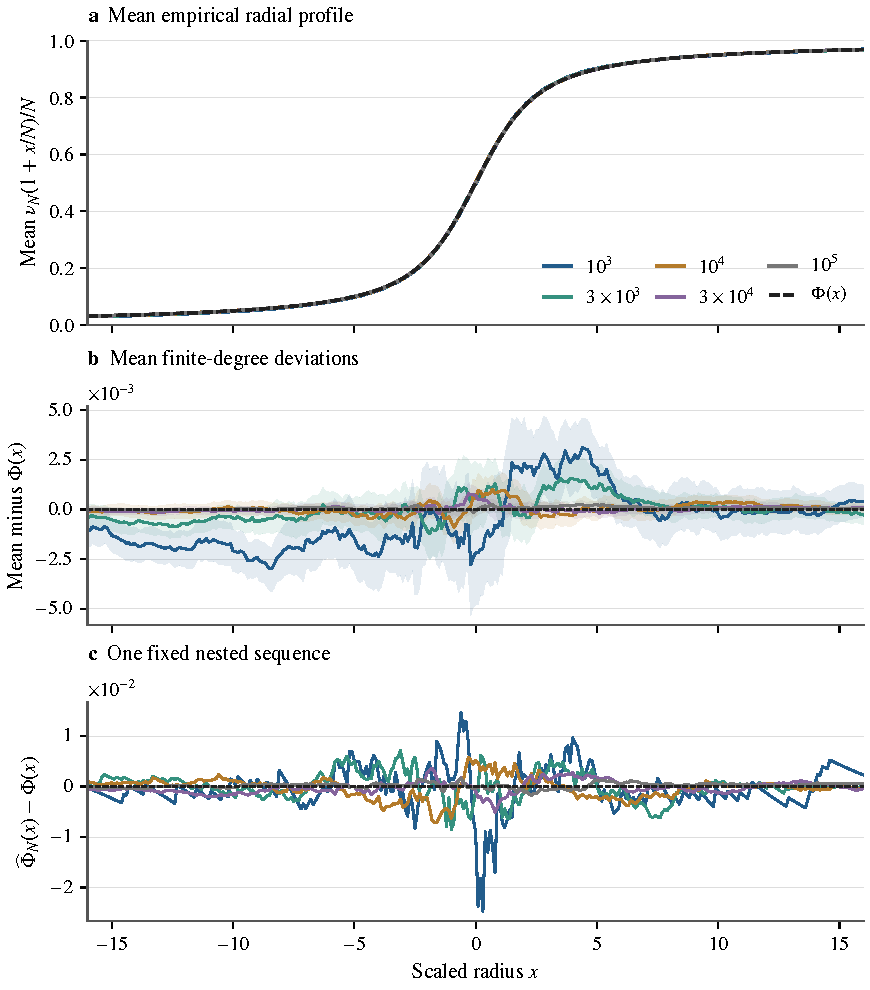
\includegraphics[height=0.6\textheight]{../numerics/publication/figures/radial-profile.pdf}
\caption{Mean empirical radial profile over 77 sequences at five degrees, which
cannot be distinguished from $\Phi$ (a), and its deviations (b, c).}
\label{fig:radial-profile}
\end{figure}



\FloatBarrier
\appendix
\section{Finite constants}\label{sec:constants}\label{app:coefficient-finite}
The main text writes most constants as $C(K)$ or $O_K(\cdot)$. Here we
make them explicit: each is an absolute number times a power of $K+1$
and a factor $e^{bK}$, which gives explicit degree thresholds and lets
Section~\ref{sec:log-rate} take the width $K$ of order $\log N$.
Let $C_*$ be the positive universal constant in
Nazarov--Nishry--Sodin, Corollary~1.2, and let $c_{\rm HW}>0$ be the
constant in Rudelson--Vershynin, Theorem~1.1.
We keep the dependence on both constants in all the bounds below.
We choose, for fixed parameters, the least index beyond which every
displayed inequality holds, so that all degree cutoffs are deterministic.
Table~\ref{tab:const-summary} lists the degree thresholds and the
exceptional probability of each result of the main text, and
Table~\ref{tab:named-constants} lists the named constants.

\begin{table}[!ht]
\centering
\small
\setlength{\tabcolsep}{4pt}
\begin{tabular}{@{}>{\raggedright\arraybackslash}p{0.2\textwidth}
>{\raggedright\arraybackslash}p{0.46\textwidth}
>{\raggedright\arraybackslash}p{0.3\textwidth}@{}}
\toprule
Result & Degree thresholds & Exceptional probability\\
\midrule
\ref{app:const-profile}, Lemma~\ref{lem:profile-rate}
 & $N\ge2K$ & none\\
\ref{app:const-log}, Theorem~\ref{thm:sign-logarithms}
 & $K\ge2$ and $N\ge(160e^{8K})^2$, uniformly for $r\in[1-K/N,1+K/N]$
 & $p_K^*(N)$\\
\ref{app:const-radial}, Corollary~\ref{cor:radial-probability}
 & those of \ref{app:const-log} and $N\ge2K$
 & $4p_K^*(N)$ for \eqref{eq:layer2-radial}, $5p_K^*(N)$ for
 \eqref{eq:radial-count-near-unit}, $5p_2^*(N)$ for its form at $K=2$\\
Lemma~\ref{lem:local-counts}
 & $t_N\le1$ and $N\ge e$ & $N^{-3}$\\
Lemma~\ref{lem:second-derivative}
 & $N\ge\max\{2,(K+1)/3\}$ & $N^{-10}$\\
\ref{app:const-small-derivatives}, Lemma~\ref{lem:small-derivatives}
 & $N\ge(6400e^{8K})^2$, and those of Lemma~\ref{lem:local-counts}
 and \eqref{eq:localization-thresholds}
 & the right-hand side of \eqref{eq:layer2-bad}\\
Lemma~\ref{lem:tails}
 & $j\ge60$ and $N\ge\max\{4,K\}$ & $N^{-10}$\\
Lemma~\ref{lem:isolation-interface}
 & $4aL/N^{3/2}\le1/N$ and $4S_KaL^2N^{-1/2}\sqrt{\log N}\le1$,
 that is, \eqref{eq:localization-thresholds} & none\\
\ref{app:block-bounds}, Section~\ref{sec:layer3}
 & $R\ge|x|+2$, $K\ge R$, $N\ge2R$ and $N\ge(160e^{8R})^2$, which implies
 $N>R$, those of the second to eighth rows at the
 width $K$, where Lemma~\ref{lem:tails} enters with $K+2$ in place of
 $K$ (so that $N\ge\max\{4,K+2\}$), and $j\ge60$
 & \eqref{eq:block-failure}, with $R=2$ and $x=0$ for
 Corollary~\ref{thm:stronglaw}\\
\ref{app:growing-annulus}, Section~\ref{sec:log-rate}
 & the conditions of Table~\ref{tab:growing-annulus}, $j\ge60$, $K\ge2$,
 $A\log N/N\le1$ and $N\ge K+2$
 & \eqref{eq:block-failure}, with $K=K_N$, $R=2$ and $x=0$\\
\ref{app:const-nearby}, Corollary~\ref{cor:crossings}
 & $0<\kappa_*<\min(\kappa,1/64)$ and
 $N^{-1-\kappa}+2a/d_0<N^{-1-\kappa_*}$
 & \eqref{eq:block-failure}, with $R=2$ and the thin-band events of
 \ref{app:const-radial}\\
\bottomrule
\end{tabular}
\caption{The degree thresholds and exceptional probabilities of the
results of the main text, with the subsection of
Appendix~\ref{sec:constants}, where there is one, that treats each. For other coefficient
distributions, Section~\ref{sec:model-constants} enlarges the constants
and adds exceptional probabilities.}
\label{tab:const-summary}
\end{table}

In Table~\ref{tab:named-constants}, $A$, $C_1(K)$, $S_K$ and $\lambda_K$
are the constants of Lemmas~\ref{lem:local-counts}
and~\ref{lem:second-derivative} and of \eqref{eq:jet-eigenvalue}, where
$S_K$ is written $C(K)$ and $\lambda_K$ is written $\lambda$.
The law constants $A_B$, $C_B$, $C_{1,G}$ and $C_{1,B}$ are in
Tables~\ref{tab:law-steinhaus}--\ref{tab:law-bounded}, and $A(B,\eta)$
and $C_1(K,B,\eta)$ in Lemma~\ref{lem:local-counts-general}.
The symbols $A$, $C_0$ and $D_0$ in Corollary~\ref{cor:T3-powers}, $B_0$
in Section~\ref{sec:layer2-models}, and $E_1,E_2$ in
Appendix~\ref{sec:general-estimates} have other meanings.
\begin{table}[p]
\centering
\footnotesize
\setlength{\tabcolsep}{3pt}
\caption{The named constants. Each is at most $C_0(K+1)^pe^{bK}$ with the
listed $(C_0,p,b)$, and the absolute constants have $p=b=0$.}
\label{tab:named-constants}
\begin{tabular}{@{}>{\raggedright\arraybackslash}p{0.1\textwidth}
>{\raggedright\arraybackslash}p{0.27\textwidth}
>{\raggedright\arraybackslash}p{0.13\textwidth}
>{\raggedright\arraybackslash}p{0.14\textwidth}
>{\raggedright\arraybackslash}p{0.28\textwidth}@{}}
\toprule
Constant & Value & $(C_0,p,b)$ & Defined & Used\\
\midrule
$D_K$ & $10(K+1)^2e^{4K}$, and $D_2=90e^8$ & $(10,2,4)$
 & \ref{app:const-profile}
 & \ref{app:const-radial}, \ref{app:block-bounds},
 \ref{app:growing-annulus}, \ref{sec:log-rate},
 Table~\ref{tab:rate-width}\\
$H_K$ & $10^8e^{20(K+1)}$, and $H_2=10^8e^{60}$ & $(H_0,0,20)$
 & \ref{app:const-log}
 & \ref{app:const-radial}, \ref{sec:model-constants},
 \ref{app:growing-annulus}, Table~\ref{tab:rate-width}\\
$C_1(K)$ & $(4A+4K+4)/\log2$, and $C_1(K+2)=(4A+4K+12)/\log2$
 & $(C_{10},1,0)$ for $C_1(K+2)$
 & Lemma~\ref{lem:local-counts}
 & \ref{sec:derivative-detection}, \ref{sec:layer2-models},
 \ref{sec:log-rate}, \ref{app:const-small-derivatives},
 \ref{sec:model-constants}, \ref{app:growing-annulus}\\
$S_K$ & $100e^{K+4}$ & $(S_0,0,1)$
 & Lemma~\ref{lem:second-derivative}
 & \ref{app:const-small-derivatives}, \ref{app:block-bounds},
 \ref{sec:model-constants}, \ref{app:growing-annulus}\\
$\lambda_K$ & $e^{-4K}/80$ & $(1/80,0,-4)$
 & \eqref{eq:jet-eigenvalue}
 & \ref{app:const-small-derivatives}, \ref{sec:model-constants},
 \ref{app:growing-annulus}\\
$D'_K$ & $2^{18}(K+1)S_K^2$ & $(D_0,1,2)$
 & \ref{app:const-small-derivatives}
 & \ref{sec:model-constants}, \ref{app:growing-annulus},
 Proposition~\ref{prop:sparse-exponents}\\
$\mathcal B_K$ & $2000e^{3K}(2/\lambda_K)^{3/2}$ & $(B_0,0,9)$
 & \ref{app:const-small-derivatives}
 & \ref{sec:model-constants}, \ref{app:growing-annulus},
 Proposition~\ref{prop:sparse-exponents}\\
$\mathcal T_K$ & $80e^{4K}/\lambda_K=6400e^{8K}$ & $(6400,0,8)$
 & \ref{app:const-small-derivatives}
 & \ref{sec:model-constants}, \ref{app:growing-annulus},
 Proposition~\ref{prop:sparse-exponents}\\
$V_K$ & $50+3\mathcal B_K+\mathcal T_K$ & $(V_0,0,9)$
 & \ref{app:const-small-derivatives}
 & \ref{sec:model-constants}, \ref{app:growing-annulus}\\
$c_K$ & $9/(1024S_K^2\lambda_K^2)$ & $(Q_0,0,6)$
 & \ref{app:const-small-derivatives}
 & \ref{sec:model-constants}, \ref{app:growing-annulus}\\
$C_K$ & $V_K(D'_K)^2$ & $(C_{\rm bad},2,13)$
 & \ref{app:const-small-derivatives}
 & \eqref{eq:layer2-bad}, \eqref{eq:block-failure},
 \ref{app:growing-annulus}, \ref{sec:log-rate},
 Table~\ref{tab:rate-width}\\
$Z_K$ & $C_1(K+2)(1+D'_Kc_K)$ & $(Z_0,2,8)$
 & \ref{app:const-small-derivatives}
 & \eqref{eq:layer2-bad}, \ref{app:block-bounds},
 \ref{app:growing-annulus}, \ref{sec:log-rate},
 Table~\ref{tab:rate-width}\\
$Z'_K$ & $C_1(K+2)(40+D'_K\mathcal B_K)$ & $(Z'_0,2,11)$
 & \ref{app:const-small-derivatives}
 & \eqref{eq:layer2-bad}, \ref{app:block-bounds},
 \ref{app:growing-annulus}, \ref{sec:log-rate},
 Table~\ref{tab:rate-width}\\
\midrule
$C_*$ & constant of \eqref{eq:layer2-nns}, $C_*\ge1$ &
 & \eqref{eq:layer2-nns}
 & \ref{app:const-log}, $E_1$, $E_2$, \ref{sec:model-constants}\\
$c_{\rm HW}$ & constant of \eqref{eq:HW-signs} &
 & \eqref{eq:HW-signs} & $A$, \ref{sec:model-constants}\\
$A$ & $\max(1,1024\pi/c_{\rm HW})$ &
 & Lemma~\ref{lem:local-counts}
 & $C_1(K)$, $C_{10}$, \ref{sec:log-rate}, \ref{app:growing-annulus}\\
$E_1$ & $\frac52+2e^{1/2}(4eC_*)^6$ &
 & \eqref{eq:layer2-log-split} & $E_0$\\
$E_2$ & $\frac1{16}+e^{1/2}(4eC_*)^6$ &
 & \eqref{eq:layer2-log-split} & $E_0$\\
$H_0$ & $10^8e^{20}$ & & \ref{app:growing-annulus}
 & $E_0$, \eqref{eq:E2-majorants}, \ref{sec:log-rate}\\
$S_0$ & $100e^4$ & & \ref{app:growing-annulus}
 & $D_0$, $Q_0$, Table~\ref{tab:growing-annulus}, \ref{sec:log-rate}\\
$D_0$ & $2^{18}S_0^2$ & & \ref{app:growing-annulus}
 & $C_{\rm bad}$, $Z_0$, $Z'_0$\\
$B_0$ & $2000\cdot160^{3/2}$ & & \ref{app:growing-annulus}
 & $V_0$, $Z'_0$\\
$V_0$ & $50+3B_0+6400$ & & \ref{app:growing-annulus} & $C_{\rm bad}$\\
$Q_0$ & $9\cdot80^2/(1024S_0^2)$ & & \ref{app:growing-annulus} & $Z_0$\\
$C_{10}$ & $(4A+12)/\log2$ & & \ref{app:growing-annulus}
 & $Z_0$, $Z'_0$\\
$C_{\rm bad}$ & $V_0D_0^2$ & & \ref{app:growing-annulus}
 & \eqref{eq:E2-majorants}, \ref{sec:log-rate}\\
$Z_0$ & $C_{10}(1+D_0Q_0)$ & & \ref{app:growing-annulus}
 & \eqref{eq:E2-majorants}, \ref{sec:log-rate}\\
$Z'_0$ & $C_{10}(40+D_0B_0)$ & & \ref{app:growing-annulus}
 & \eqref{eq:E2-majorants}, \ref{sec:log-rate}\\
$E_0$ & $E_1+E_2H_0$ & & \ref{app:growing-annulus}
 & \eqref{eq:E2-majorants}, \ref{sec:log-rate}\\
\bottomrule
\end{tabular}
\end{table}

\subsection{The variance profile}\label{app:const-profile}
For the constant of Lemma~\ref{lem:profile-rate} we set, for an integer
$K\ge2$,
\[
 D_K=10(K+1)^2e^{4K}.
\]
For $N\ge2K$ and $|x|\le K$, Lemma~\ref{lem:profile-rate} and
$1\le9(K+1)^2$ give
\begin{align*}
 \left|\log\sigma_N(1+x/N)-\tfrac12\log N-F(x)\right|
 &\le\frac{K^2+e^{4K}/2}{N}
 \le\frac{(K+1)^2e^{4K}+e^{4K}}{N}\\
 &\le\frac{10(K+1)^2e^{4K}}N=\frac{D_K}N.
\end{align*}

\subsection{Concentration of the angular logarithm}\label{app:const-log}
The one- and two-point bounds give the occupation constant $H_K$ of
Theorem~\ref{thm:sign-logarithms}, and Lemma~\ref{lem:clipping} gives
its error $\varepsilon_K^*(N)$ and exceptional probability $p_K^*(N)$.
Let $K\ge2$ be an integer, set
\[
 H_K=10^8e^{20(K+1)},
\]
and recall that $T=(\log N)/32$ is the clipping level of
Lemma~\ref{lem:clipping}.
The proof of Theorem~\ref{thm:sign-logarithms} uses $N\ge2K$, in
\eqref{eq:layer2-abel} and \eqref{eq:radial-bounds}, $N\ge(160e^{8K})^2$,
so that $40e^{8K}N^{-1/2}\le1/4$ for the covariance matrices of
Section~\ref{sec:h1-rademacher}, and $N\ge e$, in
Lemma~\ref{lem:clipping}. All three hold for $N\ge(160e^{8K})^2$,
since $(160e^{8K})^2=25600e^{16K}$ exceeds $2K$ and $e$.

Let $K\ge2$, $N\ge(160e^{8K})^2$ and $r\in[1-K/N,1+K/N]$.
In \eqref{eq:point-bounds}, the line before the last is $N^{-1/2}$ times
$(42d^{1/4}+16)\cdot46e^{9K}+320e^{8K}$, where the dimension is
$d\in\{2,4\}$, so that $d^{1/4}\le4^{1/4}$. Since
$42\cdot4^{1/4}+16=42\sqrt2+16<75.4$,
$e^{8K}=e^{-K}e^{9K}\le e^{-2}e^{9K}$, $75.4\cdot46=3468.4$ and
$320e^{-2}<44$, we have
\begin{align*}
 (42\cdot4^{1/4}+16)\cdot46e^{9K}+320e^{8K}
 &<75.4\cdot46e^{9K}+320e^{-2}e^{9K}\\
 &<3469e^{9K}+44e^{9K}<4000e^{9K}.
\end{align*}
Hence the one- and two-point differences in \eqref{eq:point-bounds} are
at most $4000e^{9K}N^{-1/2}$ on the retained angles and pairs. As in
\eqref{eq:occupation-bounds}, where the removed sets have measures at
most $2N^{-1/2}$ and $10N^{-1/2}$, we get, uniformly for $t\ge0$,
\[
 |\mathbb EA_t-F_G(t)|\le(2+4000e^{9K})N^{-1/2},\qquad
 |\mathbb EA_t^2-F_G(t)^2|\le(10+4000e^{9K})N^{-1/2}.
\]
Since $12000e^{9K}+14\le12014e^{9K}<10^8e^{20(K+1)}=H_K$ and
$F_G(t)=1-e^{-t^2}$, these bounds, the variance identity of
\eqref{eq:occupation-bounds} and $0\le\mathbb EA_t+F_G(t)\le2$ give
\begin{align}
 |\mathbb EA_t-(1-e^{-t^2})|&\le(2+4000e^{9K})N^{-1/2}
 \le H_KN^{-1/2},\nonumber\\
 \operatorname{Var}(A_t)
 &\le|\mathbb EA_t^2-F_G(t)^2|+2|\mathbb EA_t-F_G(t)|\nonumber\\
 &\le(10+4000e^{9K})N^{-1/2}+2(2+4000e^{9K})N^{-1/2}\nonumber\\
 &=(14+12000e^{9K})N^{-1/2}\le H_KN^{-1/2}.
 \label{eq:layer2-occupation}
\end{align}
We take the deviation for the truncated logarithmic integral, the
parameter $u$ of Theorem~\ref{thm:T1}, to be $N^{-1/16}(\log N)^7$, and
we set
\begin{align*}
 \varepsilon_K^*(N)&=N^{-1/16}(\log N)^7+2H_KTN^{-1/2}\\
 &\quad+e^{1/2}(4eC_*)^6(2N^{-1/16}+H_KN^{-1/2})(\log N)^7+\tfrac32N^{-1/16},\\
 p_K^*(N)&=H_KN^{-3/8}+N^{-12}
 +4H_KT^2N^{-3/8}(\log N)^{-14}.
\end{align*}
Then
\begin{equation}
 \begin{gathered}
 \Prob\{|J_N(r)-\log\sigma_N(r)+\gamma/2|>\varepsilon_K^*(N)\}
 \le p_K^*(N),\\
 \varepsilon_K^*(N)=O_K(N^{-1/16}(\log N)^7).
 \end{gathered}
                                                        \label{eq:layer2-log}
\end{equation}
The first line of \eqref{eq:layer2-log} is Lemma~\ref{lem:clipping} with
$H=H_K$, $C=C_*$, $E=\Omega$ and $B_E=1$, which applies for
$N\ge(160e^{8K})^2$ by \eqref{eq:layer2-occupation}, \eqref{eq:layer2-nns}
and \eqref{eq:layer2-energy}. Its error is $\varepsilon_K^*(N)$, since
$B_E/2+1=\tfrac32$, and its probability bound is $p_K^*(N)$, since
$4T^2=(\log N)^2/256$.
The second line follows from the bound on the error in
Lemma~\ref{lem:clipping}, which at $C=C_*$ and $B_E=1$ reads
\begin{equation}
 \varepsilon_K^*(N)\le E_1N^{-1/16}(\log N)^7+E_2H_KN^{-1/2}(\log N)^7,
 \qquad
 \begin{aligned}
 E_1&=\tfrac52+2e^{1/2}(4eC_*)^6,\\
 E_2&=\tfrac1{16}+e^{1/2}(4eC_*)^6,
 \end{aligned}
 \label{eq:layer2-log-split}
\end{equation}
where $E_1$ and $E_2$ are absolute constants, since $C_*$ is. Only the
second term depends on $K$, and it carries the factor $N^{-1/2}$.

\subsection{Annular mass and thin bands}\label{app:const-radial}
Next we compute the constants of
Corollary~\ref{cor:radial-probability}.
As in its proof, the four secant radii $1\pm K/N$ and $1\pm K/(2N)$ lie
in $[1-K/N,1+K/N]$. Hence
their variance errors are at most $D_K/N$ for $N\ge2K$, by
Section~\ref{app:const-profile}, and each logarithmic error is at most
$\varepsilon_K^*(N)$, outside probability $p_K^*(N)$, for
$N\ge(160e^{8K})^2$, by \eqref{eq:layer2-log}.
Lemma~\ref{lem:annular-mass} at $\eta=1/2$, with
$\varepsilon=\varepsilon_K^*(N)$ and $D=D_K$, then applies outside the
four logarithmic exceptional events, whose union has probability at most
$4p_K^*(N)$, and gives
\begin{equation}
 \frac{\#\{\alpha:||\alpha|-1|>K/N\}}N
 \le\frac{2\log2}{K}+\frac8K\bigl(\varepsilon_K^*(N)+D_K/N\bigr).
 \label{eq:layer2-radial}
\end{equation}

We use all five radii $1+qN^{-1-\kappa}$, $q=-2,\dots,2$, for
$0<\kappa\le1/64$, and $N\ge(160e^{8K})^2$ implies the condition $N\ge4$
of Lemma~\ref{lem:thin-band}. By that lemma with
$\varepsilon=\varepsilon_K^*(N)$, whose hypothesis holds outside the five
events of \eqref{eq:layer2-log} at these radii, for $q=-1,0,1$ the same
sample satisfies
\begin{equation}
 \left|\frac{\nu_N(1+qN^{-1-\kappa})}N-\frac12\right|
 \le2N^{-\kappa}+4\varepsilon_K^*(N)N^\kappa
 \label{eq:radial-count-near-unit}
\end{equation}
outside a union of probability at most $5p_K^*(N)$.
The probabilities of the exceptional events are summable along $N=j^8$,
since $4T^2(\log N)^{-14}=(\log N)^{-12}/256\le1$ for $N\ge e$, so that
the three terms of $p_K^*(j^8)$ are at most $H_Kj^{-3}$, $j^{-96}$ and
$H_Kj^{-3}$.

At $K=2$ we have $H_2=10^8e^{20(2+1)}=10^8e^{60}$, and
$\varepsilon_2^*(N)$ and $p_2^*(N)$ are $\varepsilon_K^*(N)$ and
$p_K^*(N)$ with $10^8e^{60}$ in place of $H_K$, with the degree
threshold $N\ge(160e^{16})^2$. Since the five radii lie in
$[1-2/N,1+2/N]$, \eqref{eq:radial-count-near-unit} holds at $K=2$, with
$\varepsilon_2^*(N)$, outside probability $5p_2^*(N)$.
This form is used in the proof of Corollary~\ref{cor:crossings}.

\subsection{Few small derivatives}\label{app:const-small-derivatives}
We now compute the constants of Lemma~\ref{lem:small-derivatives},
following its proof at the annular width $K$, with the local-count and
tail lemmas at the width $K+2$.

Let $S_K=100e^{K+4}$ be the constant of
Lemma~\ref{lem:second-derivative}, so that
\eqref{eq:sign-second-derivative} holds with $C(K)=S_K$, and let
\[
 C_1(K+2)=\frac{4A+4K+12}{\log2}
\]
be the constant $C_1(K)$ of Lemma~\ref{lem:local-counts} at the width
$K+2$. We set
\begin{align*}
 \lambda_K&=e^{-4K}/80,&
 D'_K&=2^{18}(K+1)S_K^2,\\
 \mathcal B_K&=2000e^{3K}(2/\lambda_K)^{3/2},&
 \mathcal T_K&=80e^{4K}/\lambda_K,\\
 V_K&=50+3\mathcal B_K+\mathcal T_K,&
 c_K&=\frac9{1024S_K^2\lambda_K^2},\\
 C_K&=V_K(D'_K)^2,&
 Z_K&=C_1(K+2)(1+D'_Kc_K),\\
 & & Z'_K&=C_1(K+2)(40+D'_K\mathcal B_K).
\end{align*}
Here $\mathcal B_K$ is the Rai\v{c} bound in the proof of
Lemma~\ref{lem:small-derivatives}, which bounds the normal-approximation
error and the one-point error, and $\mathcal T_K$ bounds the Gaussian
comparison error.

In that proof, the mesh constant must be at most $1/(2S_K)$ for the
bounds \eqref{eq:annular-mesh-test} and at most one for the mesh count. Both conditions hold
for the value $1/(64S_K)$, since $S_K\cdot1/(64S_K)=1/64\le1/2$ and
$S_K\ge1$. With $L=N^{1/64}$, let
\[
 h=\frac1{64S_KNL\sqrt{\log N}}.
\]
We use exactly $\lceil2K/(Nh)\rceil+1$ equally spaced radial rows,
including both endpoints, and $\lceil8\pi/h\rceil$ angles on each row.
This mesh has spacing $h$, and by the count of mesh points in the proof
of Lemma~\ref{lem:small-derivatives}, with $1/(64S_K)$ as its mesh
constant, and $53\cdot64^2=217088<262144=2^{18}$, its total size
satisfies
\begin{align*}
 m&\le53(K+1)(64S_K)^2NL^2\log N=53\cdot64^2(K+1)S_K^2NL^2\log N\\
 &\le2^{18}(K+1)S_K^2NL^2\log N=D'_KNL^2\log N.
\end{align*}
Since $Nh=1/(64S_KL\sqrt{\log N})$,
$N^2h^2\sqrt{\log N}=1/(4096S_K^2L^2\sqrt{\log N})$ and
$1/64+1/8192<1/16$, in \eqref{eq:annular-mesh-test}, with
$C(K)=S_K$ and the mesh constant $1/(64S_K)$, we have
\[
 \frac{Nh}L+\frac{S_K}2N^2h^2\sqrt{\log N}
 =\Bigl(\frac1{64}+\frac1{8192}\Bigr)\frac1{S_KL^2\sqrt{\log N}}
 \le\frac1{16S_KL^2\sqrt{\log N}},
\]
and $2(1+S_K/(64S_K))/L=2(1+1/64)/L=65/(32L)<3/L$.
It follows that the thresholds of Theorem~\ref{thm:T3} at $\tau=h$,
$R=2$ and $M_2=S_KN^{5/2}\sqrt{\log N}$ satisfy
\begin{equation}
 u\le(16S_K)^{-1}L^{-2}(\log N)^{-1/2},
 \qquad v_0\le3/L.
 \label{eq:layer2-meshtest}
\end{equation}
The proof of Lemma~\ref{lem:small-derivatives} uses $N\ge2K$ (in
\eqref{eq:layer2-abel} and for the radial weights), $N\ge K$ (for
$|z|\le2$), $N\ge4$ (for the retained angles on each row), $N\ge e$ (for
$h\le1/N$) and $N^{1/2}\ge6400e^{8K}$ (for the covariance lower bounds
$\lambda_K$ in dimension four and $\lambda_K/2$ in dimension eight).
Since $6400^2e^{16K}$ exceeds $2K$, $4$ and $e$, all of these hold if
\[
 N\ge(6400e^{8K})^2.
\]

By the proof of Lemma~\ref{lem:small-derivatives},
Theorem~\ref{thm:T3} applies with these thresholds, with $p_2=N^{-10}$,
$q_0=C_1(K+2)\log N$, $b_0=40C_1(K+2)\sqrt N\log N$ and $p_0=N^{-3}$, and
with $\lambda=\lambda_K$, $\delta=\delta_*=\mathcal B_KN^{-1/2}$,
$\chi=\mathcal T_KN^{-1/2}$ and $b_*=10N^{-1/2}$.
Since $u^2\le(16S_K)^{-2}L^{-4}(\log N)^{-1}$ and $v_0^2\le9L^{-2}$ by
\eqref{eq:layer2-meshtest}, we have
\[
 \frac{u^2v_0^2}{4\lambda_K^2}
 \le\frac1{4\lambda_K^2}\cdot\frac9{256S_K^2}\cdot\frac{L^{-6}}{\log N}
 =\frac{c_KL^{-6}}{\log N},
\]
so that the line
$u^2v_0^2/(4\lambda^2)+2000e^{3K}(2/\lambda)^{3/2}N^{-1/2}$ of
\eqref{eq:annular-jet-small-ball} gives at $\lambda=\lambda_K$ the
one-point probability
\begin{equation}
 c_KL^{-6}/\log N+\mathcal B_KN^{-1/2}.
 \label{eq:layer2-smallball}
\end{equation}
For a retained separated pair, the covariance of the two indicators in
the proof of Theorem~\ref{thm:T3} is at most
$\delta_*+\chi+2\delta=(3\mathcal B_K+\mathcal T_K)N^{-1/2}$, and
$V_*=(10+3\mathcal B_K+\mathcal T_K)N^{-1/2}\le V_KN^{-1/2}$. Hence, by
\eqref{eq:layer2-smallball} and the bound on $m$,
\begin{equation}
 \mu_*\le D'_K\{c_KNL^{-4}+\mathcal B_KN^{1/2}L^2\log N\},\qquad
 m^2V_*\le V_K(D'_K)^2N^{3/2}L^4(\log N)^2.
 \label{eq:layer2-Z}
\end{equation}
We take $t=NL^{-4}$ in \eqref{eq:T3-general}. By \eqref{eq:layer2-Z}
and $\sqrt N\le N^{1/2}L^2\log N$ for $N\ge e$, we keep the terms with
$NL^{-4}$ apart from those with $N^{1/2}L^2$:
\begin{align*}
 b_0+q_0(\mu_*+t)
 &\le C_1(K+2)(\log N)\bigl[40\sqrt N+NL^{-4}\\
 &\qquad+D'_K\{c_KNL^{-4}+\mathcal B_KN^{1/2}L^2\log N\}\bigr]\\
 &\le Z_KNL^{-4}\log N+Z'_KN^{1/2}L^2(\log N)^2.
\end{align*}
Since $t^2=N^2L^{-8}$ and $L^{12}=N^{3/16}$, \eqref{eq:layer2-Z} gives
\[
 \frac{m^2V_*}{t^2}
 \le V_K(D'_K)^2N^{-1/2}L^{12}(\log N)^2
 =C_KN^{-5/16}(\log N)^2,
\]
and hence, by \eqref{eq:T3-general}, with $p_0=N^{-3}$ the probability
of the exceptional local-count event of Lemma~\ref{lem:local-counts} and
$p_2=N^{-10}$ that of the derivative event of
Lemma~\ref{lem:second-derivative},
\begin{equation}
 \begin{aligned}
 &\Prob\{B_{K,N}>Z_KNL^{-4}\log N+Z'_KN^{1/2}L^2(\log N)^2\}\\
 &\qquad\le N^{-3}+N^{-10}+C_KN^{-5/16}(\log N)^2.
 \end{aligned}
 \label{eq:layer2-bad}
\end{equation}
In this union, the local and derivative events are counted once.
Since $NL^{-4}=N^{15/16}$, $N^{1/2}L^2=N^{17/32}$ and
$N^{17/32}\log N\le N^{15/16}$, the count $B_{K,N}$ is at most
$Z_KN^{15/16}\log N+Z'_KN^{17/32}(\log N)^2\le(Z_K+Z'_K)N^{15/16}\log N$
outside this union. The constant $Z_K$ of the leading term grows like
$(K+1)^2e^{8K}$, and $Z'_K$ like $(K+1)^2e^{11K}$
(Table~\ref{tab:named-constants}). No further threshold on $N$ is
needed here beyond $N\ge(6400e^{8K})^2$ above, the
local-count thresholds $t_N\le1$ and $N\ge e$ of
Lemma~\ref{lem:local-counts}, and the localization thresholds
\eqref{eq:localization-thresholds}.

\subsection{The radial law}\label{app:block-bounds}\label{app:const-moving-radii}
In this subsection we write out in finite form the bounds of the proof of
Theorem~\ref{thm:radial-profile} in Section~\ref{sec:layer3}, and hence
of Corollary~\ref{thm:stronglaw}, which is its case $x=0$ with $R=2$.
Recall that $N=j^8$, $m_j=(j+1)^8-j^8$, $L=N^{1/64}$, $h=N^{-1/64}$ and
$r_N=1+x/N$.
Fix $x$ and integers $R\ge|x|+2$ and $K\ge R$, and let $H_R$, $D_R$,
$\varepsilon_R^*(N)$ and $p_R^*(N)$ be $H_K$, $D_K$, $\varepsilon_K^*(N)$
and $p_K^*(N)$ at the width $R$, with the degree threshold
$N\ge(160e^{8R})^2$.
At $R=2$ these are $\varepsilon_2^*(N)$ and $p_2^*(N)$ of
Section~\ref{app:const-radial}.

Let $a=15e^{2(K+2)}\sqrt{m_j\log N}$ be the tail amplitude of Step~1 of
Section~\ref{sec:layer3}, that is, that of Lemma~\ref{lem:tails} at the
width $K+2$ with $m_{\max}=m_j$. With $M_2=S_KN^{5/2}\sqrt{\log N}$ by
\eqref{eq:sign-second-derivative} and $d_0=N^{3/2}/L$, the localization
conditions $4a/d_0\le1/N$ and $4M_2a\le d_0^2$ of
Table~\ref{tab:unit-conditions} read
\begin{equation}
 4aL/N^{3/2}\le1/N,\qquad4S_KaL^2N^{-1/2}\sqrt{\log N}\le1,
 \label{eq:localization-thresholds}
\end{equation}
since
\[
 \frac{4a}{d_0}=\frac{4aL}{N^{3/2}},\qquad
 \frac{4M_2a}{d_0^2}=\frac{4S_KN^{5/2}\sqrt{\log N}\,aL^2}{N^3}
 =4S_KaL^2N^{-1/2}\sqrt{\log N}.
\]
The second condition implies the first: it gives
$a\le N^{15/32}/(4S_K\sqrt{\log N})$, and then $d_0=N^{95/64}$ gives
$4a/d_0\le N^{-65/64}/(S_K\sqrt{\log N})<1/N$.

By the first line of the bound on $U_N$ in Step~3 of
Section~\ref{sec:layer3}, by \eqref{eq:layer2-radial}, multiplied by
$N$, and by \eqref{eq:layer2-bad}, on the radial and derivative events the
number $U_N$ of unselected roots satisfies
\begin{align}
 U_N&\le\#\{\alpha:f_N(\alpha)=0,\ ||\alpha|-1|>K/N\}+B_{K,N}\nonumber\\
 &\le Z_KN^{15/16}\log N+Z'_KN^{17/32}(\log N)^2\nonumber\\
 &\quad+N\left[\frac{2\log2}{K}+\frac8K\{\varepsilon_K^*(N)+D_K/N\}\right].
 \label{eq:block-unselected}
\end{align}

We apply the logarithmic estimates at $x+qh$, $q=-2,\dots,2$, and
Lemma~\ref{lem:local-radial-secant} at $x+qh$, $q=-1,0,1$, with $R$ in
place of $K$, logarithmic error $\eta_{\log}=\varepsilon_R^*(N)$, profile
error $\varepsilon=D_R/N$, $F'=\Phi$, $M_F=1/2$ and $B_F=1$, since
$0\le\Phi\le1$ and $0\le\Phi'=2\operatorname{Var}_x(t)\le1/2$ by Step~4
of Section~\ref{sec:layer3}, which also implies that
$|\Phi(x+qh)-\Phi(x)|\le|q|h/2$. For $N\ge2R$ we get
\[
 \left|\frac{\nu_N(r_N+qh/N)}N-\Phi(x)\right|
 \le\frac{|q|h}2+\frac h4+\frac RN
 +\frac{2(\varepsilon_R^*(N)+D_R/N)(1+R/N)}h.
\]
Since $|q|h/2+h/4\le2h$ for $|q|\le1$ and $2(1+R/N)\le4$, we obtain
\begin{equation}
 \begin{aligned}
 \left|\frac{\nu_N(r_N+qh/N)}N-\Phi(x)\right|
 &\le\delta_R^*(N),\qquad q=-1,0,1,\\
 \delta_R^*(N)&:=2h+\frac RN+\frac{4(\varepsilon_R^*(N)+D_R/N)}h.
 \end{aligned}\label{eq:E1-local}
\end{equation}
Here the exceptional probability is at most $5p_R^*(N)$, and
$\delta_R^*(N)\to0$. For Corollary~\ref{thm:stronglaw}, at $x=0$ and
$R=2$, this reads
\begin{equation}
 \begin{aligned}
 \left|\frac{\nu_N(1+qN^{-65/64})}N-\frac12\right|
 &\le\delta_2^*(N),\qquad q=-1,0,1,\\
 \delta_2^*(N)&=2N^{-1/64}+\frac2N
 +4\Bigl(\varepsilon_2^*(N)+\frac{D_2}N\Bigr)N^{1/64}.
 \end{aligned}
 \label{eq:block-center-crossings}
\end{equation}

By \eqref{eq:E1-local} with $q=\pm1$, as in \eqref{eq:moving-band}, the
strict band $||\alpha|-r_N|<h/N$ contains at most $2\delta_R^*(N)N$
roots.
This band contains the root of every selected disk whose closure meets
the closed annulus between the circles of radii $r_N$ and $1+x/n$, for
$N\le n\le N+m_j$, once $2a/d_0+|x|m_j/N^2<h/N$, as in Step~4 of
Section~\ref{sec:layer3}. At the width $K\ge R$ this follows from the
thresholds. Indeed, since $d_0=N^{3/2}/L=N^{95/64}$, and
$a\le N^{15/32}/(4S_K\sqrt{\log N})$ by the second condition of
\eqref{eq:localization-thresholds} with $L^2=N^{1/32}$, we have
\[
 N^{65/64}\cdot\frac{2a}{d_0}=2aN^{-15/32}
 \le\frac1{2S_K\sqrt{\log N}}<\frac12,
\]
since $S_K\sqrt{\log N}>1$, and hence, by $N/h=N^{65/64}$ and
\eqref{eq:unit-block-length},
\begin{align*}
 \frac Nh\Bigl(\frac{2a}{d_0}+\frac{|x|m_j}{N^2}\Bigr)
 &=N^{65/64}\cdot\frac{2a}{d_0}+|x|m_jN^{-63/64}\\
 &<\frac12+9|x|N^{-7/64}\le\frac12+\frac12=1,
\end{align*}
since
$18|x|<18R<3e^{7R/4}<160^{7/32}e^{7R/4}\le N^{7/64}$, by $|x|<R$,
$18R<3e^{7R/4}$ for $R\ge2$, $160^{7/32}>3$ and $N\ge(160e^{8R})^2$.
Therefore the number $c(r_N,1+x/n)$ of these disks is at most
$2\delta_R^*(N)N$, and the matching bound of Step~5 of
Section~\ref{sec:layer3} becomes
$|\nu_n(1+x/n)-\nu_N(r_N)|\le2\delta_R^*(N)N+U_N+m_j$.
The chain \eqref{eq:unit-block}, with $\delta_R^*(N)$ in place of
$\varepsilon_N$, then gives
\[
 \left|\frac{\nu_n(1+x/n)}n-\Phi(x)\right|
 \le3\delta_R^*(N)+\frac{U_N}N+\frac{2m_j}{N},
 \qquad N\le n\le N+m_j.
\]

Collecting the exceptional probabilities, we find that the common
exceptional event $E_{K,R,x,j}$ has probability at most
\begin{equation}
 4p_K^*(N)+5p_R^*(N)+N^{-3}+2N^{-10}
                 +C_KN^{-5/16}(\log N)^2.\label{eq:block-failure}
\end{equation}
This union consists of the four radial logarithmic events, used for
$U_N$, the five probe events at the width $R$, used in
\eqref{eq:E1-local}, and the local-count, derivative, mesh-deviation and
maximal-tail events. The shared local-count and derivative events are
counted once each, and a single maximal-tail event controls every degree
in the block. For Corollary~\ref{thm:stronglaw} we take $x=0$ and $R=2$.
For every fixed $K,R$, the series of \eqref{eq:block-failure} over
$N=j^8$ is finite, since its terms are, up to constants, the
probabilities of Table~\ref{tab:unit-events}, where $p_K^*(N)$ and
$p_R^*(N)$ are explicit forms of $\Pi_K(N)$ and $\Pi_R(N)$, and every
exponent of $j$ in the last column of that table is less than $-1$.

\subsection{Other coefficient distributions}\label{sec:model-constants}
This subsection gives the constants with which the other distributions
satisfy (H1)--(H5) in Proposition~\ref{prop:coefficient-transfer}, as
used in the proof of Theorem~\ref{thm:radial-profile} and
Corollary~\ref{thm:stronglaw} for these distributions at the end of
Section~\ref{sec:layer2-models}.
For each distribution we recompute the constants of the sign case from
the inputs that depend on it: its logarithmic-moment constant, its energy
bound, its local-count constant and, for unbounded coefficients, an
envelope on their size.
Tables~\ref{tab:law-steinhaus}, \ref{tab:law-gaussian}
and~\ref{tab:law-bounded} list these constants.

\begin{table}[!ht]
\centering
\small
\begin{tabular}{@{}ll@{}}
\toprule
Input & Value\\
\midrule
Logarithmic moments $(C,\beta)$ & $(C_*,6)$\\
Energy & $E=\Omega$, $B_E=1$, $p_E=0$\\
Occupation constant & $H_K$\\
Local count & $C_1(K+2)$, exceptional probability $N^{-3}$\\
All other constants and thresholds & those of the sign case\\
\bottomrule
\end{tabular}
\caption{Constants for Steinhaus coefficients.}
\label{tab:law-steinhaus}
\end{table}

\paragraph{Steinhaus coefficients.}
These coefficients have the constants of the sign case
(Table~\ref{tab:law-steinhaus}), since their amplitudes have modulus
one, so that conditional signs yield the same $C_*$ and $C_1(K+2)$.

\begin{table}[!ht]
\centering
\small
\begin{tabular}{@{}>{\raggedright\arraybackslash}p{0.27\textwidth}
>{\raggedright\arraybackslash}p{0.69\textwidth}@{}}
\toprule
Input & Value\\
\midrule
Logarithmic moments $(C,\beta)$ & $(16,6)$\\
Energy & $E=\{V\le B_E\}$, $B_E=2$,
 $p_E=\exp[-3N/(32e^{6K})]$\\
Occupation constant & $H_K$\\
Local count & $C_{1,G}(K+2)=C_1(K+2)+2/\log2
 =(4A+4(K+2)+6)/\log2=(4A+4K+14)/\log2$,
 exceptional probability $N^{-3}+\exp[-3(N+1)/32]$\\
Small derivatives & $Z_{K,G}=C_{1,G}(K+2)(1+D'_Kc_K)$,
 $Z'_{K,G}=C_{1,G}(K+2)(40+D'_K\mathcal B_K)$; $D'_K$, $c_K$,
 $\mathcal B_K$, $V_K$ and $C_K=V_K(D'_K)^2$ unchanged\\
Derivative and tails & amplitudes of the sign case,
 $\lceil N^4\rceil\le2N^4$ boundary samples, on the envelope event
 $\max_{k\le2N}|g_k|\le N$ of probability at least
 $1-2(2N+1)e^{-N^2/2}$\\
Thresholds & $N\ge(160e^{8K})^2$, $N\ge e^2$, $\rho\le2$, and those of
 the sign case\\
\bottomrule
\end{tabular}
\caption{Constants for standard real and complex Gaussian coefficients.}
\label{tab:law-gaussian}
\end{table}

\paragraph{Real and complex Gaussian coefficients.}
By the proof of Proposition~\ref{prop:coefficient-transfer}, with
Lemma~\ref{lem:local-counts-gauss} for the local count, standard complex
Gaussian coefficients have the constants of the real ones
(Table~\ref{tab:law-gaussian}).

The choice $(C,\beta)=(16,6)$ is valid, since $(16p)^p\le(16p)^{6p}$ for
$p\ge1$, so that, by \eqref{eq:layer2-gaussianlog}, the logarithmic
moments satisfy \eqref{eq:layer2-nns} with $16$ in place of $C_*$.
In the proof of Proposition~\ref{prop:coefficient-transfer}, the Gaussian
occupation constants $2+320e^{8K}$ and $14+960e^{8K}$ are at most $H_K$,
since $2+320e^{8K}<14+960e^{8K}\le974e^{9K}<10^8e^{20(K+1)}=H_K$, so that
\eqref{eq:layer2-occupation} holds for these coefficients.
Hence Lemma~\ref{lem:clipping} applies with $H=H_K$, $C=16$,
$E=\{V\le B_E\}$ and $B_E=2$, where $V=\int|X_r|^2\dd\mu$ as in
Proposition~\ref{prop:coefficient-transfer}, and $\Prob(E^c)\le p_E$ by
\eqref{eq:layer2-gaussianenergy}.

This is the computation of Section~\ref{app:const-log} with $C_*$
replaced by $16$, $B_E=1$ by $2$ and the term $p_E$ added: since
$4e\cdot16=64e$, $B_E/2+1=2$ and $4T^2=(\log N)^2/256$, it gives, for
$N\ge(160e^{8K})^2$ and $r\in[1-K/N,1+K/N]$,
\begin{align*}
 &\Prob\bigl\{|J_N(r)-\log\sigma_N(r)+\gamma/2|
 >N^{-1/16}(\log N)^7+2H_KTN^{-1/2}\\
 &\qquad\quad+e^{1/2}(64e)^6(2N^{-1/16}+H_KN^{-1/2})(\log N)^7+2N^{-1/16}\bigr\}\\
 &\quad\le H_KN^{-3/8}+N^{-12}
 +\frac{H_K}{256}N^{-3/8}(\log N)^{-12}+p_E.
\end{align*}
For these coefficients, the error and the probability on the two sides of
this display replace $\varepsilon_K^*(N)$ and $p_K^*(N)$ at each radius in
\eqref{eq:layer2-radial}, \eqref{eq:radial-count-near-unit},
\eqref{eq:block-unselected}, \eqref{eq:block-center-crossings},
\eqref{eq:block-failure} and \eqref{eq:E1-local}, and in the radial
thresholds of Section~\ref{app:const-radial}.

The bounds of Lemmas~\ref{lem:second-derivative} and~\ref{lem:tails} keep
the amplitudes of the sign case on the envelope event, by the proof of
Proposition~\ref{prop:coefficient-transfer}: with $\lceil N^4\rceil$
samples in place of $\lceil N^3\rceil$, the derivative bounds gain the
factor $N$ and the sample spacing loses it.
The thresholds $N\ge e^2$ and $\rho\le2$ imply the conditions $N\ge4$ and
$\rho\le2$ of the interpolation step in the proof of Lemma~\ref{lem:tails}.
In $Z_K$ and $Z'_K$ we replace $C_1(K+2)$ by $C_{1,G}(K+2)$, while the
other constants of Section~\ref{app:const-small-derivatives} remain upper
bounds, since the normal approximation is exact. On the common
coefficient-envelope event, the bound \eqref{eq:layer2-bad} is then
replaced by
\begin{multline*}
 \Prob\{B_{K,N}>Z_{K,G}NL^{-4}\log N+Z'_{K,G}N^{1/2}L^2(\log N)^2\}\\
 \le N^{-3}+\exp[-3(N+1)/32]+N^{-10}+C_KN^{-5/16}(\log N)^2.
\end{multline*}
All other exceptional probabilities are those of the sign case.

\begin{table}[!ht]
\centering
\small
\begin{tabular}{@{}>{\raggedright\arraybackslash}p{0.27\textwidth}
>{\raggedright\arraybackslash}p{0.69\textwidth}@{}}
\toprule
Input & Value\\
\midrule
Logarithmic moments $(C,\beta)$ & $(C_B,6)$, with
 $C_B=2\{C_*+\max(\tfrac12\log2,\log B)+1\}$\\
Energy & $E=\{V\ge1/2\}$, $B_E=B^2$,
 $p_H=\exp[-N/(2B^4e^{6K})]$\\
Occupation constant & $H_{K,B}=(1+B^3)H_K$\\
Derivative and mesh & $S_{K,B}=BS_K$, $D'_{K,B}=B^2D'_K$,
 $\mathcal B_{K,B}=B^3\mathcal B_K$, $c_{K,B}=c_K/B^2$; $\lambda_K$ and
 $\mathcal T_K$ unchanged\\
Tail amplitude & $Ba$, with $a=15e^{2(K+2)}\sqrt{m_j\log N}$\\
Local count & $A_B=\max(1,2048\pi B^2/c_{\rm HW})$,
 $C_{1,B}(K+2)=(4A_B+4(K+2)+4+\log B)/\log2$,
 exceptional probability $N^{-3}+\exp[-(N+1)/(2B^4)]$\\
Small derivatives & $V_{K,B}$, $C_{K,B}$, $Z_{K,B}$, $Z'_{K,B}$: the
 formulas for $V_K$, $C_K$, $Z_K$, $Z'_K$ with these constants and
 $C_{1,B}(K+2)$\\
Thresholds & $A_B\log N/N\le1$, $N\ge e^2$, and the enlarged thresholds
 below\\
\bottomrule
\end{tabular}
\caption{Constants for a bounded centrally symmetric distribution with
$\mathbb E|\xi_0|^2=1$ and $|\xi_0|\le B$.}
\label{tab:law-bounded}
\end{table}

\paragraph{Centrally symmetric bounded coefficients.}
Assume that the coefficient distribution is nondegenerate and centrally
symmetric, as defined in Section~\ref{par:central-symmetry}.
We normalize $\mathbb E|\xi_0|^2=1$ and assume $|\xi_0|\le B$, so that
$B\ge1$.
We use $V$, $E=\{V\ge1/2\}$, $J_N$ and $C_B$ as in
Proposition~\ref{prop:coefficient-transfer} and its proof, and the
constants of Table~\ref{tab:law-bounded}, where $a$ is the tail
amplitude of Step~1 of Section~\ref{sec:layer3}.
The local-count constant is that of Lemma~\ref{lem:local-counts-bounded}
with $K+2$ in place of $K$, and the conditional trace event adds
$\exp[-(N+1)/(2B^4)]$ to its exceptional probability.
Since $\mathcal B_{K,B}=B^3\mathcal B_K$, $2/\lambda_K=160e^{4K}$,
$(160e^{4K})^{3/2}=160^{3/2}e^{6K}$, $80e^{4K}/\lambda_K=6400e^{8K}$,
$D'_{K,B}=B^2D'_K$, $(D'_K)^2=2^{36}(K+1)^2S_K^4$ and
$S_K^4=10^8e^{4K+16}$, and since $D'_{K,B}c_{K,B}=D'_Kc_K$ and
$D'_{K,B}\mathcal B_{K,B}=B^5D'_K\mathcal B_K$,
\begin{align*}
 V_{K,B}&=50+3\mathcal B_{K,B}+\mathcal T_K
 =50+6000B^3e^{3K}(2/\lambda_K)^{3/2}+\frac{80e^{4K}}{\lambda_K}\\
 &=50+6000\cdot160^{3/2}B^3e^{9K}+6400e^{8K},\\
 C_{K,B}&=V_{K,B}(D'_{K,B})^2=B^4V_{K,B}(D'_K)^2\\
 &=2^{36}\cdot10^8B^4(K+1)^2e^{4K+16}V_{K,B},\\
 Z_{K,B}&=C_{1,B}(K+2)(1+D'_{K,B}c_{K,B})=C_{1,B}(K+2)(1+D'_Kc_K),\\
 Z'_{K,B}&=C_{1,B}(K+2)(40+D'_{K,B}\mathcal B_{K,B})
 =C_{1,B}(K+2)(40+B^5D'_K\mathcal B_K).
\end{align*}
For the occupation bounds, the constant $c_B$ of the proof of
Proposition~\ref{prop:coefficient-transfer} satisfies, as in
Section~\ref{app:const-log} with the factor $B^3$ on the first term only
and with $B\ge1$ in the last step,
\[
 c_B=(42\cdot4^{1/4}+16)\cdot46B^3e^{9K}+320e^{8K}
 <3469B^3e^{9K}+44e^{9K}<4000B^3e^{9K}.
\]
Hence, by $B^3e^{9K}\ge1$, $12014<10^8$ and $9K<20(K+1)$, the occupation
constants $2+c_B<14+3c_B$ of that proof satisfy
$14+3c_B<14+12000B^3e^{9K}\le12014B^3e^{9K}<B^3H_K<H_{K,B}$, so that
\eqref{eq:layer2-occupation} holds with $H_{K,B}$ in place of $H_K$.
Hence Lemma~\ref{lem:clipping} applies with $H=H_{K,B}$, $C=C_B$,
$E=\{V\ge1/2\}$ and $B_E=B^2$, by the moment bound on $E$ in
Proposition~\ref{prop:coefficient-transfer} and since $V\le B^2$.
With $B_E/2+1=B^2/2+1$ and $4T^2=(\log N)^2/256$, its error is
\begin{align*}
 \varepsilon_{K,B}^*(N)
 &=N^{-1/16}(\log N)^7+2H_{K,B}TN^{-1/2}\\
 &\quad +e^{1/2}(4eC_B)^6(2N^{-1/16}+H_{K,B}N^{-1/2})(\log N)^7
 +(B^2/2+1)N^{-1/16},
\end{align*}
and it gives
\begin{align*}
 &\Prob\{|J_N(r)-\log\sigma_N(r)+\gamma/2|>\varepsilon_{K,B}^*(N)\}
 \le H_{K,B}N^{-3/8}+N^{-12}\\
 &\qquad+\frac{H_{K,B}}{256}N^{-3/8}(\log N)^{-12}
 +\exp[-N/(2B^4e^{6K})],
\end{align*}
where the last term is the probability of $E^c$ from
\eqref{eq:layer2-boundedenergy}.
As in the real Gaussian case, $\varepsilon_{K,B}^*(N)$ and the right-hand
side of the last display replace $\varepsilon_K^*(N)$ and $p_K^*(N)$ at
each radius.
Similarly, by the proof of Proposition~\ref{prop:coefficient-transfer}
with the deviation $t=NL^{-4}$, the bound \eqref{eq:layer2-bad} is
replaced by
\begin{multline*}
 \Prob\{B_{K,N}>Z_{K,B}NL^{-4}\log N+Z'_{K,B}N^{1/2}L^2(\log N)^2\}\\
 \le N^{-3}+\exp[-(N+1)/(2B^4)]+N^{-10}+C_{K,B}N^{-5/16}(\log N)^2.
\end{multline*}
We require $A_B\log N/N\le1$ and $N\ge e^2$, and all previous thresholds
with the enlarged constants.
Since $S_{K,B}\cdot Ba=B^2S_Ka$, these are
\begin{align*}
 &N\ge(6400e^{8K})^2,\qquad N\ge2K,\\
 &4BaL/N^{3/2}\le1/N,\qquad
  4B^2S_KaL^2N^{-1/2}\sqrt{\log N}\le1,
\end{align*}
together with the thresholds $N\ge\max\{2,(K+1)/3\}$, $j\ge60$ and
$N\ge\max\{4,K+2\}$, which do not change.
These inequalities hold eventually for each fixed distribution, with
cutoffs that depend on $B$.

If $\Prob(\xi_0=0)>0$, the trailing-zero allowance $\lceil D\log N\rceil$,
with $D>4/|\log\Prob(\xi_0=0)|$, and the bound
$N^{-D|\log\Prob(\xi_0=0)|}$ on the probability of its exceptional event
at each degree are those of the proof of
Theorem~\ref{thm:radial-profile} and Corollary~\ref{thm:stronglaw} for
other distributions in Section~\ref{sec:layer2-models}, which also
treats the initial zero multiplicity and the actual degrees in
Corollary~\ref{cor:T4-two-radii}.

\subsection{Bounds for a growing annulus}\label{app:growing-annulus}
In this subsection we compute the constants of the proof in
Section~\ref{sec:log-rate}, at the width $K=K_N$, where
$K_N=\lfloor(\log N)/128-\log\log N\rfloor$ is the width of that
section, with $N=j^8$ and $L=N^{1/64}$ as before, and with the
local-count and tail lemmas at the width $K+2$.
The following bounds hold whenever the displayed deterministic conditions
hold.
Set
\begin{align*}
 H_0&=10^8e^{20},&S_0&=100e^4,&D_0&=2^{18}S_0^2,\\
 B_0&=2000\cdot160^{3/2},&V_0&=50+3B_0+6400,&
 Q_0&=\frac{9\cdot80^2}{1024S_0^2},\\
 A&=\max(1,1024\pi/c_{\rm HW}),&C_{10}&=(4A+12)/\log2,&
 C_{\rm bad}&=V_0D_0^2,\\
 Z_0&=C_{10}(1+D_0Q_0),&Z'_0&=C_{10}(40+D_0B_0),&
 E_0&=E_1+E_2H_0,
\end{align*}
where $E_1$ and $E_2$ are the absolute constants of
\eqref{eq:layer2-log-split}.
These constants are independent of $K,N$.
By the definitions we have, for $K\ge0$,
\begin{align*}
 H_K&=H_0e^{20K},&S_K&=S_0e^K,&D'_K&=D_0(K+1)e^{2K},\\
 \mathcal B_K&=B_0e^{9K},&\mathcal T_K&=6400e^{8K},&V_K&\le V_0e^{9K},\\
 c_K&=Q_0e^{6K},&C_1(K+2)&\le C_{10}(K+1),&
 C_K&\le C_{\rm bad}(K+1)^2e^{13K},\\
 Z_K&\le Z_0(K+1)^2e^{8K},&Z'_K&\le Z'_0(K+1)^2e^{11K}.
\end{align*}
Indeed, the first three hold since $H_K=10^8e^{20}e^{20K}$,
$S_K=100e^4e^K$ and $D'_K=2^{18}(K+1)S_K^2=2^{18}S_0^2(K+1)e^{2K}$. For the
others we use $1/\lambda_K=80e^{4K}$, so that $2/\lambda_K=160e^{4K}$ and
$\mathcal T_K=80e^{4K}\cdot80e^{4K}=6400e^{8K}$, and, for the bounds,
$e^{8K}\le e^{9K}$, $1\le(K+1)e^{bK}$, $4K\le(4A+12)K$ and
$C_1(K+2)=(4A+4(K+2)+4)/\log2$:
\begin{align*}
 \mathcal B_K&=2000e^{3K}(160e^{4K})^{3/2}=2000\cdot160^{3/2}e^{9K}
 =B_0e^{9K},\\
 V_K&=50+3B_0e^{9K}+6400e^{8K}\le(50+3B_0+6400)e^{9K}=V_0e^{9K},\\
 c_K&=\frac{9\cdot80^2e^{8K}}{1024S_0^2e^{2K}}=Q_0e^{6K},\\
 C_1(K+2)&=\frac{4A+4K+12}{\log2}
 \le\frac{(4A+12)(K+1)}{\log2}=C_{10}(K+1),\\
 C_K&=V_K(D'_K)^2
 \le V_0e^{9K}\cdot D_0^2(K+1)^2e^{4K}
 =C_{\rm bad}(K+1)^2e^{13K},\\
 Z_K&=C_1(K+2)(1+D'_Kc_K)
 \le C_{10}(K+1)\{1+D_0Q_0(K+1)e^{8K}\}\\
 &\le Z_0(K+1)^2e^{8K},\\
 Z'_K&=C_1(K+2)(40+D'_K\mathcal B_K)
 \le C_{10}(K+1)\{40+D_0B_0(K+1)e^{11K}\}\\
 &\le Z'_0(K+1)^2e^{11K}.
\end{align*}

These are the forms $C_0(K+1)^pe^{bK}$ of
Table~\ref{tab:named-constants}, and the following lemma evaluates such
a form at $K=K_N$.

\begin{lemma}[Constants at the growing width]\label{lem:growing-width}
Let $N\ge e$ and $K_N\ge0$, and let $X_K\le C_0(K+1)^pe^{bK}$ with
$C_0\ge0$, $p\ge0$ and $b\ge0$. Then
\[
 X_{K_N}\le C_0(K_N+1)^pN^{b/128}(\log N)^{-b},
\]
and if moreover $K_N+1\le\log N$, then
$X_{K_N}\le C_0(\log N)^pN^{b/128}(\log N)^{-b}$.
\end{lemma}

\begin{proof}
By the floor, $K_N\le(\log N)/128-\log\log N$, and hence, since $b\ge0$
and $\log N\ge1$,
\[
 e^{bK_N}\le N^{b/128}(\log N)^{-b}\le N^{b/128},\qquad b\ge0.
\]
This gives the first bound, and the second follows since
$0<K_N+1\le\log N$ and $p\ge0$.
\end{proof}

By Lemma~\ref{lem:growing-width} with the forms above, keeping the
factor $(K+1)^p$ and, only for $Z_K$, the factor $(\log N)^{-8}$, we get
for $N\ge e$
\begin{align}
 \varepsilon_K^*(N)&\le E_0N^{-1/16}(\log N)^7,\nonumber\\
 D_K/N&\le10(K+1)^2N^{-31/32},\nonumber\\
 p_K^*(N)&\le H_0N^{-7/32}+N^{-12}
 +\frac{H_0}{256}N^{-7/32}(\log N)^{-12},\nonumber\\
 C_KN^{-5/16}(\log N)^2
 &\le C_{\rm bad}(K+1)^2N^{-27/128}(\log N)^2,\nonumber\\
 Z_KN^{-1/16}\log N
 &\le Z_0(K+1)^2(\log N)^{-7},\nonumber\\
 Z'_KN^{-15/32}(\log N)^2
 &\le Z'_0(K+1)^2N^{-49/128}(\log N)^2.
                                                        \label{eq:E2-majorants}
\end{align}
By Lemma~\ref{lem:growing-width} with $b=20$, we have
$H_K=H_0e^{20K}\le H_0N^{5/32}$, and $5/32-1/2=-11/32$ and
$5/32-3/8=-7/32$. By \eqref{eq:layer2-log-split} and
$N^{-11/32}\le N^{-1/16}$, the first line follows from
\[
 \varepsilon_K^*(N)
 \le E_1N^{-1/16}(\log N)^7+E_2H_0N^{-11/32}(\log N)^7
 \le E_0N^{-1/16}(\log N)^7.
\]
The second line follows from
$D_K/N=10(K+1)^2e^{4K}N^{-1}\le10(K+1)^2N^{1/32-1}=10(K+1)^2N^{-31/32}$.
Since $4T^2=(\log N)^2/256$, the third line follows from
\begin{align*}
 p_K^*(N)&=H_KN^{-3/8}+N^{-12}
 +\frac{H_K}{256}N^{-3/8}(\log N)^{-12}\\
 &\le H_0N^{-7/32}+N^{-12}
 +\frac{H_0}{256}N^{-7/32}(\log N)^{-12}.
\end{align*}
By the bounds on $C_K$, $Z_K$ and $Z'_K$ above, and
Lemma~\ref{lem:growing-width} with $b=13$, $b=8$ and $b=11$, the last
three lines follow from $13/128-5/16=-27/128$,
$e^{8K}N^{-1/16}\le(\log N)^{-8}$ and $11/128-15/32=-49/128$.

The caps on $K/\log N$ in Table~\ref{tab:rate-width} are $\beta/b$ in
its first part and $(\beta-1/8)/b$ in its second, where $b$ is the
exponent of the named constant of the row in
Table~\ref{tab:named-constants}, plus $2$ for the factor
$e^{2(K+2)}=e^4e^{2K}$ of $a$ in the two rows with $a$, and $b=16$ for
$(6400e^{8K})^2$.

Each ratio in Table~\ref{tab:growing-annulus} tends to zero, and the
indicated condition holds once the ratio is at most one.
Indeed, at $K=K_N$ every ratio other than $2K/N$ is a constant times
powers of $K_N+1\le\log N$ and of $\log N$, times a negative power of
$N$, and $2K_N/N\le2(\log N)/N$. These rates are compared in
Section~\ref{sec:log-rate}.
\begin{table}[!htbp]
\centering
\small
\begin{tabular}{>{\raggedright\arraybackslash}p{0.32\textwidth}p{0.61\textwidth}}
\toprule
Condition & Sufficient ratio bound\\
\midrule
$(160e^{8K})^2\le N$, $(6400e^{8K})^2\le N$ & $6400^2N^{-7/8}$\\
$2K\le N$ & $2K/N$\\
Taylor localization inequality
 & $180S_0e^4(\log N)N^{-1/128}$\\
$2a/d_0<N^{-65/64}$
 & $90e^4\sqrt{\log N}\,N^{-1/64}$\\
\bottomrule
\end{tabular}
\caption{Sufficient ratio bounds for the degree conditions at the width
$K=K_N$.}
\label{tab:growing-annulus}
\end{table}
We require the last ratio to be strictly below one. The condition
$4a/d_0\le1/N$ follows from the Taylor localization inequality, as shown
after \eqref{eq:localization-thresholds}.

We obtain the ratios of the table by dividing each condition by its
right-hand side and substituting the bounds above. For the first row,
since $160<6400$ and by Lemma~\ref{lem:growing-width} with $b=16$,
\[
 \frac{(6400e^{8K})^2}N=6400^2e^{16K}N^{-1}\le6400^2N^{1/8-1}
 =6400^2N^{-7/8}.
\]
The last two rows, for the inequality
$4S_KaL^2N^{-1/2}\sqrt{\log N}\le1$ of Taylor localization in
\eqref{eq:localization-thresholds}, which is $4M_2a\le d_0^2$, and for
the strict band $N^{65/64}\cdot2a/d_0<1$, are computed in the proof of
Theorem~\ref{thm:log-rate} from \eqref{eq:unit-radius} and
\eqref{eq:unit-parameters}, with $180S_0e^4=18000e^8$ and the
exponents $7/16+1/32-1/2=-1/32$, $3/128-1/32=-1/128$,
$7/16-15/32=-1/32$ and $2/128-1/32=-1/64$. They use the bound
$m_j\le9N^{7/8}$ of \eqref{eq:unit-block-length} and the bound
$a\le45e^4e^{2K}N^{7/16}\sqrt{\log N}$ of \eqref{eq:unit-amplitude},
where $e^{2(K+2)}=e^4e^{2K}$.
The small-derivative lemma adds no ratio to the table, since its
thresholds are $N\ge(6400e^{8K})^2$, those of
Lemma~\ref{lem:local-counts} and \eqref{eq:localization-thresholds}.

We also impose
\[
 j\ge60,\qquad K\ge2,\qquad A\log N/N\le1,\qquad N\ge K+2.
\]
These conditions are eventual.
Beyond a fixed cutoff, the secant and probe radii belong to their
required annuli.
In this way we obtain all local-count, covariance, tail, localization
and radial cutoffs used in the proof.

The proof in Section~\ref{sec:log-rate} bounds the number $U_N$ of
unselected roots at $K=K_N$, in place of \eqref{eq:block-unselected}, by
\begin{equation}
 U_N\le N\Bigl[\frac1{K-1}+4\Bigl(\varepsilon_K^*(N)+\frac{D_K}N\Bigr)\Bigr]
 +Z_KN^{15/16}\log N+Z'_KN^{17/32}(\log N)^2,
 \label{eq:rate-unselected}
\end{equation}
outside the four radial events at the radii $1\pm(K_N-1)/N$ and
$1\pm K_N/N$ and the event of \eqref{eq:layer2-bad}.
Its probes are those of \eqref{eq:block-center-crossings}, at the fixed
width $2$, so that the probe error at the unit circle is at most
$\delta_2^*(N)$ and the crossing count at most $2\delta_2^*(N)N$.
By \eqref{eq:unit-block} at $x=0$, with $\delta_2^*(N)$ in place of
$\varepsilon_N$ as in Section~\ref{app:block-bounds}, and
\eqref{eq:rate-unselected} divided by $N$, the bound that we
use for the logarithmic rate is, for $N\le n\le N+m_j$,
\begin{align}
 \left|\frac{\nu_n(1)}n-\frac12\right|
 &\le3\delta_2^*(N)+\frac{U_N}N+\frac{2m_j}{N}\nonumber\\
 &\le3\Bigl(2N^{-1/64}+\frac2N
   +4\Bigl(\varepsilon_2^*(N)+\frac{D_2}N\Bigr)N^{1/64}\Bigr)
   +\frac1{K_N-1}\nonumber\\
 &\quad+4\Bigl(\varepsilon_{K_N}^*(N)+\frac{D_{K_N}}N\Bigr)
   +Z_{K_N}N^{-1/16}\log N\nonumber\\
 &\quad+Z'_{K_N}N^{-15/32}(\log N)^2+\frac{2m_j}{N}.
 \label{eq:E2-final}
\end{align}
Here $\varepsilon_{K_N}^*(N)$, $H_{K_N}=10^8e^{20(K_N+1)}$,
$D_{K_N}=10(K_N+1)^2e^{4K_N}$, $Z_{K_N}$ and $Z'_{K_N}$ are
$\varepsilon_K^*(N)$, $H_K$, $D_K$, $Z_K$ and $Z'_K$ at $K=K_N$, and
$D_2=90e^8$.
For this bound, the exceptional probability is \eqref{eq:block-failure}
with $K=K_N$, $R=2$ and $x=0$, where $C_{K_N}=V_{K_N}(D'_{K_N})^2$ and
$p_{K_N}^*(N)$ is the function $p_K^*(N)$ at $K=K_N$. By the third and
fourth lines of \eqref{eq:E2-majorants}, with $4H_0/256=H_0/64$, its terms
$4p_{K_N}^*(N)+C_{K_N}N^{-5/16}(\log N)^2$ are bounded as in the proof of
Theorem~\ref{thm:log-rate}.
By Lemma~\ref{lem:growing-width}, through \eqref{eq:E2-majorants}, every
term in \eqref{eq:E2-final} other than $1/(K_N-1)$ is $o(1/\log N)$, as
in Section~\ref{sec:log-rate}, since $K_N+1\le\log N$ and
$m_j/N\le9N^{-1/8}$.

\subsection{Nearby circles}\label{app:const-nearby}
Finally, we compute the constants of the proof of
Corollary~\ref{cor:crossings} in Section~\ref{sec:nearby-circles}.
For a target exponent $\kappa>0$, we choose a wider band with
\[
 0<\kappa_*<\min(\kappa,1/64),
\]
as does the choice $\kappa_*=\min(\kappa/2,1/128)$ in that proof.
Then the band $||z|-1|<N^{-1-\kappa_*}$ contains the circles
$|z|=1\pm N^{-1-\kappa}$, and $\kappa_*$ lies in the range
$0<\kappa\le1/64$ of the thin-band estimate of
Section~\ref{app:const-radial}.
We impose
\[
 N^{-1-\kappa}+2a/d_0<N^{-1-\kappa_*},
\]
where $2a/d_0$ is the radius of the selected disks of Step~2 of
Section~\ref{sec:layer3}. As in the proof of
Corollary~\ref{cor:crossings}, this condition places every good annular
root whose disk meets one of the circles in the band.
By the form of \eqref{eq:radial-count-near-unit} at $K=2$ in
Section~\ref{app:const-radial}, with $\kappa_*$ in place of $\kappa$,
\[
 \left|\frac{\nu_N(1+qN^{-1-\kappa_*})}N-\frac12\right|
 \le2N^{-\kappa_*}+4\varepsilon_2^*(N)N^{\kappa_*},\qquad q=-1,0,1,
\]
outside probability $5p_2^*(N)$.
Since $p_2^*(N)$ does not depend on the thin-band exponent, the
exceptional probability of the block is \eqref{eq:block-failure} with
$R=2$, where the term $5p_2^*(N)$ now bounds these five thin-band events
in place of the five probe events.

\section{General concentration and counting estimates}
\label{sec:general-estimates}\label{sec:layer1}

Let $(a_k)_{k\geq0}$ be a sequence of random complex coefficients on one
probability space, and put
\[
 f_N(z)=\sum_{k=0}^N a_kz^k.
\]
The same coefficient sequence is used for all degrees, and in particular
$\deg f_N\leq N$ when $f_N$ is nonzero.
Let $\sigma_N(r)>0$ be deterministic, and write
\[
 J_N(r)=\int_{\mathbb T}\log|f_N(re^{i\theta})|\dd\mu(\theta),
\]
where $\mu$ is the normalized angular measure. Deterministic counting
statements concern nonzero polynomials, and in probabilistic
applications we include the case of an identically zero polynomial in an
explicit exceptional event.

\subsection{Angular occupation and logarithmic integrals}

\begin{namedhypothesis}[One- and two-point occupation bounds]\phantomsection\label{hyp:occupation}
For fixed $N,r$, we set
\[
 X(\theta)=\frac{f_N(re^{i\theta})}{\sigma_N(r)}.
\]
Let $G$ have density $\pi^{-1}e^{-|z|^2}$ on $\C$. We set
\[
 F_G(t)=\Prob(|G|\leq t)=1-e^{-t^2}.
\]
There are measurable exceptional sets
$E_1\subset\mathbb T$, $E_2\subset\mathbb T^2$ with
$\mu(E_1)\leq\eta_1$, $(\mu\otimes\mu)(E_2)\leq\eta_2$, such that, for
all $s,t\geq0$,
\[
 \left|\Prob(|X(\theta)|\leq t)-F_G(t)\right|\leq\delta_1
       \quad(\theta\notin E_1),
\]
\[
 \left|\Prob(|X(\theta)|\leq s,|X(\phi)|\leq t)-F_G(s)F_G(t)\right|
       \leq\delta_2\quad((\theta,\phi)\notin E_2).
\]
\end{namedhypothesis}
In the two-point bound we compare with a pair of independent standard
complex Gaussians, and if the normal approximation yields a correlated
Gaussian pair, then $\delta_2$ includes the error of the comparison with
this independent pair.

\begin{namedhypothesis}[Logarithmic moments and energy]\phantomsection\label{hyp:logenergy}
For fixed constants $C>0$, $\beta>0$, and for all real $p>1$,
\begin{equation}
 \E\int_{\mathbb T}|\log|X(\theta)||^p\dd\mu(\theta)
       \leq(Cp)^{\beta p}. \label{eq:log-moment-bound}
\end{equation}
We will also use the following eventwise bound on an event
$E_H$ with $\Prob(E_H^c)\leq p_H$:
\begin{equation}
 \E\left[\boldsymbol1_{E_H}
       \int_{\mathbb T}|\log|X(\theta)||^p\dd\mu(\theta)\right]
       \leq(Cp)^{\beta p}\qquad(p>1). \label{eq:event-log-moment-bound}
\end{equation}
Here the expectation is the integral over $E_H$. We evaluate the
integrand only on that event. This also defines the eventwise bound when the angular
integral is infinite on $E_H^c$.
The exact angular energy identity is
\begin{equation}
 \int_{\mathbb T}|X(\theta)|^2\dd\mu(\theta)=1
       \quad\hbox{almost surely}. \label{eq:exact-angular-energy}
\end{equation}
The upper-energy probability bound is
\begin{equation}
 \Prob\left(\int_{\mathbb T}|X(\theta)|^2\dd\mu(\theta)>B_E\right)
       \leq p_E \qquad(B_E>0). \label{eq:angular-energy-tail}
\end{equation}
\end{namedhypothesis}
The full bound \eqref{eq:log-moment-bound} is the case
$E_H=\Omega$ and $p_H=0$ of \eqref{eq:event-log-moment-bound}.
We use the tail form \eqref{eq:angular-energy-tail} when the coefficient
moduli are random, and under \eqref{eq:exact-angular-energy} we can take
$B_E=1$, $p_E=0$.
For the coefficient distributions of Sections~\ref{sec:concentration}
and~\ref{sec:layer2-models}, these logarithmic bounds hold for every
$p\ge1$ (see \eqref{eq:layer2-nns}, \eqref{eq:layer2-gaussianlog} and
Proposition~\ref{prop:coefficient-transfer}), but in the proof of
Theorem~\ref{thm:T1} we use them only for $p=2q\ge2$.

\begin{theorem}[Logarithmic integral concentration]\label{thm:T1}
Assume the \hyperref[hyp:occupation]{one- and two-point occupation bounds},
the eventwise logarithmic bound \eqref{eq:event-log-moment-bound},
and the energy bound \eqref{eq:angular-energy-tail}. We set
\[
 d_1=\delta_1+\eta_1,\qquad d_2=\delta_2+\eta_2,
 \qquad v=d_2+2d_1.
\]
For all $T>0$, $u>0$, $b>0$, $q\geq1$, and $\lambda>1$, we set
\begin{align}
 \eta_{\log}={}&u+2Td_1+\lambda(2Cq)^\beta
        \sqrt{e^{-2T}+d_1+b}
        +(B_E/2+1)e^{-2T}, \label{eq:T1-error}\\
 p_{\rm fail}={}&v/b^2+\lambda^{-2q}+4T^2v/u^2+p_E+p_H. \label{eq:T1-failure}
\end{align}
Then
\[
 \Prob\left(\left|J_N(r)-\log\sigma_N(r)
                   -\E\log|G|\right|>\eta_{\log}\right)\leq p_{\rm fail},
 \qquad \E\log|G|=-\gamma/2.
\]
The same conclusion holds if, in place of the occupation bounds,
$|\E A_t-F_G(t)|\leq d_1$ and $\operatorname{Var}(A_t)\leq v$ for all
$t\geq0$ and some $d_1,v\geq0$, where
$A_t=\mu\{\theta:|X(\theta)|\leq t\}$. If moreover
$\int_{\mathbb T}|X|^2\dd\mu\leq B_E$ on $E_H$, then $p_E+p_H$ in
\eqref{eq:T1-failure} may be replaced by $\Prob(E_H^c)$.
\end{theorem}

\begin{proof}
The idea is to clip the logarithm at $\pm T$, to estimate the mean and
the variance of the clipped integral by the occupation bounds, and to
control the lower tail that the clipping removes by the logarithmic
moments and the occupation bound at $e^{-T}$, and the upper tail by the
energy bound. Table~\ref{tab:T1-events} lists the five exceptional events,
one for each term of \eqref{eq:T1-failure}.

We set
$A_t=\int_{\mathbb T}\boldsymbol1_{\{|X(\theta)|\leq t\}}\dd\mu(\theta)$.
By Tonelli's theorem, we have
\begin{align*}
 \E A_t
 &=\int_{\mathbb T}\Prob(|X(\theta)|\leq t)\dd\mu(\theta),\\
 \E A_t^2
 &=\E\int_{\mathbb T^2}
      \boldsymbol1_{\{|X(\theta)|\leq t\}}
      \boldsymbol1_{\{|X(\phi)|\leq t\}}\dd\mu(\theta)\dd\mu(\phi)\\
 &=\int_{\mathbb T^2}
      \Prob(|X(\theta)|\leq t,|X(\phi)|\leq t)
         \dd\mu(\theta)\dd\mu(\phi).
\end{align*}
By these identities and the
\hyperref[hyp:occupation]{one- and two-point occupation bounds}, with $s=t$
in the second, and since the probabilities and $F_G(t)$ lie in $[0,1]$, we
have, for every $t\geq0$,
\begin{align*}
 |\E A_t-F_G(t)|
 &=\left|\int_{\mathbb T}\bigl(\Prob(|X(\theta)|\leq t)-F_G(t)\bigr)
       \dd\mu(\theta)\right|\\
 &\leq\int_{\mathbb T\setminus E_1}\delta_1\dd\mu
       +\int_{E_1}1\dd\mu
 \leq\delta_1+\mu(E_1)
 \leq d_1,\\
 |\E A_t^2-F_G(t)^2|
 &=\left|\int_{\mathbb T^2}\bigl(\Prob(|X(\theta)|\leq t,|X(\phi)|\leq t)
       -F_G(t)^2\bigr)\dd(\mu\otimes\mu)\right|\\
 &\leq\int_{\mathbb T^2\setminus E_2}\delta_2\dd(\mu\otimes\mu)
       +\int_{E_2}1\dd(\mu\otimes\mu)
 \leq\delta_2+(\mu\otimes\mu)(E_2)
 \leq d_2.
\end{align*}
Since both $\E A_t$ and $F_G(t)$ belong to $[0,1]$, we have
\begin{gather*}
 |(\E A_t)^2-F_G(t)^2|
 =|\E A_t-F_G(t)|\,|\E A_t+F_G(t)|
 \leq2d_1,\\
 \operatorname{Var}(A_t)
 =\E A_t^2-(\E A_t)^2
 \leq|\E A_t^2-F_G(t)^2|+|(\E A_t)^2-F_G(t)^2|
 \leq d_2+2d_1
 =v.
\end{gather*}
From here on, the occupation bounds enter only through the bounds
$|\E A_t-F_G(t)|\leq d_1$ and $\operatorname{Var}(A_t)\leq v$, which
proves the first variant in the statement.

Since $F_G(e^{-T})=1-\exp(-e^{-2T})\leq e^{-2T}$, taking $t=e^{-T}$ in
these bounds and applying Chebyshev's inequality, we obtain
\begin{align*}
 \E A_{e^{-T}}
 &\leq F_G(e^{-T})+d_1
 \leq e^{-2T}+d_1,\\
 \Prob(A_{e^{-T}}>e^{-2T}+d_1+b)
 &\leq\Prob(A_{e^{-T}}-\E A_{e^{-T}}>b)
 \leq\frac{\operatorname{Var}(A_{e^{-T}})}{b^2}
 \leq\frac v{b^2}.
\end{align*}
We call the event $\{A_{e^{-T}}>e^{-2T}+d_1+b\}$ the Chebyshev event for
$A_{e^{-T}}$.

On $E_H$, we set
$U=\int_{\mathbb T}|\log|X(\theta)||^2\dd\mu(\theta)$.
By Jensen's inequality and \eqref{eq:event-log-moment-bound} with $p=2q$,
we have
\begin{align*}
 U^q
 &=\left(\int_{\mathbb T}|\log|X(\theta)||^2\dd\mu(\theta)\right)^q
 \leq\int_{\mathbb T}|\log|X(\theta)||^{2q}\dd\mu(\theta),\\
 \E[\boldsymbol1_{E_H}U^q]
 &\leq\E\left[\boldsymbol1_{E_H}
       \int_{\mathbb T}|\log|X(\theta)||^{2q}\dd\mu(\theta)\right]
 \leq(2Cq)^{2\beta q}.
\end{align*}
Applying Markov's inequality to $U^q$ on $E_H$, we get
\[
 \Prob\{\omega\in E_H:U>\lambda^2(2Cq)^{2\beta}\}
 \leq\frac{\E[\boldsymbol1_{E_H}U^q]}
              {\lambda^{2q}(2Cq)^{2\beta q}}
 \leq\frac{(2Cq)^{2\beta q}}{\lambda^{2q}(2Cq)^{2\beta q}}
 =\lambda^{-2q}.
\]
We call the event on the left the Markov event for $U$.

We now truncate the logarithm and set
$\ell_T(z)=\max(-T,\min(T,\log|z|))$ and
$L_T=\int_{\mathbb T}\ell_T(X)\dd\mu$.
For every $z\in\C$, including $z=0$, we have the layer-cake identity
\[
 \ell_T(z)=T-\int_{-T}^T\boldsymbol1_{\{|z|\leq e^\tau\}}\dd\tau,
\]
since the set of $\tau\in[-T,T]$ with $|z|\leq e^\tau$ is
$[\max(-T,\log|z|),T]$ if $\log|z|\leq T$ (with $\log0=-\infty$), and is
empty otherwise.
By the layer-cake identity at $z=X(\theta)$ and at $z=G$, Tonelli's
theorem and $\Prob(|G|\leq e^\tau)=F_G(e^\tau)$, we have
\begin{align*}
 L_T
 &=\int_{\mathbb T}\left(T-\int_{-T}^T
         \boldsymbol1_{\{|X(\theta)|\leq e^\tau\}}\dd\tau\right)\dd\mu(\theta)
 =T-\int_{-T}^T A_{e^\tau}\dd\tau,\\
 \E L_T-\E\ell_T(G)
 &=\int_{-T}^T\bigl(F_G(e^\tau)-\E A_{e^\tau}\bigr)\dd\tau,\\
 L_T-\E L_T
 &=-\int_{-T}^T(A_{e^\tau}-\E A_{e^\tau})\dd\tau.
\end{align*}
By these identities, the bounds $|\E A_t-F_G(t)|\leq d_1$ and
$\operatorname{Var}(A_t)\leq v$, and the Cauchy--Schwarz inequality, we
have
\begin{align*}
 |\E L_T-\E\ell_T(G)|
 &\leq\int_{-T}^T|\E A_{e^\tau}-F_G(e^\tau)|\dd\tau
 \leq2Td_1,\\
 |\operatorname{Cov}(A_{e^\tau},A_{e^{\tau'}})|
 &\leq\sqrt{\operatorname{Var}(A_{e^\tau})\operatorname{Var}(A_{e^{\tau'}})}
 \leq v,
\end{align*}
and hence, by Fubini's theorem, which applies since
$|A_{e^\tau}-\E A_{e^\tau}|\leq1$,
\begin{align*}
 &\operatorname{Var}(L_T)
 =\E\left(\int_{-T}^T(A_{e^\tau}-\E A_{e^\tau})\dd\tau\right)^2\\
 &\quad=\int_{-T}^T\int_{-T}^T
       \E[(A_{e^\tau}-\E A_{e^\tau})(A_{e^{\tau'}}-\E A_{e^{\tau'}})]
       \dd\tau\dd\tau'\\
 &\quad=\int_{-T}^T\int_{-T}^T
       \operatorname{Cov}(A_{e^\tau},A_{e^{\tau'}})\dd\tau\dd\tau'
 \leq\int_{-T}^T\int_{-T}^T
       |\operatorname{Cov}(A_{e^\tau},A_{e^{\tau'}})|\dd\tau\dd\tau'
 \leq4T^2v.
\end{align*}
Applying Chebyshev's inequality again, we get
\[
 \Prob(|L_T-\E L_T|>u)
 \leq\frac{\operatorname{Var}(L_T)}{u^2}
 \leq\frac{4T^2v}{u^2}.
\]
We call the event on the left the Chebyshev event for $L_T$.

On $E_H$, outside the Chebyshev event for $A_{e^{-T}}$ and the Markov
event for $U$, by the Cauchy--Schwarz inequality we bound the negative
truncation error by
\begin{align*}
 \int_{\{|X|<e^{-T}\}}(-\log|X|-T)\dd\mu
 &\leq\int_{\{|X|<e^{-T}\}}|\log|X||\dd\mu\\
 &\leq\left(\int_{\mathbb T}|\log|X||^2\dd\mu\right)^{1/2}
       \left(\int_{\mathbb T}
         \boldsymbol1_{\{|X|<e^{-T}\}}\dd\mu\right)^{1/2}\\
 &\leq\sqrt{UA_{e^{-T}}}
 \leq\lambda(2Cq)^\beta\sqrt{e^{-2T}+d_1+b}.
\end{align*}
On the energy event $\{\int_{\mathbb T}|X|^2\dd\mu\leq B_E\}$, by
Tonelli's theorem applied to
$(y-T)_+=\int_T^\infty\boldsymbol1_{\{y>\tau\}}\dd\tau$ at $y=\log|X|$
and by Markov's inequality for $\mu$, we bound the positive truncation
error by
\begin{align*}
 \int_{\{|X|>e^T\}}(\log|X|-T)\dd\mu
 &=\int_T^\infty\mu\{|X|>e^\tau\}\dd\tau
 \leq\int_T^\infty e^{-2\tau}\Bigl(\int_{\mathbb T}|X|^2\dd\mu\Bigr)\dd\tau\\
 &\leq\int_T^\infty B_E e^{-2\tau}\dd\tau
 =\frac{B_E}2e^{-2T}.
\end{align*}
For the Gaussian tails,
$\int_T^\infty\Prob(|G|<e^{-\tau})\dd\tau$ and
$\int_T^\infty\Prob(|G|>e^\tau)\dd\tau$ are at most
$\frac12e^{-2T}$ by \eqref{eq:gaussian-log-tails}.
On $E_H$, outside the Markov event for $U$, the integral
$\int_{\mathbb T}\log|X|\dd\mu$ is finite, since
$\int_{\mathbb T}|\log|X||^2\dd\mu=U\leq\lambda^2(2Cq)^{2\beta}$. Since
\[
 |\ell_T(z)-\log|z||=(-\log|z|-T)_++(\log|z|-T)_+,
\]
on $E_H$ and on the energy event, outside the Chebyshev event for
$A_{e^{-T}}$ and the Markov event for $U$, it follows from the layer-cake
identity, the two truncation bounds and the two Gaussian tail bounds that
\begin{align*}
 \left|\int_{\mathbb T}\log|X|\dd\mu-L_T\right|
 &\leq\int_{\mathbb T}|\log|X|-\ell_T(X)|\dd\mu\\
 &=\int_{\{|X|<e^{-T}\}}(-\log|X|-T)\dd\mu
      +\int_{\{|X|>e^T\}}(\log|X|-T)\dd\mu\\
 &\leq\lambda(2Cq)^\beta\sqrt{e^{-2T}+d_1+b}+\frac{B_E}2e^{-2T},\\
 |\E\ell_T(G)-\E\log|G||
 &\leq\E|\ell_T(G)-\log|G||
 =\E(-\log|G|-T)_++\E(\log|G|-T)_+\\
 &=\int_T^\infty\Prob(|G|<e^{-\tau})\dd\tau
       +\int_T^\infty\Prob(|G|>e^\tau)\dd\tau
 \leq e^{-2T}.
\end{align*}

\begin{table}[!htbp]
\centering
\begin{tabular}{@{}lll@{}}
\toprule
Exceptional event & Defined by & Probability at most\\
\midrule
Chebyshev event for $A_{e^{-T}}$ & $A_{e^{-T}}>e^{-2T}+d_1+b$ & $v/b^2$\\
Markov event for $U$ & $\omega\in E_H$, $U>\lambda^2(2Cq)^{2\beta}$
 & $\lambda^{-2q}$\\
Chebyshev event for $L_T$ & $|L_T-\E L_T|>u$ & $4T^2v/u^2$\\
Complement of the energy event & $\int_{\mathbb T}|X|^2\dd\mu>B_E$
 & $p_E$\\
Complement of $E_H$ & & $p_H$\\
\bottomrule
\end{tabular}
\caption{The exceptional events in the proof of Theorem~\ref{thm:T1}.
The sum of the bounds on their probabilities is
\eqref{eq:T1-failure}.}
\label{tab:T1-events}
\end{table}
Finally, $J_N(r)-\log\sigma_N(r)=\int\log|X|\dd\mu$, and outside the five
exceptional events of Table~\ref{tab:T1-events}, by the previous display
and the bounds on $|L_T-\E L_T|$ and $|\E L_T-\E\ell_T(G)|$, we have
\begin{align*}
 &\left|\int\log|X|\dd\mu-\E\log|G|\right|
 \leq\left|\int\log|X|\dd\mu-L_T\right|
       +|L_T-\E L_T|\\
 &\qquad+|\E L_T-\E\ell_T(G)|
       +|\E\ell_T(G)-\E\log|G||\\
 &\qquad\leq\lambda(2Cq)^\beta\sqrt{e^{-2T}+d_1+b}+\frac{B_E}2e^{-2T}
       +u+2Td_1+e^{-2T}
 =\eta_{\log}.
\end{align*}
Under \eqref{eq:exact-angular-energy} and \eqref{eq:log-moment-bound} the
last two events are absent. If $\int_{\mathbb T}|X|^2\dd\mu\leq B_E$ on $E_H$,
then the complement of the energy event is contained in $E_H^c$, so that
the last two events have probability at most $\Prob(E_H^c)$ together,
which proves the second variant in the statement. By \eqref{eq:event-log-moment-bound},
the logarithmic integral is finite almost surely on $E_H$, even for
polynomials with roots on the integration circle.
Since $|G|^2$ has the exponential distribution with mean one,
\eqref{eq:euler-centering} gives $\E\log|G|=-\gamma/2$.
\end{proof}

\begin{remark}[Polynomial choices of parameters]\label{rem:T1-powers}
If $d_1\leq D N^{-a}$ and $v\leq V N^{-a}$, choose
$T=t\log N$, $b=N^{-2t}$, $u=N^{-w}$, and $q=c\log N\geq1$.
Under \eqref{eq:log-moment-bound} and \eqref{eq:exact-angular-energy},
we may take $p_H=0$, $B_E=1$ and $p_E=0$. With $\lambda=e$, so that
$\lambda(2Cq)^\beta=e(2Cc\log N)^\beta$, the terms of
\eqref{eq:T1-error} and \eqref{eq:T1-failure}, other than $u=N^{-w}$ and
$p_E=p_H=0$, satisfy
\begin{align*}
 2Td_1&\leq2t(\log N)DN^{-a},\qquad
 (B_E/2+1)e^{-2T}=\tfrac32N^{-2t},\\
 e^{-2T}+d_1+b&\leq N^{-2t}+DN^{-a}+N^{-2t}=2N^{-2t}+DN^{-a},\\
 v/b^2&\leq VN^{-a}/N^{-4t}=VN^{4t-a},\qquad
 \lambda^{-2q}=e^{-2c\log N}=N^{-2c},\\
 4T^2v/u^2&\leq4t^2(\log N)^2VN^{-a}/N^{-2w}=4t^2V(\log N)^2N^{2w-a}.
\end{align*}
By substituting these bounds, we get
\[
 \eta_{\log}\leq N^{-w}+2tD(\log N)N^{-a}
  +e(2Cc\log N)^\beta\sqrt{2N^{-2t}+DN^{-a}}
  +\tfrac32N^{-2t},
\]
\[
 p_{\rm fail}\leq VN^{4t-a}+N^{-2c}
       +4t^2V(\log N)^2N^{2w-a}.
\]
The failure terms tend to zero when $4t<a$ and $2w<a$.
For $N=j^s$, the three failure terms are
\[
 Vj^{-s(a-4t)},\qquad j^{-2cs},\qquad
 4t^2Vs^2(\log j)^2j^{-s(a-2w)},
\]
and they are summable if
\[
 s(a-4t)>1,\qquad 2cs>1,\qquad s(a-2w)>1.
\]
In particular, take $a=1/2$, $t=w=1/32$, $c=6$, $\beta=6$ and $s=8$.
Then $s(a-4t)=8(\frac12-\frac18)=3$, $2cs=2\cdot6\cdot8=96$ and
$s(a-2w)=8(\frac12-\frac1{16})=\frac72$ all exceed one, and for $N\geq e$,
\begin{align*}
 \eta_{\log}
 &\leq N^{-1/32}+\frac D{16}(\log N)N^{-1/2}
  +e(12C\log N)^6\sqrt{2N^{-1/16}+DN^{-1/2}}
  +\tfrac32N^{-1/16}\\
 &\leq\Bigl(\frac52+\frac D{16}+e(12C)^6\sqrt{2+D}\Bigr)
       N^{-1/32}(\log N)^6,
\end{align*}
by the bound on $\eta_{\log}$ above with $2tD=D/16$, $2Cc=12C$,
$2t=1/16$ and $w=1/32$, and by $\log N\geq1$ and
$N^{-1/2}\leq N^{-1/16}\leq N^{-1/32}$.
So we get an error bounded by the above constant times
$N^{-1/32}(\log N)^6$ and a summable failure on $j^8$. For large enough
degree the error is at most $N^{-1/32}(\log N)^7$, with a deterministic
threshold depending on the fixed constant: it suffices that $\log N$ is at
least the above constant. We use the moments of the angular
logarithmic norm in \eqref{eq:log-moment-bound}.
The proof of Lemma~\ref{lem:clipping} takes instead
$u=N^{-1/32}(\log N)^7$, $q=\lceil\log N\rceil$ and
$\lambda=(2e\log N/q)^6\log N\ge e^6\log N$,
for which $\lambda(2Cq)^6=(4eC)^6(\log N)^7$ and
$\lambda^{-2q}\le N^{-12}$. The choice $q=6\log N$, $\lambda=e$ above
gives the same failure bound $N^{-2c}=N^{-12}$ with
$\lambda(2Cq)^6=e(12C\log N)^6$. The extra factor $\log N$ in $\lambda$
is the difference between the exponents $7$ and $6$.
\end{remark}

\subsection{A local radial secant estimate}

\begin{lemma}[Local approximation of radial counts]\label{lem:local-radial-secant}
Let $f_N$ be a nonzero polynomial of degree at most $N$, and let
$\sigma_N(r)>0$ be deterministic. Suppose that the function $F_N(x)$,
equal to $\log\sigma_N(1+x/N)$ minus a centering independent of $x$,
satisfies $|F_N(x)-F(x)|\leq\varepsilon$ on $[-K,K]$.
Suppose also $|F'|\leq B_F$ and
$|F'(x)-F'(y)|\leq M_F|x-y|$ there.
Suppose the three logarithmic deviations
\[
 \left|J_N(1+y/N)-\log\sigma_N(1+y/N)-\E\log|G|\right|,
 \qquad y=x-h,x,x+h,
\]
are at most $\eta_{\log}$ outside their respective exceptional events.
If $h>0$ and $|x|+h\leq K<N$, then outside the union of those three events,
\begin{equation}
 \left|\frac{\nu_N(1+x/N)}N-F'(x)\right|
 \leq\frac{M_Fh}{2}+\frac{B_FK}{N}
       +\frac{2(\eta_{\log}+\varepsilon)(1+K/N)}h. \label{eq:T2-moving}
\end{equation}
In particular an
error $\eta_{\log}+\varepsilon\leq N^{-1/32}(\log N)^7$, with $h=N^{-\kappa}$,
$0<\kappa\leq1/64$, gives convergence to $F'(0)$ uniformly for
deterministic $|x|\leq h$.
\end{lemma}

\begin{proof}
By Jensen's formula, $\nu_N(r)/N$ lies between two secant slopes of
$J_N$ in the variable $N\log\rho$, one on each side of $r$, and the idea
is to replace $J_N$ by $F$ at the three probe points, up to a constant
which cancels, and then to compare the secant slopes of $F$ with $F'(x)$.
This leads to three errors, which come from the curvature of $F$, the
change of the denominators, and the deviations of $J_N$ from $F$ at the
probe points.

Let $r=1+x/N$ and set
\[
 d_-=N\log\frac{r}{r-h/N},\qquad
 d_+=N\log\frac{r+h/N}{r}.
\]
Since $|x|+h\leq K<N$, we have $r-h/N=1+(x-h)/N\geq1-K/N>0$.
By the integral form \eqref{eq:jensen-integral} of Jensen's formula,
in which $\nu_N$ counts the roots in the closed disk, and since $\nu_N$ is
nondecreasing, we have
\begin{align*}
 J_N(r)-J_N(r-h/N)
 &=\int_{r-h/N}^r\frac{\nu_N(\rho)}\rho\dd\rho
 \leq\nu_N(r)\log\frac r{r-h/N}
 =\frac{\nu_N(r)d_-}N,\\
 J_N(r+h/N)-J_N(r)
 &=\int_r^{r+h/N}\frac{\nu_N(\rho)}\rho\dd\rho
 \geq\nu_N(r)\log\frac{r+h/N}r
 =\frac{\nu_N(r)d_+}N.
\end{align*}
Dividing by $d_\pm>0$, we obtain the Jensen bounds
\[
 \frac{J_N(r)-J_N(r-h/N)}{d_-}
 \leq\frac{\nu_N(r)}N
 \leq\frac{J_N(r+h/N)-J_N(r)}{d_+}.
\]
Since $N\log(1+u/N)$ has derivative $1/(1+u/N)$ in $u$, we have
\begin{align*}
 d_-&=N\log(1+x/N)-N\log\bigl(1+(x-h)/N\bigr)
 =\int_{x-h}^x\frac{\mathrm du}{1+u/N},\\
 d_+&=N\log\bigl(1+(x+h)/N\bigr)-N\log(1+x/N)
 =\int_x^{x+h}\frac{\mathrm du}{1+u/N}.
\end{align*}
Since $|x|+h\leq K<N$, every $u\in[x-h,x+h]$ satisfies
$0<1-K/N\leq1+u/N\leq1+K/N$, and taking reciprocals and integrating over
an interval of length $h$, we obtain
\begin{gather*}
 \frac1{1+K/N}\leq\frac1{1+u/N}\leq\frac1{1-K/N},\qquad
 \frac h{1+K/N}\leq d_\pm\leq\frac h{1-K/N},\\
 1-\frac KN\leq\frac h{d_\pm}\leq1+\frac KN,\qquad
 \left|\frac h{d_\pm}-1\right|\leq\frac KN.
\end{gather*}

Since $F'$ is Lipschitz on $[-K,K]$, which contains $x\pm t$ for
$0\leq t\leq h$, for the ordinary secants we have
\begin{align*}
 \left|\frac{F(x+h)-F(x)}h-F'(x)\right|
 &=\left|\frac1h\int_0^h\bigl(F'(x+t)-F'(x)\bigr)\dd t\right|\\
 &\leq\frac1h\int_0^h M_Ft\dd t
 =\frac{M_Fh}2,\\
 \left|\frac{F(x)-F(x-h)}h-F'(x)\right|
 &=\left|\frac1h\int_0^h\bigl(F'(x-t)-F'(x)\bigr)\dd t\right|\\
 &\leq\frac1h\int_0^h M_Ft\dd t
 =\frac{M_Fh}2.
\end{align*}
Each ordinary secant has absolute value at most $B_F$, since it is the
mean of $F'$ over an interval in $[-K,K]$.
Replacing its denominator $h$ by $d_\pm$ multiplies it by $h/d_\pm$, and
\begin{align*}
 \left|\frac{F(x+h)-F(x)}{d_+}-\frac{F(x+h)-F(x)}h\right|
 &=\left|\frac{F(x+h)-F(x)}h\right|\,\left|\frac h{d_+}-1\right|\\
 &\leq B_F\left|\frac h{d_+}-1\right|
 \leq\frac{B_FK}N,\\
 \left|\frac{F(x)-F(x-h)}{d_-}-\frac{F(x)-F(x-h)}h\right|
 &=\left|\frac{F(x)-F(x-h)}h\right|\,\left|\frac h{d_-}-1\right|\\
 &\leq B_F\left|\frac h{d_-}-1\right|
 \leq\frac{B_FK}N.
\end{align*}
Let $c$ be the centering, so that $F_N(x)=\log\sigma_N(1+x/N)-c$.
For $y=x-h,x,x+h$, which lie in $[-K,K]$, we have
\begin{align*}
 &J_N(1+y/N)-\E\log|G|-c-F(y)\\
 &\quad=\bigl\{J_N(1+y/N)-\log\sigma_N(1+y/N)-\E\log|G|\bigr\}
        +\bigl\{F_N(y)-F(y)\bigr\}.
\end{align*}
The constant $\E\log|G|+c$ does not depend on $y$, so that it cancels from
each secant, and outside the exceptional event at $y$ the first brace is
at most $\eta_{\log}$ in absolute value and the second is at most
$\varepsilon$. Since
$r\pm h/N=1+(x\pm h)/N$, by subtracting the identity at two neighboring
probe points we obtain
\begin{align*}
 \bigl|J_N(r+h/N)-J_N(r)-\bigl(F(x+h)-F(x)\bigr)\bigr|
 &\leq2(\eta_{\log}+\varepsilon),\\
 \bigl|J_N(r)-J_N(r-h/N)-\bigl(F(x)-F(x-h)\bigr)\bigr|
 &\leq2(\eta_{\log}+\varepsilon).
\end{align*}
By the lower bound $d_\pm\geq h/(1+K/N)$, the secant error is therefore at
most $2(\eta_{\log}+\varepsilon)/d_\pm\leq2(\eta_{\log}+\varepsilon)(1+K/N)/h$.
Adding the three errors to the Jensen bounds, we obtain
\begin{align*}
 \frac{\nu_N(r)}N
 &\leq\frac{J_N(r+h/N)-J_N(r)}{d_+}
 \leq\frac{F(x+h)-F(x)}{d_+}+\frac{2(\eta_{\log}+\varepsilon)(1+K/N)}h\\
 &\leq\frac{F(x+h)-F(x)}h+\frac{B_FK}N
      +\frac{2(\eta_{\log}+\varepsilon)(1+K/N)}h\\
 &\leq F'(x)+\frac{M_Fh}2+\frac{B_FK}N
      +\frac{2(\eta_{\log}+\varepsilon)(1+K/N)}h,\\
 \frac{\nu_N(r)}N
 &\geq\frac{J_N(r)-J_N(r-h/N)}{d_-}
 \geq\frac{F(x)-F(x-h)}{d_-}-\frac{2(\eta_{\log}+\varepsilon)(1+K/N)}h\\
 &\geq\frac{F(x)-F(x-h)}h-\frac{B_FK}N
      -\frac{2(\eta_{\log}+\varepsilon)(1+K/N)}h\\
 &\geq F'(x)-\frac{M_Fh}2-\frac{B_FK}N
      -\frac{2(\eta_{\log}+\varepsilon)(1+K/N)}h,
\end{align*}
which together give \eqref{eq:T2-moving}.
The Jensen bounds include roots on the counting circle.
Since the three exceptional events may be arbitrarily dependent, we add
their three probabilities.
To prove the last assertion, let $|x|\leq h=N^{-\kappa}$ and let $N$ be so
large that $2h\leq K$, so that $|x|+h\leq K$. Since
$|F'(x)-F'(0)|\leq M_F|x|\leq M_Fh$, it follows from
\eqref{eq:T2-moving} and $\eta_{\log}+\varepsilon\leq N^{-1/32}(\log N)^7$
that
\begin{align*}
 \left|\frac{\nu_N(1+x/N)}N-F'(0)\right|
 &\leq\left|\frac{\nu_N(1+x/N)}N-F'(x)\right|+|F'(x)-F'(0)|\\
 &\leq\frac{M_Fh}{2}+\frac{B_FK}{N}
       +\frac{2(\eta_{\log}+\varepsilon)(1+K/N)}h+M_Fh\\
 &=\frac{3M_F}{2}N^{-\kappa}+\frac{B_FK}{N}
       +2\Bigl(1+\frac KN\Bigr)(\eta_{\log}+\varepsilon)N^{\kappa}\\
 &\leq\frac{3M_F}{2}N^{-\kappa}+\frac{B_FK}{N}
       +2\Bigl(1+\frac KN\Bigr)N^{\kappa-1/32}(\log N)^7,
\end{align*}
which tends to zero since $\kappa\leq1/64<1/32$.
\end{proof}

\subsection{A second-moment bound for small-derivative roots}

\begin{namedhypothesis}[Mesh and local multiplicity]\phantomsection\label{hyp:mesh}
Let $\mathcal A$ be an annulus contained in $\{|z|\leq R\}$ and let
$z_1,\ldots,z_m$ be retained mesh points.  Apart from at most $b_0$
roots in explicitly excluded sectors, every root of $f_N$ in $\mathcal A$
is within distance $\tau$ of a retained point. The segment between them
lies in a specified domain $D$, and $|z_i|\leq R$.
Except on events of probabilities at most $p_2$ and $p_0$, respectively,
\[
 \sup_D|f_N''|\leq M_2,
 \qquad\hbox{each mesh cell contains at most $q_0$ roots.}
\]
The probability $p_0$ also
includes failure of the sector bound.
\end{namedhypothesis}
For the cell bound we can use a disk count, provided that each cell lies
in one of the disks of a local count such as
Lemma~\ref{lem:local-counts-general}.

\begin{namedhypothesis}[Jet approximation]\phantomsection\label{hyp:jets}
We write the pair
\[
 W(z_i)=(W_0(z_i),W_1(z_i))=(f_N(z_i)/\sqrt N,z_if_N'(z_i)/N^{3/2})
\]
as a real four-vector.
For every retained $i$ there is a mean-zero Gaussian four-vector
$H_i=((H_i)_0,(H_i)_1)$, written as a pair like $W(z_i)$,
with covariance least eigenvalue at least $\lambda>0$.  For the
product-of-disks event
$E_i=\{|W_0(z_i)|\leq u,|W_1(z_i)|\leq v_0\}$, put
$g_i=\Prob(|(H_i)_0|\leq u,|(H_i)_1|\leq v_0)$ and assume
\[
 |\Prob(E_i)-g_i|\leq\delta.
\]
All but at most $b_*m^2$ \emph{ordered} pairs $(i,j)$ additionally obey
\[
 |\Prob(E_i\cap E_j)-g_i g_j|\leq\delta_*+\chi.
\]
\end{namedhypothesis}
For example, the pair estimate can be obtained by an eight-dimensional
Gaussian approximation with error $\delta_*$, followed by a comparison
with the independent marginal Gaussians with total variation error
$\chi$. We include in the exceptional count the ordinary and conjugate
angular diagonals, the radial duplicates, and $i=j$, unless they satisfy
the above pair estimate.

\begin{theorem}[Annular small-derivative count]\label{thm:T3}
Assume the \hyperref[hyp:mesh]{mesh and local multiplicity} bounds and the
\hyperref[hyp:jets]{jet approximation}, and denote by $B_N$ the number of
roots in $\mathcal A$ satisfying $|f_N'(\alpha)|<N^{3/2}/L$.
In the jet hypothesis use
\[
 u=\frac{N^{3/2}\tau/L+M_2\tau^2/2}{\sqrt N},\qquad
 v_0=\frac{R(N^{3/2}/L+M_2\tau)}{N^{3/2}}.
\]
We set
\[
 \mu_* =m\left(\frac{u^2v_0^2}{4\lambda^2}+\delta\right),
 \qquad V_*=b_*+\delta_*+\chi+2\delta.
\]
For every $t>0$,
\begin{equation}
 \Prob\{B_N>b_0+q_0(\mu_*+t)\}
       \leq p_0+p_2+\frac{m^2V_*}{t^2}. \label{eq:T3-general}
\end{equation}
\end{theorem}

\begin{proof}
The idea is to detect each counted root outside the excluded sectors at
its assigned mesh point, where both components of $W$ are small, and to
bound the number of mesh points with small $W$ by its mean and its
variance, which the jet approximation controls. We then bound $B_N$ by
Chebyshev's inequality and the cell bound.

Let $\alpha$ be a root in $B_N$ outside the excluded sectors, and let
$z_i$ be its assigned mesh point. On the derivative event
$\{\sup_D|f_N''|\leq M_2\}$, since $f_N(\alpha)=0$,
$|f_N'(\alpha)|<N^{3/2}/L$, $|z_i-\alpha|\leq\tau$, and the segment
$[\alpha,z_i]$ lies in $D$ by the
\hyperref[hyp:mesh]{mesh and local multiplicity} bounds, it follows from
Taylor's theorem with integral remainder along the segment that
\begin{align*}
 |f_N(z_i)|
 &=\left|f_N'(\alpha)(z_i-\alpha)
   +\int_{[\alpha,z_i]}(z_i-\zeta)f_N''(\zeta)\dd\zeta\right|\\
 &\leq |f_N'(\alpha)|\,|z_i-\alpha|+\frac{M_2}2|z_i-\alpha|^2
 \leq\frac{N^{3/2}\tau}{L}+\frac{M_2\tau^2}2,\\
 |f_N'(z_i)|
 &=\left|f_N'(\alpha)+\int_{[\alpha,z_i]}f_N''(\zeta)\dd\zeta\right|
 \leq|f_N'(\alpha)|+M_2|z_i-\alpha|
 \leq\frac{N^{3/2}}L+M_2\tau.
\end{align*}
Since $|z_i|\leq R$, dividing by the normalizations in $W(z_i)$ we
obtain
\[
 \frac{|f_N(z_i)|}{\sqrt N}
 \leq\frac{N^{3/2}\tau/L+M_2\tau^2/2}{\sqrt N}
 =u,\qquad
 \frac{|z_if_N'(z_i)|}{N^{3/2}}
 \leq\frac{R(N^{3/2}/L+M_2\tau)}{N^{3/2}}
 =v_0,
\]
so that the event $E_i$ occurs at every assigned point.

We set $Z=\sum_{i=1}^m\boldsymbol1_{E_i}$.
Let $\Sigma_i$ be the covariance matrix of $H_i$, whose eigenvalues are at
least $\lambda$, so that it has determinant at least $\lambda^4$. Hence
the density of $H_i$ is bounded by $(2\pi)^{-2}\lambda^{-2}$, since at
every $y\in\mathbb R^4$ it satisfies
\[
 (2\pi)^{-2}(\det\Sigma_i)^{-1/2}
   \exp\bigl(-\tfrac12\langle\Sigma_i^{-1}y,y\rangle\bigr)
 \leq(2\pi)^{-2}(\det\Sigma_i)^{-1/2}
 \leq(2\pi)^{-2}\lambda^{-2}.
\]
Since the product of the two complex disks has four-dimensional volume
$\pi^2u^2v_0^2$, by the \hyperref[hyp:jets]{jet approximation} we have
\begin{align*}
 g_i
 &\leq(2\pi)^{-2}\lambda^{-2}\,\pi^2u^2v_0^2
 =\frac{u^2v_0^2}{4\lambda^2},\\
 \E Z
 &=\sum_{i=1}^m\Prob(E_i)
 \leq\sum_{i=1}^m(g_i+\delta)
 \leq m\left(\frac{u^2v_0^2}{4\lambda^2}+\delta\right)
 =\mu_*.
\end{align*}

For an admissible ordered pair $(i,j)$, that is, one that obeys the pair
estimate of the jet approximation, since $\Prob(E_i),g_j\leq1$ we have
\begin{align*}
 |\Prob(E_i)\Prob(E_j)-g_ig_j|
 &=\bigl|\Prob(E_i)\bigl(\Prob(E_j)-g_j\bigr)
       +g_j\bigl(\Prob(E_i)-g_i\bigr)\bigr|\\
 &\leq\Prob(E_i)|\Prob(E_j)-g_j|
       +g_j|\Prob(E_i)-g_i|
 \leq2\delta,\\
 |\operatorname{Cov}(\boldsymbol1_{E_i},\boldsymbol1_{E_j})|
 &=|\Prob(E_i\cap E_j)-\Prob(E_i)\Prob(E_j)|\\
 &\leq|\Prob(E_i\cap E_j)-g_ig_j|+|g_ig_j-\Prob(E_i)\Prob(E_j)|
 \leq\delta_*+\chi+2\delta.
\end{align*}
On each of the at most $b_*m^2$ exceptional pairs we use the bound one,
and summing over all $m^2$ ordered pairs, including the diagonal, we
obtain
\begin{align*}
 \operatorname{Var}Z
 &=\sum_{i,j=1}^m
       \operatorname{Cov}(\boldsymbol1_{E_i},\boldsymbol1_{E_j})
 \leq\sum_{i,j=1}^m
       |\operatorname{Cov}(\boldsymbol1_{E_i},\boldsymbol1_{E_j})|\\
 &\leq b_*m^2+m^2(\delta_*+\chi+2\delta)
 =m^2V_*.
\end{align*}
Since $\E Z\leq\mu_*$, Chebyshev's inequality yields
\[
 \Prob(Z>\mu_*+t)
 \leq\Prob(Z-\E Z>t)
 \leq\frac{\operatorname{Var}Z}{t^2}
 \leq\frac{m^2V_*}{t^2}.
\]

On the two geometric good events, each cell receives at most $q_0$
roots, and the excluded sectors contain at most $b_0$ roots. On these
events and on the derivative event, by the first part of the proof every
counted root outside the excluded sectors is assigned to a retained point
$z_i$ at which $E_i$ occurs, and the cell bound of the
\hyperref[hyp:mesh]{mesh hypothesis}, applied to the cell of $z_i$, which
contains the roots assigned to $z_i$, shows that at most $q_0$ roots are
assigned to each such point. Hence $B_N\leq b_0+q_0Z$, so that
$B_N>b_0+q_0(\mu_*+t)$ implies $Z>\mu_*+t$ outside the geometric and
derivative exceptional events, and
\[
 \Prob\{B_N>b_0+q_0(\mu_*+t)\}
 \leq p_0+p_2+\Prob(Z>\mu_*+t)
 \leq p_0+p_2+\frac{m^2V_*}{t^2}.
\]
\end{proof}

\begin{corollary}[Polynomial parameters for the mesh bound]\label{cor:T3-powers}
Suppose the following bounds hold with fixed positive constants:
\begin{align*}
 &R\leq2,\qquad A\geq S,\qquad \tau=(ANL\sqrt{\log N})^{-1},\\
 &M_2=SN^{5/2}\sqrt{\log N},\qquad
 m\leq DNL^2\log N,\qquad q_0\leq C_0\log N.
\end{align*}
\[
 \delta\leq D_0N^{-\beta_1},\qquad
 V_*\leq VN^{-\beta},\qquad L=N^\ell.
\]
Then
\begin{equation}
 \mu_*\leq\frac{9D}{A^2\lambda^2}NL^{-4}
           +DD_0N^{1-\beta_1}L^2\log N. \label{eq:T3-mean}
\end{equation}
For a chosen $d>0$, impose the explicit deterministic thresholds
\[
 b_0\leq\tfrac12N^{1-d},\qquad
 C_0\log N\left[\frac{9D}{A^2\lambda^2}NL^{-4}
           +DD_0N^{1-\beta_1}L^2\log N\right]
       \leq\tfrac14N^{1-d}.
\]
Then
\begin{equation}
 \Prob(B_N>N^{1-d})
 \leq p_0+p_2+16C_0^2D^2V
         N^{-\beta+4\ell+2d}(\log N)^4. \label{eq:T3-power}
\end{equation}
The mean thresholds are eventual if
$d<4\ell$, $d<\beta_1-2\ell$, and $b_0=o(N^{1-d})$.
The last failure term is summable on $N=j^s$ whenever
\[
 s(\beta-4\ell-2d)>1.
\]
In particular $\beta=\beta_1=1/2$, $\ell=1/64$, $d=1/32$
give $B_N\leq N^{31/32}$.  The probability of the exceptional event, in
addition to $p_0+p_2$, is at most
\[
 16C_0^2D^2VN^{-3/8}(\log N)^4.
\]
\end{corollary}

\begin{proof}
We first substitute the parameters into the definitions of $u$, $v_0$
and $\mu_*$ in Theorem~\ref{thm:T3}, and then apply this theorem with a
deviation $t$ such that $b_0+q_0(\mu_*+t)\leq N^{1-d}$.

With the chosen parameters, and since $S\leq A$ and $R\leq2$, we have
\begin{align*}
 \frac{N^{3/2}\tau}L
 &=\frac{N^{1/2}}{AL^2\sqrt{\log N}},\qquad
 \frac{M_2\tau^2}2
 =\frac{SN^{1/2}}{2A^2L^2\sqrt{\log N}},\\
 u
 &=\left(\frac1A+\frac{S}{2A^2}\right)
                 L^{-2}(\log N)^{-1/2}
 \leq\frac3{2A}L^{-2}(\log N)^{-1/2},\\
 M_2\tau
 &=\frac SA\cdot\frac{N^{3/2}}L,\qquad
 v_0
 =\frac RL\left(1+\frac SA\right)
 \leq\frac4L,\\
 \frac{u^2v_0^2}{4\lambda^2}
 &\leq\frac1{4\lambda^2}
       \frac9{4A^2L^4\log N}\frac{16}{L^2}
 =\frac9{A^2\lambda^2}\frac{L^{-6}}{\log N}.
\end{align*}
Using also $m\leq DNL^2\log N$ and $\delta\leq D_0N^{-\beta_1}$, we have
\[
 \mu_*
 \leq DNL^2\log N
      \left(\frac9{A^2\lambda^2}\frac{L^{-6}}{\log N}
                   +D_0N^{-\beta_1}\right)
 =\frac{9D}{A^2\lambda^2}NL^{-4}
      +DD_0N^{1-\beta_1}L^2\log N.
\]
This proves \eqref{eq:T3-mean}.

We now choose the deviation $t$ in Theorem~\ref{thm:T3}. The
event $\{B_N>N^{1-d}\}$ is contained in the event of
\eqref{eq:T3-general} when $b_0+q_0(\mu_*+t)\leq N^{1-d}$. Since the
probability bound $m^2V_*/t^2$ decreases in $t$, we take the largest $t$
with $C_0t\log N\leq\frac14N^{1-d}$,
\[
 t=\frac{N^{1-d}}{4C_0\log N}.
\]
By the two deterministic thresholds, the mean bound \eqref{eq:T3-mean}
with $q_0\leq C_0\log N$, and this choice of $t$, we have
\begin{align*}
 b_0+q_0(\mu_*+t)
 &=b_0+q_0\mu_*+q_0t\\
 &\leq\frac12N^{1-d}
   +C_0\log N\left[\frac{9D}{A^2\lambda^2}NL^{-4}
           +DD_0N^{1-\beta_1}L^2\log N\right]\\
 &\quad+C_0t\log N
 \leq\frac12N^{1-d}+\frac14N^{1-d}+\frac14N^{1-d}
 =N^{1-d}.
\end{align*}
Hence, by \eqref{eq:T3-general}, $m\leq DNL^2\log N$,
$V_*\leq VN^{-\beta}$ and $L=N^\ell$, we have
\begin{align*}
 \Prob(B_N>N^{1-d})
 &\leq\Prob\{B_N>b_0+q_0(\mu_*+t)\}
 \leq p_0+p_2+\frac{m^2V_*}{t^2},\\
 \frac{m^2V_*}{t^2}
 &\leq D^2N^2L^4(\log N)^2\,VN^{-\beta}
           \frac{16C_0^2(\log N)^2}{N^{2-2d}}\\
 &=16C_0^2D^2VN^{-\beta}L^4N^{2d}(\log N)^4
 =16C_0^2D^2V N^{-\beta+4\ell+2d}(\log N)^4.
\end{align*}
We have thus proved \eqref{eq:T3-power}.
With $L=N^\ell$, the left-hand side of the second threshold equals
\begin{align*}
 &\frac{9C_0D}{A^2\lambda^2}N^{1-4\ell}\log N
 +C_0DD_0N^{1-\beta_1+2\ell}(\log N)^2\\
 &\qquad=\frac14N^{1-d}\left(\frac{36C_0D}{A^2\lambda^2}N^{d-4\ell}\log N
 +4C_0DD_0N^{d-\beta_1+2\ell}(\log N)^2\right).
\end{align*}
When $d<4\ell$ and $d<\beta_1-2\ell$, the factor in parentheses tends to
zero, and so the second threshold holds for all large $N$. The first
threshold holds for all large $N$ when $b_0=o(N^{1-d})$. With $N=j^s$,
the last failure term equals
$16C_0^2D^2Vj^{-s(\beta-4\ell-2d)}(s\log j)^4$, which is summable when
$s(\beta-4\ell-2d)>1$.
For the particular powers of the corollary, $4\ell=2d=1/16$, and the
three exponents, the conditions $d<4\ell$ and $d<\beta_1-2\ell$, and the
summability at $N=j^8$ read
\begin{gather*}
 1-4\ell=\frac{15}{16},\qquad
 1-\beta_1+2\ell=\frac{17}{32},\qquad
 -\beta+4\ell+2d=-\frac38,\\
 4\ell=\frac1{16}>\frac1{32}=d,\qquad
 \beta_1-2\ell=\frac{15}{32}>d,\qquad
 8(\beta-4\ell-2d)=3>1.
\end{gather*}
Since $1-d=31/32$, once the two thresholds hold, we obtain
$B_N\leq N^{31/32}$ outside an event of probability at most
$p_0+p_2+16C_0^2D^2VN^{-3/8}(\log N)^4$.
\end{proof}

\subsection[From a sparse subsequence of degrees to the full sequence]{From a sparse subsequence of degrees\\to the full sequence}

\begin{theorem}[Sparse-to-dense convergence]\label{thm:T5}
Let $s\geq1$ be fixed, $n_j=\lfloor j^s\rfloor$, and let $(X_n)$
be real random variables on a common probability space.  Suppose
$X_{n_j}/n_j\to c$ almost surely.  If there are deterministic
$\varepsilon_j\to0$ and events
$E_j$ such that
\[
 \sum_j\Prob(E_j)<\infty,\qquad
 \max_{n_j\leq n<n_{j+1}}|X_n-X_{n_j}|
       \leq\varepsilon_j n_j\quad\hbox{on }E_j^c,
\]
then $X_n/n\to c$ almost surely.
\end{theorem}
The numbers $\varepsilon_j$ need not be monotone.
In particular, the case $c=1/2$ yields the strong law needed for the
unweighted Rademacher model.

\begin{proof}
We compare each degree $n$ of the block $n_j\leq n<n_{j+1}$ with $n_j$,
and use the Borel--Cantelli lemma to discard the events $E_j$.
For every $J$, by the union bound we have
\[
 \Prob\Big(\bigcup_{j\geq J}E_j\Big)\leq\sum_{j\geq J}\Prob(E_j)\longrightarrow0
\]
as $J\to\infty$, since the series converges.
It follows that almost surely only finitely many $E_j$ occur, which is the
Borel--Cantelli lemma.
For $n_j\leq n<n_{j+1}$ we write
\[
 \frac{X_n}{n}-c
 =\frac{n_j}{n}\left(\frac{X_{n_j}}{n_j}-c\right)
   +\frac{X_n-X_{n_j}}n+c\left(\frac{n_j}n-1\right).
\]
Outside $E_j$, by the block bound $|X_n-X_{n_j}|\leq\varepsilon_jn_j$, it
follows that
\begin{align*}
 \left|\frac{X_n}{n}-c\right|
 &\leq\frac{n_j}{n}\left|\frac{X_{n_j}}{n_j}-c\right|
      +\frac{|X_n-X_{n_j}|}n+|c|\left|\frac{n_j}n-1\right|\\
 &\leq\frac{n_j}{n}\left|\frac{X_{n_j}}{n_j}-c\right|
      +\frac{\varepsilon_jn_j}n+|c|\frac{n-n_j}n\\
 &\leq\frac{n_j}{n}\left|\frac{X_{n_j}}{n_j}-c\right|
      +\varepsilon_j+|c|\frac{n_{j+1}-n_j}{n_j},
\end{align*}
where the last step uses $\varepsilon_j\geq0$, which holds on $E_j^c$
since there $0\leq|X_n-X_{n_j}|\leq\varepsilon_jn_j$.
Since $j^s-1<n_j\leq j^s$ for every $j$, we have, for $j\geq2$,
\[
 \frac{n_{j+1}}{n_j}
 <\frac{(j+1)^s}{j^s-1}
 =\frac{(1+1/j)^s}{1-j^{-s}}
 \longrightarrow1.
\]
Since also $n_{j+1}\geq n_j$, it follows that $n_{j+1}/n_j\to1$, and
hence the last ratio, which equals $n_{j+1}/n_j-1$, tends to zero.
As $n\to\infty$, the index $j$ with $n_j\leq n<n_{j+1}$ tends to
infinity. Almost surely, $X_{n_j}/n_j\to c$ and $E_j$ occurs for only
finitely many $j$, and then the three terms of the last bound tend
to zero, the first since $n_j/n\leq1$ and the second since
$\varepsilon_j\to0$.
This proves the assertion.
\end{proof}

\subsection{Deterministic choice of a vanishing block envelope}

\begin{lemma}[Deterministic diagonalization]\label{lem:deterministic-diagonalization}
Let $s\geq1$, $n_j=\lfloor j^s\rfloor$, and let $(X_n)$ be real
random variables on a common probability space.
Suppose that for each positive integer $k$,
\[
 \Prob\left\{\max_{n_j\leq n<n_{j+1}}
 \frac{|X_n-X_{n_j}|}{n_j}>a_k+b_k(j)\right\}\leq p_k(j),
\]
where $a_k\to0$, $b_k(j)\to0$ for fixed $k$, and
$\sum_jp_k(j)<\infty$ for fixed $k$.  Then there are deterministic
numbers $\varepsilon_j\to0$ and events $E_j$ with
$\sum_j\Prob(E_j)<\infty$ such that
\[
 \max_{n_j\leq n<n_{j+1}}\frac{|X_n-X_{n_j}|}{n_j}\leq\varepsilon_j
 \quad\hbox{on }E_j^c.
\]

In particular, if $X_{n_j}/n_j\to c$ almost surely, then
$X_n/n\to c$ almost surely.
\end{lemma}

\begin{proof}
The idea is to let the index $k$ grow slowly with $j$, along a
deterministic diagonal $k(j)\to\infty$ chosen so that the probabilities
of the exceptional events along the diagonal are still summable, and then
to apply Theorem~\ref{thm:T5}.
Choose increasing deterministic integers
$J_k$, with $J_k\geq k$ and $J_k>J_{k-1}$, such that for all
$j\geq J_k$ we have $b_k(j)\leq1/k$ and
$\sum_{j\geq J_k}p_k(j)\leq2^{-k}$, which is possible since $b_k(j)\to0$
and $\sum_jp_k(j)<\infty$.
Choosing the least admissible integer makes each $J_k$ deterministic,
and this definition does not require a numerical bound for $J_k$.
For $j\geq J_1$, we set
\[
 k(j)=\max\{k:J_k\leq j\},\qquad
 \varepsilon_j=a_{k(j)}+\frac1{k(j)}.
\]
Since $J_k\geq k$ and the $J_k$ increase strictly, $k(j)$ is finite
and tends to infinity, and therefore $\varepsilon_j\to0$. Let $E_j$ be
the event that the normalized block increment exceeds $\varepsilon_j$,
and for $j<J_1$ take $E_j=\Omega$ and choose $\varepsilon_j$ arbitrarily.
For $j\geq J_1$ we have $J_{k(j)}\leq j$, hence $b_{k(j)}(j)\leq1/k(j)$
and $\varepsilon_j\geq a_{k(j)}+b_{k(j)}(j)$. By the hypothesis with
$k=k(j)$ we therefore have $\Prob(E_j)\leq p_{k(j)}(j)$, and these bounds
satisfy
\[
 \sum_{j\geq J_1}p_{k(j)}(j)
 \leq\sum_{k\geq1}\sum_{j\geq J_k}p_k(j)
 \leq\sum_{k\geq1}2^{-k}
 =1,
\]
where the first step holds since each $j\geq J_1$ contributes the single
nonnegative term $p_{k(j)}(j)$, with $j\geq J_{k(j)}$, which appears in the
inner sum for $k=k(j)$.
Since only finitely many $j<J_1$ remain, it follows that
$\sum_j\Prob(E_j)<\infty$.
Finitely many initial degrees do not affect the limit, and the final
assertion follows from Theorem~\ref{thm:T5}.
The conclusion holds for arbitrary dependence between degrees,
blocks, and exceptional events.
\end{proof}

\subsection{The mean for coefficients in \texorpdfstring{$\{0,1\}$}{\{0,1\}}}
\begin{remark}[The mean for coefficients in $\{0,1\}$]\label{rem:mean-newman}
Let $K\ge2$, $N\ge2K$, $|r-1|\le K/N$ and
$\operatorname{dist}(\theta,2\pi\mathbb Z)>0$, let
$\sigma_N(r)^2=\sum_{k=0}^Nr^{2k}$, as in Section~\ref{sec:radial}, and let
$D_N(z)=\sum_{k=0}^Nz^k$. Then
\[
 \frac{|D_N(re^{i\theta})|}{\sigma_N(r)}
 \le\frac{10e^{4K}}{\sqrt N\operatorname{dist}(\theta,2\pi\mathbb Z)}.
\]
Indeed, $D_N(re^{i\theta})=\{1-(re^{i\theta})^{N+1}\}/(1-re^{i\theta})$.
For the numerator, $r\le1+K/N$ gives
$|1-(re^{i\theta})^{N+1}|\le1+(1+K/N)^{N+1}\le1+e^{2K}\le2e^{2K}$.
For the denominator,
$|1-re^{i\theta}|^2=(1-r)^2+4r\sin^2(\theta/2)\ge4r\sin^2(\theta/2)$,
and $r\ge1-K/N\ge1/2$ together with
$|\sin(\theta/2)|\ge\operatorname{dist}(\theta,2\pi\mathbb Z)/\pi$, by the
concavity of the sine on $[0,\pi/2]$, gives
$|1-re^{i\theta}|\ge(\sqrt2/\pi)\operatorname{dist}(\theta,2\pi\mathbb Z)$.
For the normalization, every term of $\sigma_N(r)^2$ is at least $(1-K/N)^{2N}\ge e^{-4K}$, by $\log(1-u)\ge-2u$ for
$0\le u\le1/2$, so that $\sigma_N(r)\ge\sqrt Ne^{-2K}$.
Combining the three bounds and $\sqrt2\pi<10$ gives the claim.
\end{remark}

\section{The Lean formalization}\label{sec:formalization}
Theorem~\ref{thm:radial-profile} and Corollary~\ref{thm:stronglaw} for all
coefficient distributions considered, Theorem~\ref{thm:log-rate}, and the
results of Section~\ref{sec:extensions} are formalized in
Lean~4~\cite{LeanFour2021} with Mathlib~\cite{Mathlib2020} (Lean
\texttt{v4.34.0}, Mathlib commit \texttt{5ed2965}), in release~1.1.0
of~\cite{FormalCompanion2026} (Lean sources \path{swh:1:dir:c99b4d21420e01e2905fd093f3333dc2377ee298}).
The formalization also uses the Hanson--Wright inequality from
SLT~\cite{SLTLean} and Bentkus's normal approximation~\cite{Bentkus2005}
from ProbabilityApproximation~\cite{ProbabilityApproximationLean}.
The declarations are
checked by the Lean kernel and depend only on the axioms
\texttt{propext}, \texttt{Classical.choice} and \texttt{Quot.sound}. The
formal proofs follow the architecture of this paper, with different
intermediate estimates and constants in places.

The principal declarations, in the namespace \texttt{Erdos522}, are
\begin{center}
\small
\begin{tabular}{@{}ll@{}}
Corollary~\ref{thm:stronglaw} (Erd\H{o}s \#522) & \texttt{erdos\_522} \\
Theorem~\ref{thm:radial-profile} (Rademacher) & \texttt{radial\_profile\_compact\_uniform\_prefixes} \\
Theorem~\ref{thm:log-rate} & \texttt{ae\_rademacher\_logarithmic\_root\_rate\_eventually}
\end{tabular}
\end{center}
Theorem~\ref{thm:log-rate} is formalized in the equivalent form ``for every
$c > 128$, eventually $(\log n)\,|\nu_n(1)/n - 1/2| \le c$'', and
the radial laws for all degrees, obtained through the degrees
$\lfloor j^q\rfloor$ of Proposition~\ref{prop:sparse-exponents}, are
formalized at each fixed $x$. The other formal statements coincide with,
or are stronger than, those of the paper. The file
\texttt{lean/CORRESPONDENCE.md} in~\cite{FormalCompanion2026} lists the
declaration of each result, including those for the other coefficient distributions and
Section~\ref{sec:extensions}, and compares the formal and informal proofs.


\section*{Acknowledgments}
The author thanks Manolis Kellis for support and guidance. The author acknowledges the MIT Office of Research Computing and Data for providing high performance computing resources that have contributed to the research results reported within this paper. Cartographer-1, an AI system developed in the Kellis lab at MIT, was used in proof development. AI assistants were also used in the Lean formalization and in manuscript preparation.

\bibliographystyle{plain}
\begingroup
\raggedright
\bibliography{references}
\endgroup
\end{document}
